%Micah Chambers

\documentclass{beamer}
%\documentclass[handout, dvips,11pt,gray]{beamer}
%\usepackage[orientation=landscape,size=custom,width=16,height=10,scale=0.5]{beamerposter} 

\usepackage{pgfpages}
%\setbeameroption{show notes on second screen}
%\setbeameroption{show only notes}

\mode<presentation>
{
  \usetheme{Antibes}
  % or ...

  %\setbeamercovered{transparent}
  % or whatever (possibly just delete it)
}

%\usefonttheme[onlylarge]{structurebold}
%\usecolortheme{crane}
%\setbeamerfont*{frametitle}{size=\normalsize,series=\bfseries}
%\setbeamertemplate{navigation symbols}{}
%\setbeamercovered{transparent}


\usepackage{color}
\usepackage{colortbl}
\usepackage[pdftex]{graphicx}
\graphicspath{{pdf/}{png/}}
%\usepackage{times}
%\usepackage[T1]{fontenc}
%\usepackage[small]{caption}
\usepackage{algorithm}
\usepackage{algorithmic}
\usepackage{subfigure}

\usepackage{amsmath}	% math fonts
\usepackage{amsthm}
\usepackage{amsfonts}

%plots
\usepackage{tikz}

\definecolor{mblue}{RGB}{178,34,34}
\definecolor{mred}{RGB}{0,0,128}
\definecolor{mgreen}{RGB}{0,100,0}
\definecolor{myellow}{RGB}{176,169,0}

\title{Full Brain BOLD Signal Parameter Estimation \\
using Particle Filters}

%\subtitle{}

\author{Micah Chambers}
\institute{Virginia Tech Bioimaging Systems Lab}

\subject{Medical Imaging}

% If you have a file called "university-logo-filename.xxx", where xxx
% is a graphic format that can be processed by latex or pdflatex,
% resp., then you can add a logo as follows:

%\pgfdeclareimage[width=1.5cm]{university-logo}{logo}
\logo{
\includegraphics[width=1.5cm]{logo}}


% If you wish to uncover everything in a step-wise fashion, uncomment
% the following command: 

%\beamerdefaultoverlayspecification{<+->}

\AtBeginSection{
\begin{frame}
\begin{center}
\structure{\Huge \insertsection}
\end{center}
\end{frame}
}

\AtBeginSubsection{
\begin{frame}
\begin{center}
\structure{\Huge \insertsubsection}
\end{center}
\end{frame}
}

\begin{document}
\begin{frame}
  \titlepage
\end{frame}

%0
\begin{frame}{Outline}
  \tableofcontents
  % You might wish to add the option [pausesections]
  \note{
  \begin{itemize}
  \item Introduction - FMRI and the Balloon Model
  \item Nonlinear Regression - overview prior works and the particle filter
  \item Methods - how the particle was configured, and the preprocessing
  \item Results - Several different types of simulation and real data 
  \item Conclusion - Why this is important
  \end{itemize}
  }
\end{frame}

\section{Introduction}
\begin{frame}{Balloon Model}
\begin{figure}
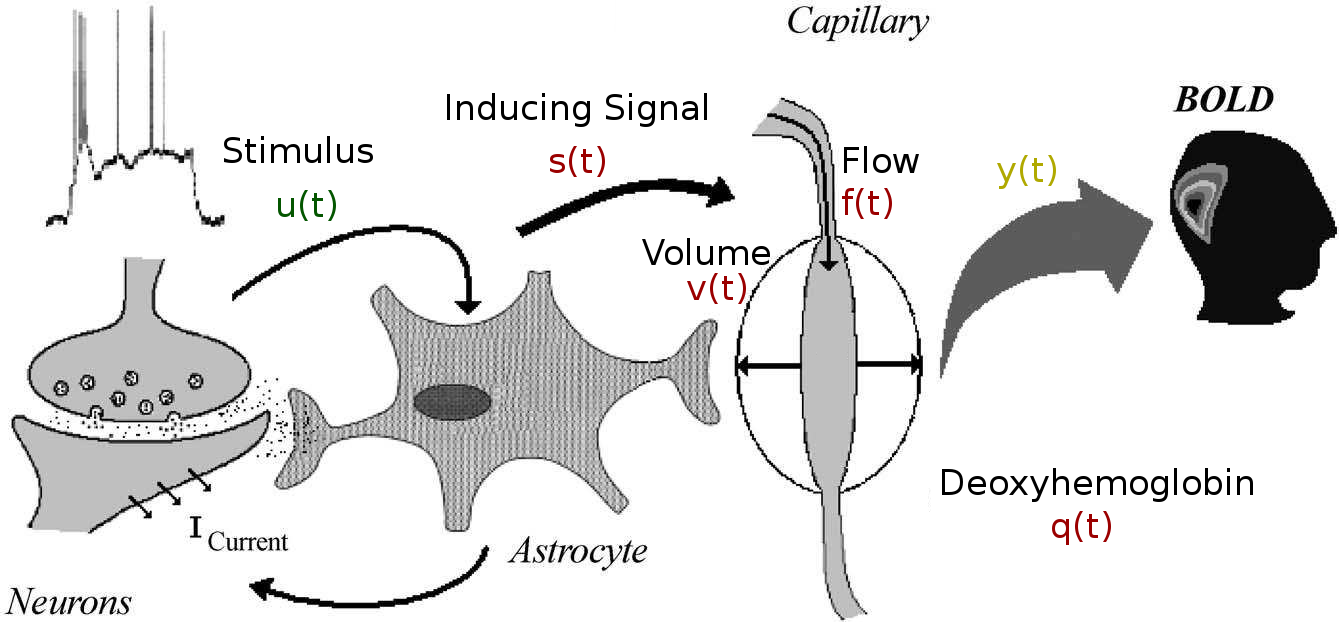
\includegraphics[width=10cm]{model2}
\caption{
    \tiny
    \cite{Riera2003}
}
\end{figure}
\note{Its been known for about 20 years that changes in Blood Oxygen Level alter
        T2$^*$ relaxation times. The basis of contrast in fMRI is 
        changes in the so-called spin-spin relaxation (or T2$^*$ relaxation time
        of tissue). The rate of loss in nuclear spin coherence depends on the molecules in the voxel being
        measured \emph{and the surrounding voxels}. For this reason the signal 
        detected from BLOOD doesn't just depend on the amount of oxygen, but also the
        amount of De-oxygenated hemoglobin. The question then, is what drives changes
        in De-oxygenated Hemoglobin and blood volume?
        
        Well the brain has no local oxygen storage, so it is completely dependent on 
        fresh Oxygenated-Hemoglobin. When the brain becomes more active, firing rates
        for neurons increase by several orders of magnitude, and recharging these neurons
        requires additional oxygen for matabolism. }
\note{Rates from below 1 Hz to 5 to 6 Hundred Hz}
\note{Change in average firing rates increase metabolism and sympathetic response causes
        increased inflow of oxygenated blood.}
\note{In the version of the Balloon model I used, the flow is locked to metabolism.}
\note{According the balloon model this increases the local blood volume, and the outflow pressure.}
\note{So the signal is altered by changes in the ratio of Deoxyhemoglobin and Oxygenated Hemoglobin,
        which are a function of Volume and Oxygenation.}
\end{frame}

\begin{frame}{Activation Chain}
\begin{figure}
    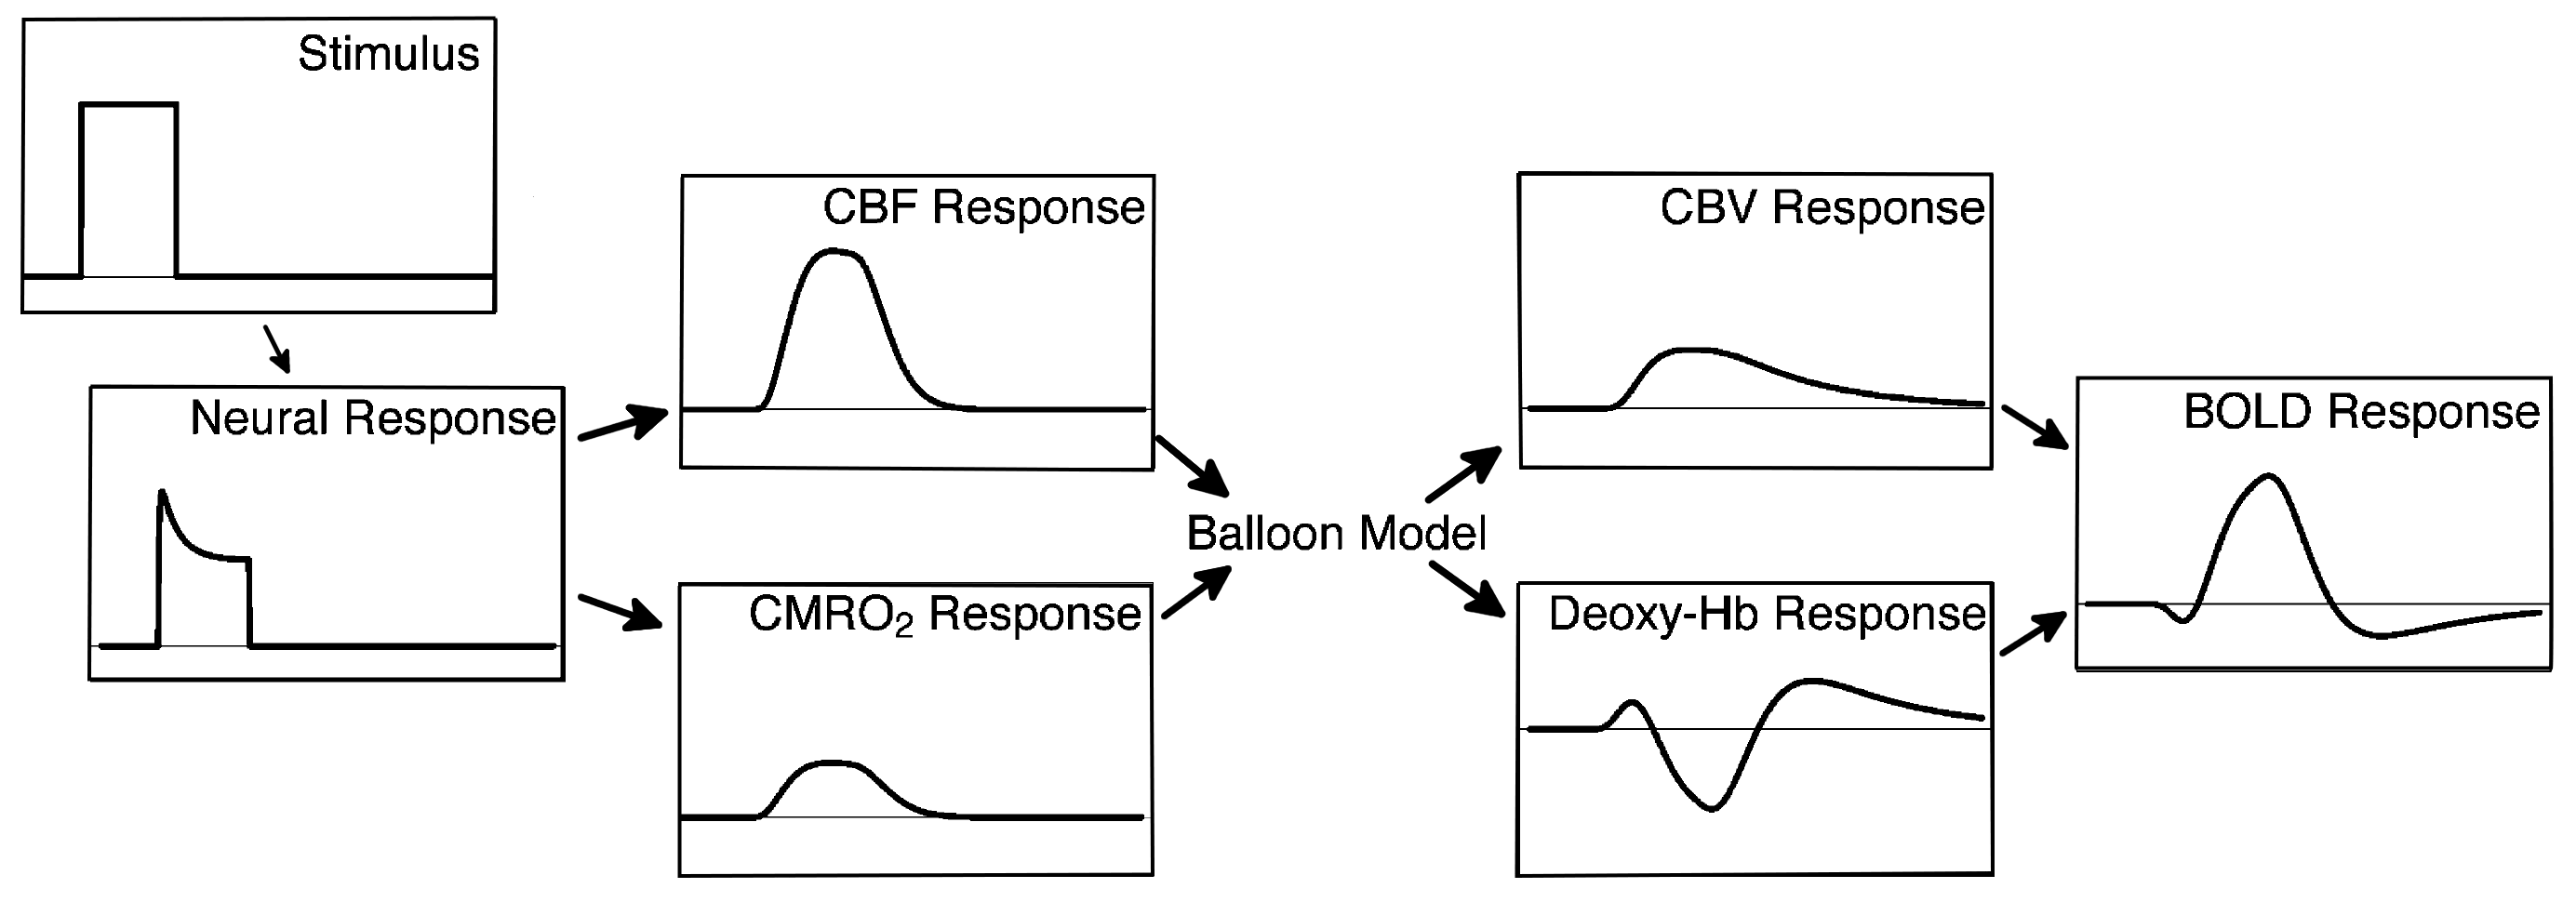
\includegraphics[width=\textwidth]{graphs}
\caption{
    \tiny
    \cite{Buxton2004}
}
\end{figure}
\end{frame}

%more expansion of all the parameters
\begin{frame}{BOLD State Space Model}
  \scriptsize
  \begin{columns}
  \begin{column}{.7\textwidth}
    \begin{itemize}
    \item State Vector:
    \begin{eqnarray}
    \color{mblue}\dot{s}(t) &=& {\color{mred}\epsilon} {\color{mgreen}u(t)} - 
                \frac{\color{mblue}s(t)}{\color{mred}\tau_s} - \frac{{\color{mblue}f(t)}-1}{\color{mred}\tau_f} \nonumber \\
    \color{mblue}\dot{f}(t) &=& \color{mblue}s \nonumber \\
    \color{mblue}\dot{v}(t) &=& \frac{{\color{mblue}f(t)} - 
                {\color{mblue}v(t)} ^ {1/{\color{mred}\alpha}}}{\color{mred}\tau_0} \nonumber \\
    \color{mblue}\dot{q}(t) &=& \frac{1}{\color{mred}\tau_0}
            \left(\frac{{\color{mblue}f(t)}(1-(1-{\color{mred}E_0})^{1/\color{mblue}f(t)})}{\color{mred}E_0} -
        \frac{\color{mblue}q(t)}{{\color{mblue}v(t)}^{1-1/\color{mred}\alpha}}\right) \nonumber 
    \end{eqnarray}
    \item Output:
    $${\color{myellow}y(t)} = {\color{mred}V_0}(a_1( 1 - {\color{mblue}Q(t)}) - a_2(1 - {\color{mblue}V(t)}))$$
    \end{itemize}
  \end{column}

  \begin{column}{.3\textwidth}
    \begin{itemize}
        \item State Variables:
        $${\color{mblue}s(t)}, {\color{mblue}f(t)}, {\color{mblue}v(t)}, {\color{mblue}q(t)}$$
        \item Parameters:
        $${\color{mred}\epsilon}, {\color{mred}\tau_s}, {\color{mred}\tau_f}, {\color{mred}\alpha}, 
                    {\color{mred}\tau_0}, {\color{mred}E_0}, {\color{mred}V_0}$$
        \item Constants:
        $$a_1, a_2$$
        \item Input:
        $$\color{mgreen}u(t)$$
    \end{itemize}
  \end{column}
  \end{columns}
  \note{System is dissipative:\\
  If no input is provided, it will rather quickly decay.\\
  Constant input leads to steady state response.\\
  First term in $\dot{q}$ is the metabolism term.\\
  Outflow is the $v^{1/\alpha}$ term\\
  Significant nonlinearity.}
\end{frame}

\section{Nonlinear Regression}
\subsection{Prior Works}
\begin{frame}{Approximation Method}
  \begin{itemize}
    \item Canonical Hemodynamic Response Function
    \begin{itemize}
        \item No Parameters Estimated
        \item Maximum Likelihood Possible
        \item Inflexible - even to changes in onset time
    \end{itemize}
    \item 2nd Order Volterra Kernel \cite{Friston2000}
    \begin{itemize}
        \item Quadratic Convolution used to approximate Jacobian Matrix.
        \item Volterra approximation quality is not known.
    \end{itemize}
    {\footnotesize
    $$y(t) = k_0 + \int_{-\infty}^{\infty} k_1(s_1) x(t-s_1) ds_1
        + \int_{-\infty}^{\infty} k_2(s_1,s_2) x(t-s_1)x(t-s_2) ds_1 ds_2$$
    }
    \begin{center}
    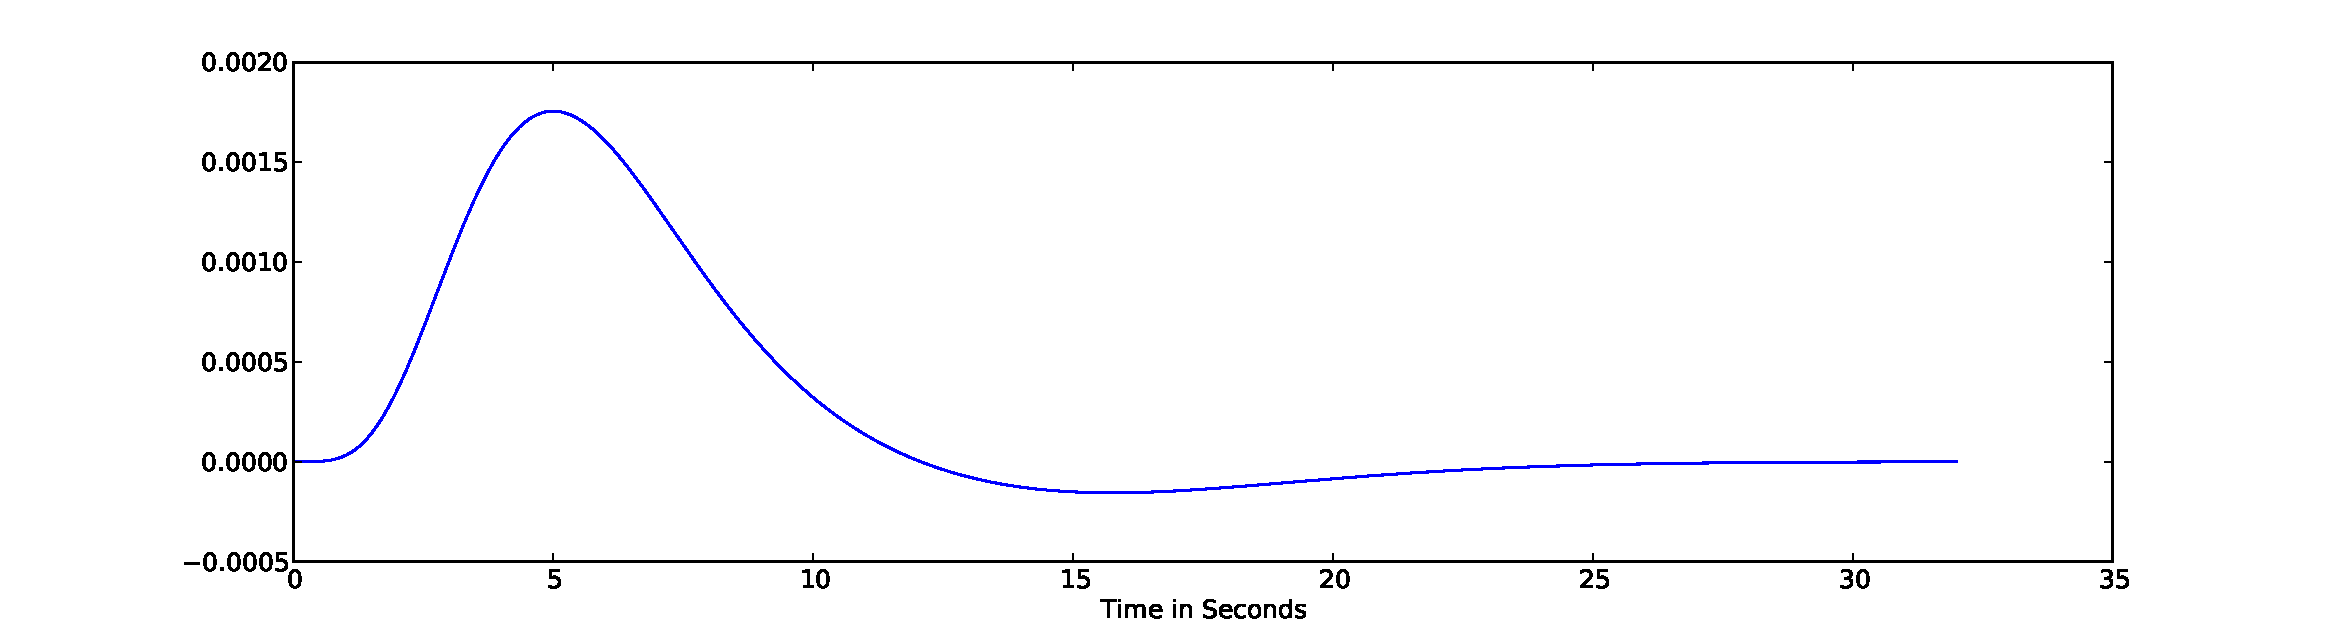
\includegraphics[clip=true,trim=4.88cm 0cm 5cm 1.5cm,height=2.7cm,width=8cm]{HRF}
    \end{center}
    
  \end{itemize}
  \note{
    \begin{itemize}
        \item Neither of these is truly nonlinear method
        \item General Linear Model uses a generic Kernel across all
                regions.
        \item Canonical Hemodynamic Response Function
        \item Fast, Maximum Likelihood, Not Adaptive, same across regions/patients
                pathologies
        \item Volterra Kernel Potentially Offers a Better Fit
        \item If Kernels Could be quickly optimized, it could work
        \item Never really used, because optimizing kernels is slow, and
                its still an approximation
    \end{itemize}
  }
\end{frame}

\begin{frame}{Nonlinear Methods}
\begin{itemize}
    \begin{columns}
    \begin{column}{.45\textwidth}
    \item Local Linearization filter, \cite{Riera2003}
    $$f(t)- f(t-1) \sim N(0, \sigma^2)$$
    \item Genetic Algorithms and Simulated Annealing, \cite{Vakorin2007}
    \item Unscented Kalman Filter \cite{Hu2009}
    \item Particle Filters to estimate States, \cite{Murray2009}
    \begin{itemize}
        \item ML estimate of $\Theta$, \cite{Johnston2007}
    \end{itemize}
    \end{column}

    \begin{column}{.55\textwidth}
    \begin{figure}
    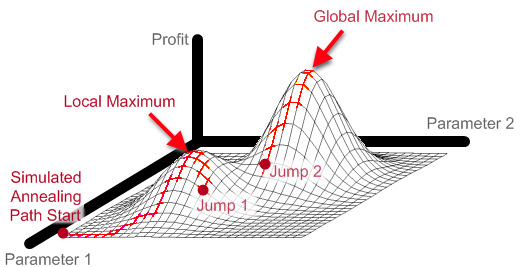
\includegraphics[clip=true,trim=0cm 0cm 0cm 1cm,width=.6\textwidth]{simulated_annealing}
    \caption{Simulated Annealing can escape local minima with chaotic jumps. \cite{Dama}}
    \end{figure}
    \begin{figure}
    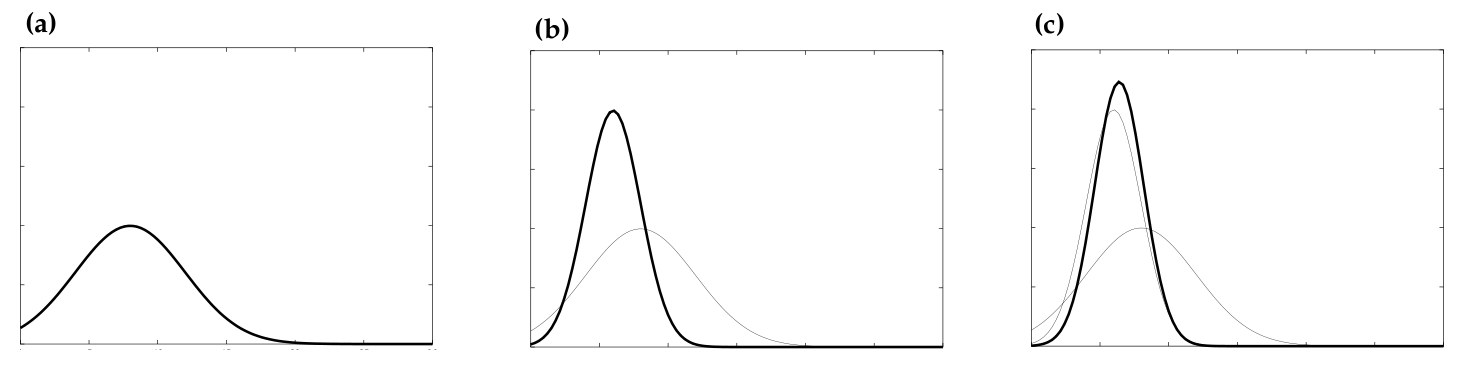
\includegraphics[width=\textwidth]{kalman}
    \caption{UKF: (a) Initial Belief  (b) Noisy Measurement  (c) incorporated into the belief. \cite{Thrun2005}}
    \end{figure}
    \end{column}
    \end{columns}
\end{itemize}
\note{
    \tiny
    \begin{itemize}
     \item Riera: Local Linearize
        \begin{itemize}
            \tiny
            \item Compare Estimated Step (Adjacent Measurements) With Actual Step
            \item Jacobian is available - gradient descent possible
            \item Removes Drift/Structured Noise
            \item Completely Removes DC component - 
            \item Quality Depends on experimental design: less Effective For 
                    Block Stimulus
        \end{itemize}
        \item Vakorin: GA used to optimize spike train, Simulated Annealing 
            to Estimate Parameters
        \item Simulated Annealing is Slow, every step: BOLD recalc
        \item UKF linearizes the noise, propagates limited number of 
                samples through the state equation, and then uses 
                first 2 moments
        \item Murray kept parameters constant, all differences result of 
            state-noise
        \item Johnston - used estimated state distribution to perform
                maximum likelihood on other parameters.
        \item ($P(X, \Theta | Y) = P(X | Y, \Theta) P(\Theta | Y)$)
        \item Johnston's Results don't mesh
        \item Neither of previous particle filter methods considered it
                possible 
        \item All of these methods focus on point estimate of the solution
    \end{itemize}
}
\end{frame}

\subsection{Particle Filter}
%frame with example
\begin{frame}{Example System Identification}
\begin{itemize}
\item Given:
    \begin{itemize}
    \item Elevation Map (1D)
    \item Ability To Measure Elevation
    \end{itemize}
\item Particle Consists of the unknowns:
    \begin{itemize}
    \item State: Location  $[0, 20]$
    \item Constant: Direction  $\{Left, Right\}$
    \end{itemize}
\end{itemize}

\begin{center}
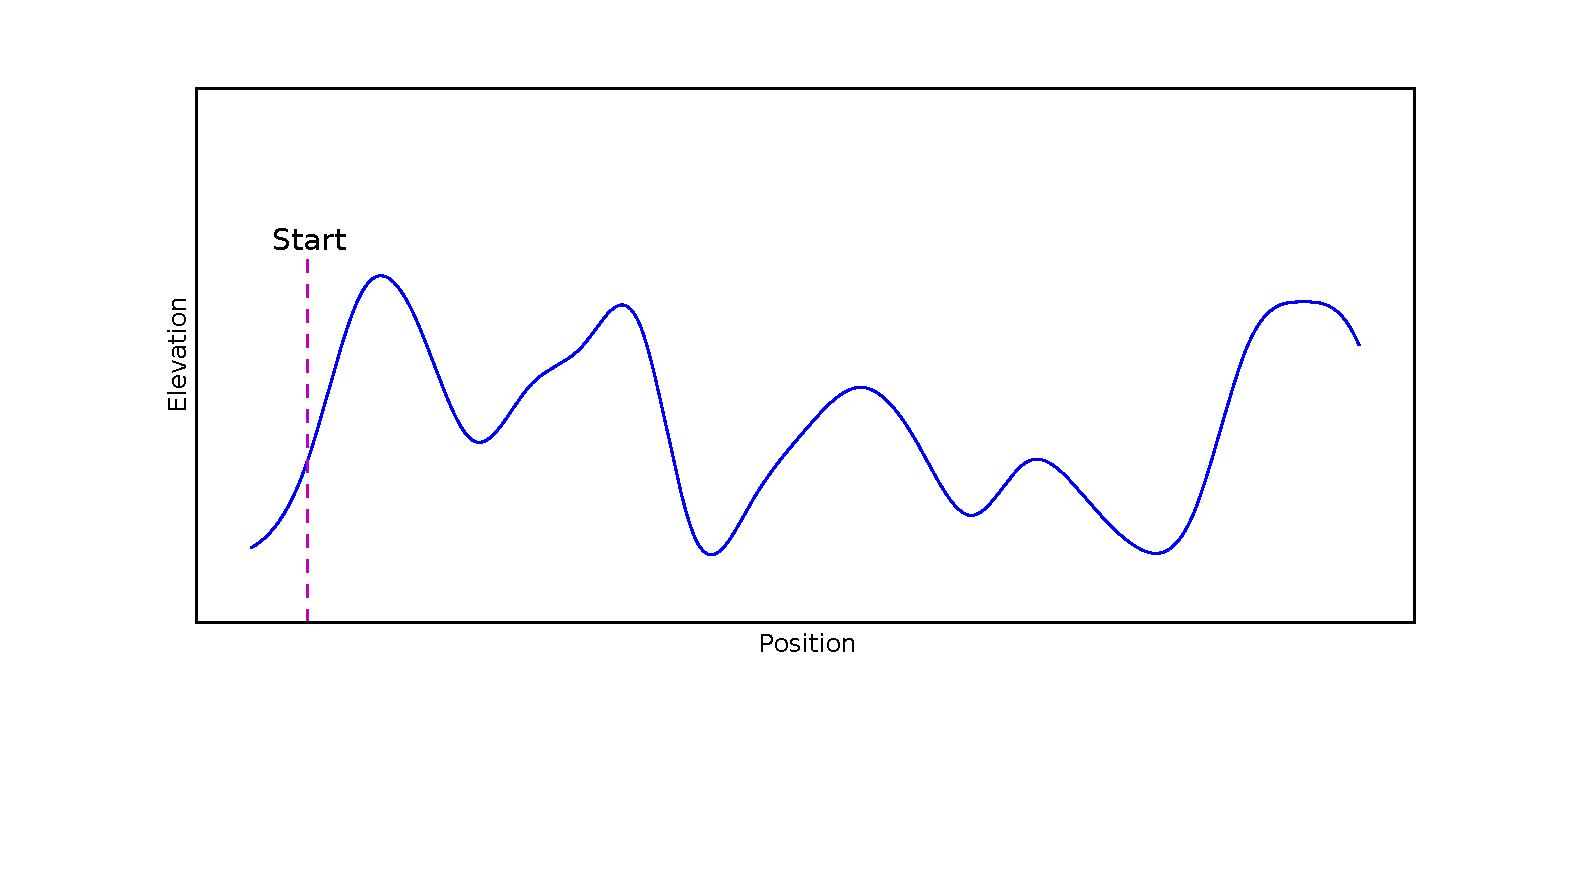
\includegraphics[clip=true,trim=2cm 3cm 3cm 3cm,width=.7\textwidth]{setup}
\end{center}
\note{
\begin{itemize}
    \item Start with an example.
    \item One dimensional mountain range
    \item Have a map and an altimeter to measure elevation
    \item Don't know where you are or which direction you are moving
    \item Need a prior distribution that spans both dims direction/location
\end{itemize}
}
\end{frame}

\begin{frame}{Initial Distribution}
\centering
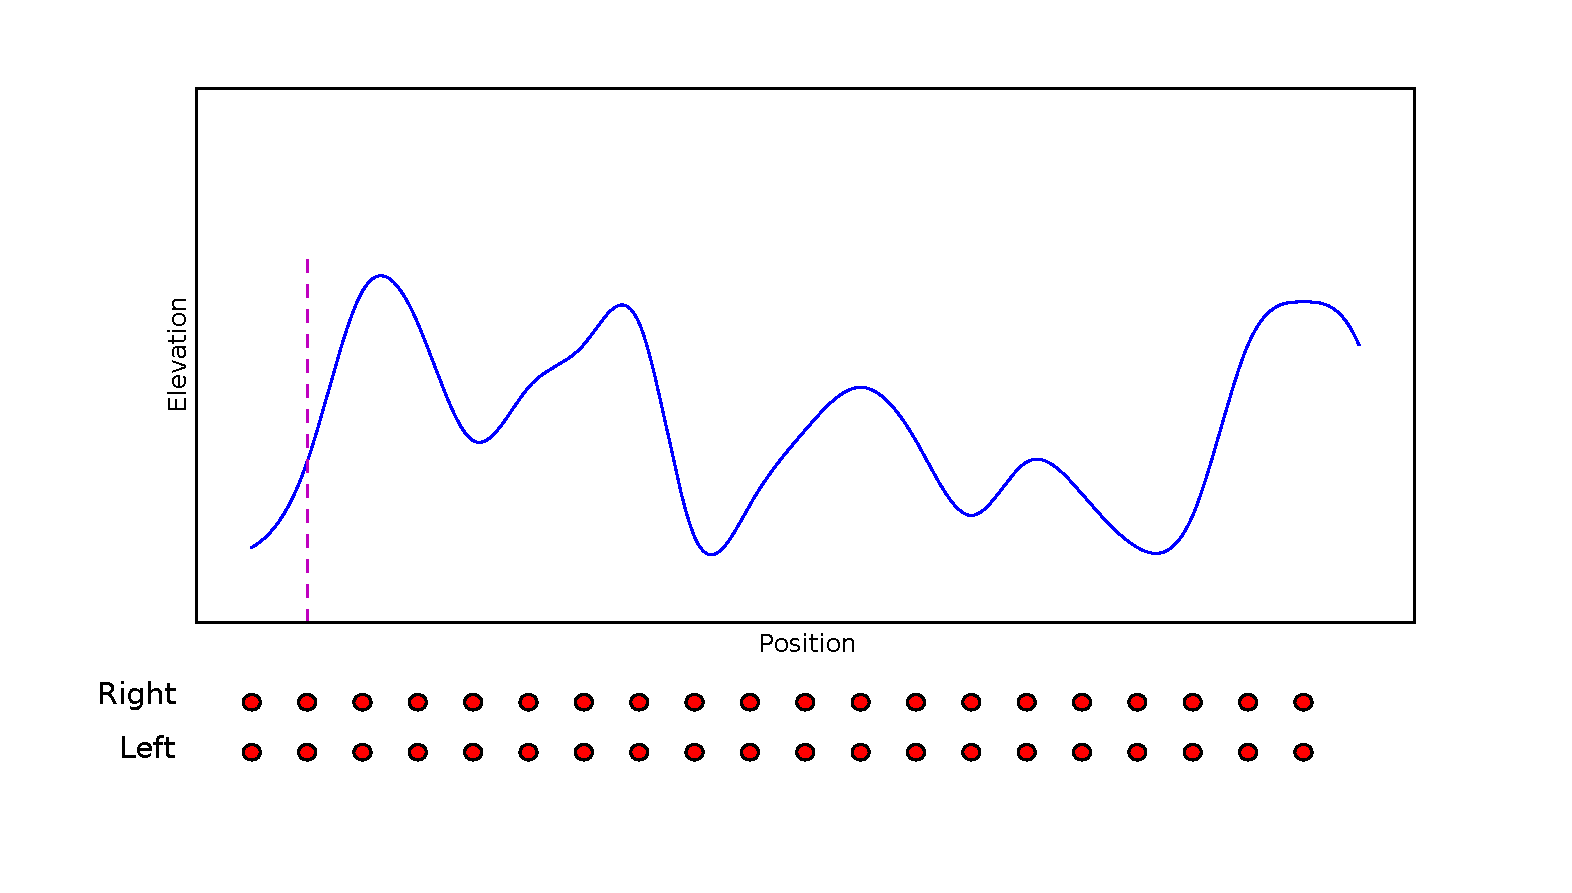
\includegraphics[width=\textwidth]{init}
\note{
\begin{itemize}
    \item Here is the prior, 20 locations, either right or left, 
        40 total particles
    \item So each particle contains a unique direction and position
\end{itemize}
}

\end{frame}

\begin{frame}{Measurement 1}
\centering
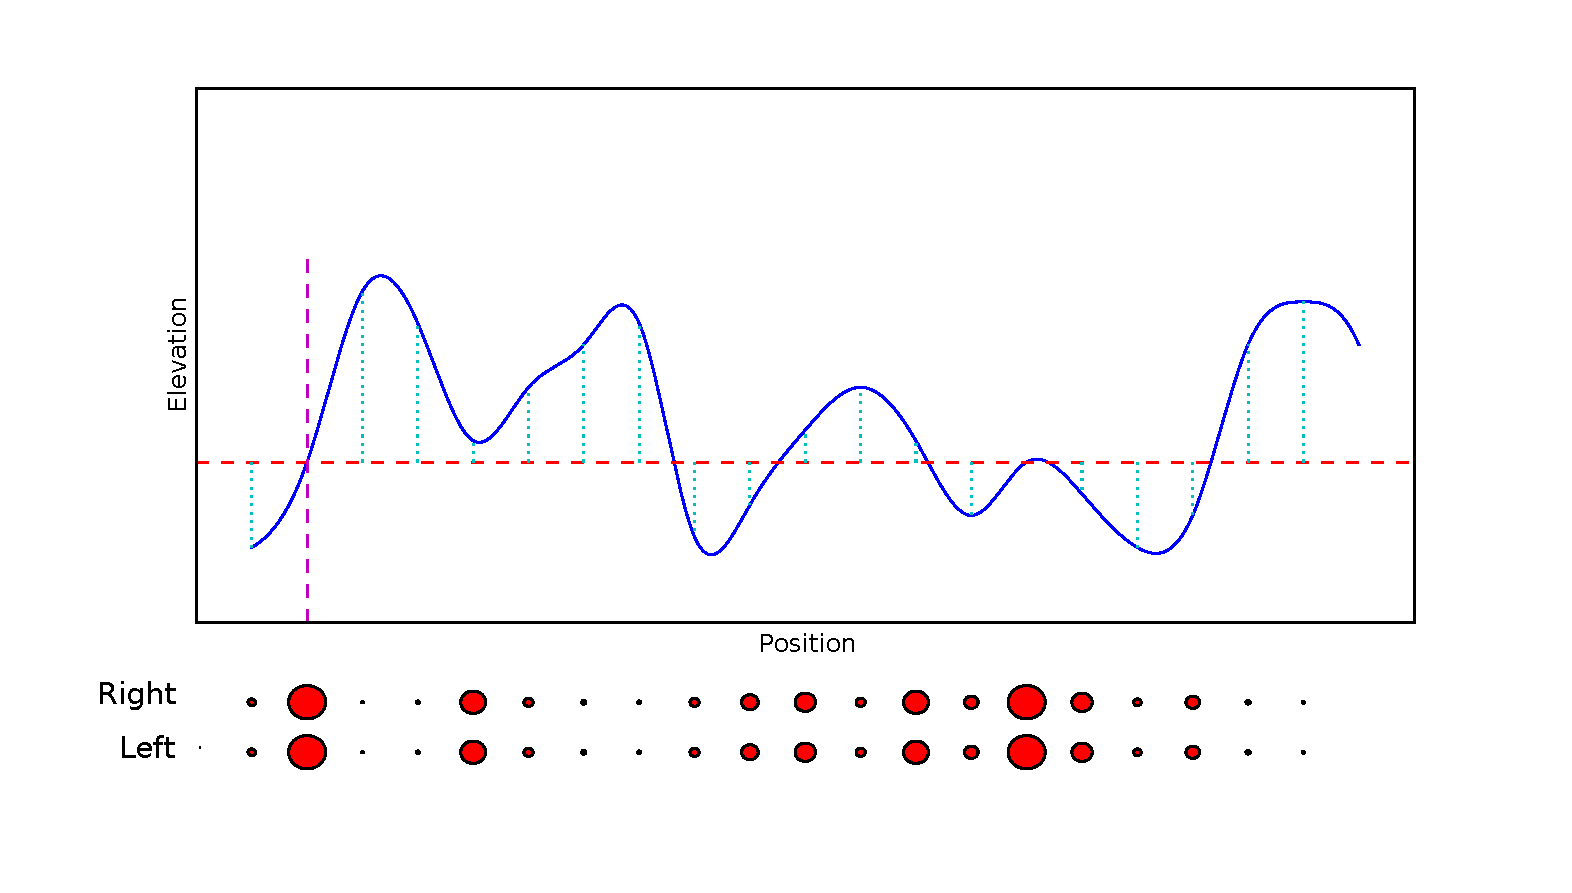
\includegraphics[width=\textwidth]{meas1}
\note{
\begin{itemize}
    \item Now measure the elevation, and weight locations that are close
            to that elevation higher
    \item Note the second downhill, No particles nearby in terms of $\Delta y$.
    \item Compare that to the next uphill
    \item Relation between particle spacing and weighting function
    \item Now we've applied a measurement, now need to integrate state
            until the next measurement becomes available.
\end{itemize}
}
\end{frame}

\begin{frame}{Step Forward}
\centering
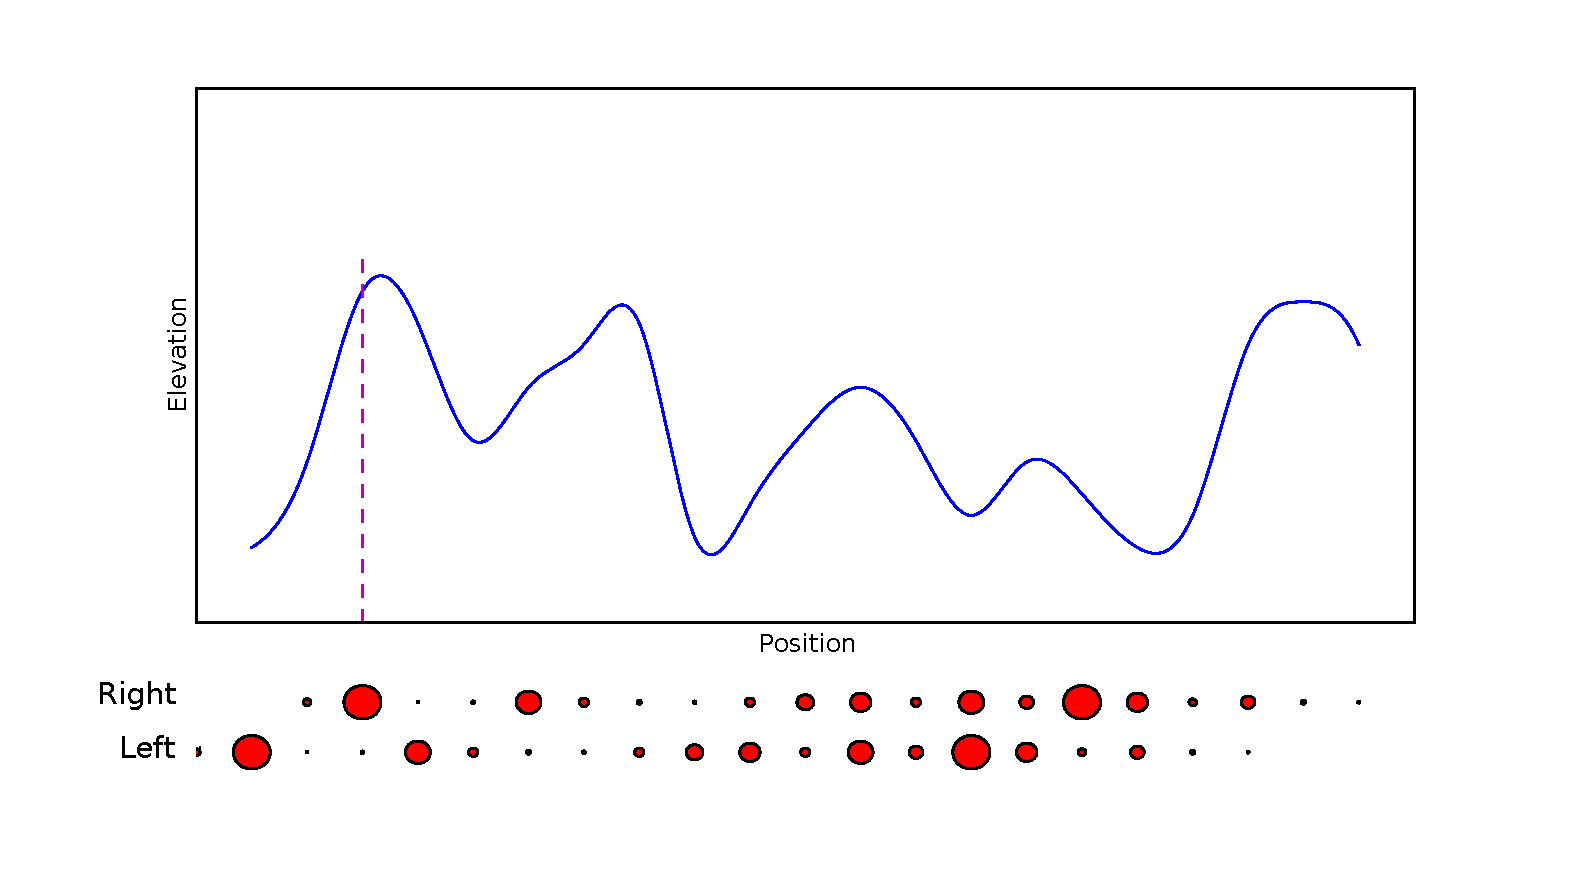
\includegraphics[width=\textwidth]{move1}
\note{
    \begin{itemize}
    \item Notice that no movement occurs in terms of right/left. Those
            are parameters and so they don't change with time.
    \end{itemize}
}
\end{frame}

\begin{frame}{Measurement 2}
\centering
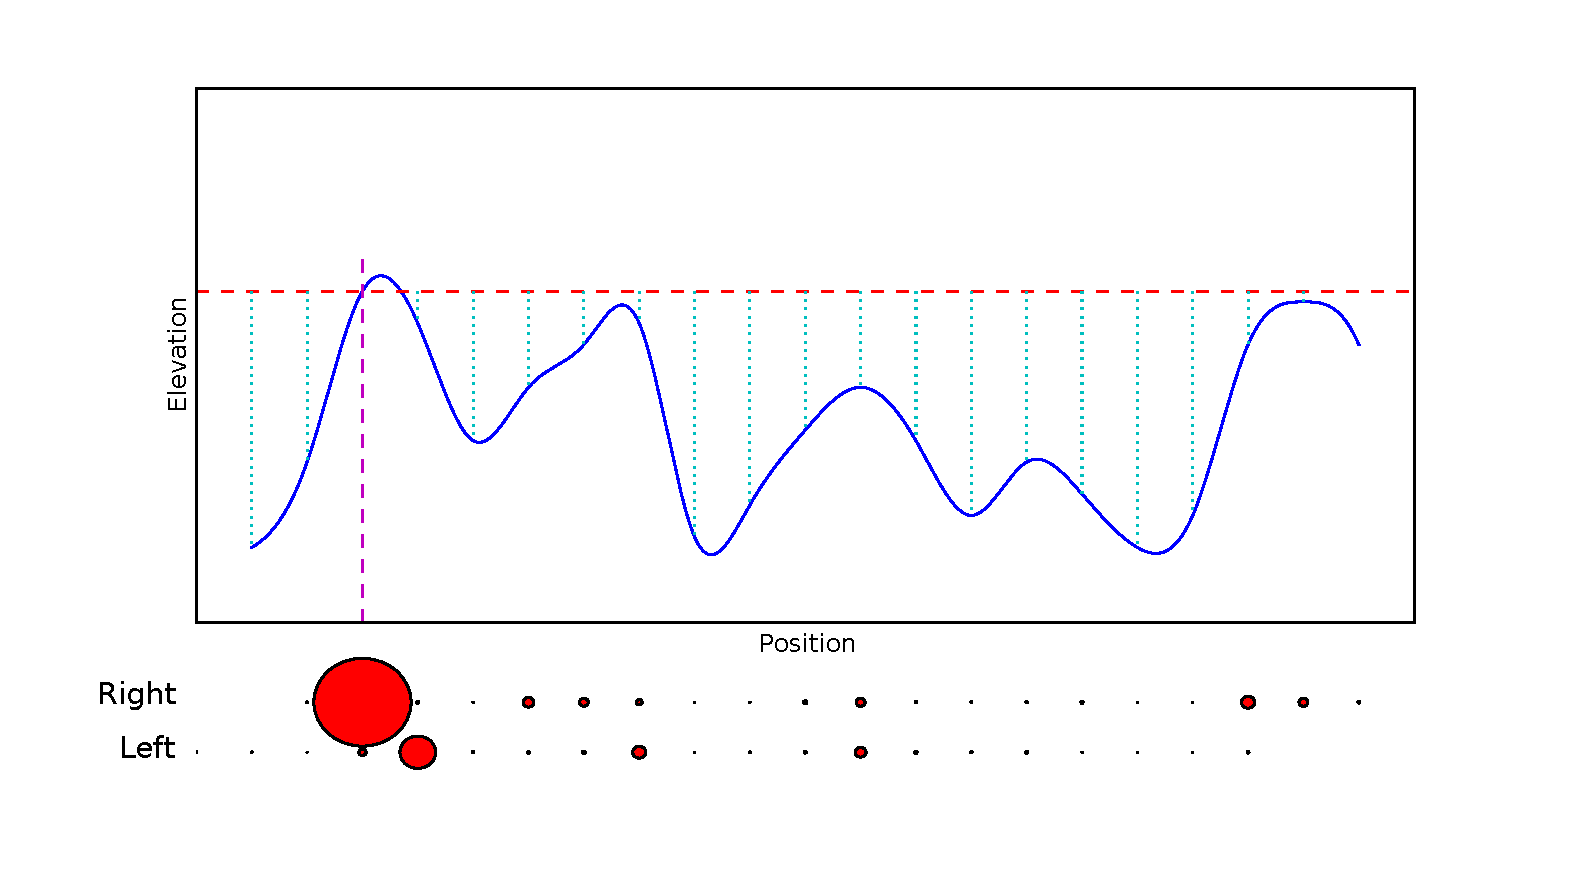
\includegraphics[width=\textwidth]{meas2}\\
\note{
\begin{itemize}
    \item So the true location now how been correct twice in a row.
    \item Note that traveling left over the hill results in similar 
            measurements
\end{itemize}
}
\end{frame}

\begin{frame}{Step Forward}
\centering
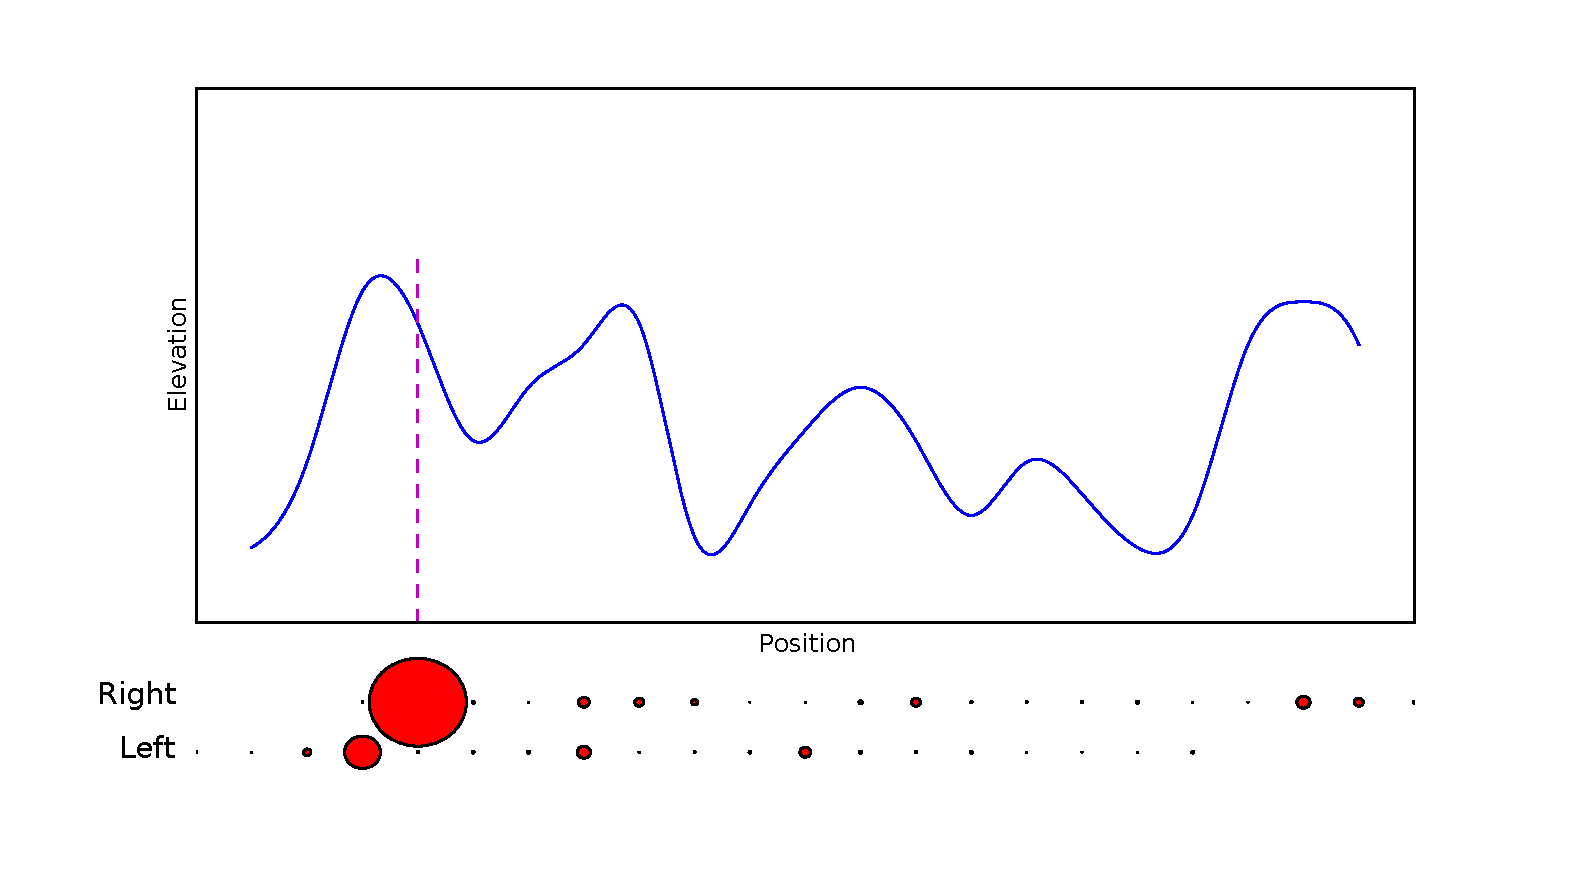
\includegraphics[width=\textwidth]{move2}\\
\end{frame}

\begin{frame}{Particle Filter Concepts}
\small
\begin{columns}
\begin{column}{.5\textwidth}
\begin{itemize}
    \item Weighting Function
        \begin{itemize}
            \item Converts Discrete Estimates of $y$ 
                    Into a Continuous Estimate of $y$
        \end{itemize}
    \item Particle Density
    \item Resampling
    \begin{itemize}
        \item Remove Useless Particles
    \end{itemize}
    \item Regularized Resampling
    \begin{itemize}
        \item Prevent Identical Particles
    \end{itemize}
\end{itemize}
\end{column}

\begin{column}{.5\textwidth}
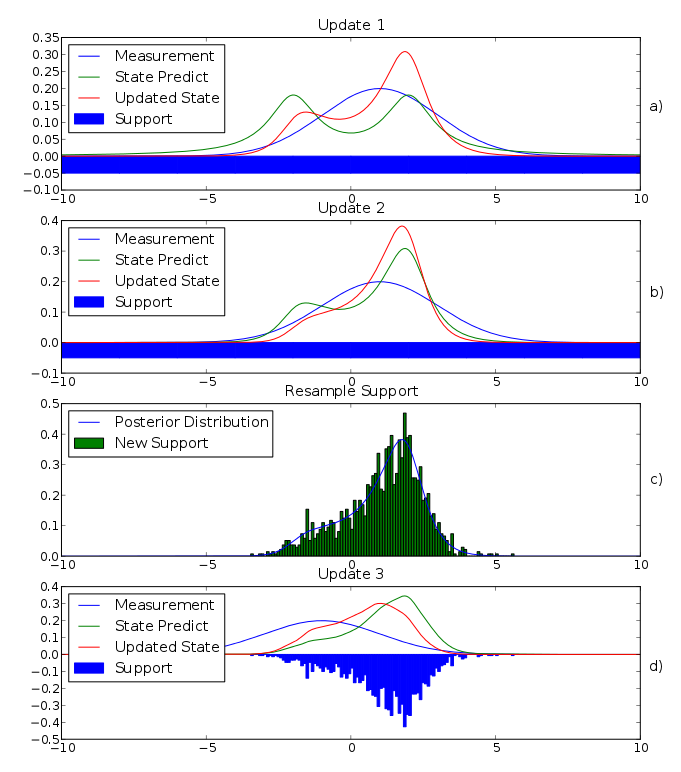
\includegraphics[clip=true,trim=.75cm 7.07cm .5cm 7cm,width=\textwidth]{particle_filter2}
\end{column}
\end{columns}
\note{
    \tiny
\begin{itemize}
    \item Weighting function decides how much you want to weight particles
            that don't exactly match the measurement
    \item The weighting function and the particle density 
            (distance between particles) form a sort of net
    \item Whether the net has holes also depends on the maximum gradient
            of $y$ with respect to the parameters
    \item Resampling allows the algorithm to increase density in areas
            of interest. 
    \item Resampling could also remove "good" areas
    \item Resampling typically draws from the set of existing particles,
            reducing the number of unique particles
    \item Regularized resampling, instead draws from a smooth version of
            the posterior distribution, so particles are always unique
\end{itemize}
}
\end{frame}

\begin{frame}{Particle Construction, Particle $i$, Time $k$}
\begin{columns}
\begin{column}{.54\textwidth}
\begin{itemize}
    \item Mixture PDF, with $N_p$ particles:
        $$P(x_k) = \sum_{i=0}^{N_p} w_k^i\delta(x_k - x^i_k )$$
    \item Weight Definition:
        $$w^i_k \propto \frac{P(x^i_{0:k} | y_{0:k})}{q(x^i_{0:k} | y_{0:k})}$$
    \item Incorporating Measurement $y_k$:
        $$w^i_k \propto & w^i_{k-1}P(y_k| x^i_k) $$
\end{itemize}
\end{column}

\begin{column}{.46\textwidth}
\tiny
\ifx\du\undefined
  \newlength{\du}
\fi
\setlength{\du}{10\unitlength}
\begin{tikzpicture}
\pgftransformxscale{1.000000}
\pgftransformyscale{-1.000000}
\definecolor{dialinecolor}{rgb}{0.000000, 0.000000, 0.000000}
\pgfsetstrokecolor{dialinecolor}
\definecolor{dialinecolor}{rgb}{1.000000, 1.000000, 1.000000}
\pgfsetfillcolor{dialinecolor}
\pgfsetlinewidth{0.050000\du}
\pgfsetdash{}{0pt}
\definecolor{dialinecolor}{rgb}{1.000000, 1.000000, 1.000000}
\pgfsetfillcolor{dialinecolor}
\fill (9.250000\du,3.650000\du)--(9.250000\du,5.050000\du)--(12.1000\du,5.050000\du)--(12.1000\du,3.650000\du)--cycle;
\definecolor{dialinecolor}{rgb}{0.000000, 0.000000, 0.000000}
\pgfsetstrokecolor{dialinecolor}
\draw (9.250000\du,3.650000\du)--(9.250000\du,5.050000\du)--(12.1000\du,5.050000\du)--(12.1000\du,3.650000\du)--cycle;
% setfont left to latex
\definecolor{dialinecolor}{rgb}{0.000000, 0.000000, 0.000000}
\pgfsetstrokecolor{dialinecolor}
\node at (10.732500\du,4.600000\du){Particle};
\definecolor{dialinecolor}{rgb}{1.000000, 1.000000, 1.000000}
\pgfsetfillcolor{dialinecolor}
\fill (9.250000\du,5.050000\du)--(9.250000\du,14.050000\du)--(12.1000\du,14.050000\du)--(12.1000\du,5.050000\du)--cycle;
\definecolor{dialinecolor}{rgb}{0.000000, 0.000000, 0.000000}
\pgfsetstrokecolor{dialinecolor}
\draw (9.250000\du,5.050000\du)--(9.250000\du,14.050000\du)--(12.1000\du,14.050000\du)--(12.1000\du,5.050000\du)--cycle;
% setfont left to latex
\definecolor{dialinecolor}{rgb}{0.000000, 0.000000, 0.000000}
\pgfsetstrokecolor{dialinecolor}
\node[anchor=west] at (9.400000\du,5.750000\du){\color{mblue} $s$};
% setfont left to latex
\definecolor{dialinecolor}{rgb}{0.000000, 0.000000, 0.000000}
\pgfsetstrokecolor{dialinecolor}
\node[anchor=west] at (9.400000\du,6.550000\du){\color{mblue} $f$};
% setfont left to latex
\definecolor{dialinecolor}{rgb}{0.000000, 0.000000, 0.000000}
\pgfsetstrokecolor{dialinecolor}
\node[anchor=west] at (9.400000\du,7.350000\du){\color{mblue} $q$};
% setfont left to latex
\definecolor{dialinecolor}{rgb}{0.000000, 0.000000, 0.000000}
\pgfsetstrokecolor{dialinecolor}
\node[anchor=west] at (9.400000\du,8.150000\du){\color{mblue} $v$};
% setfont left to latex
\definecolor{dialinecolor}{rgb}{0.000000, 0.000000, 0.000000}
\pgfsetstrokecolor{dialinecolor}
\node[anchor=west] at (9.400000\du,8.950000\du){\color{mred} $\epsilon$};
% setfont left to latex
\definecolor{dialinecolor}{rgb}{0.000000, 0.000000, 0.000000}
\pgfsetstrokecolor{dialinecolor}
\node[anchor=west] at (9.400000\du,9.750000\du){\color{mred} $\tau_f$};
% setfont left to latex
\definecolor{dialinecolor}{rgb}{0.000000, 0.000000, 0.000000}
\pgfsetstrokecolor{dialinecolor}
\node[anchor=west] at (9.400000\du,10.550000\du){\color{mred} $\tau_s$};
% setfont left to latex
\definecolor{dialinecolor}{rgb}{0.000000, 0.000000, 0.000000}
\pgfsetstrokecolor{dialinecolor}
\node[anchor=west] at (9.400000\du,11.350000\du){\color{mred} $\tau_0$};
% setfont left to latex
\definecolor{dialinecolor}{rgb}{0.000000, 0.000000, 0.000000}
\pgfsetstrokecolor{dialinecolor}
\node[anchor=west] at (9.400000\du,12.150000\du){\color{mred} $\alpha$};
% setfont left to latex
\definecolor{dialinecolor}{rgb}{0.000000, 0.000000, 0.000000}
\pgfsetstrokecolor{dialinecolor}
\node[anchor=west] at (9.400000\du,12.950000\du){\color{mred} $E_0$};
% setfont left to latex
\definecolor{dialinecolor}{rgb}{0.000000, 0.000000, 0.000000}
\pgfsetstrokecolor{dialinecolor}
\node[anchor=west] at (9.400000\du,13.750000\du){\color{mred} $V_0$};
\definecolor{dialinecolor}{rgb}{1.000000, 1.000000, 1.000000}
\pgfsetfillcolor{dialinecolor}
\fill (9.250000\du,14.050000\du)--(9.250000\du,15.050000\du)--(12.1000\du,15.050000\du)--(12.1000\du,14.050000\du)--cycle;
\definecolor{dialinecolor}{rgb}{0.000000, 0.000000, 0.000000}
\pgfsetstrokecolor{dialinecolor}
\draw (9.250000\du,14.050000\du)--(9.250000\du,15.050000\du)--(12.1000\du,15.050000\du)--(12.1000\du,14.050000\du)--cycle;
% setfont left to latex
\definecolor{dialinecolor}{rgb}{0.000000, 0.000000, 0.000000}
\pgfsetstrokecolor{dialinecolor}
\node[anchor=west] at (9.400000\du,14.750000\du){ weight};
% setfont left to latex
\definecolor{dialinecolor}{rgb}{0.000000, 0.000000, 0.000000}
\pgfsetstrokecolor{dialinecolor}
\node[anchor=west] at (5.050000\du,5.850000\du){};
% setfont left to latex
\definecolor{dialinecolor}{rgb}{0.000000, 0.000000, 0.000000}
\pgfsetstrokecolor{dialinecolor}
\node[anchor=west] at (5.100000\du,6.500000\du){Change};
% setfont left to latex
\definecolor{dialinecolor}{rgb}{0.000000, 0.000000, 0.000000}
\pgfsetstrokecolor{dialinecolor}
\node[anchor=west] at (5.100000\du,7.300000\du){With Time};
% setfont left to latex
\definecolor{dialinecolor}{rgb}{0.000000, 0.000000, 0.000000}
\pgfsetstrokecolor{dialinecolor}
\node[anchor=west] at (13.000000\du,9.850000\du){Change When};
% setfont left to latex
\definecolor{dialinecolor}{rgb}{0.000000, 0.000000, 0.000000}
\pgfsetstrokecolor{dialinecolor}
\node[anchor=west] at (13.000000\du,10.650000\du){Resampling};
\pgfsetlinewidth{0.050000\du}
\pgfsetdash{}{0pt}
\pgfsetdash{}{0pt}
\pgfsetbuttcap
{
\definecolor{dialinecolor}{rgb}{0.000000, 0.000000, 0.000000}
\pgfsetfillcolor{dialinecolor}
% was here!!!
\definecolor{dialinecolor}{rgb}{0.000000, 0.000000, 0.000000}
\pgfsetstrokecolor{dialinecolor}
\pgfpathmoveto{\pgfpoint{9.000025\du}{5.399967\du}}
\pgfpatharc{217}{144}{1.000000\du and 1.000000\du}
\pgfusepath{stroke}
}
\pgfsetlinewidth{0.050000\du}
\pgfsetdash{}{0pt}
\pgfsetdash{}{0pt}
\pgfsetbuttcap
{
\definecolor{dialinecolor}{rgb}{0.000000, 0.000000, 0.000000}
\pgfsetfillcolor{dialinecolor}
% was here!!!
\definecolor{dialinecolor}{rgb}{0.000000, 0.000000, 0.000000}
\pgfsetstrokecolor{dialinecolor}
\pgfpathmoveto{\pgfpoint{9.000025\du}{6.999967\du}}
\pgfpatharc{217}{144}{1.000000\du and 1.000000\du}
\pgfusepath{stroke}
}
\pgfsetlinewidth{0.050000\du}
\pgfsetdash{}{0pt}
\pgfsetdash{}{0pt}
\pgfsetbuttcap
{
\definecolor{dialinecolor}{rgb}{0.000000, 0.000000, 0.000000}
\pgfsetfillcolor{dialinecolor}
% was here!!!
\definecolor{dialinecolor}{rgb}{0.000000, 0.000000, 0.000000}
\pgfsetstrokecolor{dialinecolor}
\draw (9.000000\du,6.600000\du)--(8.600000\du,6.800000\du);
}
\pgfsetlinewidth{0.050000\du}
\pgfsetdash{}{0pt}
\pgfsetdash{}{0pt}
\pgfsetbuttcap
{
\definecolor{dialinecolor}{rgb}{0.000000, 0.000000, 0.000000}
\pgfsetfillcolor{dialinecolor}
% was here!!!
\definecolor{dialinecolor}{rgb}{0.000000, 0.000000, 0.000000}
\pgfsetstrokecolor{dialinecolor}
\draw (8.600000\du,6.800000\du)--(9.000000\du,7.000000\du);
}
\pgfsetlinewidth{0.050000\du}
\pgfsetdash{}{0pt}
\pgfsetdash{}{0pt}
\pgfsetbuttcap
{
\definecolor{dialinecolor}{rgb}{0.000000, 0.000000, 0.000000}
\pgfsetfillcolor{dialinecolor}
% was here!!!
\definecolor{dialinecolor}{rgb}{0.000000, 0.000000, 0.000000}
\pgfsetstrokecolor{dialinecolor}
\pgfpathmoveto{\pgfpoint{12.399753\du}{9.80\du}}
\pgfpatharc{10}{-9}{12.965299\du and 12.965299\du}
\pgfusepath{stroke}
}
\pgfsetlinewidth{0.050000\du}
\pgfsetdash{}{0pt}
\pgfsetdash{}{0pt}
\pgfsetbuttcap
{
\definecolor{dialinecolor}{rgb}{0.000000, 0.000000, 0.000000}
\pgfsetfillcolor{dialinecolor}
% was here!!!
\definecolor{dialinecolor}{rgb}{0.000000, 0.000000, 0.000000}
\pgfsetstrokecolor{dialinecolor}
\pgfpathmoveto{\pgfpoint{12.419203\du}{15.0\du}}
\pgfpatharc{10}{-9}{12.847799\du and 12.847799\du}
\pgfusepath{stroke}
}
\pgfsetlinewidth{0.050000\du}
\pgfsetdash{}{0pt}
\pgfsetdash{}{0pt}
\pgfsetbuttcap
{
\definecolor{dialinecolor}{rgb}{0.000000, 0.000000, 0.000000}
\pgfsetfillcolor{dialinecolor}
% was here!!!
\definecolor{dialinecolor}{rgb}{0.000000, 0.000000, 0.000000}
\pgfsetstrokecolor{dialinecolor}
\draw (12.400000\du,9.800000\du)--(13.019438\du,10.220000\du);
}
\pgfsetlinewidth{0.050000\du}
\pgfsetdash{}{0pt}
\pgfsetdash{}{0pt}
\pgfsetbuttcap
{
\definecolor{dialinecolor}{rgb}{0.000000, 0.000000, 0.000000}
\pgfsetfillcolor{dialinecolor}
% was here!!!
\definecolor{dialinecolor}{rgb}{0.000000, 0.000000, 0.000000}
\pgfsetstrokecolor{dialinecolor}
\draw (13.019438\du,10.220000\du)--(12.440000\du,10.760000\du);
}
% setfont left to latex
\definecolor{dialinecolor}{rgb}{0.000000, 0.000000, 0.000000}
\pgfsetstrokecolor{dialinecolor}
\node[anchor=west] at (4.000000\du,15.000000\du){Change When};
% setfont left to latex
\definecolor{dialinecolor}{rgb}{0.000000, 0.000000, 0.000000}
\pgfsetstrokecolor{dialinecolor}
\node[anchor=west] at (4.000000\du,15.800000\du){Incorporating Measurement};
\pgfsetlinewidth{0.050000\du}
\pgfsetdash{}{0pt}
\pgfsetdash{}{0pt}
\pgfsetbuttcap
{
\definecolor{dialinecolor}{rgb}{0.000000, 0.000000, 0.000000}
\pgfsetfillcolor{dialinecolor}
% was here!!!
\definecolor{dialinecolor}{rgb}{0.000000, 0.000000, 0.000000}
\pgfsetstrokecolor{dialinecolor}
\draw (9.000000\du,14.200000\du)--(8.600000\du,14.800000\du);
}
\pgfsetlinewidth{0.050000\du}
\pgfsetdash{}{0pt}
\pgfsetdash{}{0pt}
\pgfsetbuttcap
{
\definecolor{dialinecolor}{rgb}{0.000000, 0.000000, 0.000000}
\pgfsetfillcolor{dialinecolor}
% was here!!!
\definecolor{dialinecolor}{rgb}{0.000000, 0.000000, 0.000000}
\pgfsetstrokecolor{dialinecolor}
\draw (9.000000\du,15.000000\du)--(8.600000\du,14.800000\du);
}
\end{tikzpicture}

\end{column}
\end{columns}
\note{
    \tiny
    \begin{itemize}
        \item The posterior distribution is represented by a mixture
                PDF, where the probability of a discrete point is based
                on its relative weight.
        \item The definition of the weight function is given. 
        \item $q$ is the importance density, which is just the location
            of the particles. When you plug in the weights, that 
            term and the $\delta$ cancel and you are just left
            with the probability of getting that timeseries of 
            states given the timeseries of measurements.
        \item After some simplification, it comes out that weights
            can be updated with new measurements rather simply.
        \item On the right that each particle has an estimate
            for all of those states and unknown parameters.
        \item Weights Don't Integrate to 1.

    \end{itemize}
}
\end{frame}

%\ifx\du\undefined
%  \newlength{\du}
%\fi
%\setlength{\du}{10\unitlength}
%\begin{tikzpicture}
%\pgftransformxscale{1.000000}
%\pgftransformyscale{-1.000000}
%\definecolor{dialinecolor}{rgb}{0.000000, 0.000000, 0.000000}
%\pgfsetstrokecolor{dialinecolor}
%\definecolor{dialinecolor}{rgb}{1.000000, 1.000000, 1.000000}
%\pgfsetfillcolor{dialinecolor}
%\pgfsetlinewidth{0.050000\du}
%\pgfsetdash{}{0pt}
%\definecolor{dialinecolor}{rgb}{1.000000, 1.000000, 1.000000}
%\pgfsetfillcolor{dialinecolor}
%\fill (9.250000\du,3.650000\du)--(9.250000\du,5.050000\du)--(13.215000\du,5.050000\du)--(13.215000\du,3.650000\du)--cycle;
%\definecolor{dialinecolor}{rgb}{0.000000, 0.000000, 0.000000}
%\pgfsetstrokecolor{dialinecolor}
%\draw (9.250000\du,3.650000\du)--(9.250000\du,5.050000\du)--(13.215000\du,5.050000\du)--(13.215000\du,3.650000\du)--cycle;
%% setfont left to latex
%\definecolor{dialinecolor}{rgb}{0.000000, 0.000000, 0.000000}
%\pgfsetstrokecolor{dialinecolor}
%\node at (11.232500\du,4.600000\du){Particle};
%\definecolor{dialinecolor}{rgb}{1.000000, 1.000000, 1.000000}
%\pgfsetfillcolor{dialinecolor}
%\fill (9.250000\du,5.050000\du)--(9.250000\du,14.050000\du)--(13.215000\du,14.050000\du)--(13.215000\du,5.050000\du)--cycle;
%\definecolor{dialinecolor}{rgb}{0.000000, 0.000000, 0.000000}
%\pgfsetstrokecolor{dialinecolor}
%\draw (9.250000\du,5.050000\du)--(9.250000\du,14.050000\du)--(13.215000\du,14.050000\du)--(13.215000\du,5.050000\du)--cycle;
%% setfont left to latex
%\definecolor{dialinecolor}{rgb}{0.000000, 0.000000, 0.000000}
%\pgfsetstrokecolor{dialinecolor}
%\node[anchor=west] at (9.400000\du,5.750000\du){\color{mblue} $s$};
%% setfont left to latex
%\definecolor{dialinecolor}{rgb}{0.000000, 0.000000, 0.000000}
%\pgfsetstrokecolor{dialinecolor}
%\node[anchor=west] at (9.400000\du,6.550000\du){\color{mblue} $f$};
%% setfont left to latex
%\definecolor{dialinecolor}{rgb}{0.000000, 0.000000, 0.000000}
%\pgfsetstrokecolor{dialinecolor}
%\node[anchor=west] at (9.400000\du,7.350000\du){\color{mblue} $q$};
%% setfont left to latex
%\definecolor{dialinecolor}{rgb}{0.000000, 0.000000, 0.000000}
%\pgfsetstrokecolor{dialinecolor}
%\node[anchor=west] at (9.400000\du,8.150000\du){\color{mblue} $v$};
%% setfont left to latex
%\definecolor{dialinecolor}{rgb}{0.000000, 0.000000, 0.000000}
%\pgfsetstrokecolor{dialinecolor}
%\node[anchor=west] at (9.400000\du,8.950000\du){\color{mred} $\epsilon$};
%% setfont left to latex
%\definecolor{dialinecolor}{rgb}{0.000000, 0.000000, 0.000000}
%\pgfsetstrokecolor{dialinecolor}
%\node[anchor=west] at (9.400000\du,9.750000\du){\color{mred} $\tau_f$};
%% setfont left to latex
%\definecolor{dialinecolor}{rgb}{0.000000, 0.000000, 0.000000}
%\pgfsetstrokecolor{dialinecolor}
%\node[anchor=west] at (9.400000\du,10.550000\du){\color{mred} $\tau_s$};
%% setfont left to latex
%\definecolor{dialinecolor}{rgb}{0.000000, 0.000000, 0.000000}
%\pgfsetstrokecolor{dialinecolor}
%\node[anchor=west] at (9.400000\du,11.350000\du){\color{mred} $\tau_0$};
%% setfont left to latex
%\definecolor{dialinecolor}{rgb}{0.000000, 0.000000, 0.000000}
%\pgfsetstrokecolor{dialinecolor}
%\node[anchor=west] at (9.400000\du,12.150000\du){\color{mred} $\alpha$};
%% setfont left to latex
%\definecolor{dialinecolor}{rgb}{0.000000, 0.000000, 0.000000}
%\pgfsetstrokecolor{dialinecolor}
%\node[anchor=west] at (9.400000\du,12.950000\du){\color{mred} $\E_0$};
%% setfont left to latex
%\definecolor{dialinecolor}{rgb}{0.000000, 0.000000, 0.000000}
%\pgfsetstrokecolor{dialinecolor}
%\node[anchor=west] at (9.400000\du,13.750000\du){\color{mred} $V_0$};
%\definecolor{dialinecolor}{rgb}{1.000000, 1.000000, 1.000000}
%\pgfsetfillcolor{dialinecolor}
%\fill (9.250000\du,14.050000\du)--(9.250000\du,15.050000\du)--(13.215000\du,15.050000\du)--(13.215000\du,14.050000\du)--cycle;
%\definecolor{dialinecolor}{rgb}{0.000000, 0.000000, 0.000000}
%\pgfsetstrokecolor{dialinecolor}
%\draw (9.250000\du,14.050000\du)--(9.250000\du,15.050000\du)--(13.215000\du,15.050000\du)--(13.215000\du,14.050000\du)--cycle;
%% setfont left to latex
%\definecolor{dialinecolor}{rgb}{0.000000, 0.000000, 0.000000}
%\pgfsetstrokecolor{dialinecolor}
%\node[anchor=west] at (9.400000\du,14.750000\du){weight};
%% setfont left to latex
%\definecolor{dialinecolor}{rgb}{0.000000, 0.000000, 0.000000}
%\pgfsetstrokecolor{dialinecolor}
%\node[anchor=west] at (5.050000\du,5.850000\du){};
%% setfont left to latex
%\definecolor{dialinecolor}{rgb}{0.000000, 0.000000, 0.000000}
%\pgfsetstrokecolor{dialinecolor}
%\node[anchor=west] at (5.100000\du,6.500000\du){Change};
%% setfont left to latex
%\definecolor{dialinecolor}{rgb}{0.000000, 0.000000, 0.000000}
%\pgfsetstrokecolor{dialinecolor}
%\node[anchor=west] at (5.100000\du,7.300000\du){With Time};
%% setfont left to latex
%\definecolor{dialinecolor}{rgb}{0.000000, 0.000000, 0.000000}
%\pgfsetstrokecolor{dialinecolor}
%\node[anchor=west] at (14.450000\du,9.850000\du){Change When};
%% setfont left to latex
%\definecolor{dialinecolor}{rgb}{0.000000, 0.000000, 0.000000}
%\pgfsetstrokecolor{dialinecolor}
%\node[anchor=west] at (14.450000\du,10.650000\du){Resampling};
%\pgfsetlinewidth{0.050000\du}
%\pgfsetdash{}{0pt}
%\pgfsetdash{}{0pt}
%\pgfsetbuttcap
%{
%\definecolor{dialinecolor}{rgb}{0.000000, 0.000000, 0.000000}
%\pgfsetfillcolor{dialinecolor}
%% was here!!!
%\definecolor{dialinecolor}{rgb}{0.000000, 0.000000, 0.000000}
%\pgfsetstrokecolor{dialinecolor}
%\pgfpathmoveto{\pgfpoint{9.000025\du}{5.399967\du}}
%\pgfpatharc{217}{144}{1.000000\du and 1.000000\du}
%\pgfusepath{stroke}
%}
%\pgfsetlinewidth{0.050000\du}
%\pgfsetdash{}{0pt}
%\pgfsetdash{}{0pt}
%\pgfsetbuttcap
%{
%\definecolor{dialinecolor}{rgb}{0.000000, 0.000000, 0.000000}
%\pgfsetfillcolor{dialinecolor}
%% was here!!!
%\definecolor{dialinecolor}{rgb}{0.000000, 0.000000, 0.000000}
%\pgfsetstrokecolor{dialinecolor}
%\pgfpathmoveto{\pgfpoint{9.000025\du}{6.999967\du}}
%\pgfpatharc{217}{144}{1.000000\du and 1.000000\du}
%\pgfusepath{stroke}
%}
%\pgfsetlinewidth{0.050000\du}
%\pgfsetdash{}{0pt}
%\pgfsetdash{}{0pt}
%\pgfsetbuttcap
%{
%\definecolor{dialinecolor}{rgb}{0.000000, 0.000000, 0.000000}
%\pgfsetfillcolor{dialinecolor}
%% was here!!!
%\definecolor{dialinecolor}{rgb}{0.000000, 0.000000, 0.000000}
%\pgfsetstrokecolor{dialinecolor}
%\draw (9.000000\du,6.600000\du)--(8.600000\du,6.800000\du);
%}
%\pgfsetlinewidth{0.050000\du}
%\pgfsetdash{}{0pt}
%\pgfsetdash{}{0pt}
%\pgfsetbuttcap
%{
%\definecolor{dialinecolor}{rgb}{0.000000, 0.000000, 0.000000}
%\pgfsetfillcolor{dialinecolor}
%% was here!!!
%\definecolor{dialinecolor}{rgb}{0.000000, 0.000000, 0.000000}
%\pgfsetstrokecolor{dialinecolor}
%\draw (8.600000\du,6.800000\du)--(9.000000\du,7.000000\du);
%}
%\pgfsetlinewidth{0.050000\du}
%\pgfsetdash{}{0pt}
%\pgfsetdash{}{0pt}
%\pgfsetbuttcap
%{
%\definecolor{dialinecolor}{rgb}{0.000000, 0.000000, 0.000000}
%\pgfsetfillcolor{dialinecolor}
%% was here!!!
%\definecolor{dialinecolor}{rgb}{0.000000, 0.000000, 0.000000}
%\pgfsetstrokecolor{dialinecolor}
%\pgfpathmoveto{\pgfpoint{13.419202\du}{9.691344\du}}
%\pgfpatharc{10}{-9}{13.325000\du and 13.325000\du}
%\pgfusepath{stroke}
%}
%\pgfsetlinewidth{0.050000\du}
%\pgfsetdash{}{0pt}
%\pgfsetdash{}{0pt}
%\pgfsetbuttcap
%{
%\definecolor{dialinecolor}{rgb}{0.000000, 0.000000, 0.000000}
%\pgfsetfillcolor{dialinecolor}
%% was here!!!
%\definecolor{dialinecolor}{rgb}{0.000000, 0.000000, 0.000000}
%\pgfsetstrokecolor{dialinecolor}
%\pgfpathmoveto{\pgfpoint{13.419202\du}{15.091344\du}}
%\pgfpatharc{10}{-9}{13.325000\du and 13.325000\du}
%\pgfusepath{stroke}
%}
%\pgfsetlinewidth{0.050000\du}
%\pgfsetdash{}{0pt}
%\pgfsetdash{}{0pt}
%\pgfsetbuttcap
%{
%\definecolor{dialinecolor}{rgb}{0.000000, 0.000000, 0.000000}
%\pgfsetfillcolor{dialinecolor}
%% was here!!!
%\definecolor{dialinecolor}{rgb}{0.000000, 0.000000, 0.000000}
%\pgfsetstrokecolor{dialinecolor}
%\draw (13.419438\du,9.690000\du)--(14.019438\du,10.090000\du);
%}
%\pgfsetlinewidth{0.050000\du}
%\pgfsetdash{}{0pt}
%\pgfsetdash{}{0pt}
%\pgfsetbuttcap
%{
%\definecolor{dialinecolor}{rgb}{0.000000, 0.000000, 0.000000}
%\pgfsetfillcolor{dialinecolor}
%% was here!!!
%\definecolor{dialinecolor}{rgb}{0.000000, 0.000000, 0.000000}
%\pgfsetstrokecolor{dialinecolor}
%#\draw (14.019438\du,10.090000\du)--(13.419438\du,10.490000\du);
%}
%\pgfsetlinewidth{0.050000\du}
%\pgfsetdash{}{0pt}
%\pgfsetdash{}{0pt}
%\pgfsetbuttcap
%{
%\definecolor{dialinecolor}{rgb}{0.000000, 0.000000, 0.000000}
%\pgfsetfillcolor{dialinecolor}
%% was here!!!
%\definecolor{dialinecolor}{rgb}{0.000000, 0.000000, 0.000000}
%\pgfsetstrokecolor{dialinecolor}
%\pgfpathmoveto{\pgfpoint{9.000021\du}{13.999975\du}}
%\pgfpatharc{219}{136}{0.790625\du and 0.790625\du}
%\pgfusepath{stroke}
%}
%% setfont left to latex
%\definecolor{dialinecolor}{rgb}{0.000000, 0.000000, 0.000000}
%\pgfsetstrokecolor{dialinecolor}
%\node[anchor=west] at (4.000000\du,15.000000\du){Change When};
%% setfont left to latex
%\definecolor{dialinecolor}{rgb}{0.000000, 0.000000, 0.000000}
%\pgfsetstrokecolor{dialinecolor}
%\node[anchor=west] at (4.000000\du,15.800000\du){Adding Measurement};
%\end{tikzpicture}

\chapter{Methods}
\label{sec:Methods}
Although the particle filter  is a standard Regularized
Particle filter, as described in \cite{Arulampalam2002a}, optimizing the 
particle filter for use with FMRI data is non-trivial. 


\section{Model}
As originally written in \autoref{sec:BOLD Physiology} the state variables
for the BOLD model are as follows:
\begin{eqnarray}
\dot{s} &=& \epsilon u(t) - \frac{s}{\tau_s} - \frac{f - 1}{\tau_f} \\
\dot{f} &=& s\\
\dot{v} &=& \frac{1}{\tau_0}(f - v^\alpha)\\
\dot{q} &=& \frac{1}{\tau_0}(\frac{f(1-(1-E_0)^f)}{E_0} - \frac{q}{v^{1-1/\alpha}})
\end{eqnarray}
The original assumption regarding particle filter models (\autoref{sec:Particle Filter Model})
included noise in the update of $x$, however that is not included here.
The reason for the difference is that cloud of particles is, to some extent,
able to account for that noise. It is common, however, to model that noise
in particle filters by adding a random value to each updated state variable. 
Because the purpose of this particle filter is to learn the underlying distribution
of the static parameters, rather than precisely model the time course of the 
in the dynamic parameters ($\{s,f,v,q\}$) this noise is left out. It also helps
that detrending is applied before the particle filter and that the
BOLD model is dissipative. When no stimuli are applied, all the particles 
decay to ($\{0,1,1,1\}$). Typical particle filters 
also use this state noise as an exploratory measure; however this method is
less necessary when good priors are available.

Typically a step size of .001 was used, after finding that even .01 can
at times lead to the state equations careening out of control.



\section{Preprocessing}
\label{sec:Methods Preprocessing}
The normal pipeline for analyzing
FMRI involves a several preprocessing steps. The first and most important
task is motion correction. To do this, a single volume in time is chosen, and
volumes at every other time are registered to this one volume. This corrects
for motion by the patient as well as small changes in the magnetic
fields that cause the image to shift. 
In conventional statistical parametric mapping, a Gaussian smoothing
filter is applied across the image as discussed in \autoref{sec:RFT}.
After this, detrending is performed which is discussed in \autoref{sec:Detrend}.
Recall that FMRI signal levels are unit-less and though detrending is not
always necessary, the data must always be converted 
into \% difference from baseline. 
The generally accepted method is to use a high pass filter, although the
cutoff frequency is application dependent and often applied haphazardly.
Before going into the detrending used in this work, it is necessary to 
discuss the type of noise present in FMRI.

\subsection{BOLD Noise}
\label{sec:Introduction Noise}
As demonstrated in \autoref{sec:BOLD Physiology} the BOLD response has been
extensively studied and despite minor discrepancies, the cause of the BOLD 
signal is well known. However, as FMRI detects an  
aggregate signal over the space of cubic centimeters, there are
plenty of noise sources . Though local neurons act
together (i.e. around the same time), the density of neurons, the
density of capillaries, and slight differences in activation across 
a particular voxel can all lead to signal attenuation and noise. 

A particularly difficult form of noise present in FMRI is a low frequency
drift, often characterized as a Wiener process (\cite{Riera2004}). 
Though not present in all regions, as many as ten to fifteen percent
of voxels can be affected (\cite{Tanabe2002}), thus it is prevalent enough to cause significant
inference problems \cite{Smith2007}. It is still not
clear what exactly causes this noise, although one possibility is 
the temperature difference in scanner magnetic coils\cite{Smith2007}. 
It is clear that this drift signal is not solely
due to a physiological effects, given its presence in cadavers and phantoms 
\cite{Smith1999}. Interestingly, it is usually spatially correlated, and
more prevalent at interfaces between regions. Though one potential source
could be slight movement, co-registration is standard, making this unlikely. 
Regardless, the problem mandates the use of a high pass filter \cite{Smith2007}.

In order to characterize the noise, I analyzed resting state data.
During resting state, the patient is shown no images, and he is asked
to avoid movement and complex thought.  Overall though there should be 
very little activation, and thus the signal consists entirely of noise. 
Therefore resting state data is perfect for analyzing noise. 
The locations were chosen from points all around the brain, 
all in grey matter voxels. These time
series were chosen because they were representative of different types
of noise found in the resting state data.

TODO give scanner details

\begin{figure}
\centering
\subfigure[]{\label{fig:QQDC:A}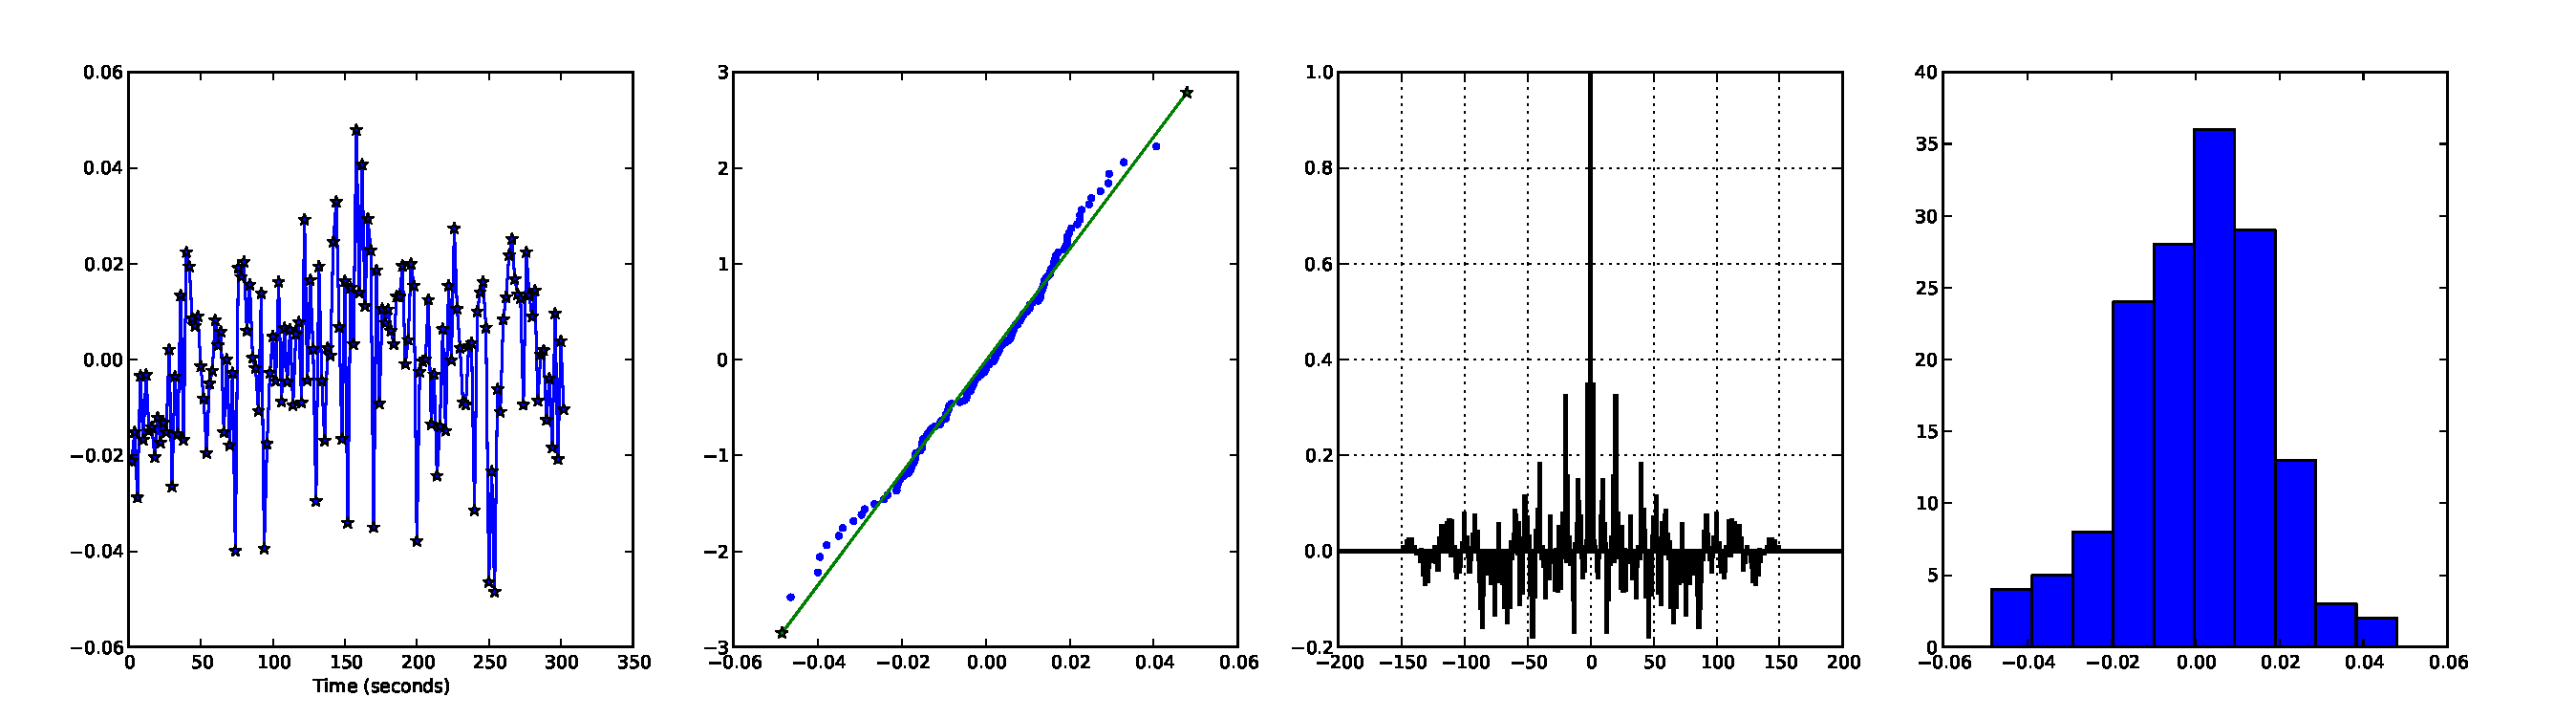
\includegraphics[trim=6cm 1cm 6cm 1cm,width=13cm]{images/noise2_0009_29_49_9}}
\subfigure[]{\label{fig:QQDC:B}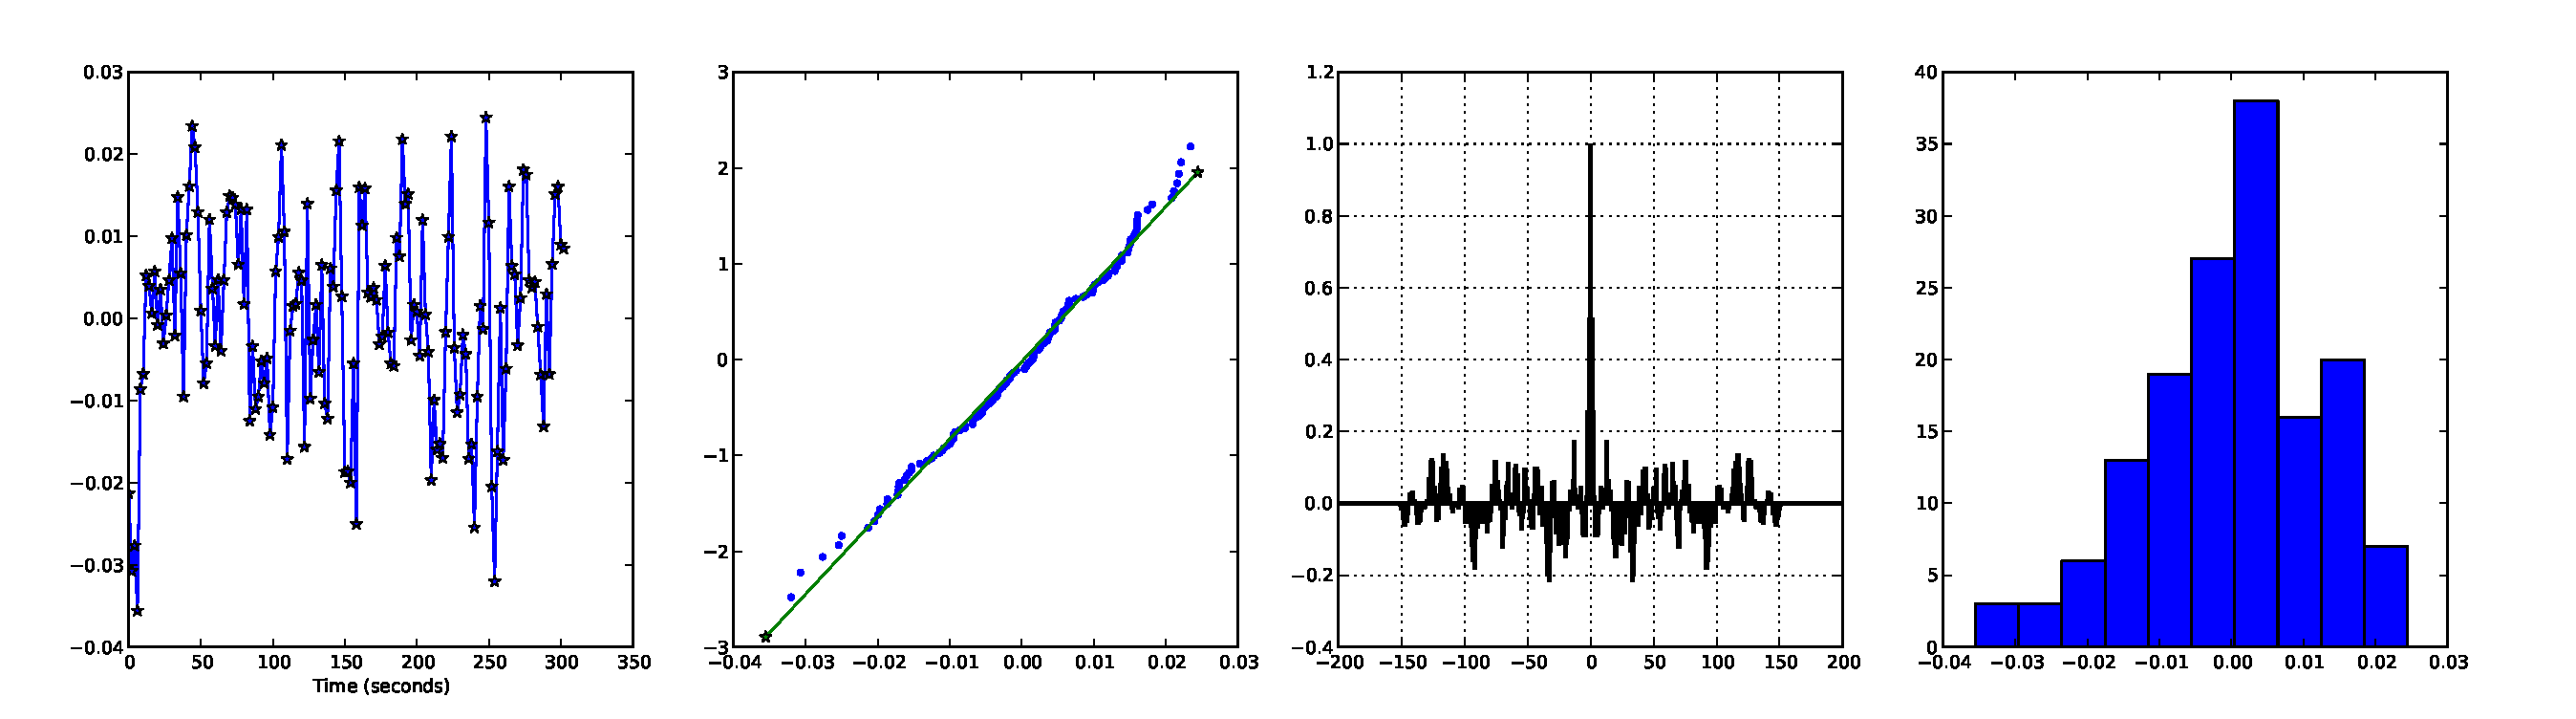
\includegraphics[trim=6cm 1cm 6cm 1cm,width=13cm]{images/noise2_0009_34_43_24}}
\subfigure[]{\label{fig:QQDC:C}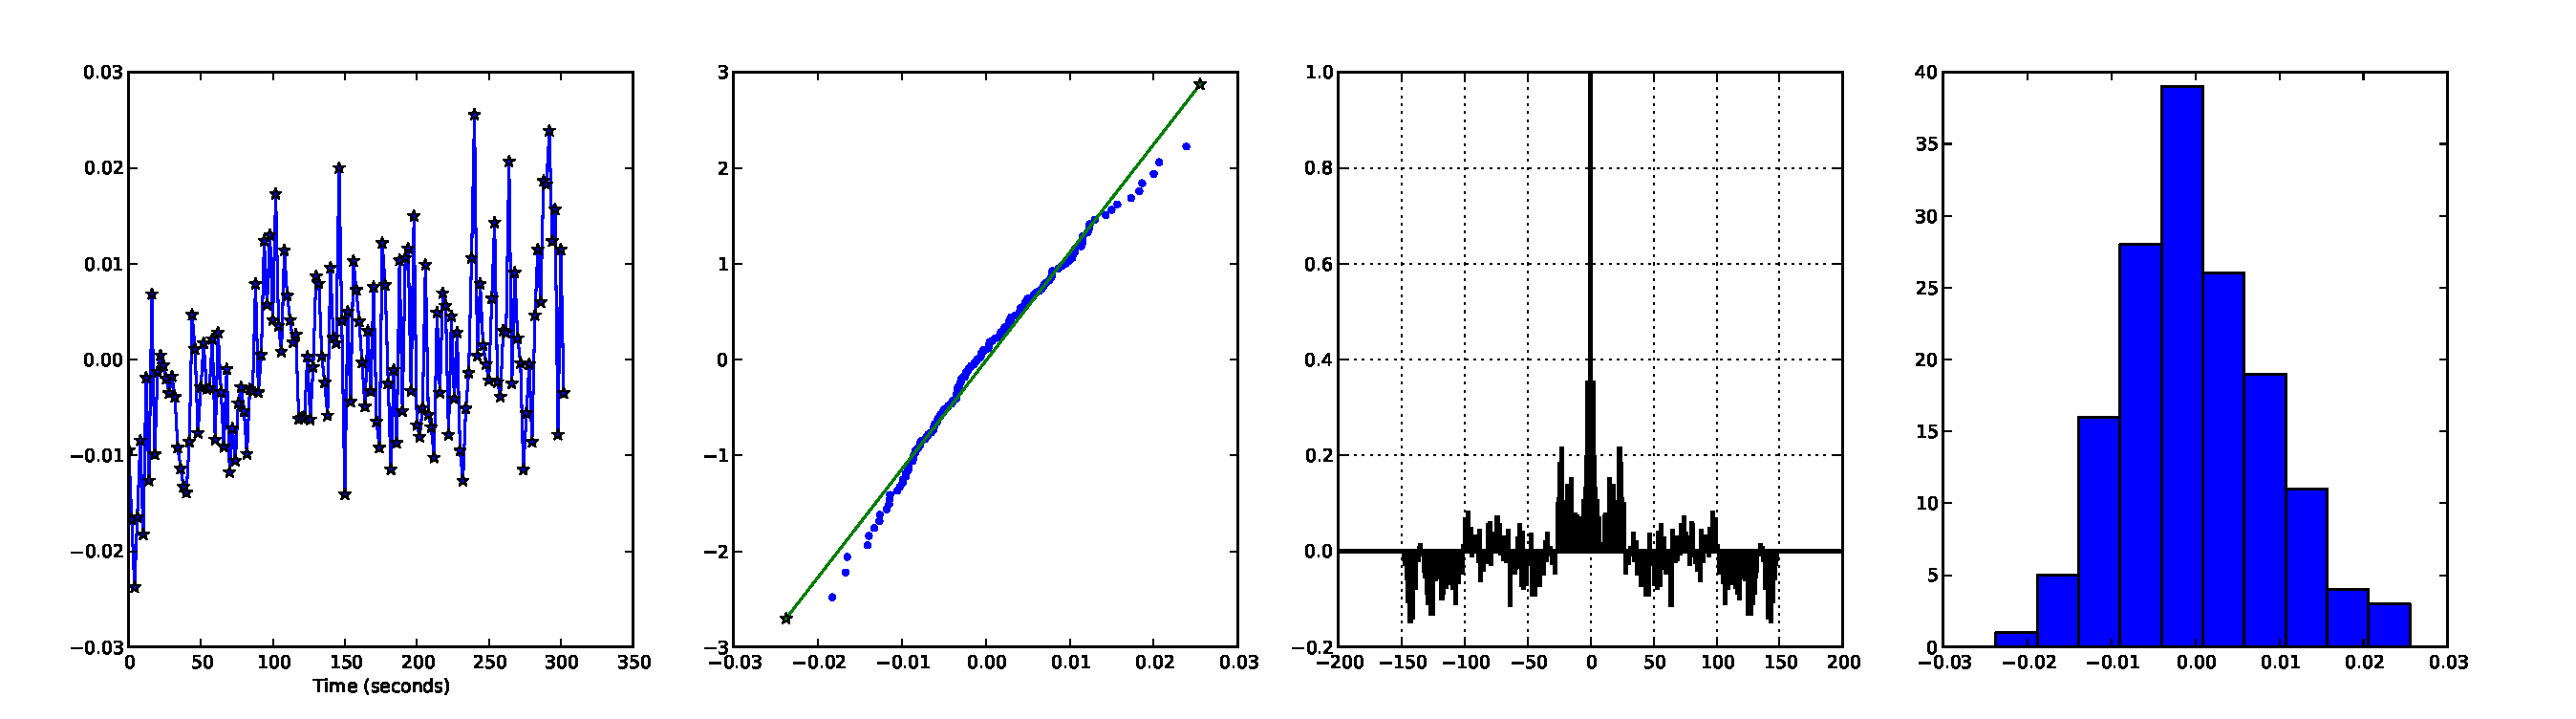
\includegraphics[trim=6cm 1cm 6cm 1cm,width=13cm]{images/noise2_0009_22_38_23}}
\subfigure[]{\label{fig:QQDC:D}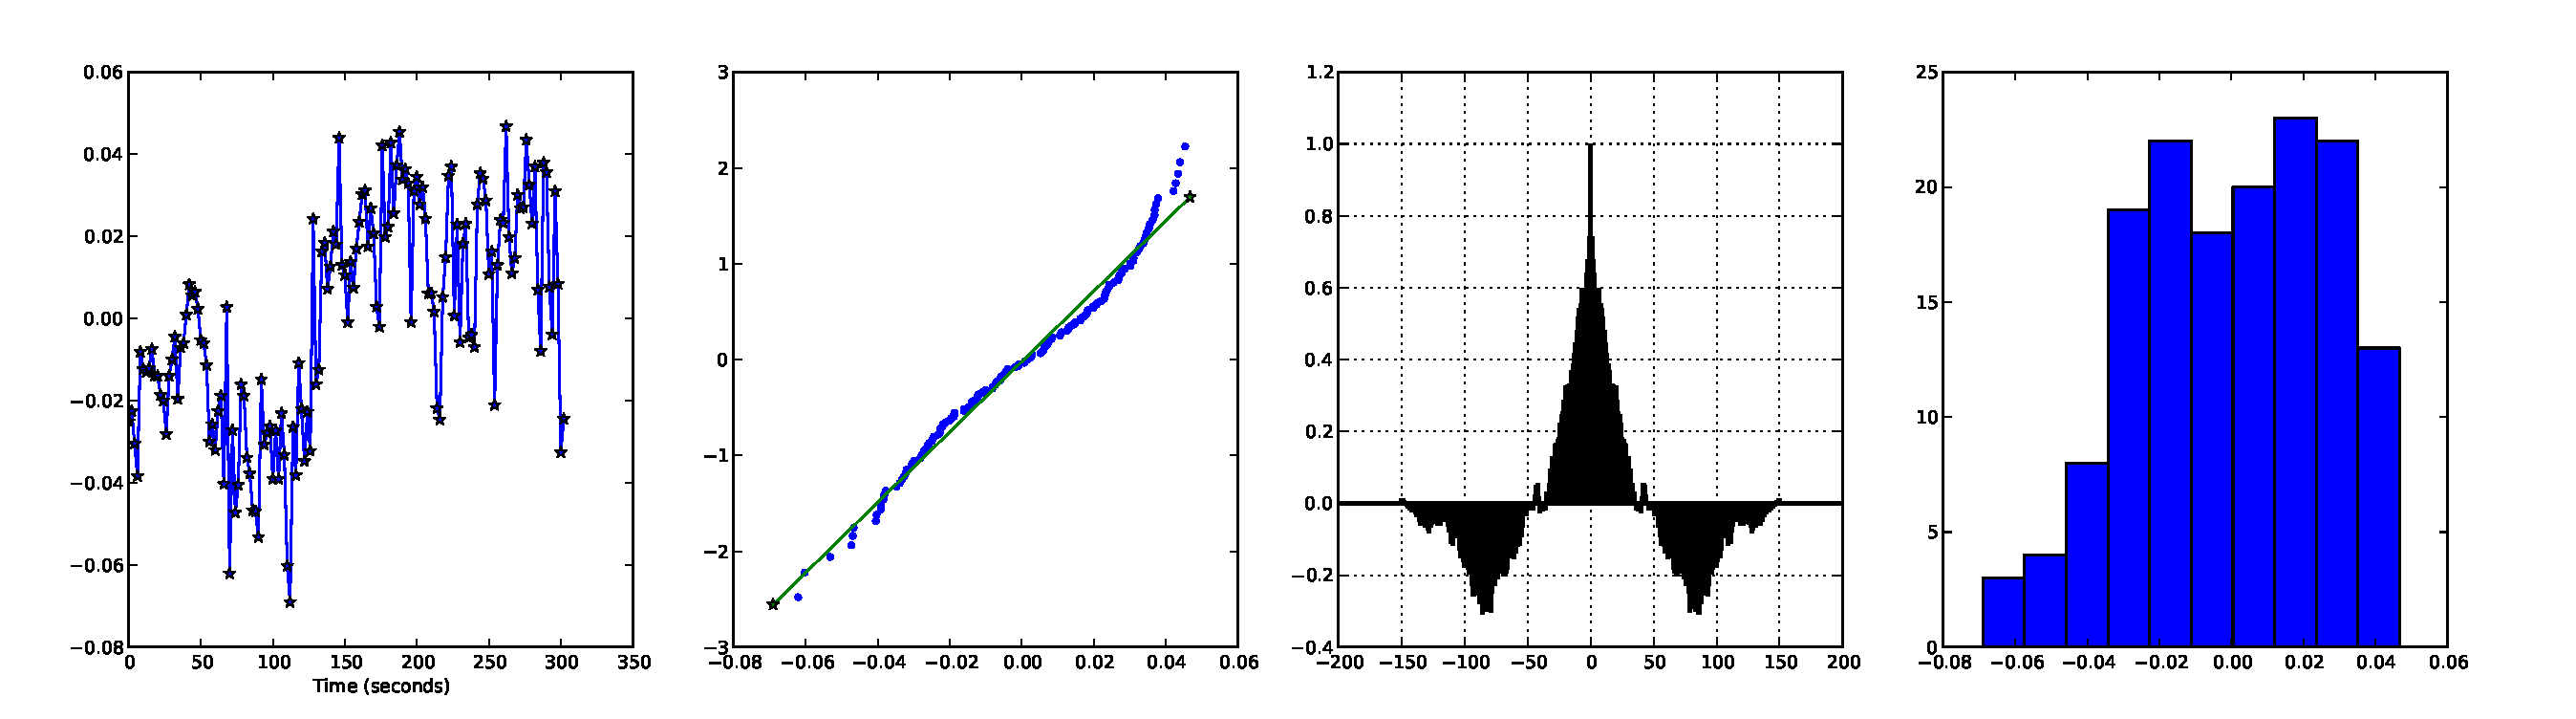
\includegraphics[trim=6cm 1cm 6cm 1cm,width=13cm]{images/noise2_0009_37_29_24}}

%\subfigure{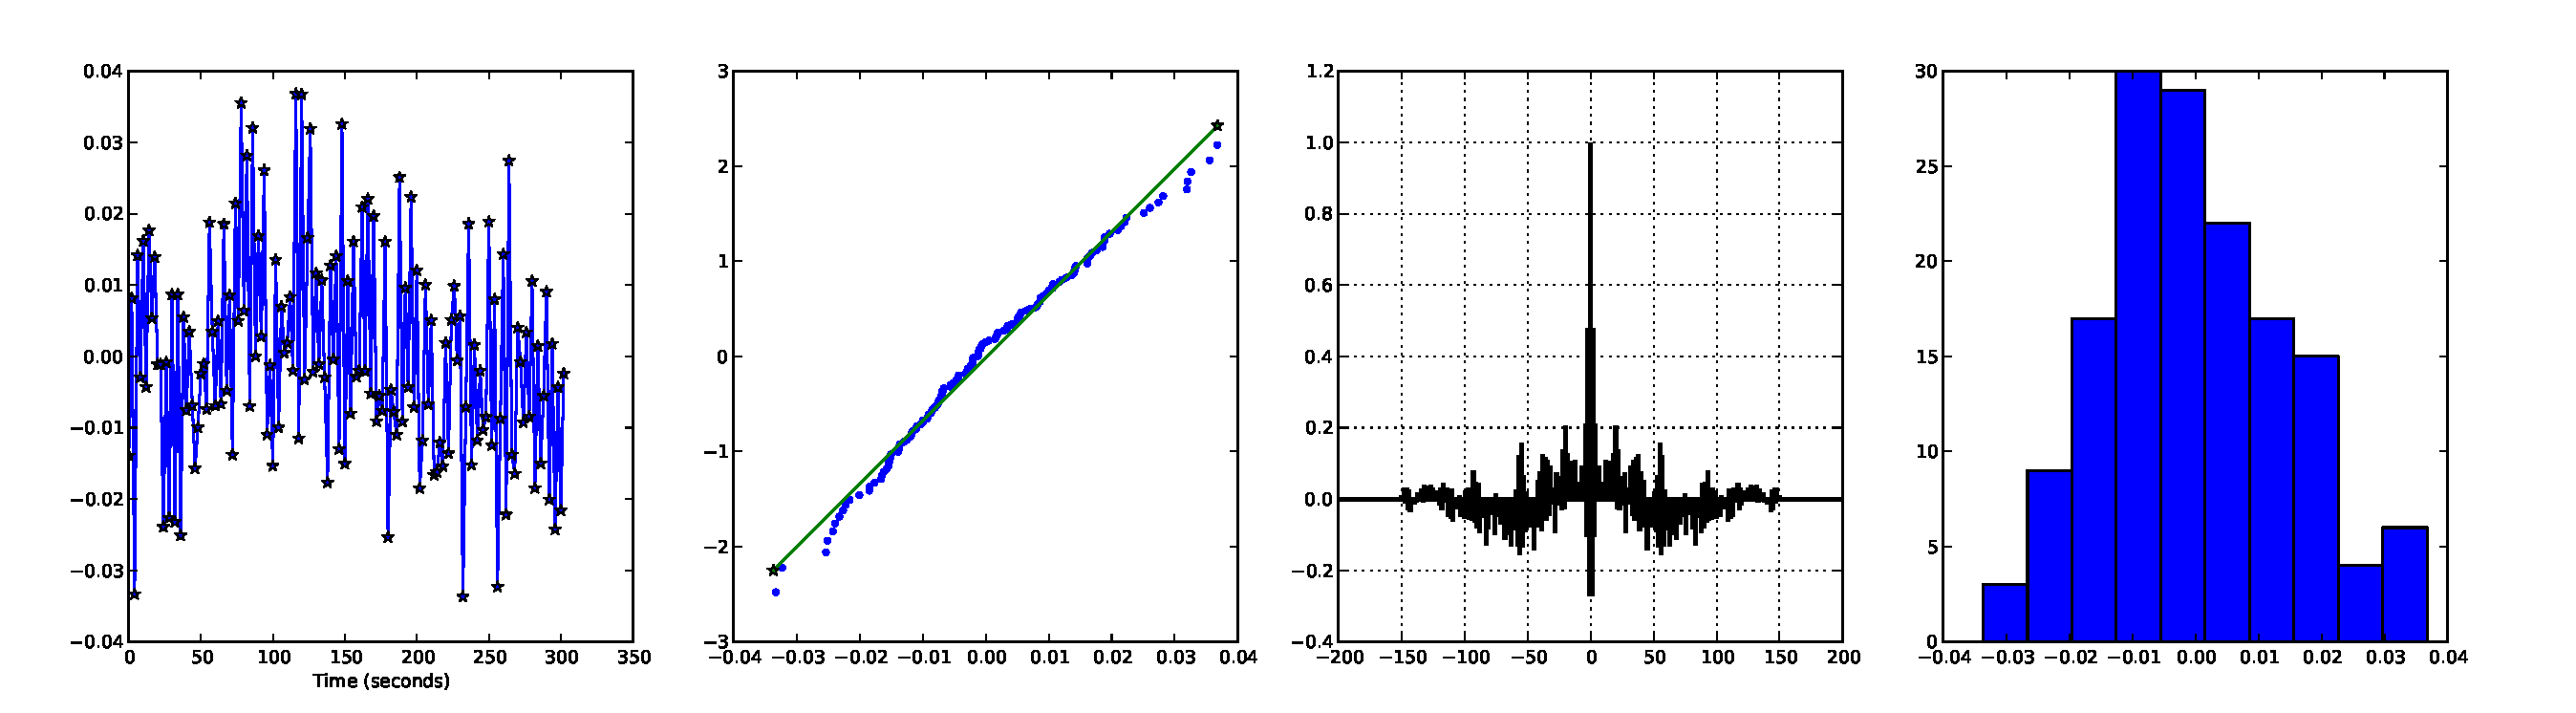
\includegraphics[trim=6cm 1cm 0 0cm,width=17cm]{images/noise_0009_19-24-10.pdf}}
%\subfigure{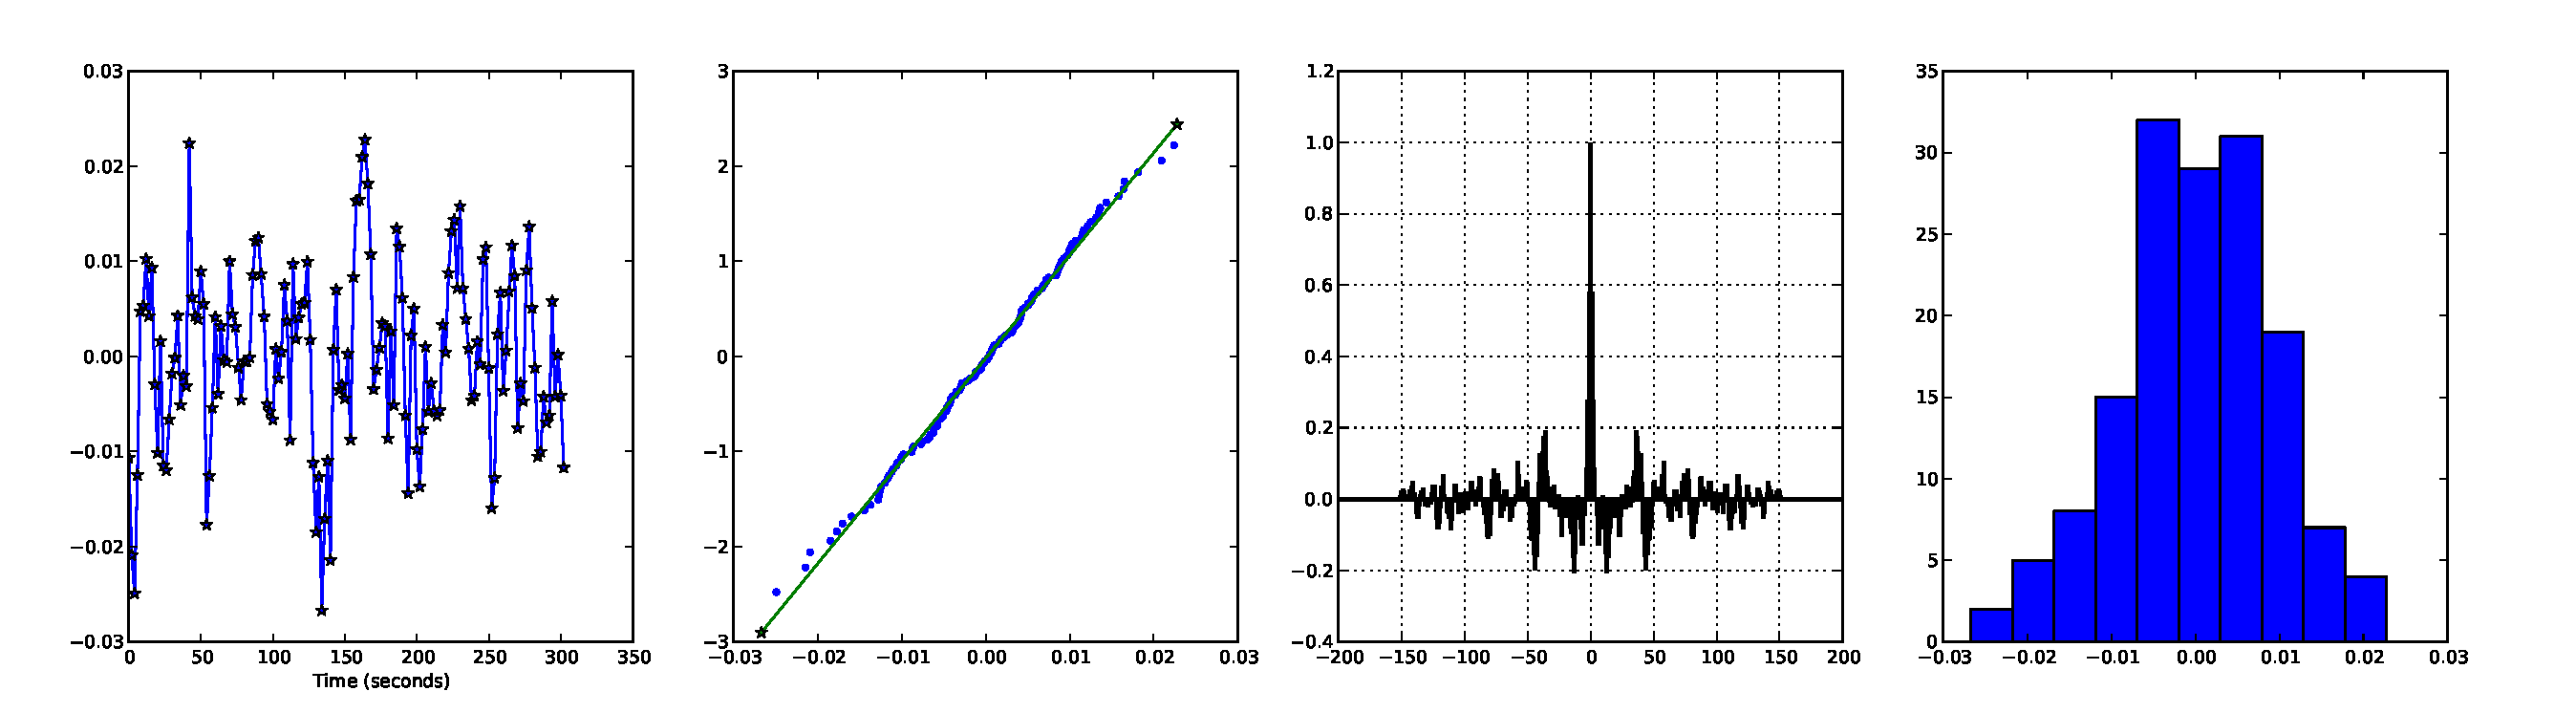
\includegraphics[trim=6cm 1cm 0 0cm,width=17cm]{images/noise_0009_20-45-18.pdf}}
%\subfigure{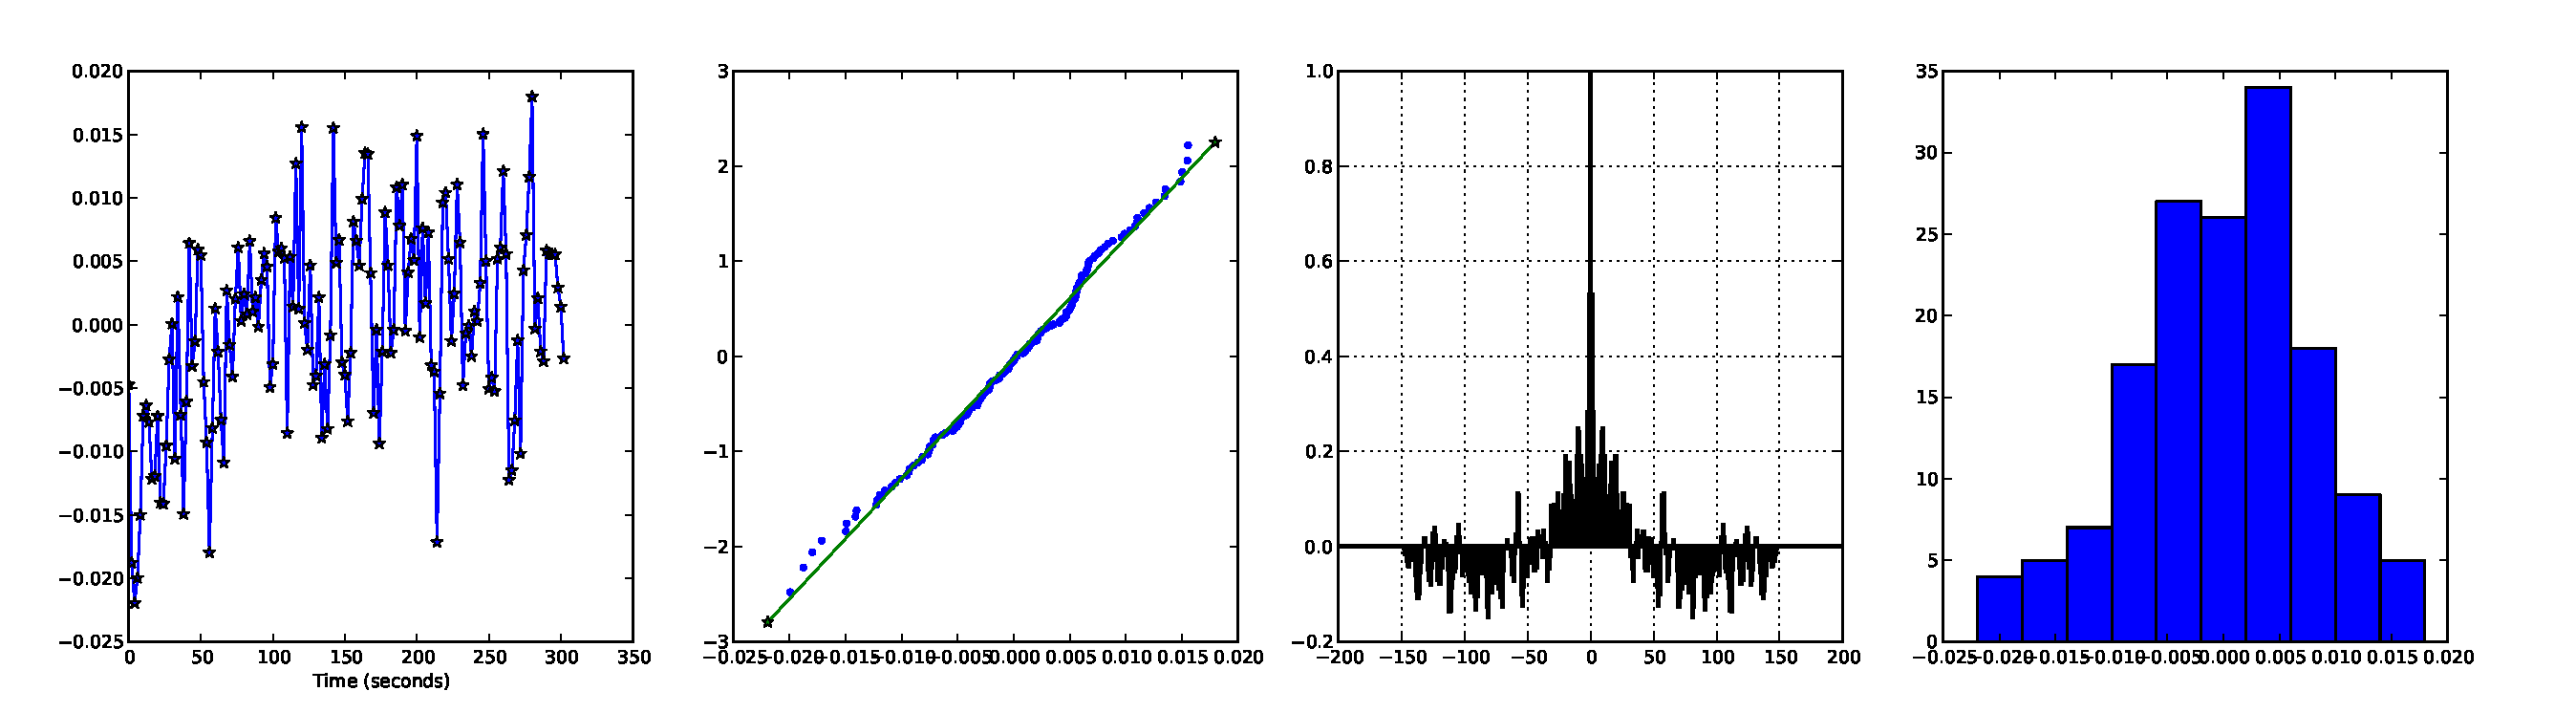
\includegraphics[trim=6cm 1cm 0 0cm,width=17cm]{images/noise_0009_23-47-18.pdf}}
%\subfigure{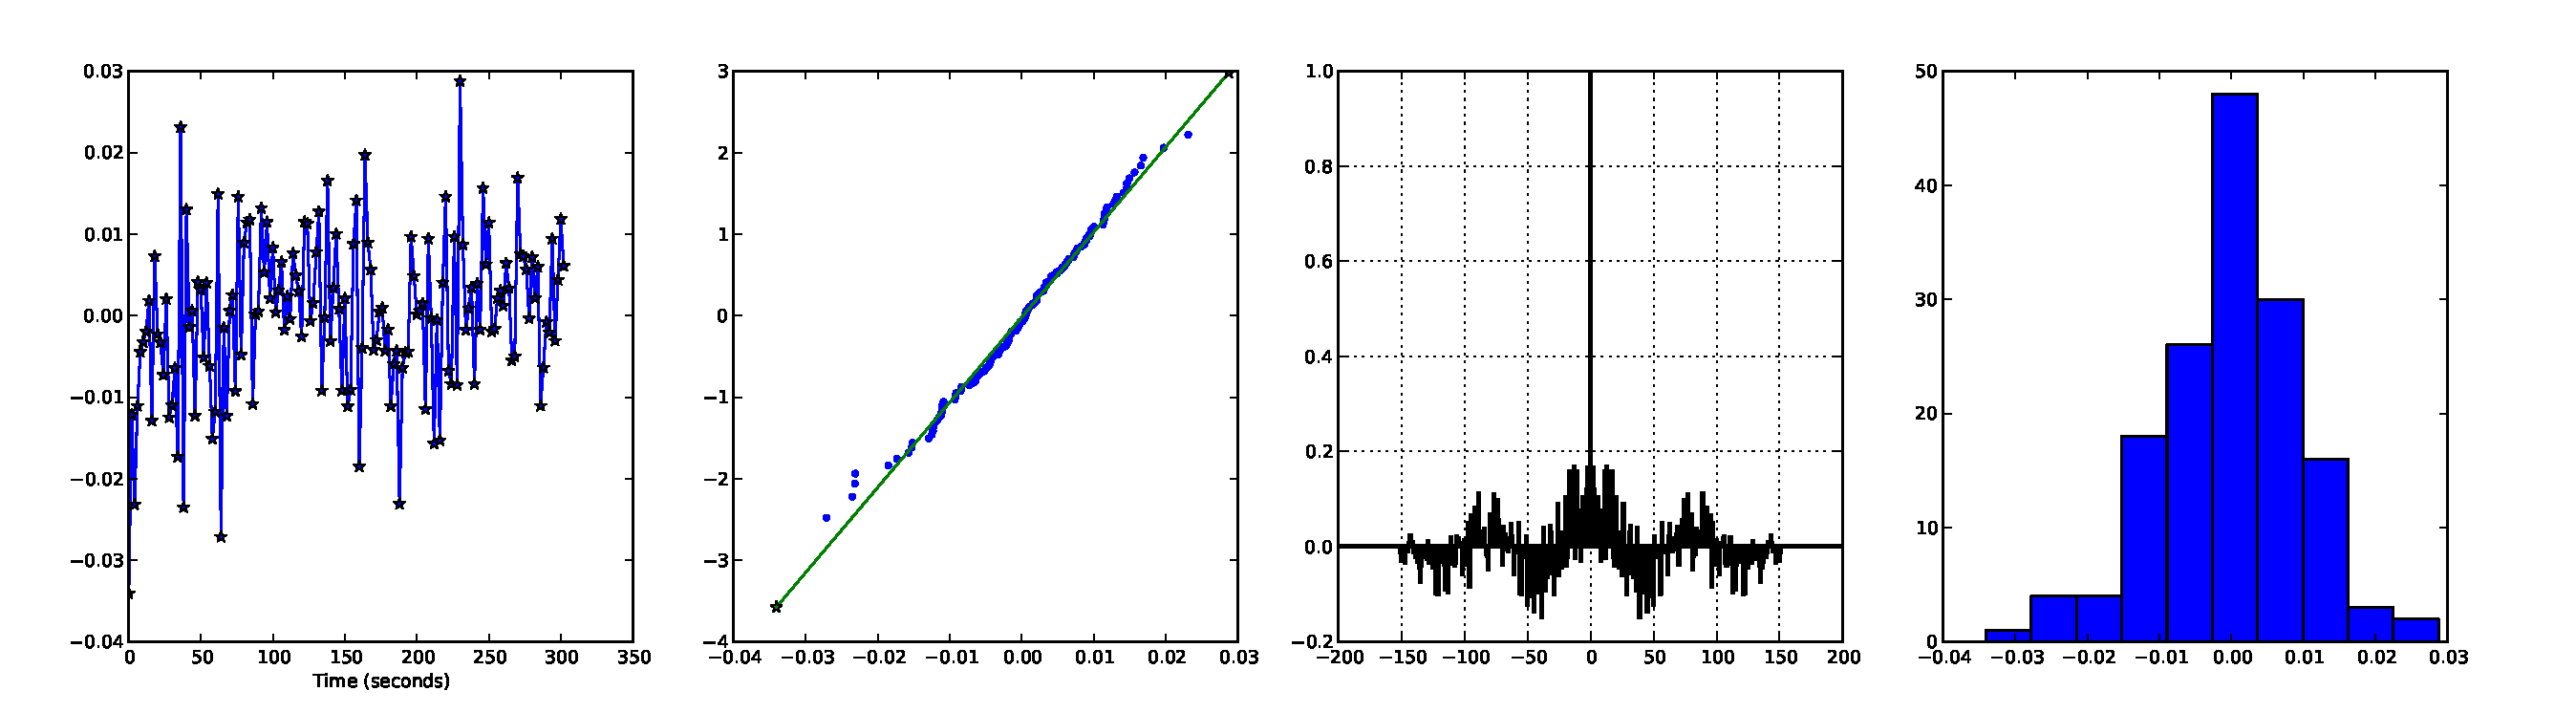
\includegraphics[trim=6cm 1cm 0 0cm,width=17cm]{images/noise_0009_35-49-9.pdf}}

\caption{Q-Q Plots of normalized resting state data}
\label{fig:QQDC}
\end{figure}

\begin{figure}
\centering
\subfigure[]{\label{fig:QQDDelta:A}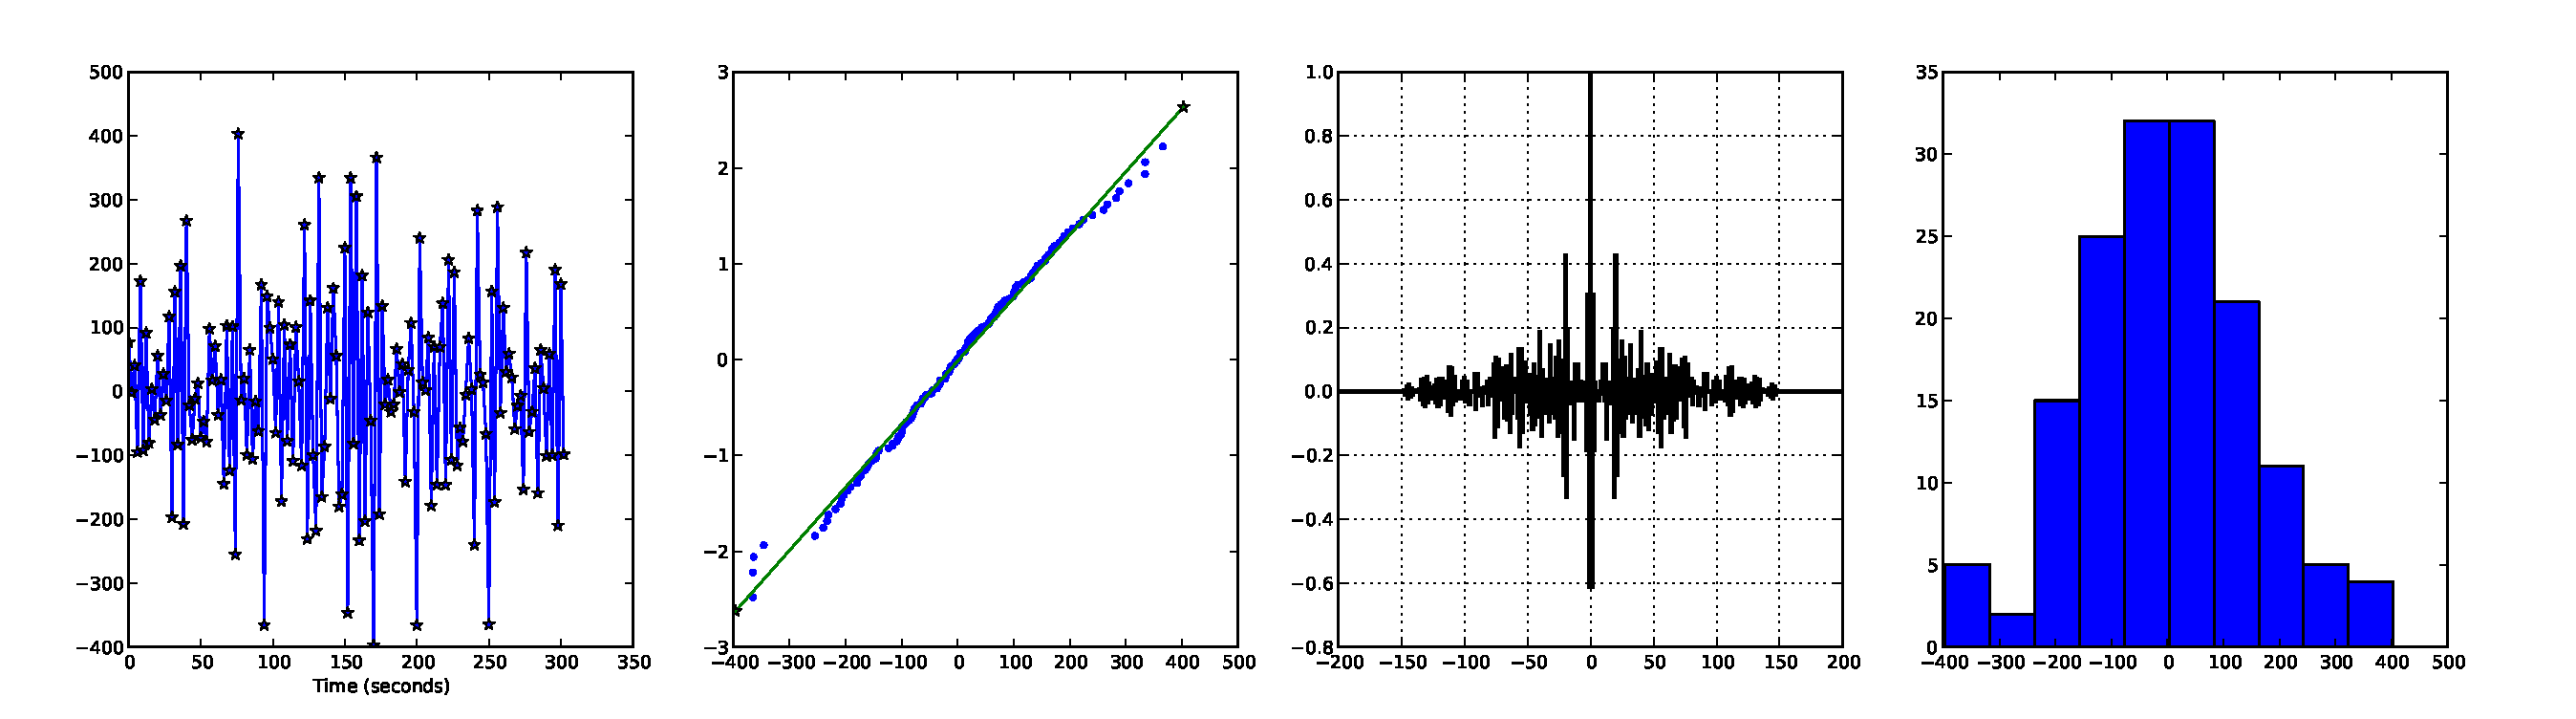
\includegraphics[trim=6cm 1cm 6cm 1cm,width=13cm]{images/noise2_0009d_29_49_9}}
\subfigure[]{\label{fig:QQDDelta:B}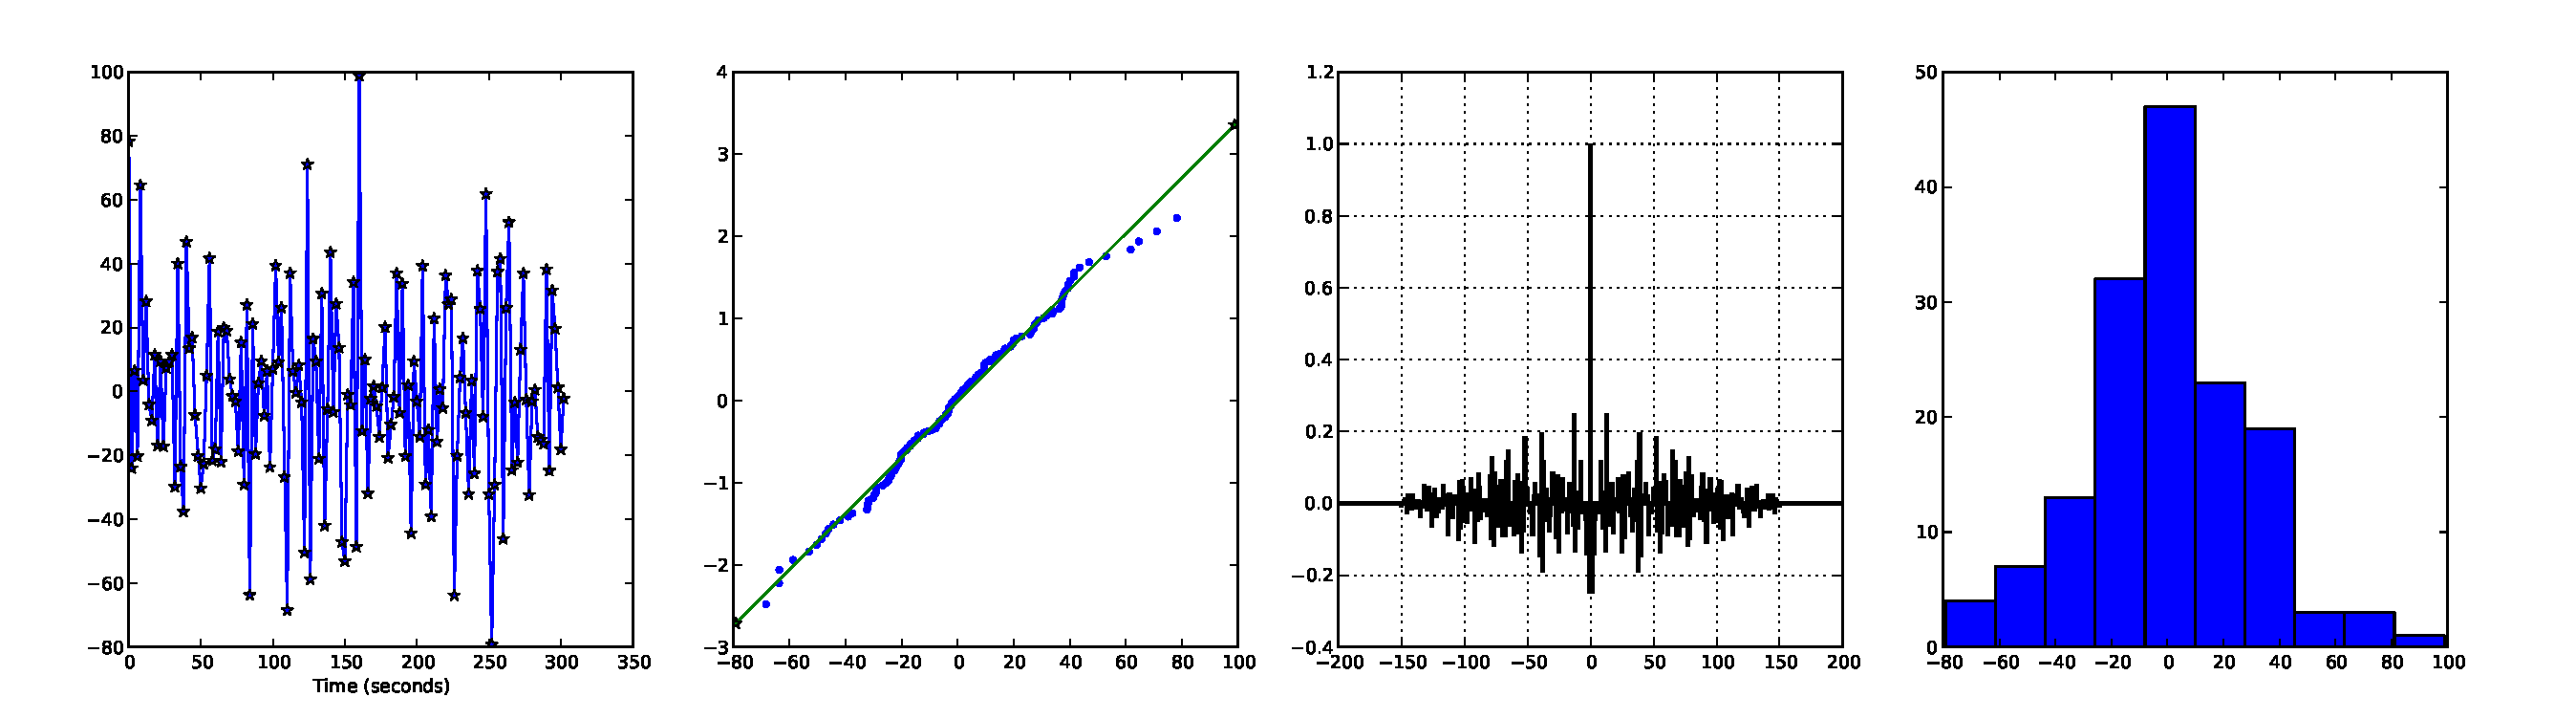
\includegraphics[trim=6cm 1cm 6cm 1cm,width=13cm]{images/noise2_0009d_34_43_24}}
\subfigure[]{\label{fig:QQDDelta:C}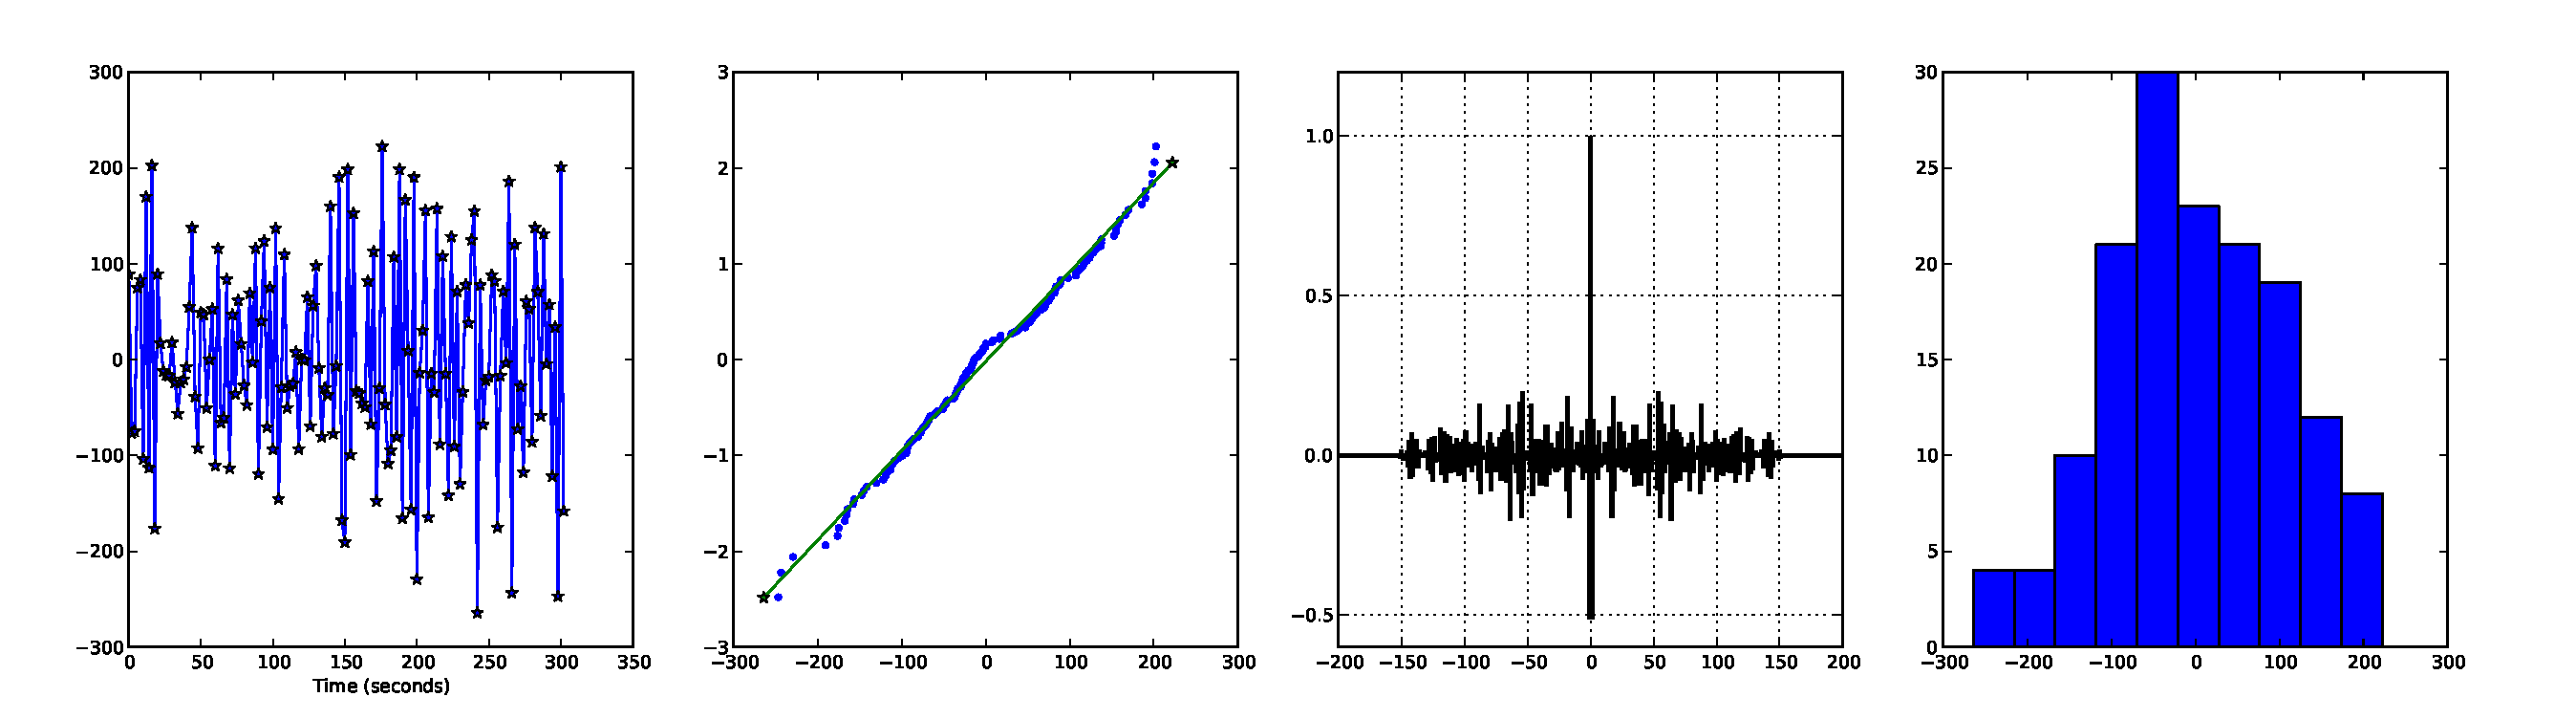
\includegraphics[trim=6cm 1cm 6cm 1cm,width=13cm]{images/noise2_0009d_22_38_23}}
\subfigure[]{\label{fig:QQDDelta:D}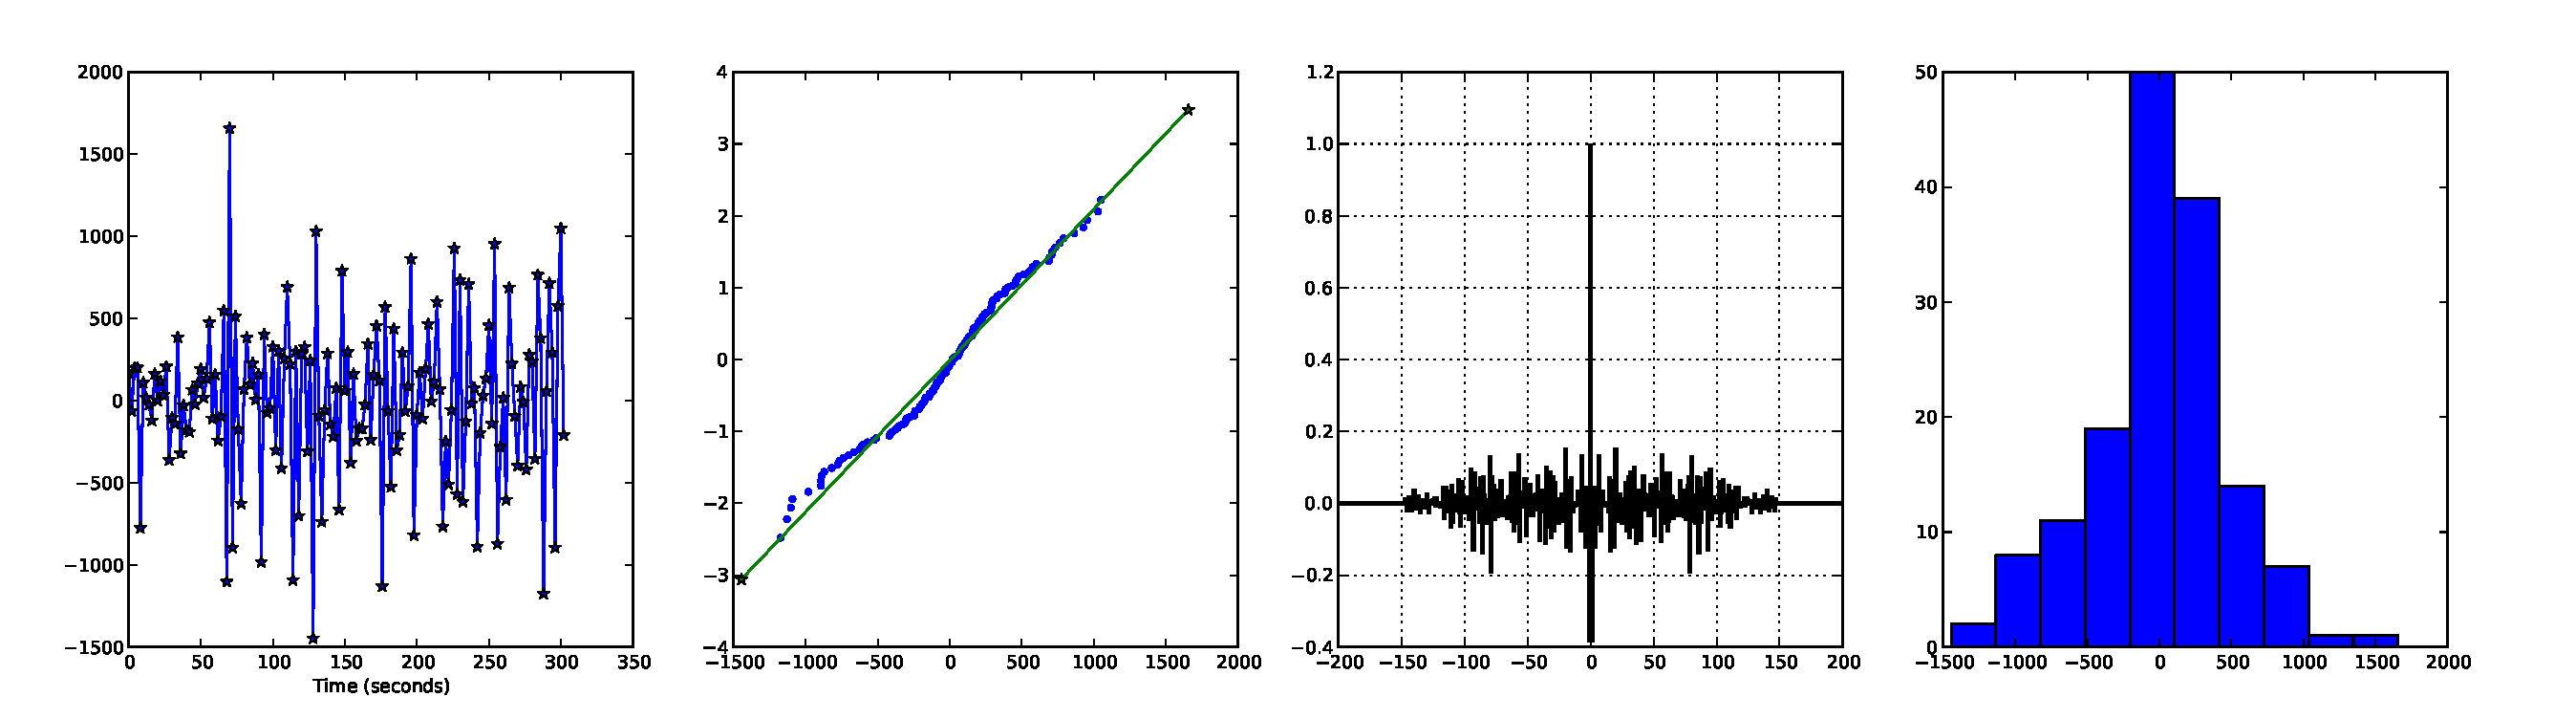
\includegraphics[trim=6cm 1cm 6cm 1cm,width=13cm]{images/noise2_0009d_37_29_24}}
\caption{Q-Q Plots of resting state data, using the BOLD signal changes}
\label{fig:QQDelta}
\end{figure}


\begin{figure}
\centering
\subfigure[]{\label{fig:QQs:A}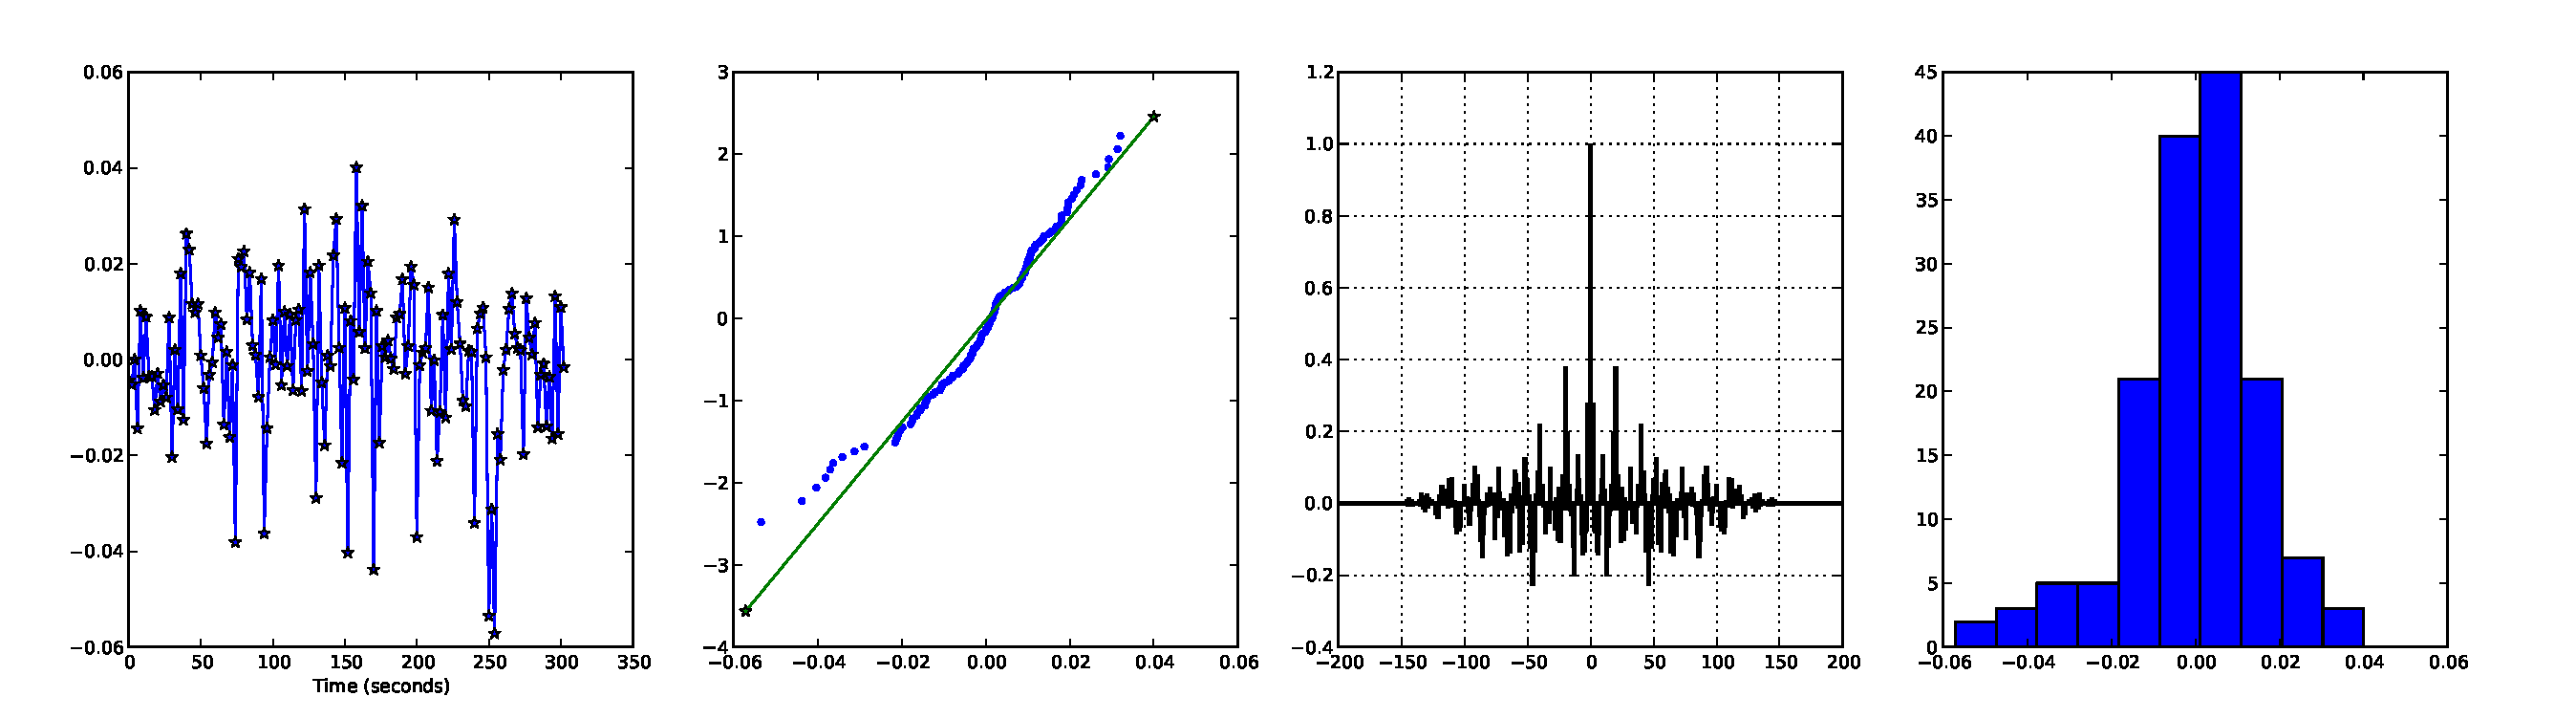
\includegraphics[trim=6cm 1cm 6cm 1cm,width=13cm]{images/noise2_0009s_29_49_9}}
\subfigure[]{\label{fig:QQs:B}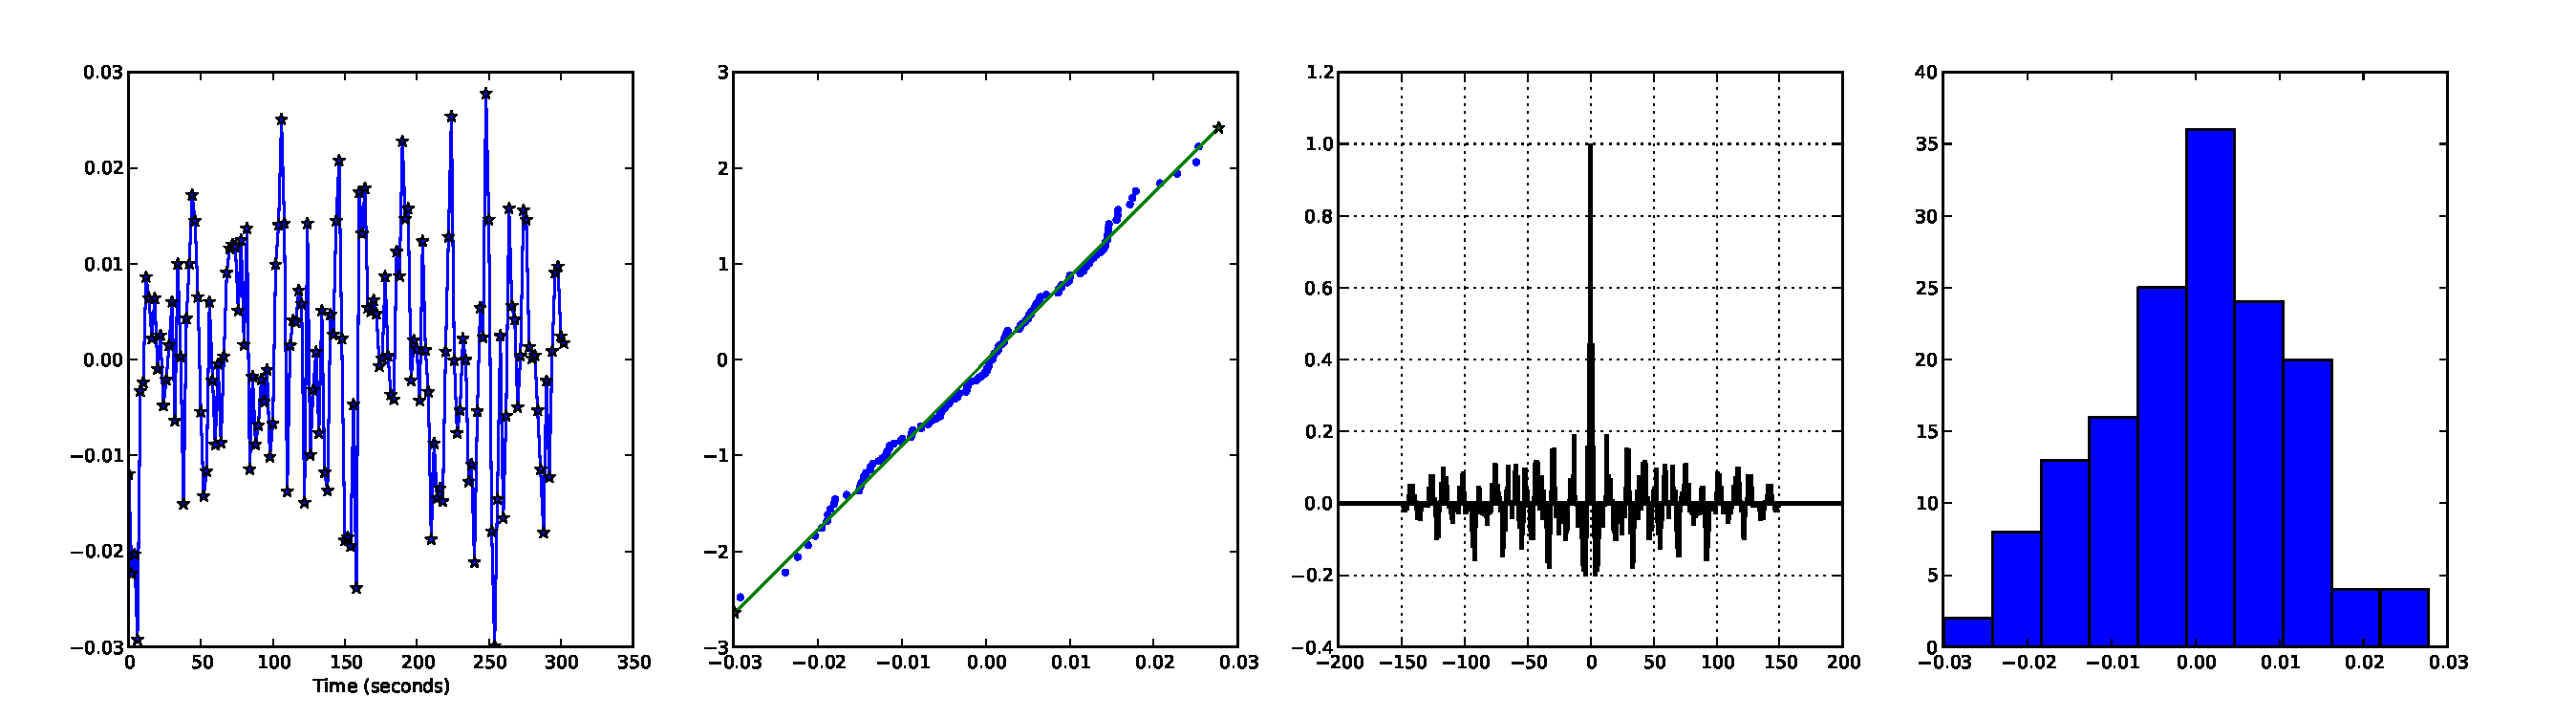
\includegraphics[trim=6cm 1cm 6cm 1cm,width=13cm]{images/noise2_0009s_34_43_24}}
\subfigure[]{\label{fig:QQs:C}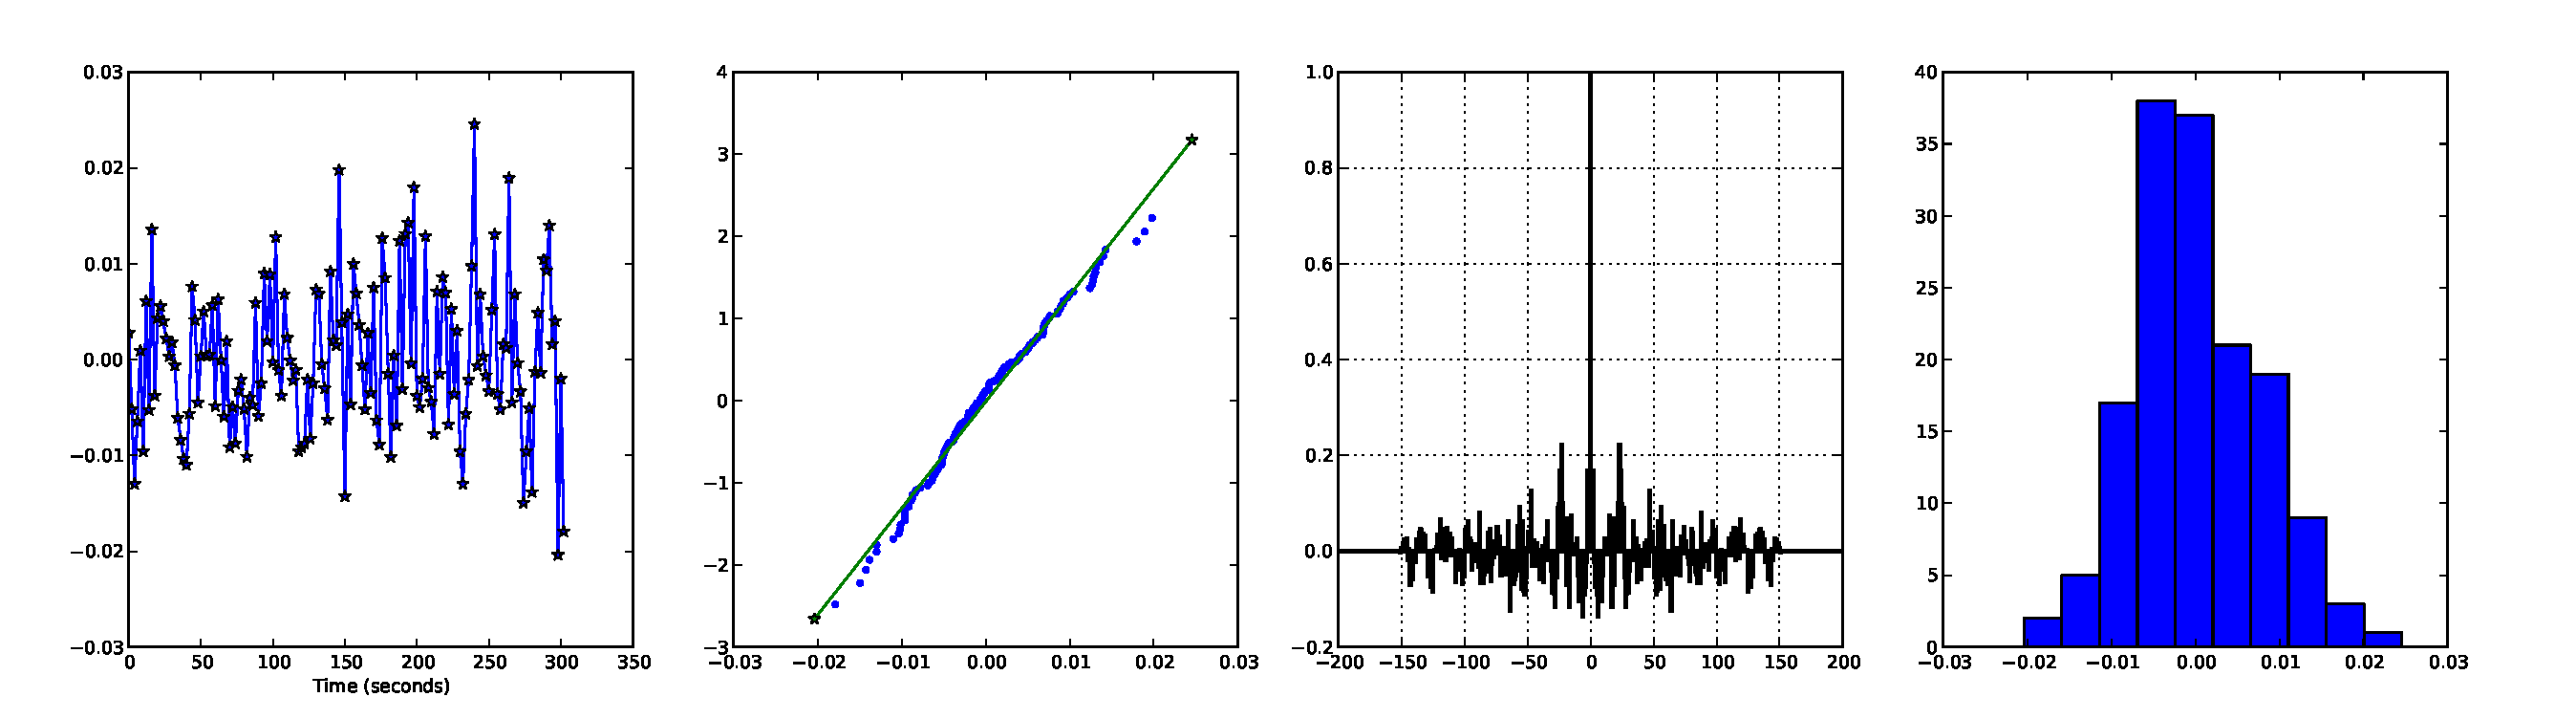
\includegraphics[trim=6cm 1cm 6cm 1cm,width=13cm]{images/noise2_0009s_22_38_23}}
\subfigure[]{\label{fig:QQs:D}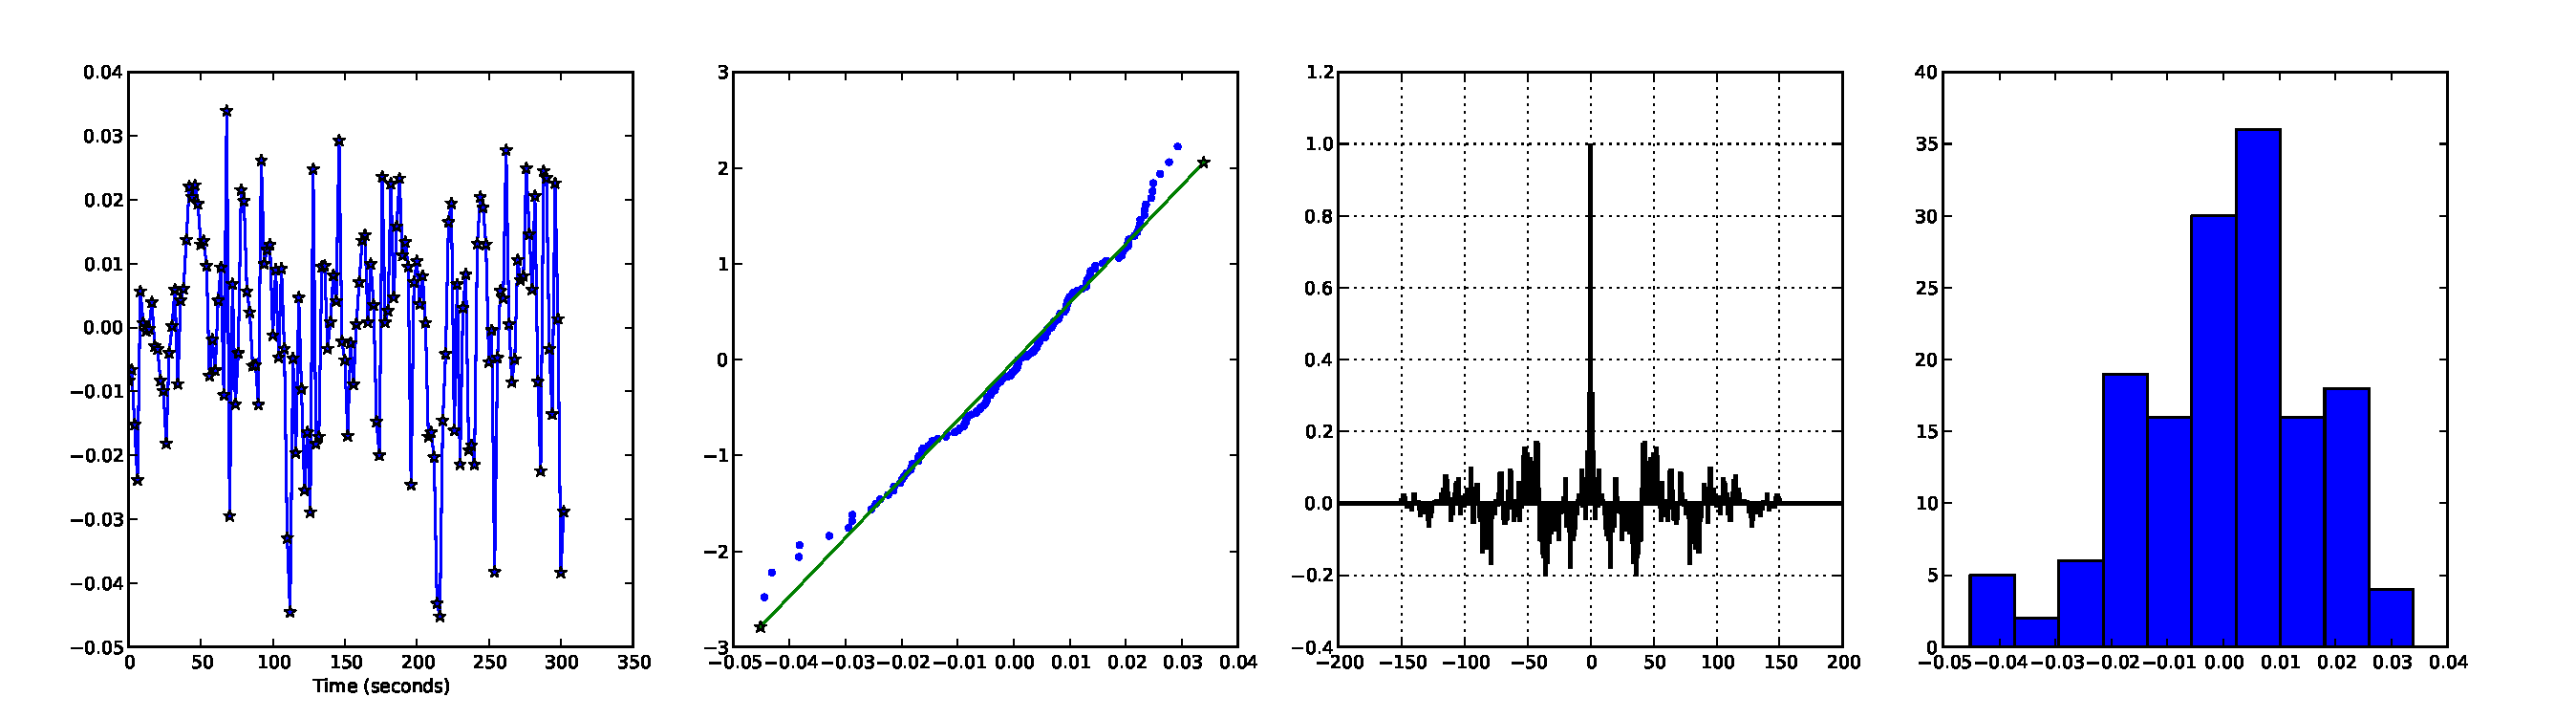
\includegraphics[trim=6cm 1cm 6cm 1cm,width=13cm]{images/noise2_0009s_37_29_24}}
\caption{Q-Q Plots of resting state data, after the de-trending}
\label{fig:QQSpline}
\end{figure}

Because most methods (including the one used in this paper)
assume the noise realizations are independent of each other, the auto-
correlation is of particular interest (which is a necessary but not
sufficient condition for independence). Gaussianity is also a common
assumption made in studies of FMRI data, though that assumption is not
needed in this work. Regardless, comparing the distribution to a Gaussian
is informative, so Q-Q plots are used to compare example data with the
Normal distribution. Additionally, in FMRI data the noise is often considered 
to be Wiener \cite{Riera2003}. Recall that a Wiener random process is
characterized by steps that are Gaussian and independent. The simulations discussed in 
\autoref{sec:Single Voxel Simulation} make use of this, 
by adding a Wiener random process to the overall signal. To determine
whether the noise is in fact Wiener, the distribution of 
the steps were plotted against a Gaussian. 

Finally, removal of the drift is often performed with a high pass filter,
so analyzed the distribution after subtracting of a spline, (see \autoref{sec:Methods Preprocessing}).

\autoref{fig:QQDC} shows the 
results with a regression line fit to the points.
Recall that in a Quartile-Quartile (Q-Q) plot, if the points plotted on the 
x-axis and the points
on the y-axis come from the same type of distribution, then all the points will
be collinear. Differences in the variance will cause the line to have a slope
other than 1, while differences in the expected value will cause the fitted line
to be shifted. In these Q-Q plots, the points are being compared to the standard
Gaussian distribution. Note that in \autoref{fig:QQDC} the points have all been 
normalized (changed to percent difference).

Note that \autoref{fig:QQDC:A} and \autoref{fig:QQDC:B}
are well described by a Gaussian process with a small autocorrelation, 
\autoref{fig:QQDC:C} and \autoref{fig:QQDC:D} are not. In particular the tails of \autoref{fig:QQDC:C}
do not seem to fit the Gaussian well. Also note the significant autocorrelation in
\autoref{fig:QQDC:C} and \autoref{fig:QQDC:D}. As expected, the noise is not strictly
Gaussian white noise.  On the other hand, the steps do conform rather
closely to the normal distribution.
As expected, most of the autocorrelation disappears for the step data. Given
that the steps seem to fit the Normal distribution, the low autocorrelation
indicates that the steps could be Independently Distributed. 
Therefore, the noise does seem to come close to a Wiener process. 

De-trending the time-series by subtracting a spline fit to the distribution
removed much of the autocorrelation present in \autoref{fig:QQDC:C} and \autoref{fig:QQDC:D},
though not perfectly. Though the distributions still do not exactly fit
the Normal, \autoref{fig:QQs:D} is much improved compared to \autoref{fig:QQDC:D}.
In all, the de-trending is effectively removing Wiener noise. 

\subsection{Detrending}
\label{sec:Detrend}
The non-stationary
aspect of a Weiner process, presumably the result of integrating some
$\nu_x$ is difficult to compensate for, and so many methods
have been developed to compensate for it. \cite{Tanabe2002} and \cite{Smith1999} have
demonstrated that this component is prevalent, and may in fact be an inherent  characteristic
of FMRI. It has been reported that in some studies as many as half the voxels 
benefited from detrending (\cite{Smith2007}). In a head to head comparison, 
\cite{Tanabe2002}, showed that in most cases subtracting off
a spline worked the best. The benefit of the spline versus wavelets, high pass 
filtering or other DC removal techniques is that the frequency response is not set.
Rather, the spline is adaptive to the input. Unfortunately no method will 
perfectly remove noise, and no method will leave the signal untouched.

The method I used to calculate the spline was picking one knot for every 20
measurements in an image. Thus a 10 minute session at a repetition time of 
2.1 seconds would have 19 knots. The knot first and last knots were each 
given half the number of samples as the rest of the knots; which were all 
located at the center of their sample group. The median of each sample group
was then taken and used as the magnitude for the group. Taking the median 
versus the mean seemed to work better, given the presence of outliers. 
There is potential to optimize the spline further using a canonical 
HRF to find resting points; however, for this to work the experiment would have
to be designed with this in mind. 

Problematically, after removing the DC component of the signal,
by definition the signal will have a median near zero. 
Unfortunately this is not the natural state of the BOLD signal. More specifically,
when the signal is inactive, the BOLD response should be at 0\% change from
the base level; activation may then increase, or for short periods decrease from this base.
Because most of the BOLD signal is above baseline, after removing the spline
the BOLD resting state will be below 0\%.  This reduces the ability of an algorithm to learn.
One method of accounting for this is to simply add a DC gain model parameter.
Like all the other model parameters, with enough measurements, a viable
parameter would fall. Yet adding another dimension increases the
complexity of the model, when the parameter is relatively easy to estimate
by visual inspection.  In this work a simpler approach was used. To determine
the DC gain I used a robust estimator of scale. The Median Absolute Deviation (MAD)
proved to be accurate in determining how much to shift the signal up
by. I tested both methods during the course of analysis, and found that the increase 
in model complexity far outweighed the slight increase in flexibility. Other
methods may work better, however the MAD worked well, 
as \autoref{fig:PreprocessedLowNoise} and \autoref{fig:PreprocessedHighNoise} show. 

\begin{equation}
y_{\text{gain}, 0:K} = 1.4826\text{median}_{i=0:K}(y_i - \text{median}(y_{0:K}))
\end{equation}

A serious concern when adding and subtracting arbitrary values to 
real data is whether this will create false positives. This is a legitimate
concern; however, a boosted response does not effect how well the BOLD model 
predicts the actual measurements. 

%\subsection{Linearizing Noise}
%\label{sec:Methods Delta Based Inference}
%The alternative to these sorts of low frequency manipulation is to
%go around the problem in another way. Here, I propose a 
%different method of dealing with the drift. 
%Instead of comparing the direct output of the particle filter with the direct
%measurement, the algorithm would compare the change in signal over a single TR,
%with the result of integrating the model for the same period. 
%In most signal processing cases this would be foolish, but that is because the 
%general assumption is that all noise is high frequency. Considering 
%the fact that every BOLD analysis pipeline uses a high pass filter,
%whereas low poss temporal filter are rarely applied, it makes sense
%that a derivative type method could work. The benefit of particle filters
%is that they are a robust method of inference, and I would assert 
%that the particle filter ought to be given as \emph{raw} data as possible. 
%While taking direct measurements
%without de-trending would give awful results, using the difference removes the 
%DC component and turns what is usually assumed to be a Weiner process into 
%a simple Gaussian random variable. 
%
%\begin{equation}
%\Delta y = y(t) - y(t-1) = g(x(t)) - g(x(t-1)) + \nu_y(t) - \nu_y(t-1) + \nu_d(t) - \nu(t-1)
%\label{eq:measass_delta}
%\end{equation}
%
%Even if $\nu_d$ is some other additive process, the difference will still be closer
%to I.I.D. than a Wiener process, as the autocorrelation of the $\delta y$ shows
%in \autoref{fig:QQDelta} in \autoref{sec:Introduction Noise}. 
% All the assumptions made originally
%for the particle filter still hold, and all of the parameters may be distinguished based on
%the step sizes, thus it is not unreasonable to consider matching the string of step sizes
%rather than string of direct readings. 
%
%\begin{figure}
%\label{fig:FrequencyGraphs}
%\caption{frequency response graphs, highlighting noise frequency range and signal frequency range}
%\end{figure}

\section{Particle Filter Settings}
There are quite a few options when using a particle filter; those
options will be discussed in this section.

\section{Prior Distribution}
\label{sec:PriorDist}
For the BOLD model described in \autoref{sec:BOLD Physiology}, several
different studies have endeavored to calculate parameters. The results
of these studies may be found in \autoref{tab:Params}, and the methods 
used for each may be found in \autoref{sec:Prior Works}. Unfortunately,
\cite{Friston2000} only studied regions deemed active by the General 
Linear Model; and most other research (including \cite{Friston2001}) used these results as 
the source for their priors. 
The one exception is \cite{Johnston2008}, which came to a extremely different
distributions. For a particle filter, the choice of a prior is
the single most important design choice. A very wide prior will require
more particles to be sufficiently dense, a very thin (low variance) prior may miss
the true parameters. Consequently, for this work it was natural
to use priors that will give results consistent with previous works, 
\cite{Friston2000}. This constrains the usefulness of the model to
areas that fall within the prior distribution, yet will allow results
to be comparable to other works. There is a significant need for better
estimates of the physiological parameters; and, while physical experiments
may not be possible, it would not be unreasonable to do a study with
exhaustive simulated annealing or hill climbing tests for multiple
regions and multiple patients.

There is an interesting anomaly with the priors found in virtually all
the works that characterized the parameters, except \cite{Johnston2008}.
The BOLD signal is universally recognized to be around $2-3\%$, maybe
reaching $5\%$ in extreme activation. Yet using the mean priors
from \cite{Friston2000}, the signal response for a $.1$ second
impulse only reaches maybe half a percent, as \autoref{fig:MeanResponseF}
shows.

\begin{figure}
\centering
\label{fig:MeanResponseF}
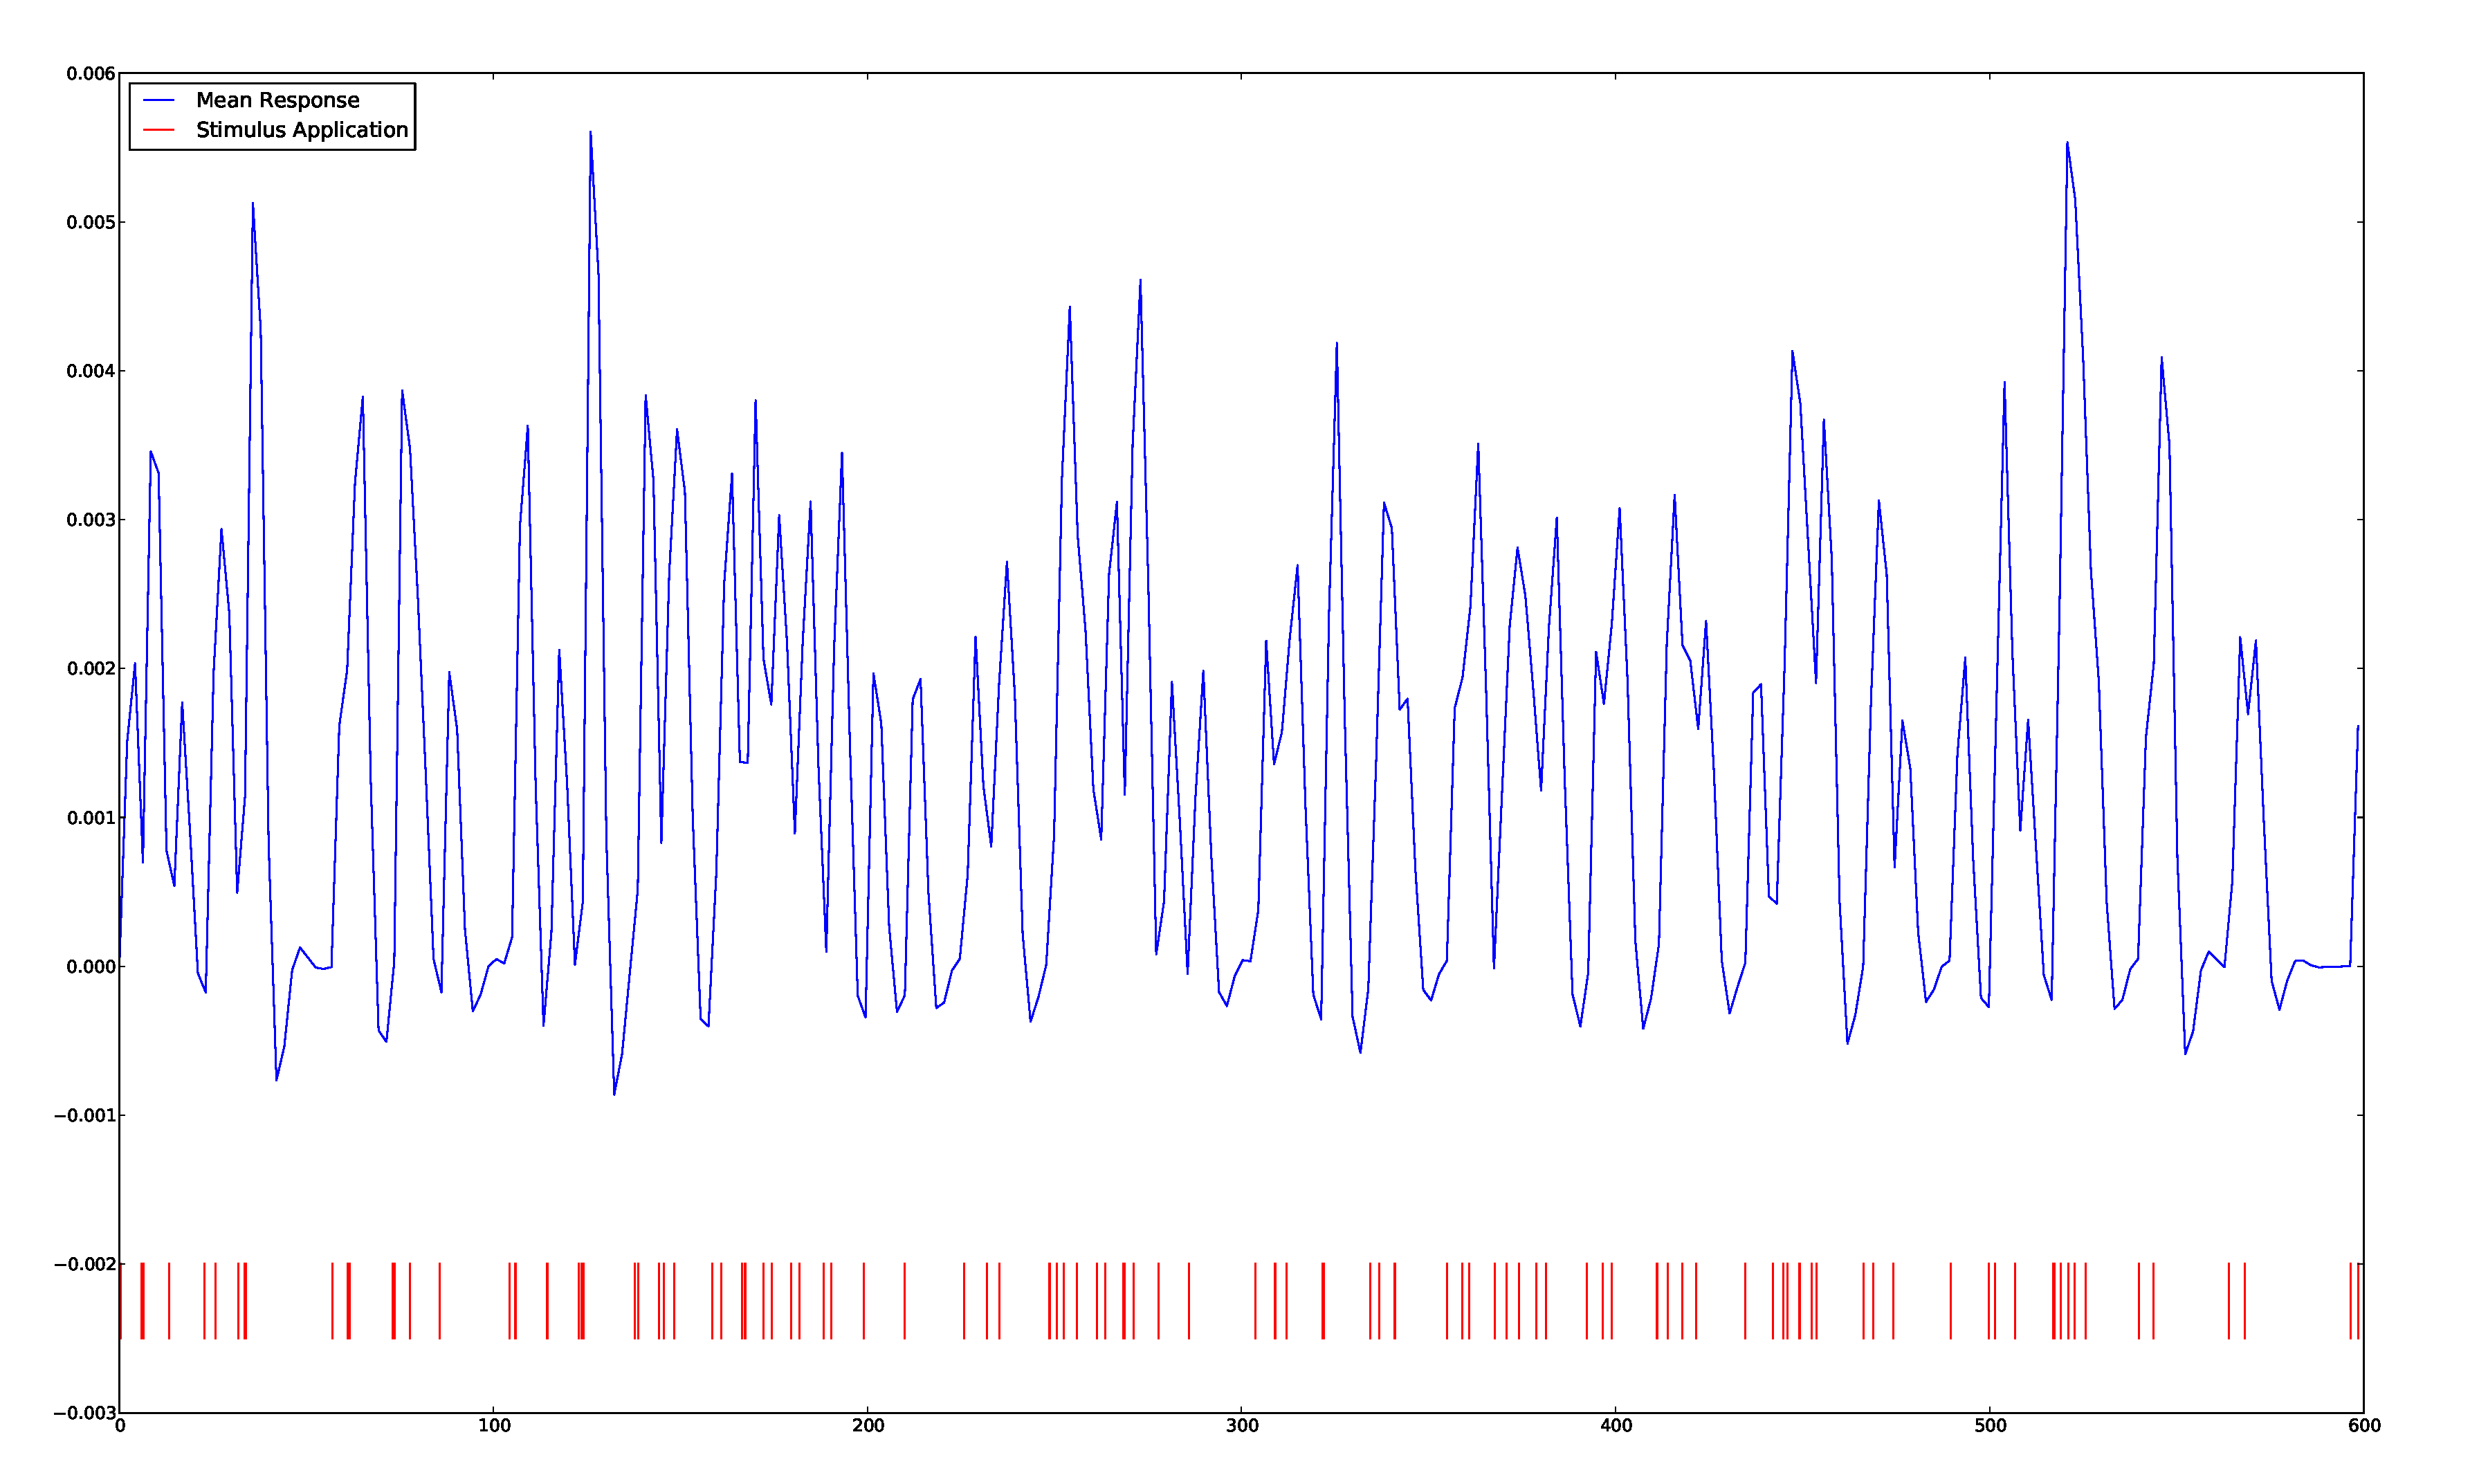
\includegraphics[trim=6cm 3cm 6cm 3cm,width=16cm]{images/mean_response}
\caption{Response to $.1s$ impulses with the mean parameters from \cite{Friston2000}}
\end{figure}

While this could be the result of a stimulus
being too short to lead to strong activation, a similar stimulus
scheme in real data showed a much larger response than 
half a percent as well. In fact, after applying de-trending,
converting the image to percent-difference, and removing 
outliers ($ BOLD > 10\% \text{ or } BOLD < -10\%$) the total variance
across all \emph{active} voxels was still around .02, indicating
that in active voxels a signal peaking below .005 seems unlikely. 
Of course, if more restriction were placed on the outliers, its possible
this standard deviations could be brought down. 
The parameter estimates by \cite{Johnston2008} are even more 
confusing, with peaks of well below $.1\%$ (\autoref{fig:MeanResponseJ}).

\begin{figure}
\centering
\label{fig:MeanResponseJ}
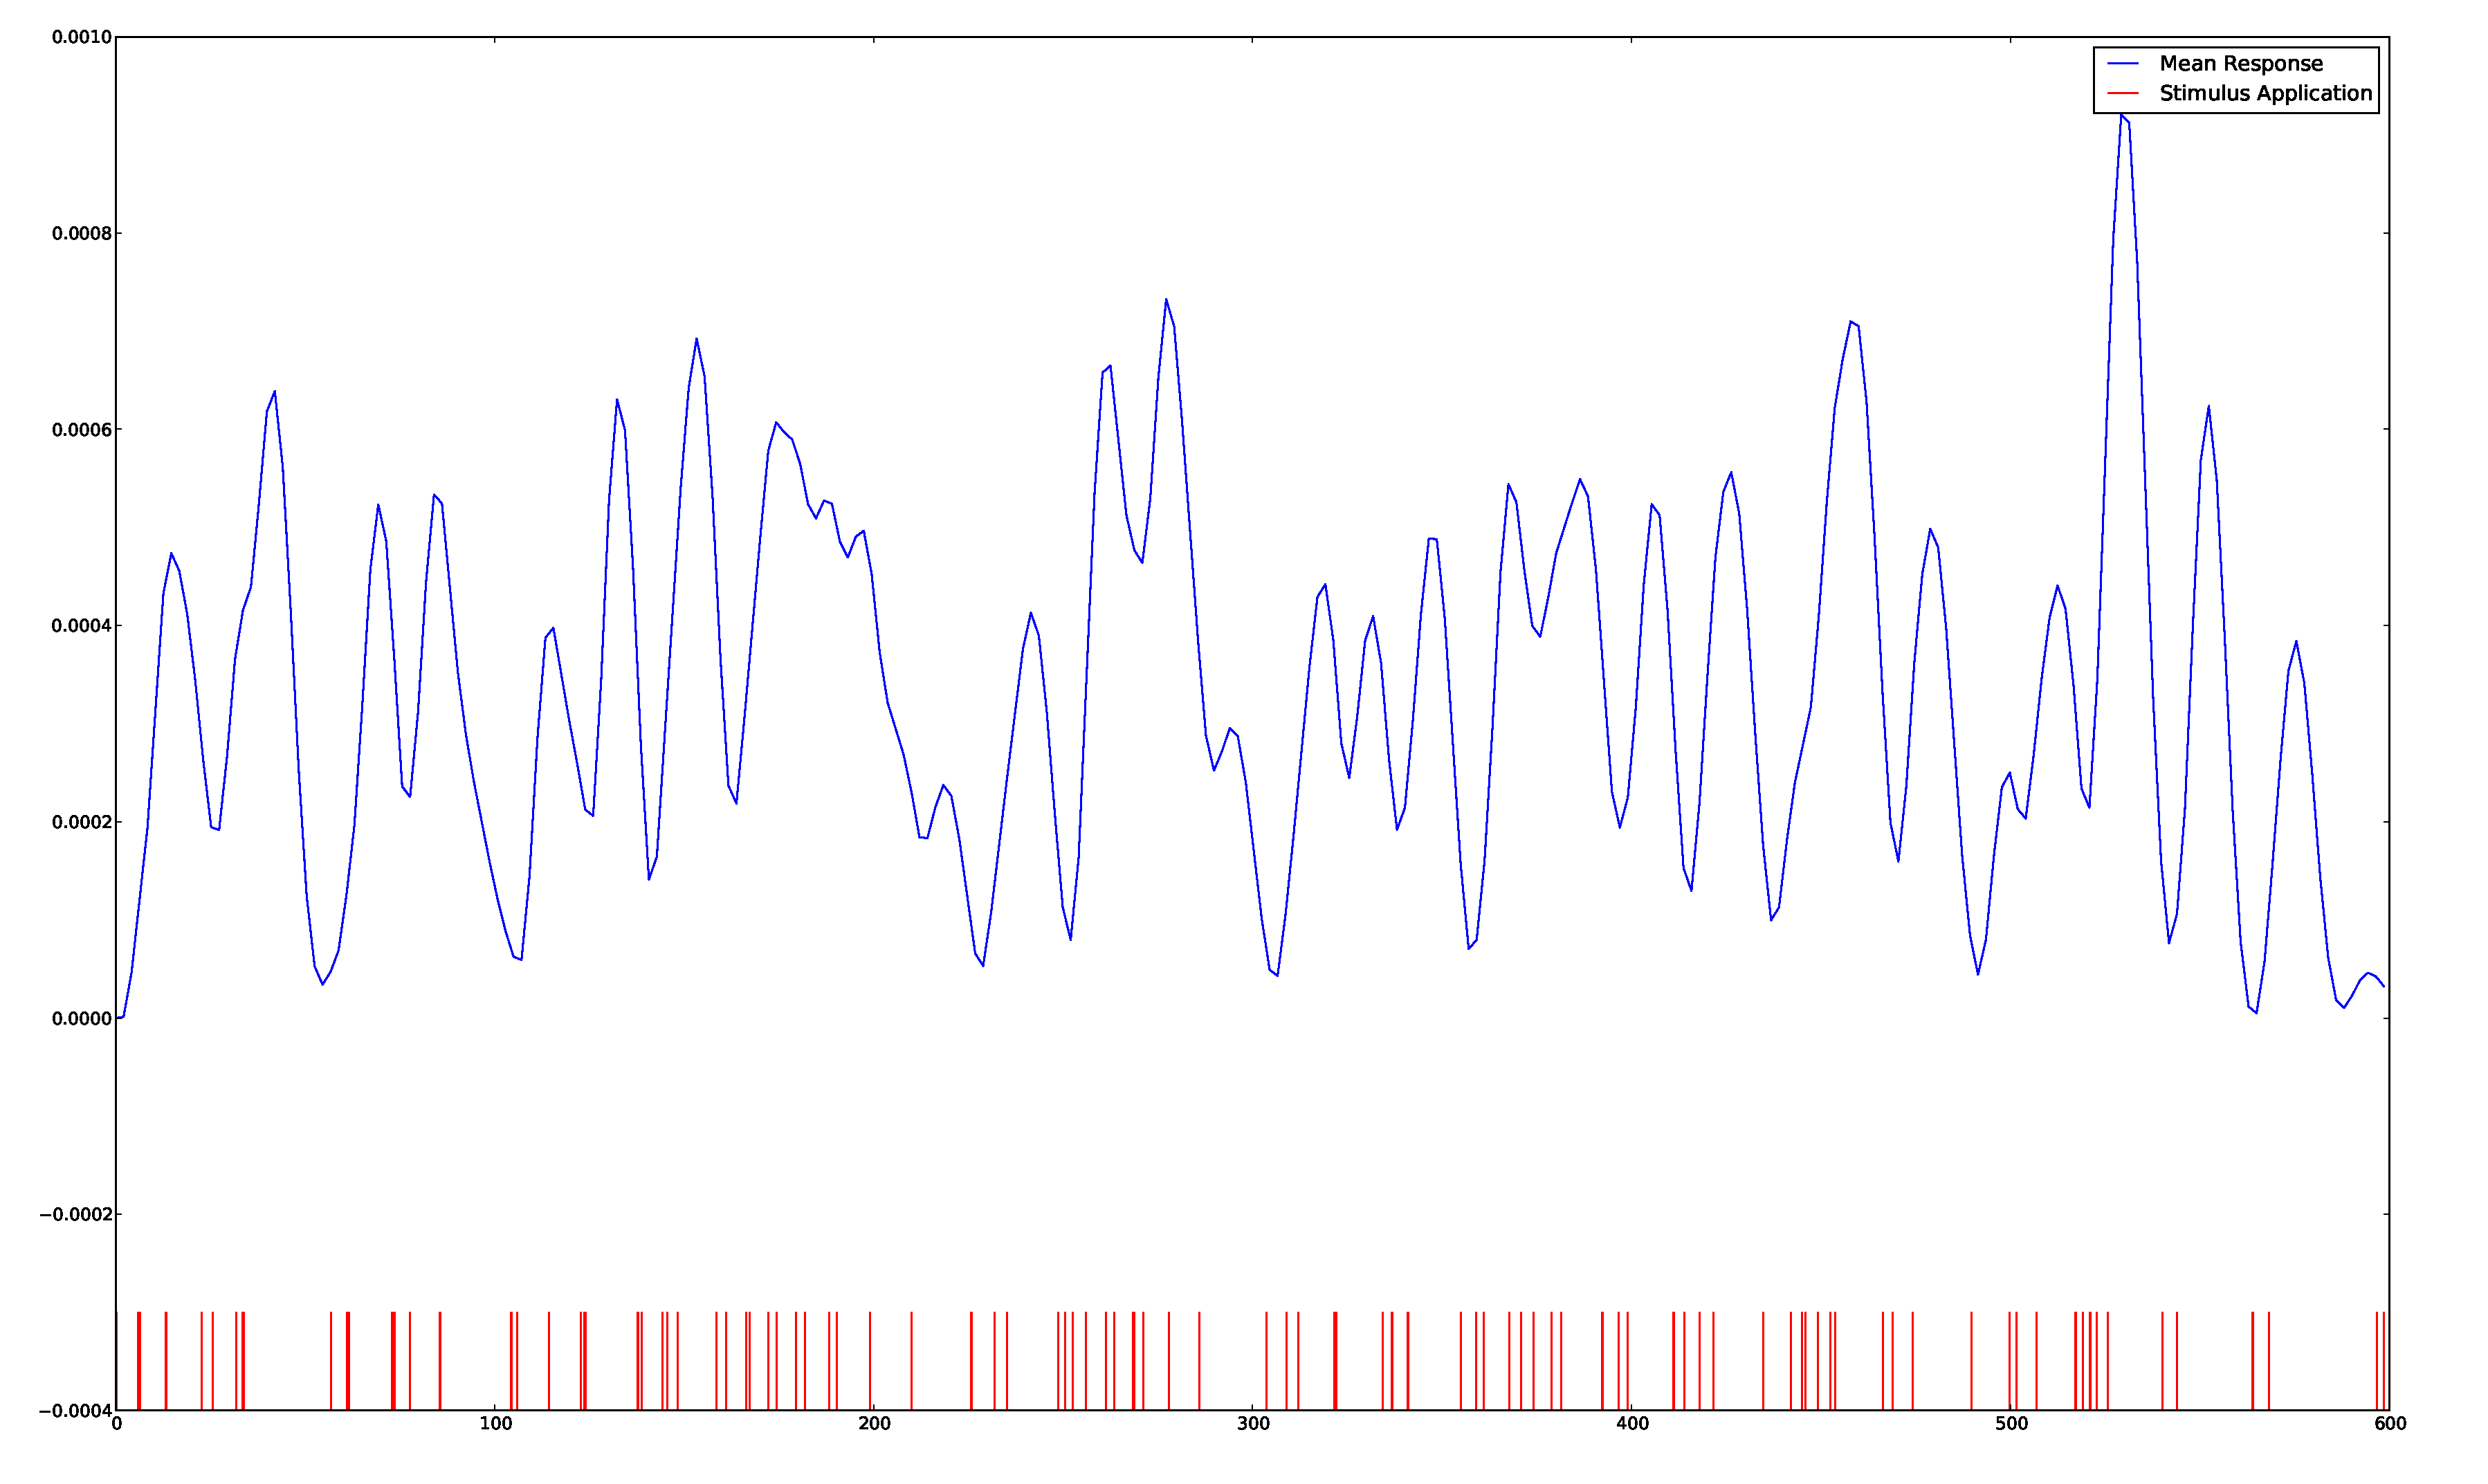
\includegraphics[trim=6cm 3cm 6cm 3cm,width=16cm]{images/mean_response_johnston}
\caption{Response to $.1s$ impulses with the mean parameters from \cite{Johnston2008}}
\end{figure}

Its likely that these differences are due to some difference in preprocessing,
although in \cite{Deneux2006} the signals were found to be peaking around
$1\%$, unlike \cite{Friston2000} which shows signals peaking at up to
$3\%$ or $4\%$. In my own tests, it seemed necessary for $\epsilon$ to
reach well over $1.5$ and $V_0$ to reach more than $.4$ to reach these
peaks; of course other methods may be equally able. 
Therefore, to account for these discrepancies, somewhat broader
distributions are used than the numbers used in \cite{Friston2000}
(which are widely used, \cite{Hu2009}). The 
priors used in the particle filter may be found in \autoref{tab:Prior}.

\begin{table}[t]
\centering
\begin{tabular}{|c || c | c | c |}
\hline 
Parameter & Distribution & $\mu$ & $\sigma$ \\
\hline
$\tau_0$ & Gamma & .98 & .25 \\
$\alpha$ & Gamma & .33 & .045\\
$E_0$    & Gamma & .34 & .03  \\
$V_0$    & Gamma & .04 & .03 \\
$\tau_s$ & Gamma & 1.54  & .25\\
$\tau_f$ & Gamma & 2.46  & .25\\
$\epsilon$ & Gamma & .7  & .6 \\
\hline
\end{tabular}
\caption{Prior distributions used in the particle filter.}
\label{tab:Prior} 
\end{table}

Note that although the mean remains the same for all the 
parameters other than $\epsilon$, the standard deviation is set
much higher to account for the disagreement between studies
(\autoref{tab:Params}). 
Because all the parameters are taken to be strictly positive, and the
standard deviations are approaching the mean, I used a gamma distribution.
This prevents the Gaussian from placing parameters in the nonsensical 
territory of negative activation, or negative time constants.

Another aspect of the prior is using enough particles to get a 
sufficiently dense approximation of the prior. For 7 dimensions,
getting a dense prior is difficult. Insufficiently
dense particles will result in inconsistent results. Of course the
processing time will scale up directly with the number of particles.
A dense initial estimate is important so that some particles land
near the solution; but as the variance decreases the number of 
particles needed decreases as well. Thus, as a heuristic, initially
the number of particles was set to 16,000, but after resampling,
the number of particles was dropped to 1,000. Typically during the 
first few measurements the variance dropped precipitously because
most particles were far from a solution.  The particles that are left are in a
much more compact location, allowing them to be estimated with 
significantly fewer particles. These numbers aren't set in stone,
and depending on the complexity of the system or desired accuracy
they could be changed; however, they seem to be the minimum that
will give consistent results.

\section{Resampling}
\label{sec:Resampling}
The algorithm for resampling is described in \autoref{sec:Particle Filter Resampling}.
When regularizing, the Gaussian kernel is convenient,
because it is simple to sample from and long tailed.
As discussed in \autoref{sec:Particle Filter Resampling},
as long as resampling is kept as a last resort, some over-smoothing
doesn't impair convergence. Therefore, for this work I chose a Gaussian kernel of
bandwidth equal to the original distribution's covariance. Obviously this will
apply a rather large amount of smoothing to the distribution; however, on average
resampling is only applied every 20 to 30 measurements, and because randomization
is being applied to model updates this gives the filter some mobility. 

Re-sampling is a not strictly necessary, but increases the effectiveness
of the particle filter by adjusting the support to emphasize areas
of higher probability. Re-sampling is slow because it requires re-drawing
all the particles. It also closes off avenues of investigation, and is
designed to over-smooth to prevent overly thinning the support. For all these
reasons, resampling was only performed when the $N_{eff}$ dropped below
50 (for 1000 particles).  As a measure against sharp drops in the $N_{eff}$ 
caused by a large spike in error, resampling was only performed when 
two consecutive low ($<50$) $N_{eff}$'s were found. 

\section{Choosing $P(y_k | x_k)$}
\label{sec:Methods Weighting Function}
The choice of $P(y_k | x_k)$ is the second most important design decision, behind 
the prior. While the conventional choice for an unknown distribution is the 
Gaussian, there are reasons why it may not be the best in this case.  
As noted in \autoref{sec:Introduction Noise}, the noise is not strictly Gaussian,
nor is it strictly Wiener. As with any unknown noise however, it is necessary 
to make some assumption. If the weighting function ($P(y_k | x_k)$) exactly
matches the measurement error, then the ideal particle filter will result.
Particles with $x_k$'s that repeatedly estimate $y_k$ with large residual 
will quickly have weights near 0. Thus, a weighting function that
exactly matches $P(Y(t) | X(t))$ will easily, and correctly throw out incorrect
particles.  The cost of choosing an overly broad distribution for this
function is slow convergence.  On the other hand, an overly thin 
distribution will lead to particle deprivation (all particles
being zero-weighted).  I tested several weighting
functions: in addition to the Gaussian I also tested the Laplace and Cauchy
distributions, both of which have much wider tales than the Gaussian. 
Wider tailed distributions don't down-weight
particles as fast; and converge more slowly (and perhaps more accurately). 
The Laplace distribution also has the
benefit of a non-zero slope at the origin; which means that even
it will distinguish between particles even near the origin.

After trial and error, for this work I chose a zero-mean Gaussian with standard deviation 
of $.005$. While I made some attempts to automatically set the standard 
deviation, results were often unpredictable. If the weight function and scale aren't
fixed across voxels, very noisy time series with no actual signal 
converged to nonsensical results. 
In the future, it may be possible to set the standard deviation by
taking a small sample from resting data and using the sample standard deviation.
Since this is the first attempt at using particle filters for modeling the 
BOLD model, in this work I set the standard deviation manually at $.005$,
because it gave the best consistency. 

\subsection{Runtime}
The run-time for a single voxel depends on the several factors. First, the
overall length of the signal being analyzed. For 1000 measurements it takes
about 6 minutes. On the other hand, in real circumstances the
length is only around 150 measurements and takes around 40 seconds (for 1000 
particles, 1500 integration points and a Quad Core CPU). The size of 
local linearization steps are also crucial although going above .001 seconds
per step is not recommended. In most cases millisecond resolution
is fine; however, when generating simulated data I found that at times it was
still not enough every once. This is problematic in the actual particle
filter since, given the large number of simultaneous integrations taking 
place, its probable that a few particles will fail and be unfairly thrown away.
To prevent such events, 1500 integration points per second were used throughout
the tests. 

Another crucial factor for run time is how long before the first re-sampling 
occurs. Because the prior is represented initially with significantly more
particles, if for some reason the effective
number of particles stays high, resampling could take a long time to occur.
For this reason, rather than allowing the particle filter to continue on 
with this large number of particles, after 20 seconds have passed the
algorithm forces resampling. The choice of 20 seconds is 
arbitrary, but at the very least it gives a more optimized version of the
prior. 


\chapter{Results}

\section{Simulation}
I performed two types of simulations. First, I simulated a single BOLD time-series based
on a randomly selected set of model parameters. Second I used a modified version of the
FSL tool possum to generate a noisy FMRI image. 

\subsection{Single Timeseries}
This process was relatively straight forward,
given the state-space equations for the BOLD signal. After a "true" signal was generated,
I then added a identically and independently distributed (I.I.D.) Gaussian noise and a Wiener
process with Gaussian I.I.D. steps. Finally a carrier level was added, since BOLD is typically
measured as a \% difference from the
base level. Adding a carrier level meant that the exact same algorithm which was used for 
real data could be used for the simulated data. 

Once this noisy simulated time series was generated, the particle filter algorithm
 was run on this single timeseries image. In order to find the best setting for the
particle filter I ran quite a few tests. Here I will include two sets of tests 
to determine the power of the particle filter in modeling. The first test is
low noise $\{\sigma_y = .001, \sigma_x = .0005\}$, while the second set of
tests had noise of $ \{\sigma_y = .01, \sigma_x = .005\} $, where $\sigma_y$ is the
measurement noise, and $\sigma_x$ is the wiener step size. Both signals used the
parameters ($\tau_0 = 1.45, \alpha = .3, E_0 = .47, V_0 = .044, \tau_s = 1.94, \tau_f = 1.99, \epsilon = 1.8$).
The particle filter used the parameters defined in \autoref{tab:Prior} (\autoref{sec:PriorDistrib}),
thus the particle filter was not centered over the correct values. 

\subsubsection{Low Noise Simulation}
For the low noise case, the ten realization are shown in \autoref{fig:LowNoiseRealization}.
\begin{figure}
\label{fig:LowNoiseRealization}
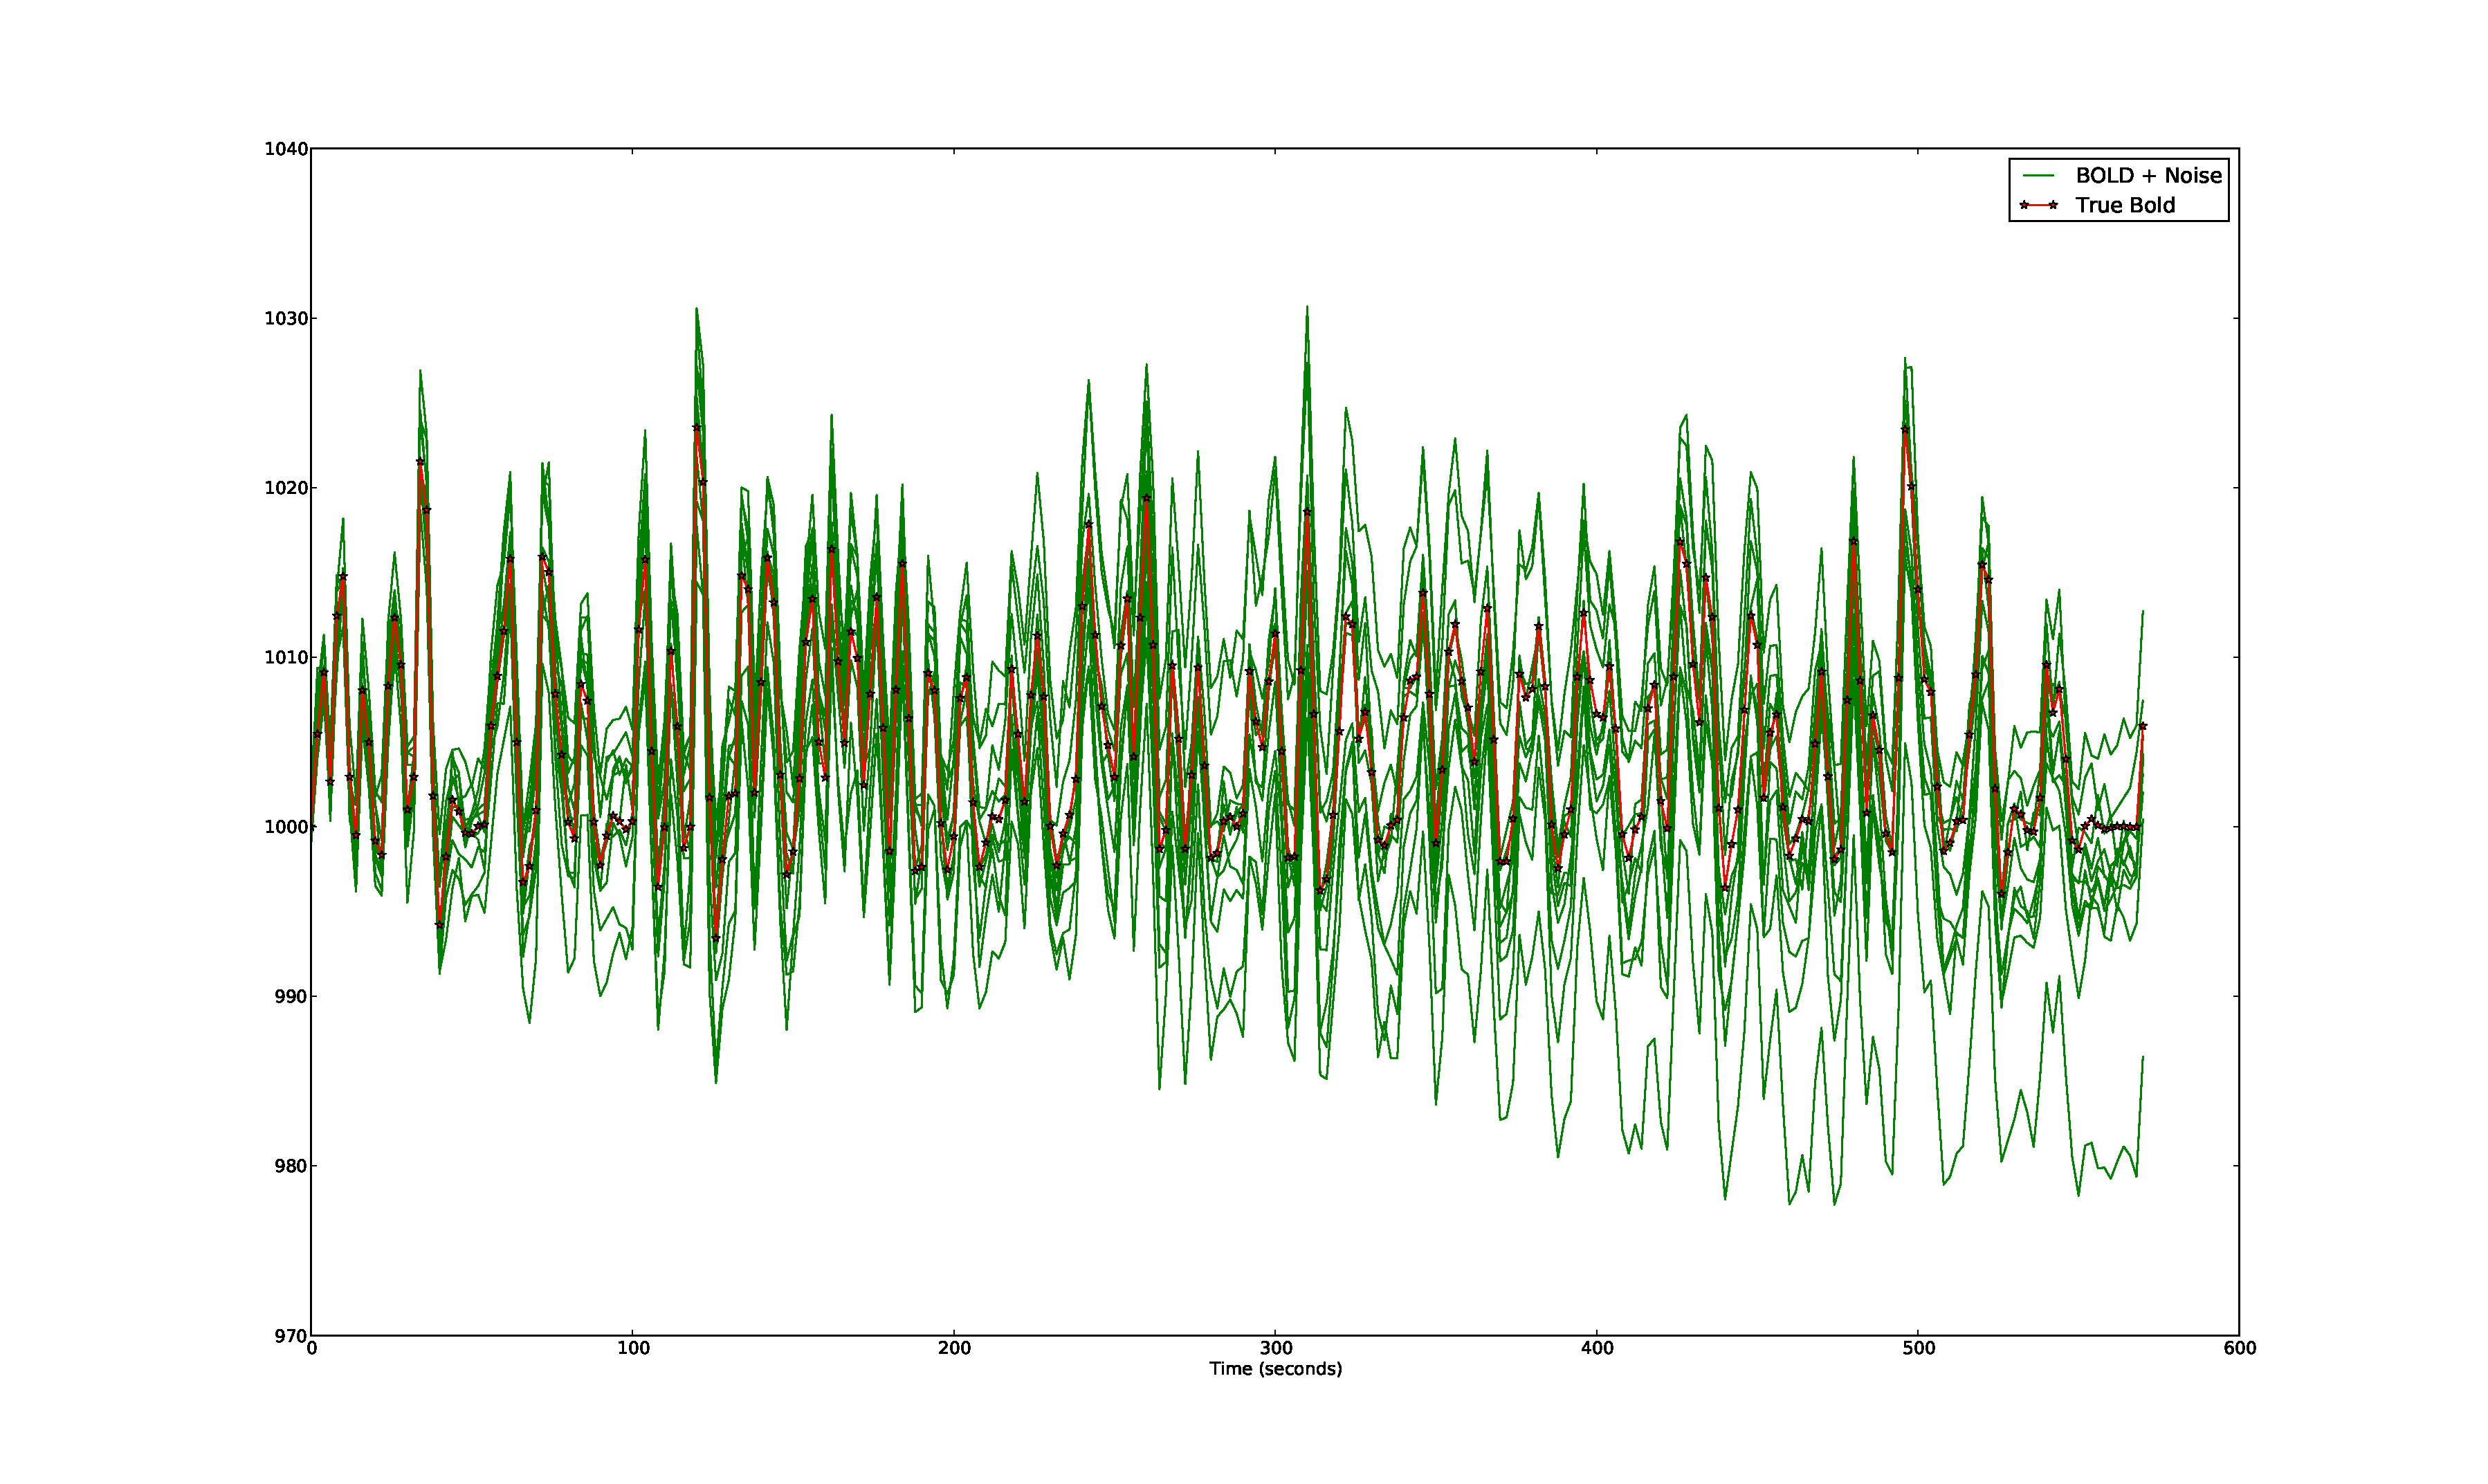
\includegraphics[trim=6cm 3cm 6cm 3cm,width=16cm]{images/realization_lownoise}
\caption{Test Signals with low noise compared to the clean signal}
\end{figure}

The resulting fits compared to the \emph{true} BOLD signal are shown in \autoref{fig:FitComparisonLowNoise}.
The fits are good, but the noise is relatively low. The preprocessed signal compared
to the true BOLD signal is shown in \autoref{fig:PreprocessedLowNoise}.

\begin{figure}
\label{fig:PreprocessedLowNoise}
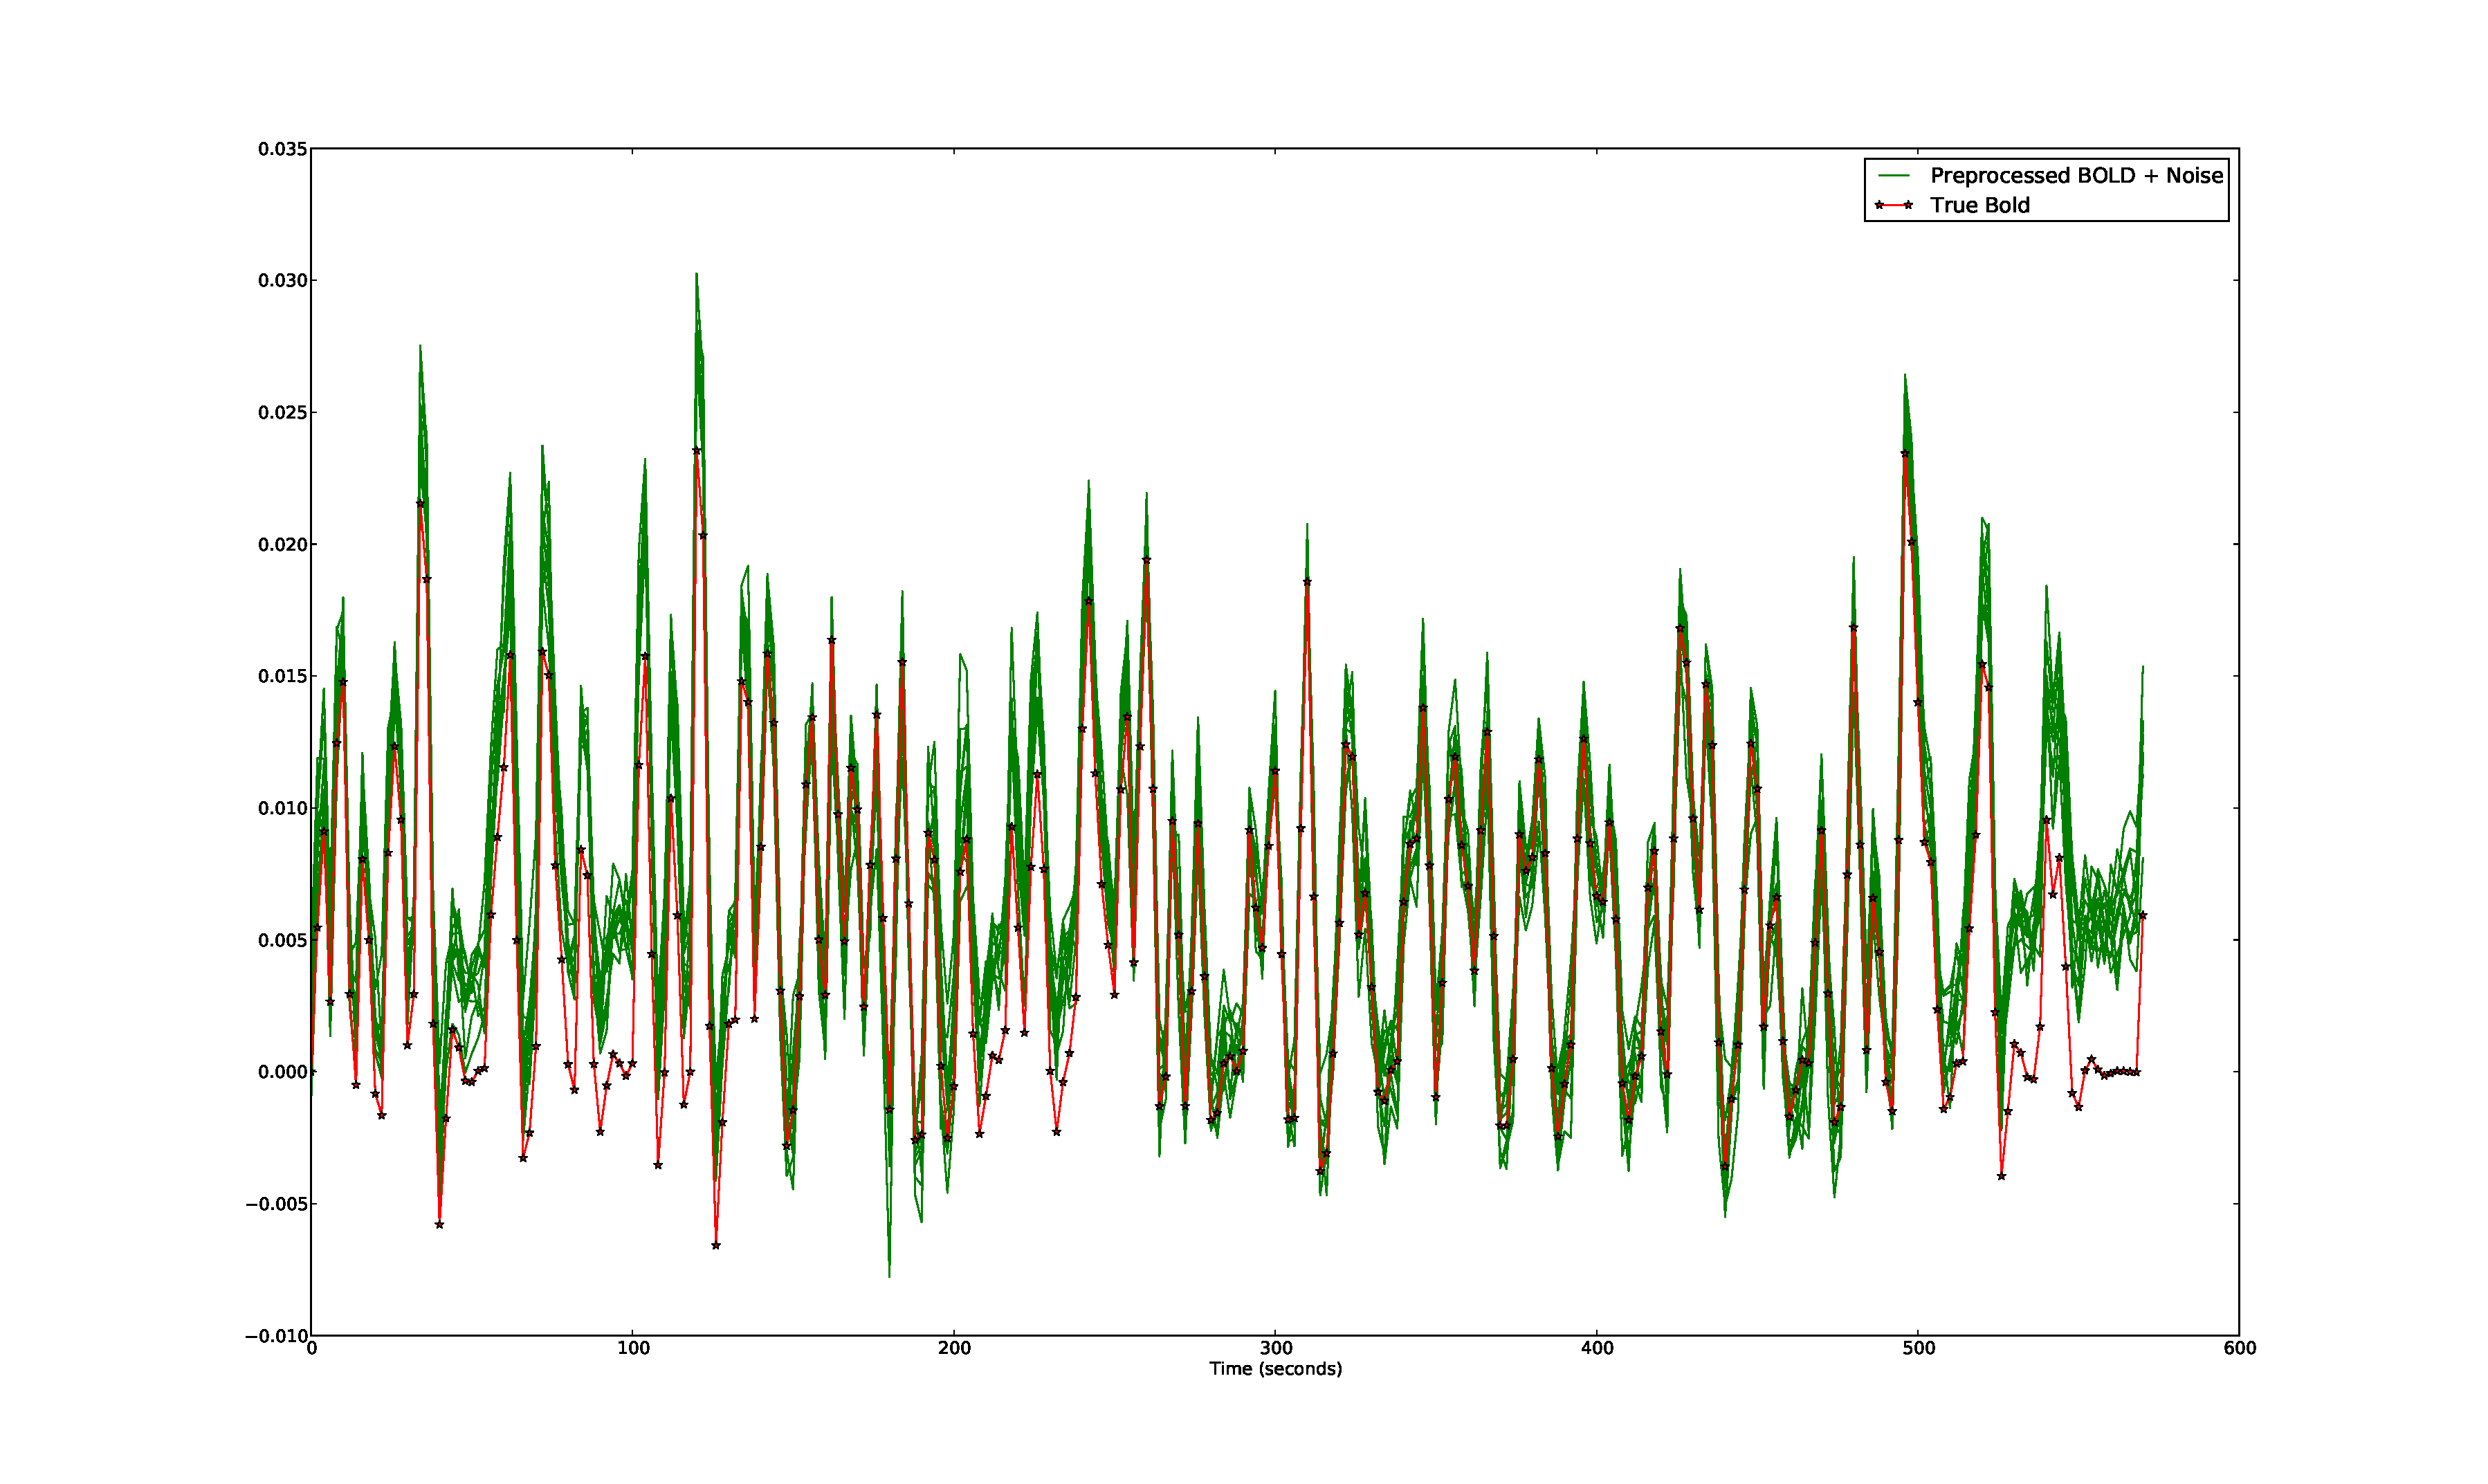
\includegraphics[trim=6cm 3cm 6cm 3cm,width=16cm]{images/preprocessed_lownoise}
\caption{A comparison of the preprocessed signals for the low noise case.}
\end{figure}

The preprocessing consists of several steps, which are discussed in detail in \autoref{sec:Preprocessing}.
Obviously the spline struggles a little bit at the end, as the graph shows, although 
overall the fit is pretty well. Finally, the set of fits to the preprocessed data, and in 
essence to the "true" BOLD signal is shown in \autoref{fig:FitComparisonLowNoise}.

\begin{figure}
\label{fig:FitComparisonLowNoise}
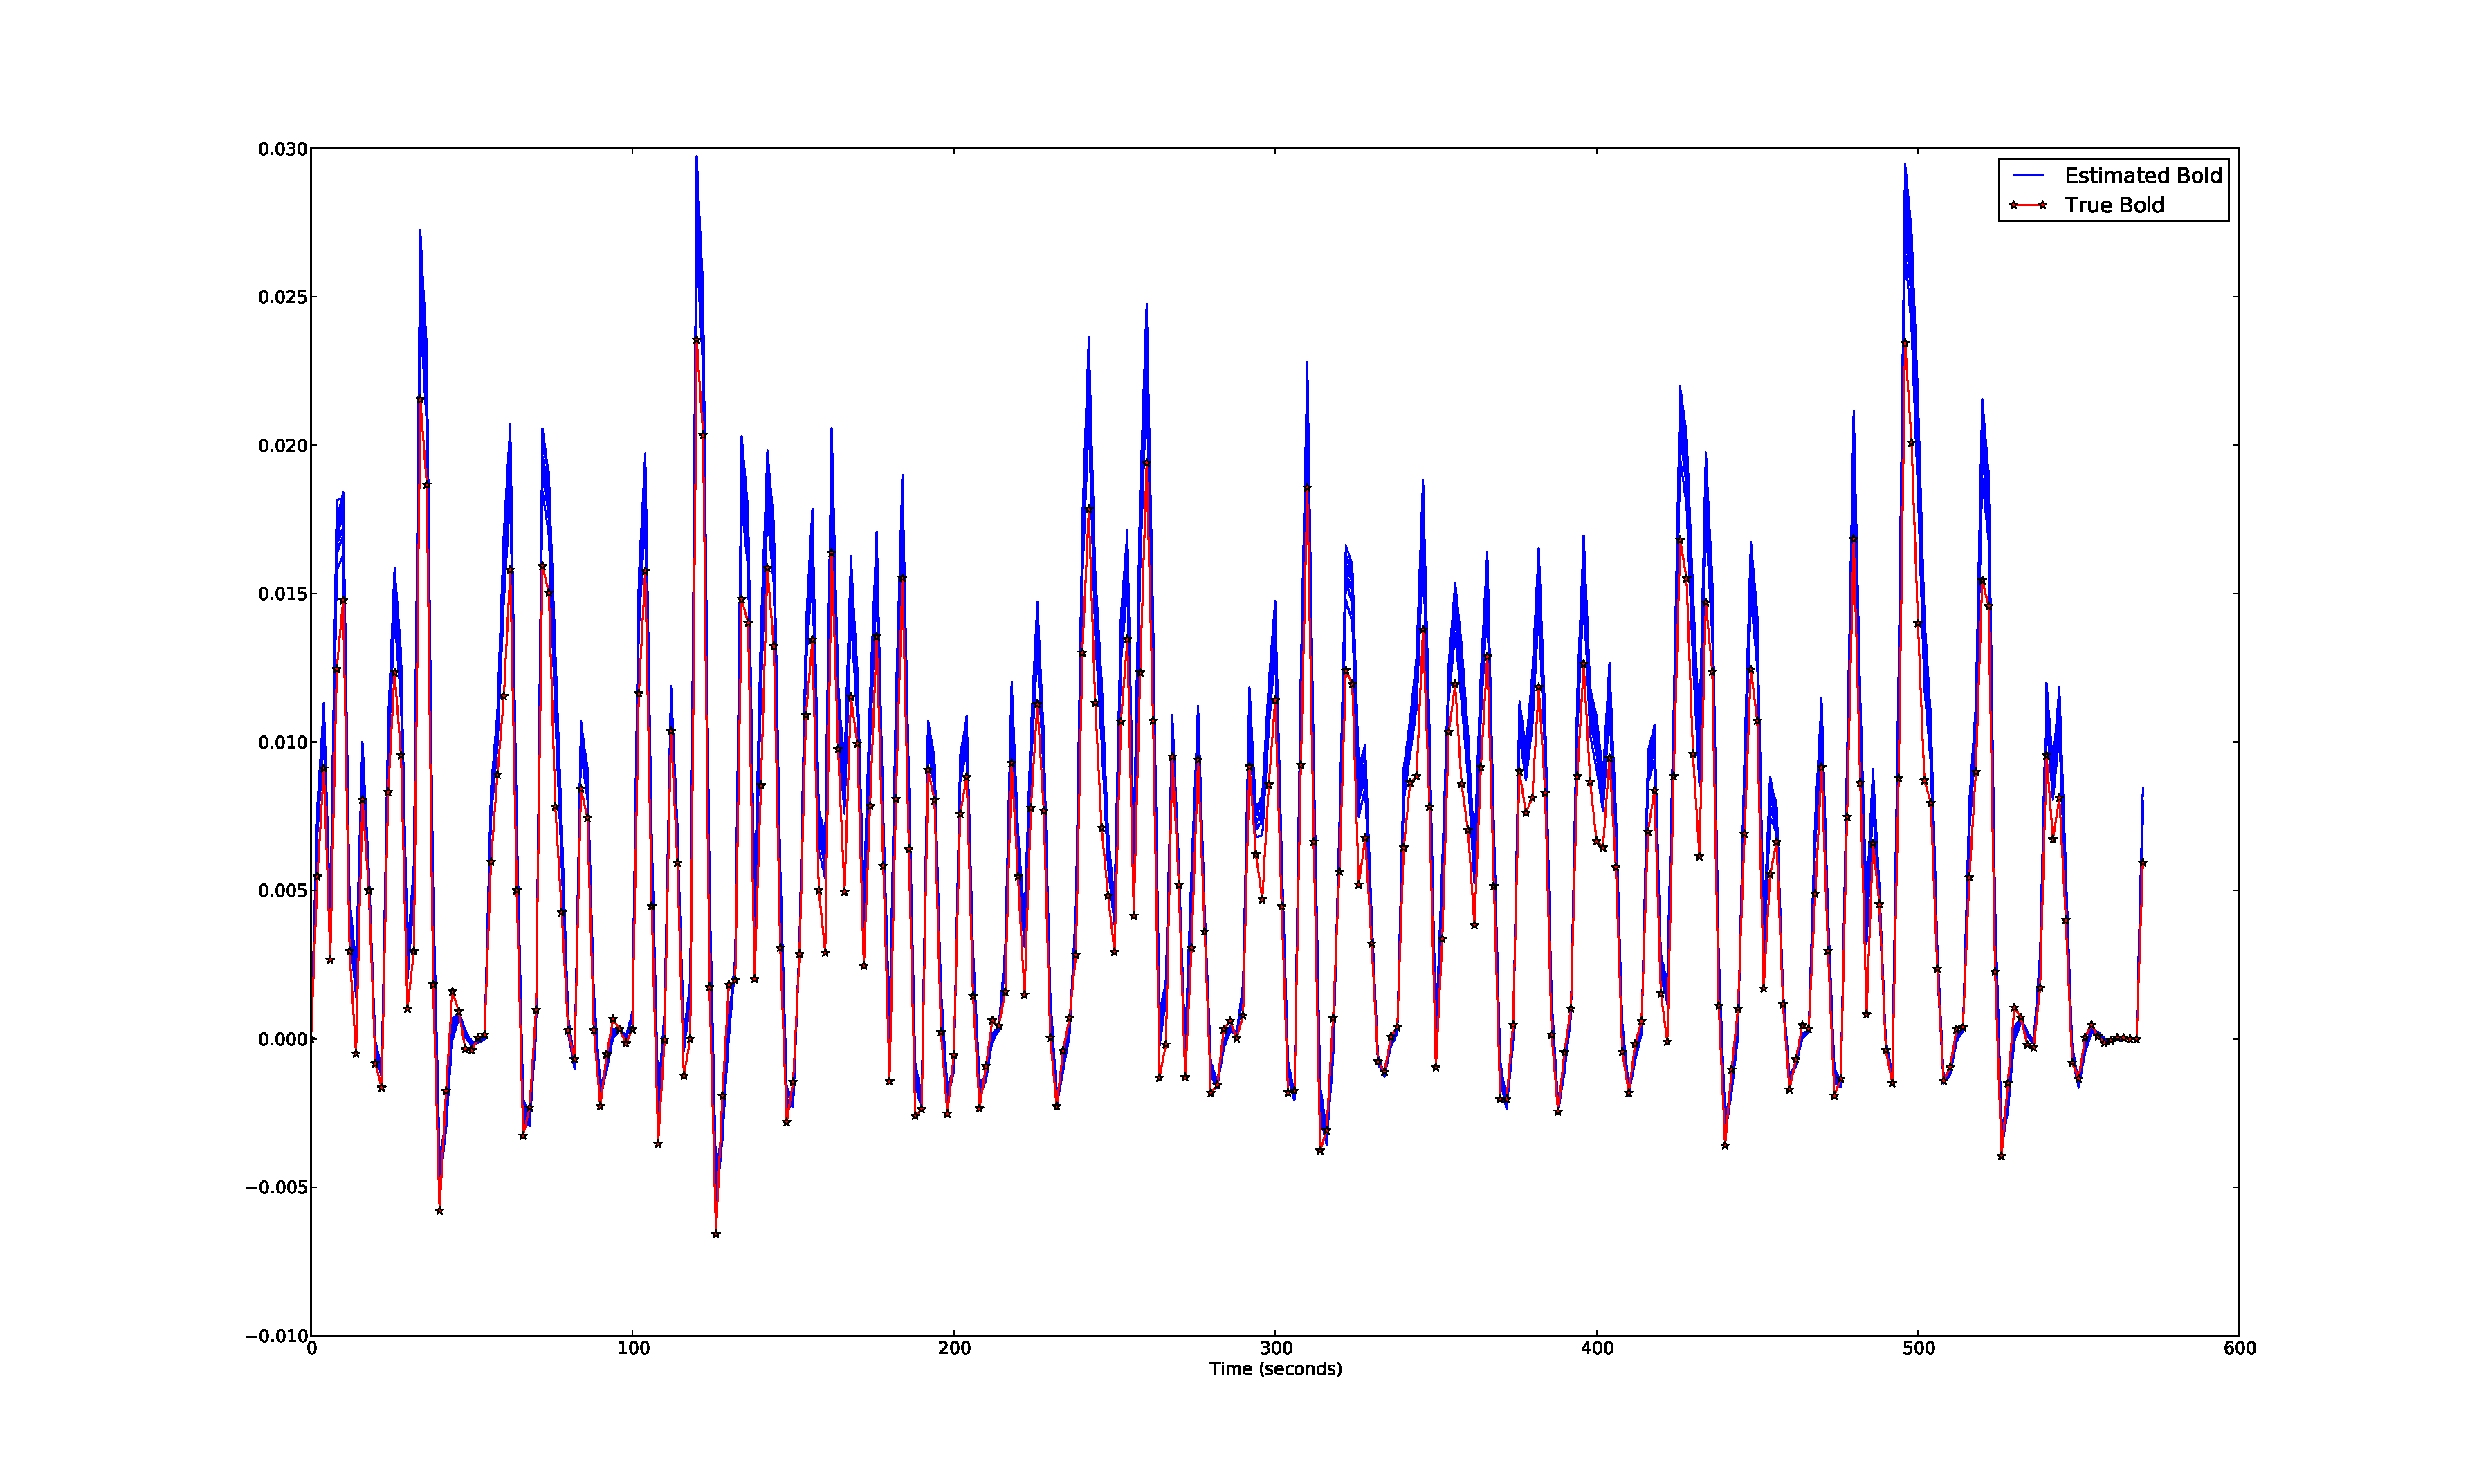
\includegraphics[trim=6cm 3cm 6cm 3cm,width=16cm]{images/comparison_lownoise}
\caption{A comparison of the fitted signals for the low noise case.}
\end{figure}

It becomes clear now the reason for the term particle filter. In several locations the output
of the particle filter looks like a filtered version of the input. For instance toward the
end, the estimates stay flat in spite of the preprocessed data drifting off a bit. By
this point, the algorithm had converged sufficiently to know that that wasn't possible.
A similar circumstance occurs at 100 seconds in. In general the fits are good, although because
of the slightly higher signal levels in the preprocessed signals, the fits tend to overestimate
the peak a bit. The final parameter sets are shown in \autoref{tab:LowNoiseParams}
\begin{table}[t]
\centering
\begin{tabular}{|c | c | c | c | c | c | c | c | c | c |}
\hline 
$\tau_0$ & $\alpha$ & $E_0$    & $V_0$    & $\tau_s$ & $\tau_f$ & $\epsilon$  & $ \sum \tau $ & $\sqrt{MSE}$ (Res.) &$\sqrt{MSE}$\\
\hline 
\rowcolor[gray]{.8}
1.45 & .3 & .47 & .044 & 1.94 & 1.99 & 1.8  & 5.38 &  & \\
\hline 
\hline 
1.22214 & 0.3449 & 0.33462 & 0.07138 & 1.60446 & 2.27529 & 1.59454 & 5.10189  &  0.00321067  & 0.00987647  \\
1.37493 & 0.33183 & 0.36296 & 0.07327 & 1.64076 & 2.10299 & 1.57627 & 5.11867 &  0.00305475  & 0.00993227  \\
1.16604 & 0.32205 & 0.34057 & 0.08217 & 1.64768 & 2.35351 & 1.24515 & 5.16722 &  0.00328932  & 0.00967961  \\
1.23176 & 0.32707 & 0.34028 & 0.07961 & 1.62698 & 2.18519 & 1.30326 & 5.04394 &  0.00284719  & 0.00912005  \\
1.1832 & 0.31787 & 0.34718 & 0.0821 & 1.54961 & 2.29115 & 1.27817 & 5.02396   &  0.00300634  & 0.00971258  \\
1.1424 & 0.33395 & 0.34725 & 0.07366 & 1.62208 & 2.29084 & 1.4025 & 5.05531   &  0.00283287  & 0.00948483  \\
1.30041 & 0.3596 & 0.35643 & 0.07679 & 1.56406 & 2.13234 & 1.60338 & 4.99681  &  0.00302802  & 0.01021885  \\
1.24008 & 0.34601 & 0.33978 & 0.08903 & 1.64989 & 2.23655 & 1.29004 & 5.12651 &  0.00304378  & 0.01007964  \\
1.1709 & 0.32739 & 0.34644 & 0.08255 & 1.53734 & 2.28262 & 1.37828 & 4.99087  &  0.00334488  & 0.01032886  \\
1.18967 & 0.34344 & 0.33554 & 0.07976 & 1.53582 & 2.30746 & 1.42774 & 5.03295 &  0.00317542  & 0.01001503  \\
1.184 & 0.34053 & 0.35017 & 0.08917 & 1.61025 & 2.27926 & 1.16448 & 5.07352   &  0.00288855  & 0.00950536  \\
\hline                                                                           
1.21868 & 0.33588 & 0.34557 & 0.07995 & 1.59899 & 2.24884 & 1.38762 & 5.06651 & 0.00306562     & 0.00981396 \\
\hline 
\end{tabular}
\caption{Estimated Parameters on 10 different runs with low noise. First row is the true parameters,
last is mean over the 10 runs. The $\sqrt{MSE}$ (Res.) is the square root of the mean square of the
residuals. Essentially this is the is the MSE between the estimated signal and the noisy signal which 
was available to the particle filter. Square root of MSE is the actual \emph{error}, with the true signal,
which of course was not available to the particle filter.}
\label{tab:LowNoiseResults} 
\end{table}

There are a few things worth noting here. First the time constants vary greatly across
runs with different noise realizations, yet the sum of the individual time constants
, $\tau_f$, $\tau_s$ and $\tau_0$ seem to be more consistent. In general the 
time constants are falling short of the true time constant. This could be a limitation
based on the prior distribution (which notably has mean values below the values used
in the simulation) or it could be caused by the delayed benefit of having a 
correct time constant. Even if one particle has a better time constant than another, if
the difference isn't severe, by the time this makes a difference in the weight, the 
particle with the better $\tau$ will have been weighted based on other parameters several
times. Another interesting result in the huge variation in the levels of $V_0$. In general,
with this admittedly small amount of noise, it would appear that the relation between a set
of parameters/stimuli with the output is not injective. In other words, it would appear
that a timeseries is not unique to a set of parameters. This is good justification that 
simultaneous blood volume or tagged flow calculations with the conventional FMRI 
could definitely benefit the model. 

\begin{table}[t]
\centering
\begin{tabular}{|c | c  c  c  c  c  c  c |}
\hline 
  & $\tau_0$ & $\alpha$ & $E_0$    & $V_0$    & $\tau_s$ & $\tau_f$ & $\epsilon$ \\
\hline 
\rowcolor[gray]{.8} $\tau_0$ &   0.0189481 & -0.0014269 & -0.0011267 & -1.13e-05 & -0.0025616 & -0.0189559 & 0.0070405 \\
$\alpha$ &                       -0.0014269 & 0.0026716 & 9.93e-05 & -0.0002041 & -0.0008632 & -0.0016823 & 0.0071891 \\
\rowcolor[gray]{.8} $E_0$    &   -0.0011267 & 9.93e-05 & 0.0010701 & -0.0002277 & -0.0001177 & 0.0001013 & 0.0016972 \\
$V_0$    &                       -1.13e-05 & -0.0002041 & -0.0002277 & 0.0005401 & 4.3e-06 & 4.56e-05 & -0.0080494 \\
\rowcolor[gray]{.8} $\tau_s$ &   -0.0025616 & -0.0008632 & -0.0001177 & 4.3e-06 & 0.0128056 & 0.012878 & -0.005516 \\
$\tau_f$ &                       -0.0189559 & -0.0016823 & 0.0001013 & 4.56e-05 & 0.012878 & 0.0416927 & -0.0158182 \\
\rowcolor[gray]{.8} $\epsilon$&  0.0070405 & 0.0071891 & 0.0016972 & -0.0080494 & -0.005516 & -0.0158182 & 0.1567165 \\
\hline 
\end{tabular}
\caption{Typical Covariance matrix of the parameters at the end of a run.}
\label{tab:CovSim} 
\end{table}

\begin{figure}[H]
\subfigure[Converging histogram for $\tau_0$, $\alpha$, $E_0$, and $V_0$ of the first run, low noise simulation.]
{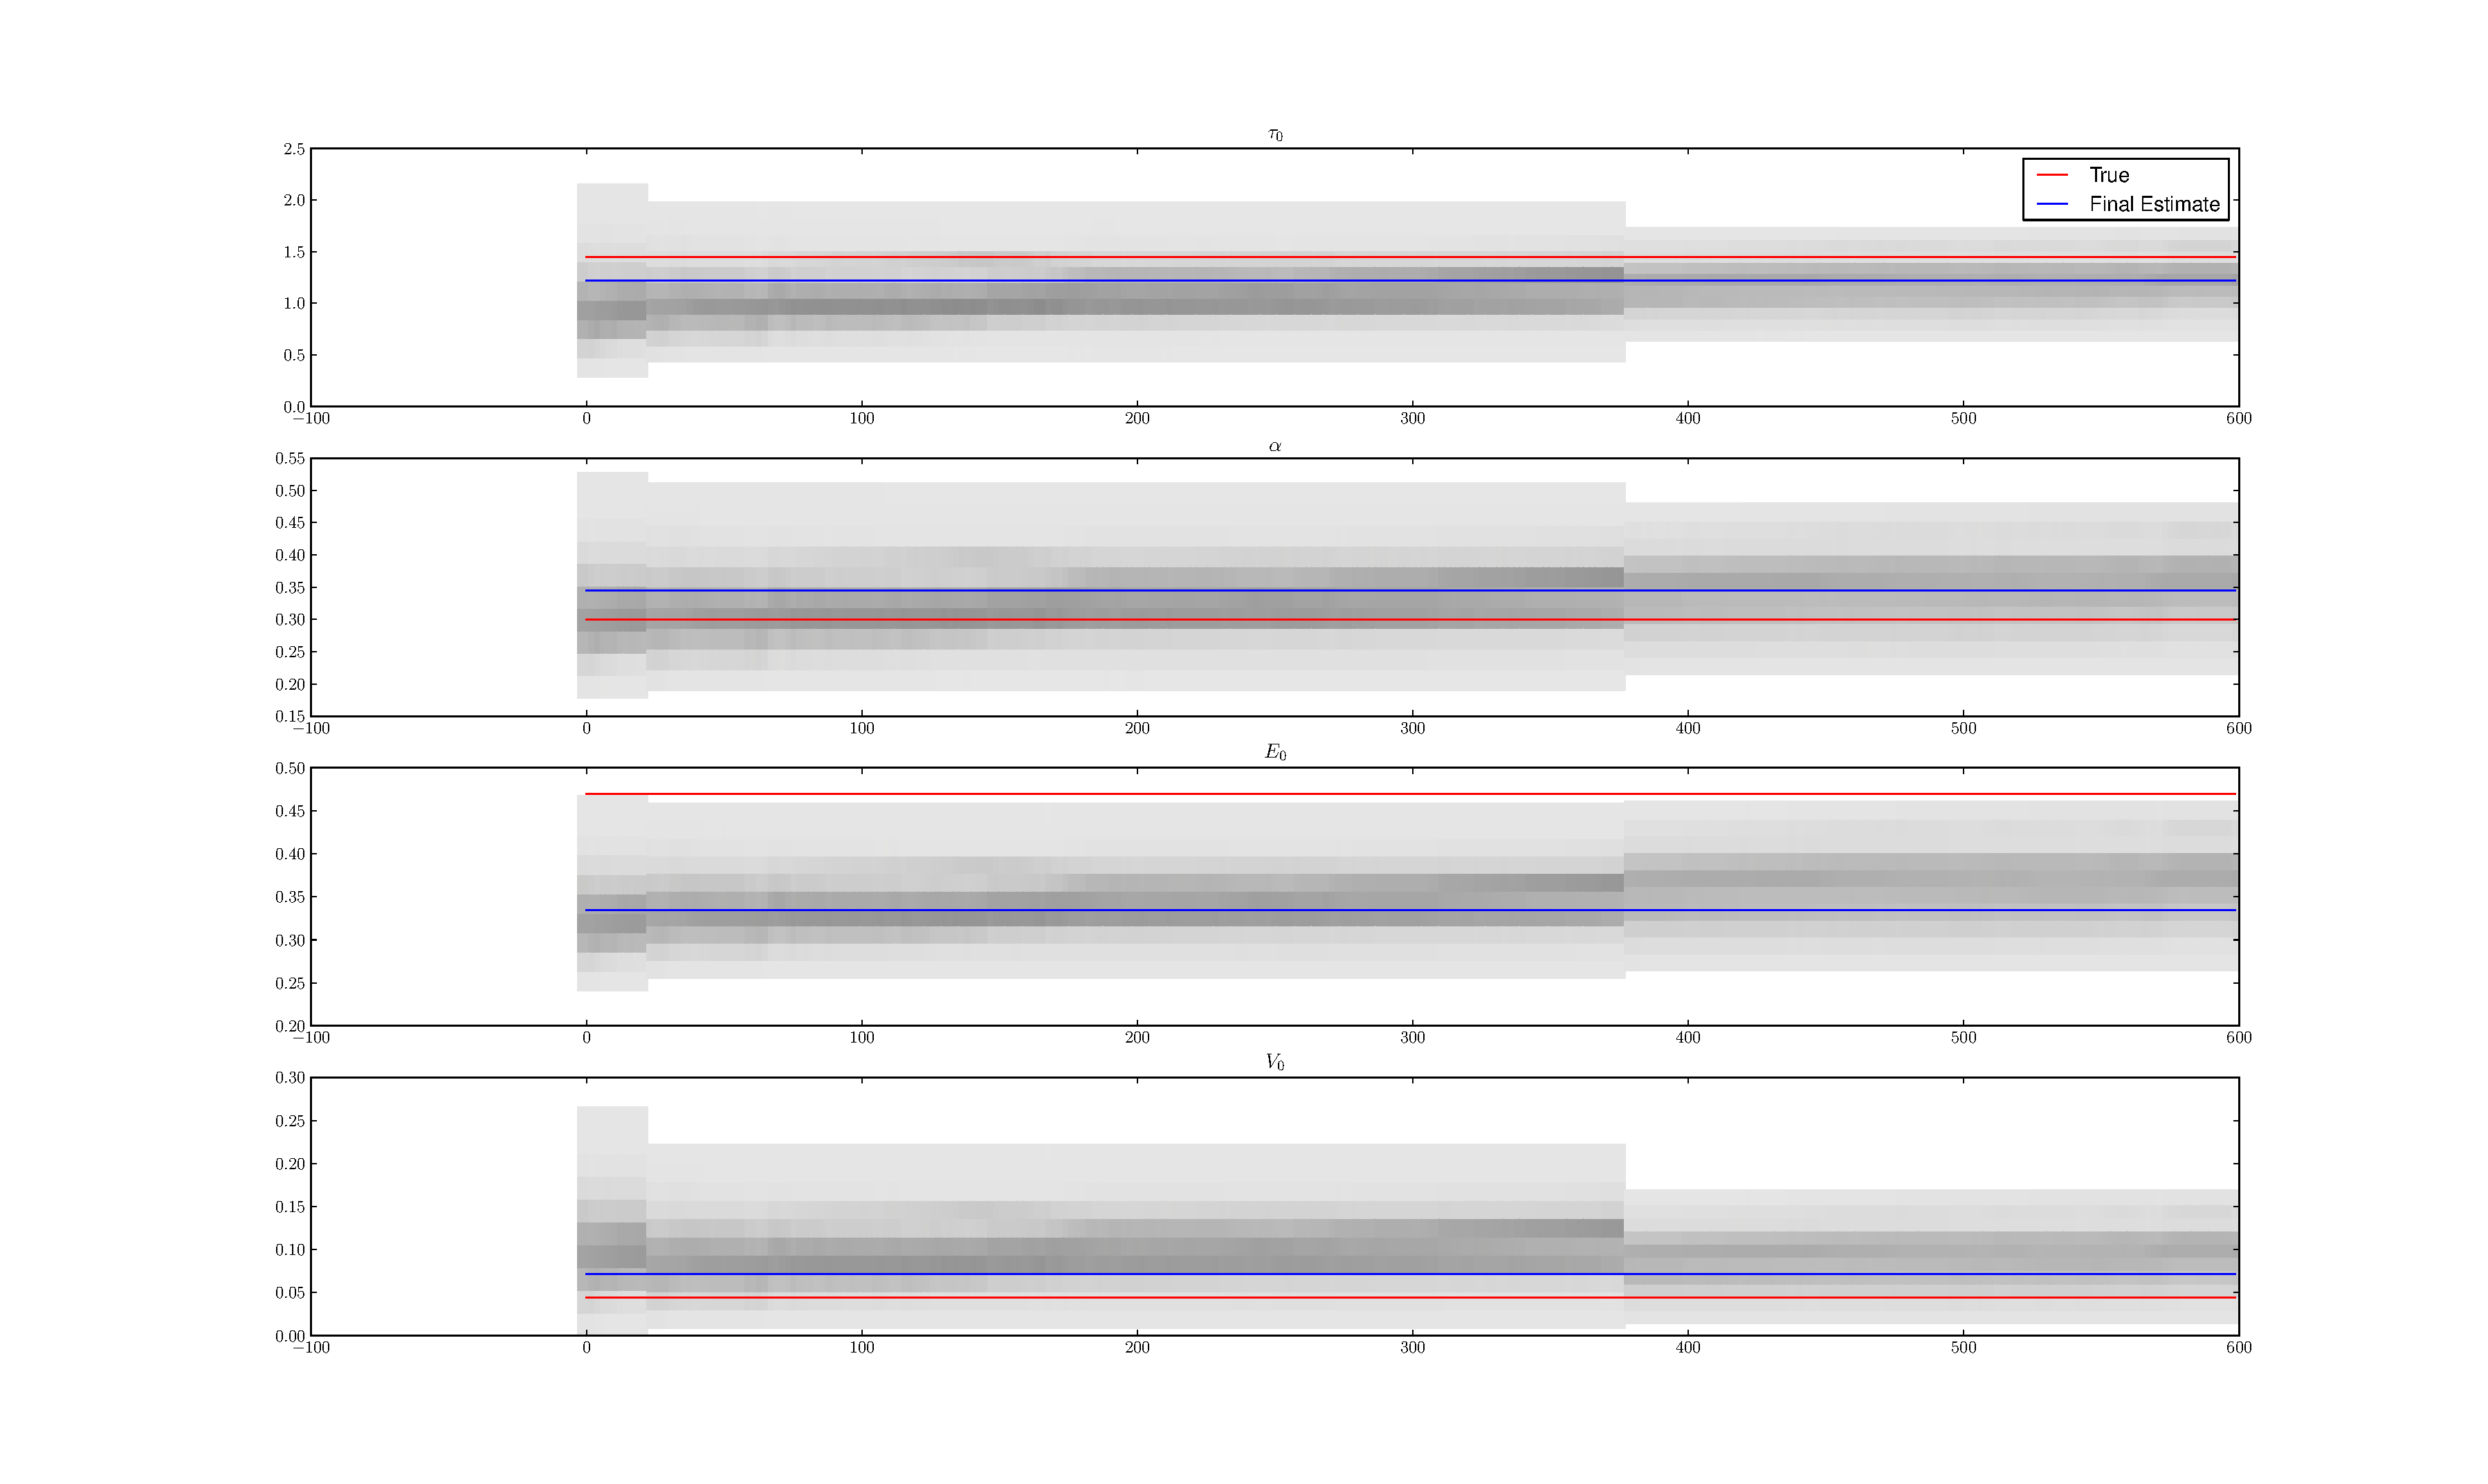
\includegraphics[trim=7cm 4cm 7cm 4cm, width=15cm]{images/converge_lownoise1}}\\

\subfigure[Converging histogram for $\tau_s$, $\tau_f$, $\epsilon$, and $V$ of the first run, low noise simulation.]
{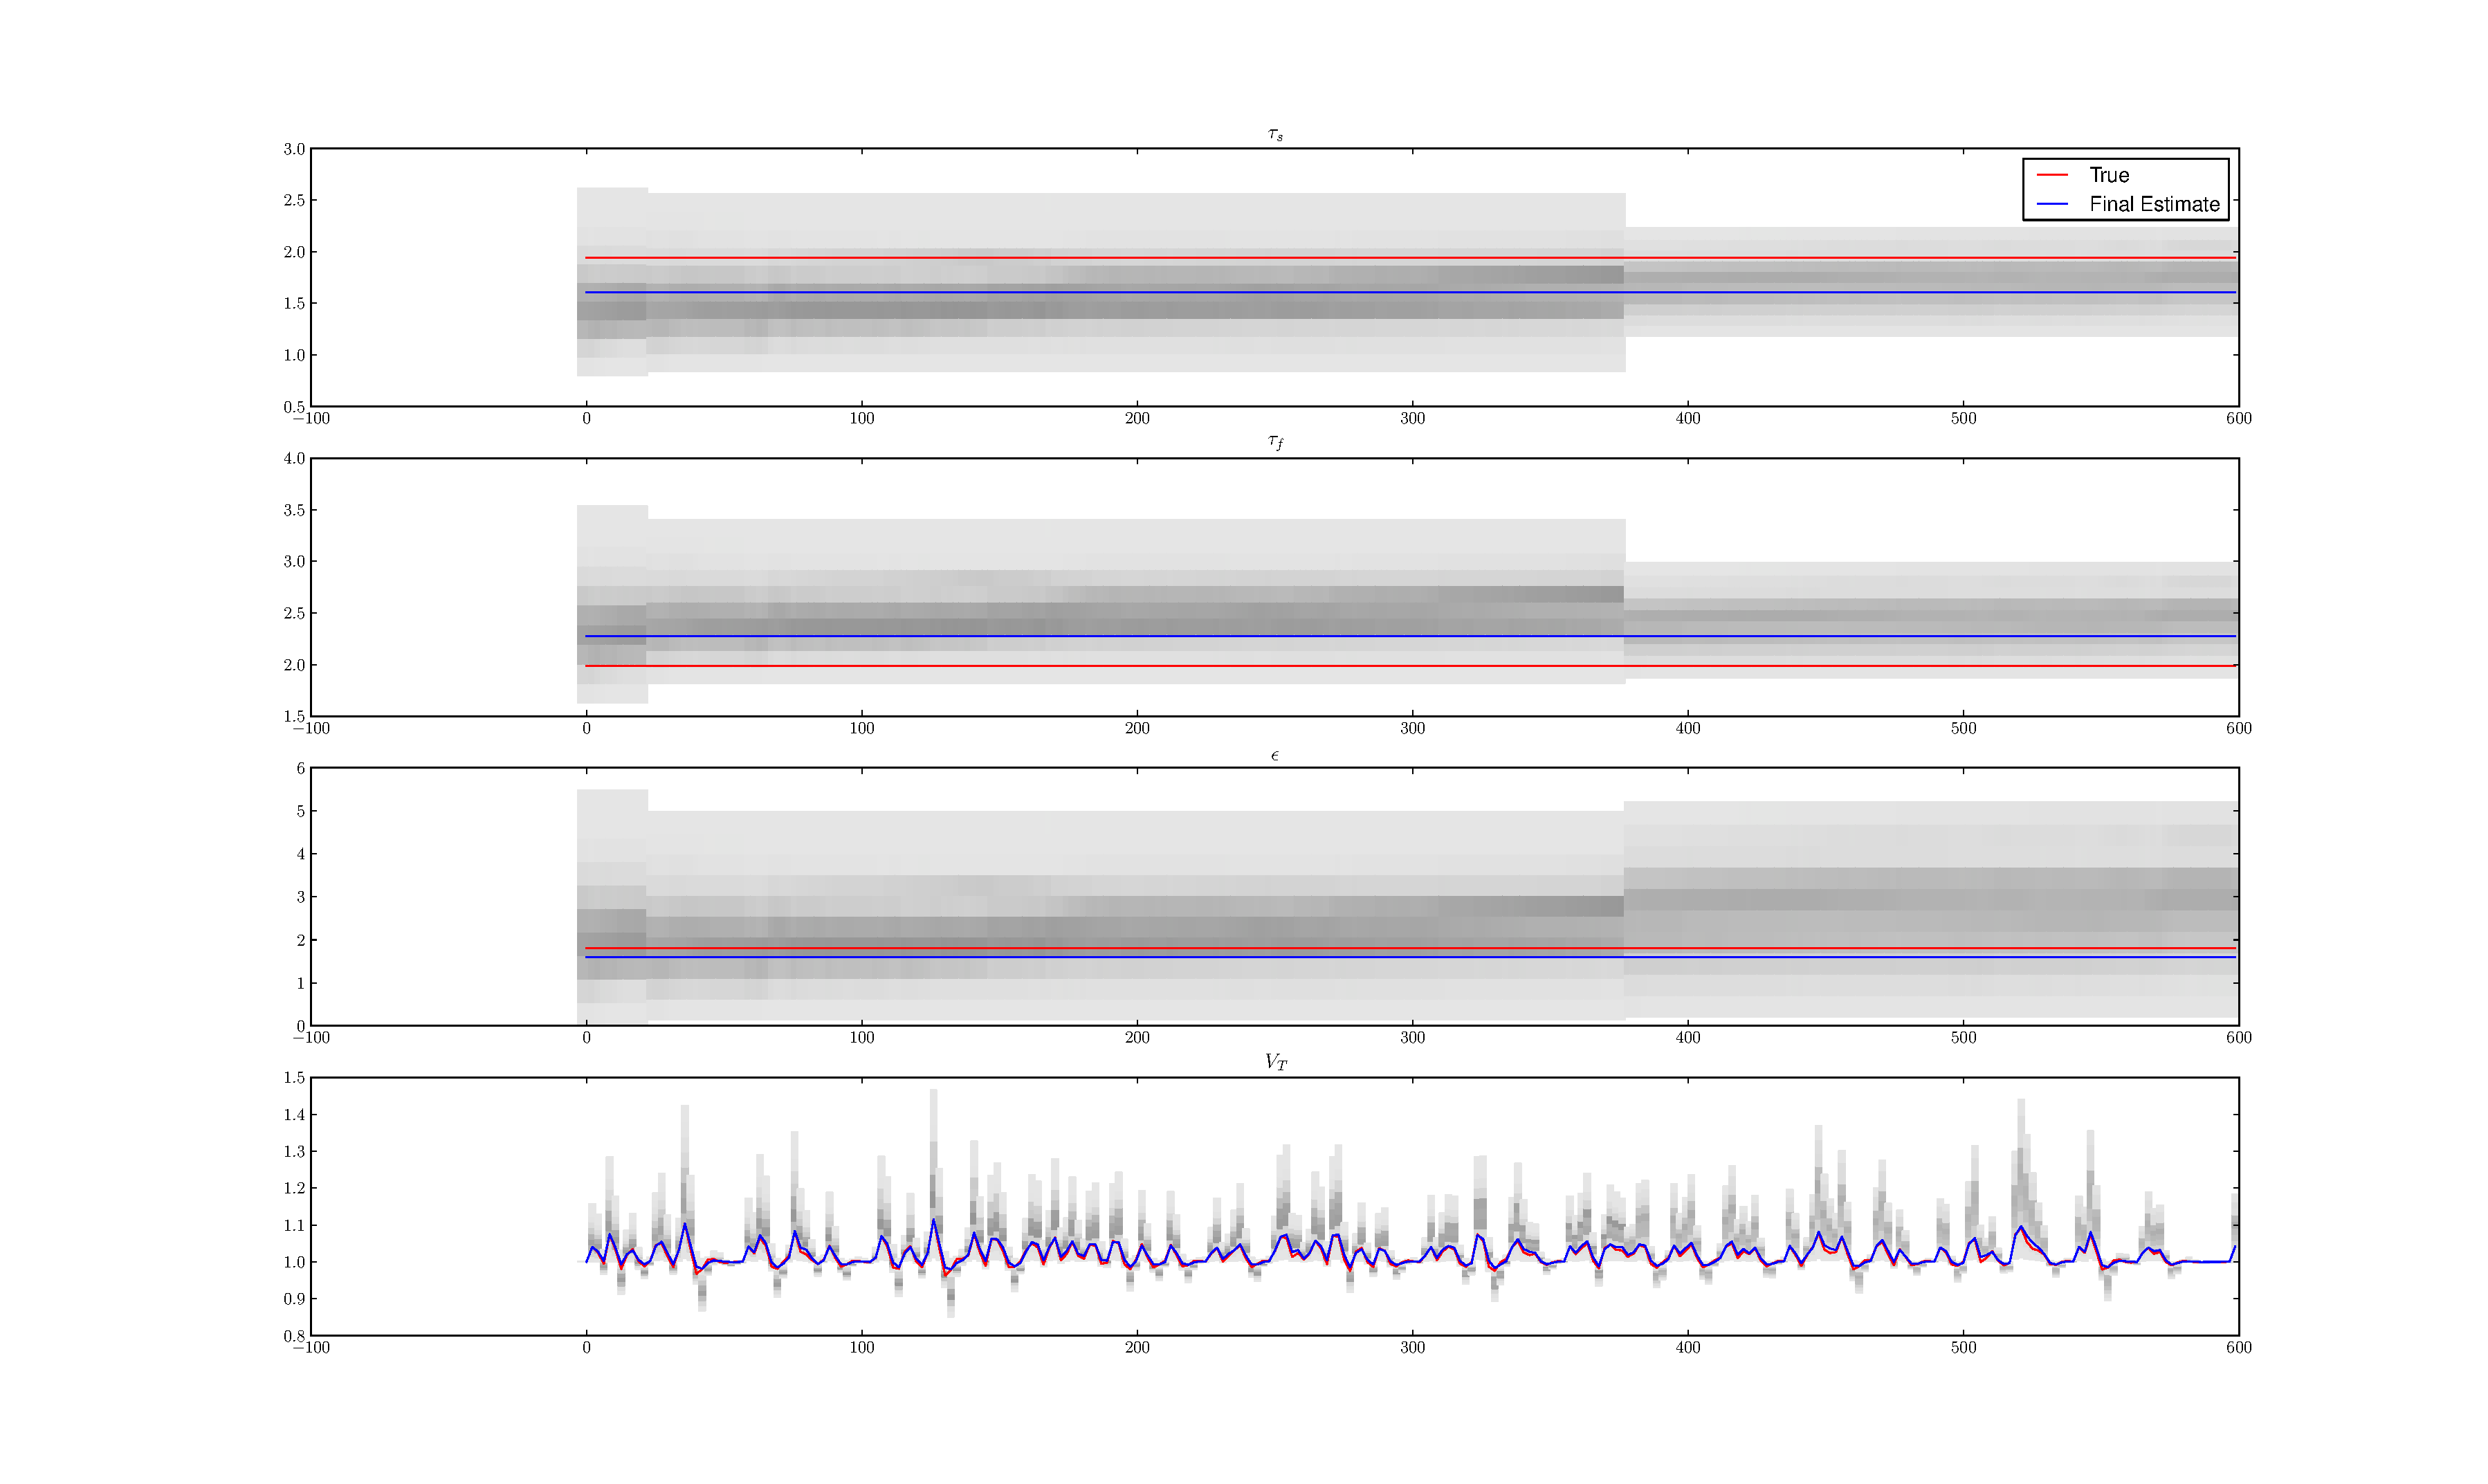
\includegraphics[trim=7cm 4cm 7cm 1cm, width=15cm]{images/converge_lownoise2}}\\
\end{figure}

\begin{figure}
\subfigure[Converging histogram for $Q$, $S$, $F$, and $BOLD$ of the first run, low noise simulation.]
{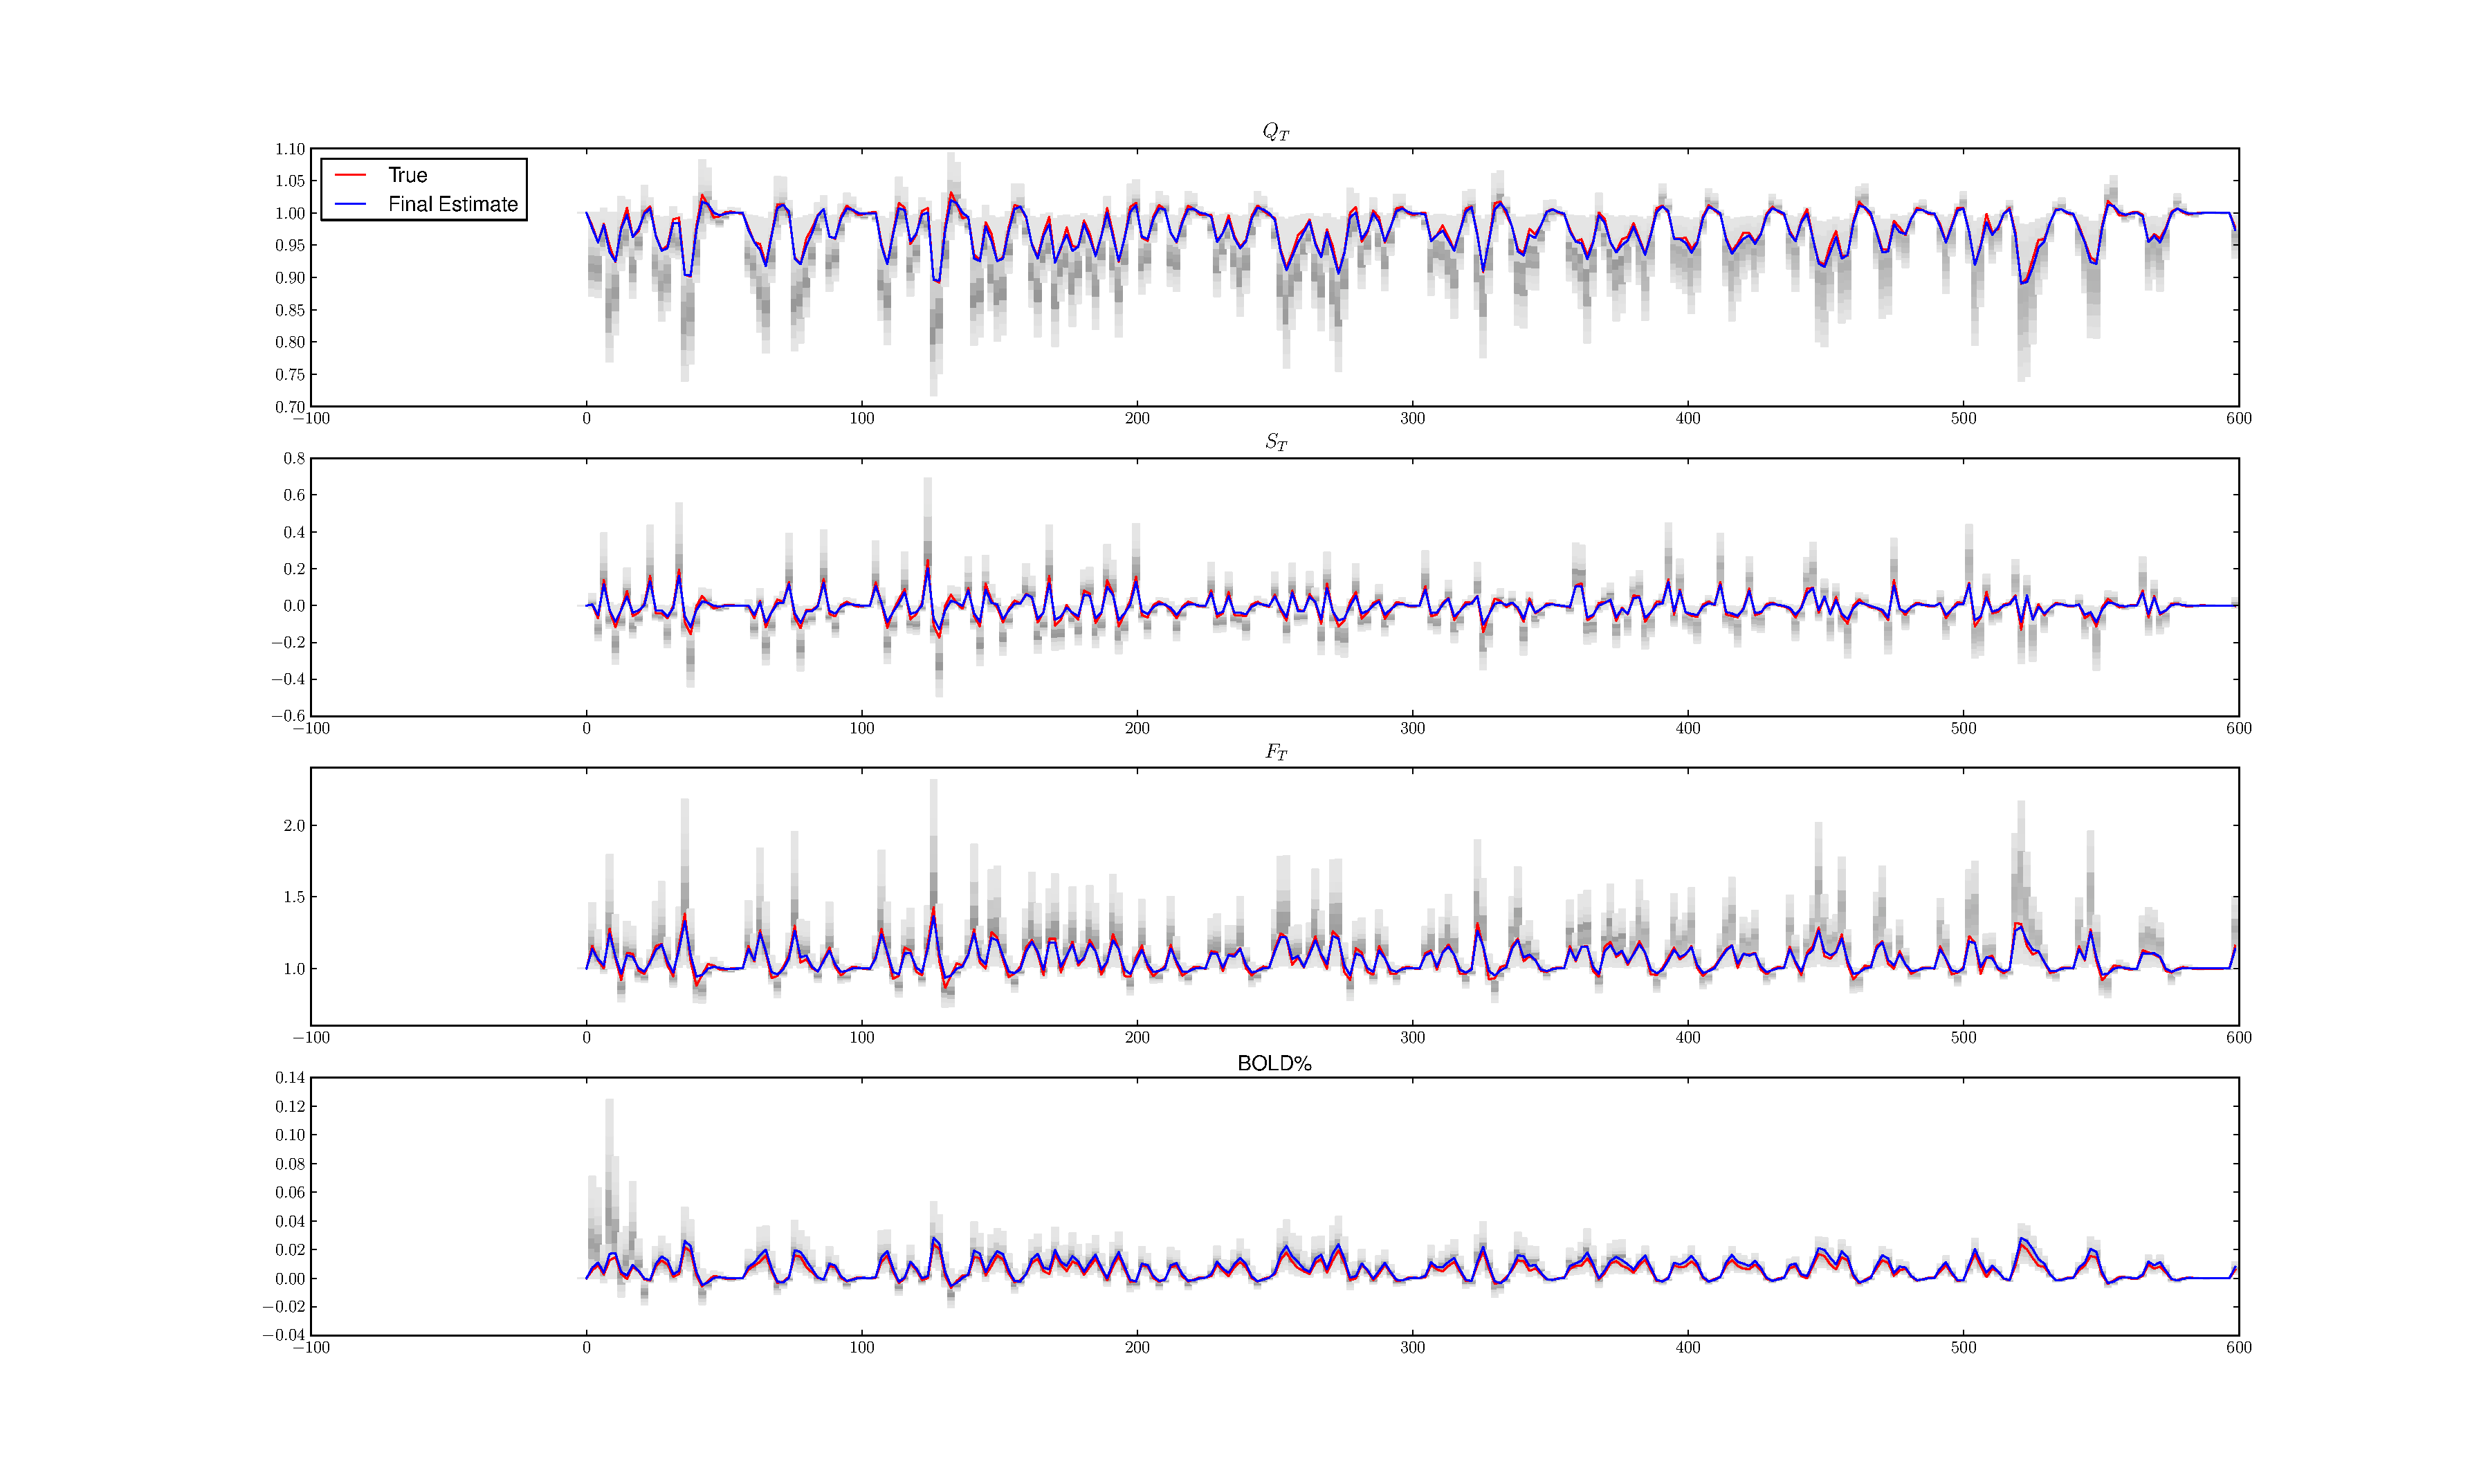
\includegraphics[trim=7cm 2cm 7cm 2cm, width=15cm]{images/converge_lownoise3}}
\label{fig:LowNoiseHist}
\end{figure}
The covariance matrix (\autoref{tab:CovSim}) also confirms the idea that the $\tau$ parameters are interchangeable
as far as the BOLD signal goes. Notice the covariance of $\tau_f$ and $\tau_0$ is $-0.019$ whereas
the variance of $\tau_0$ and $\tau_f$ are $0.019$ and $0.04$ respectively. Clearly they are
related. The convergence properties of the first run in \autoref{tab:LowNoiseResults} may be
viewed in \autoref{fig:LowNoiseHist}.

\subsubsection{High Noise Simulation}
For the high noise simulation, the exact same procedure was performed again, but with 
measurement error and drift standard
deviations an order of magnitude higher. The noisy signals versus the base signal are shown
in \autoref{fig:HighNoiseRealization} and the preprocessed signals which the particle
filter attempt to fit are in \autoref{fig:PreprocessedHighNoise}.
\begin{figure}[H]
\label{fig:LowNoiseRealization}
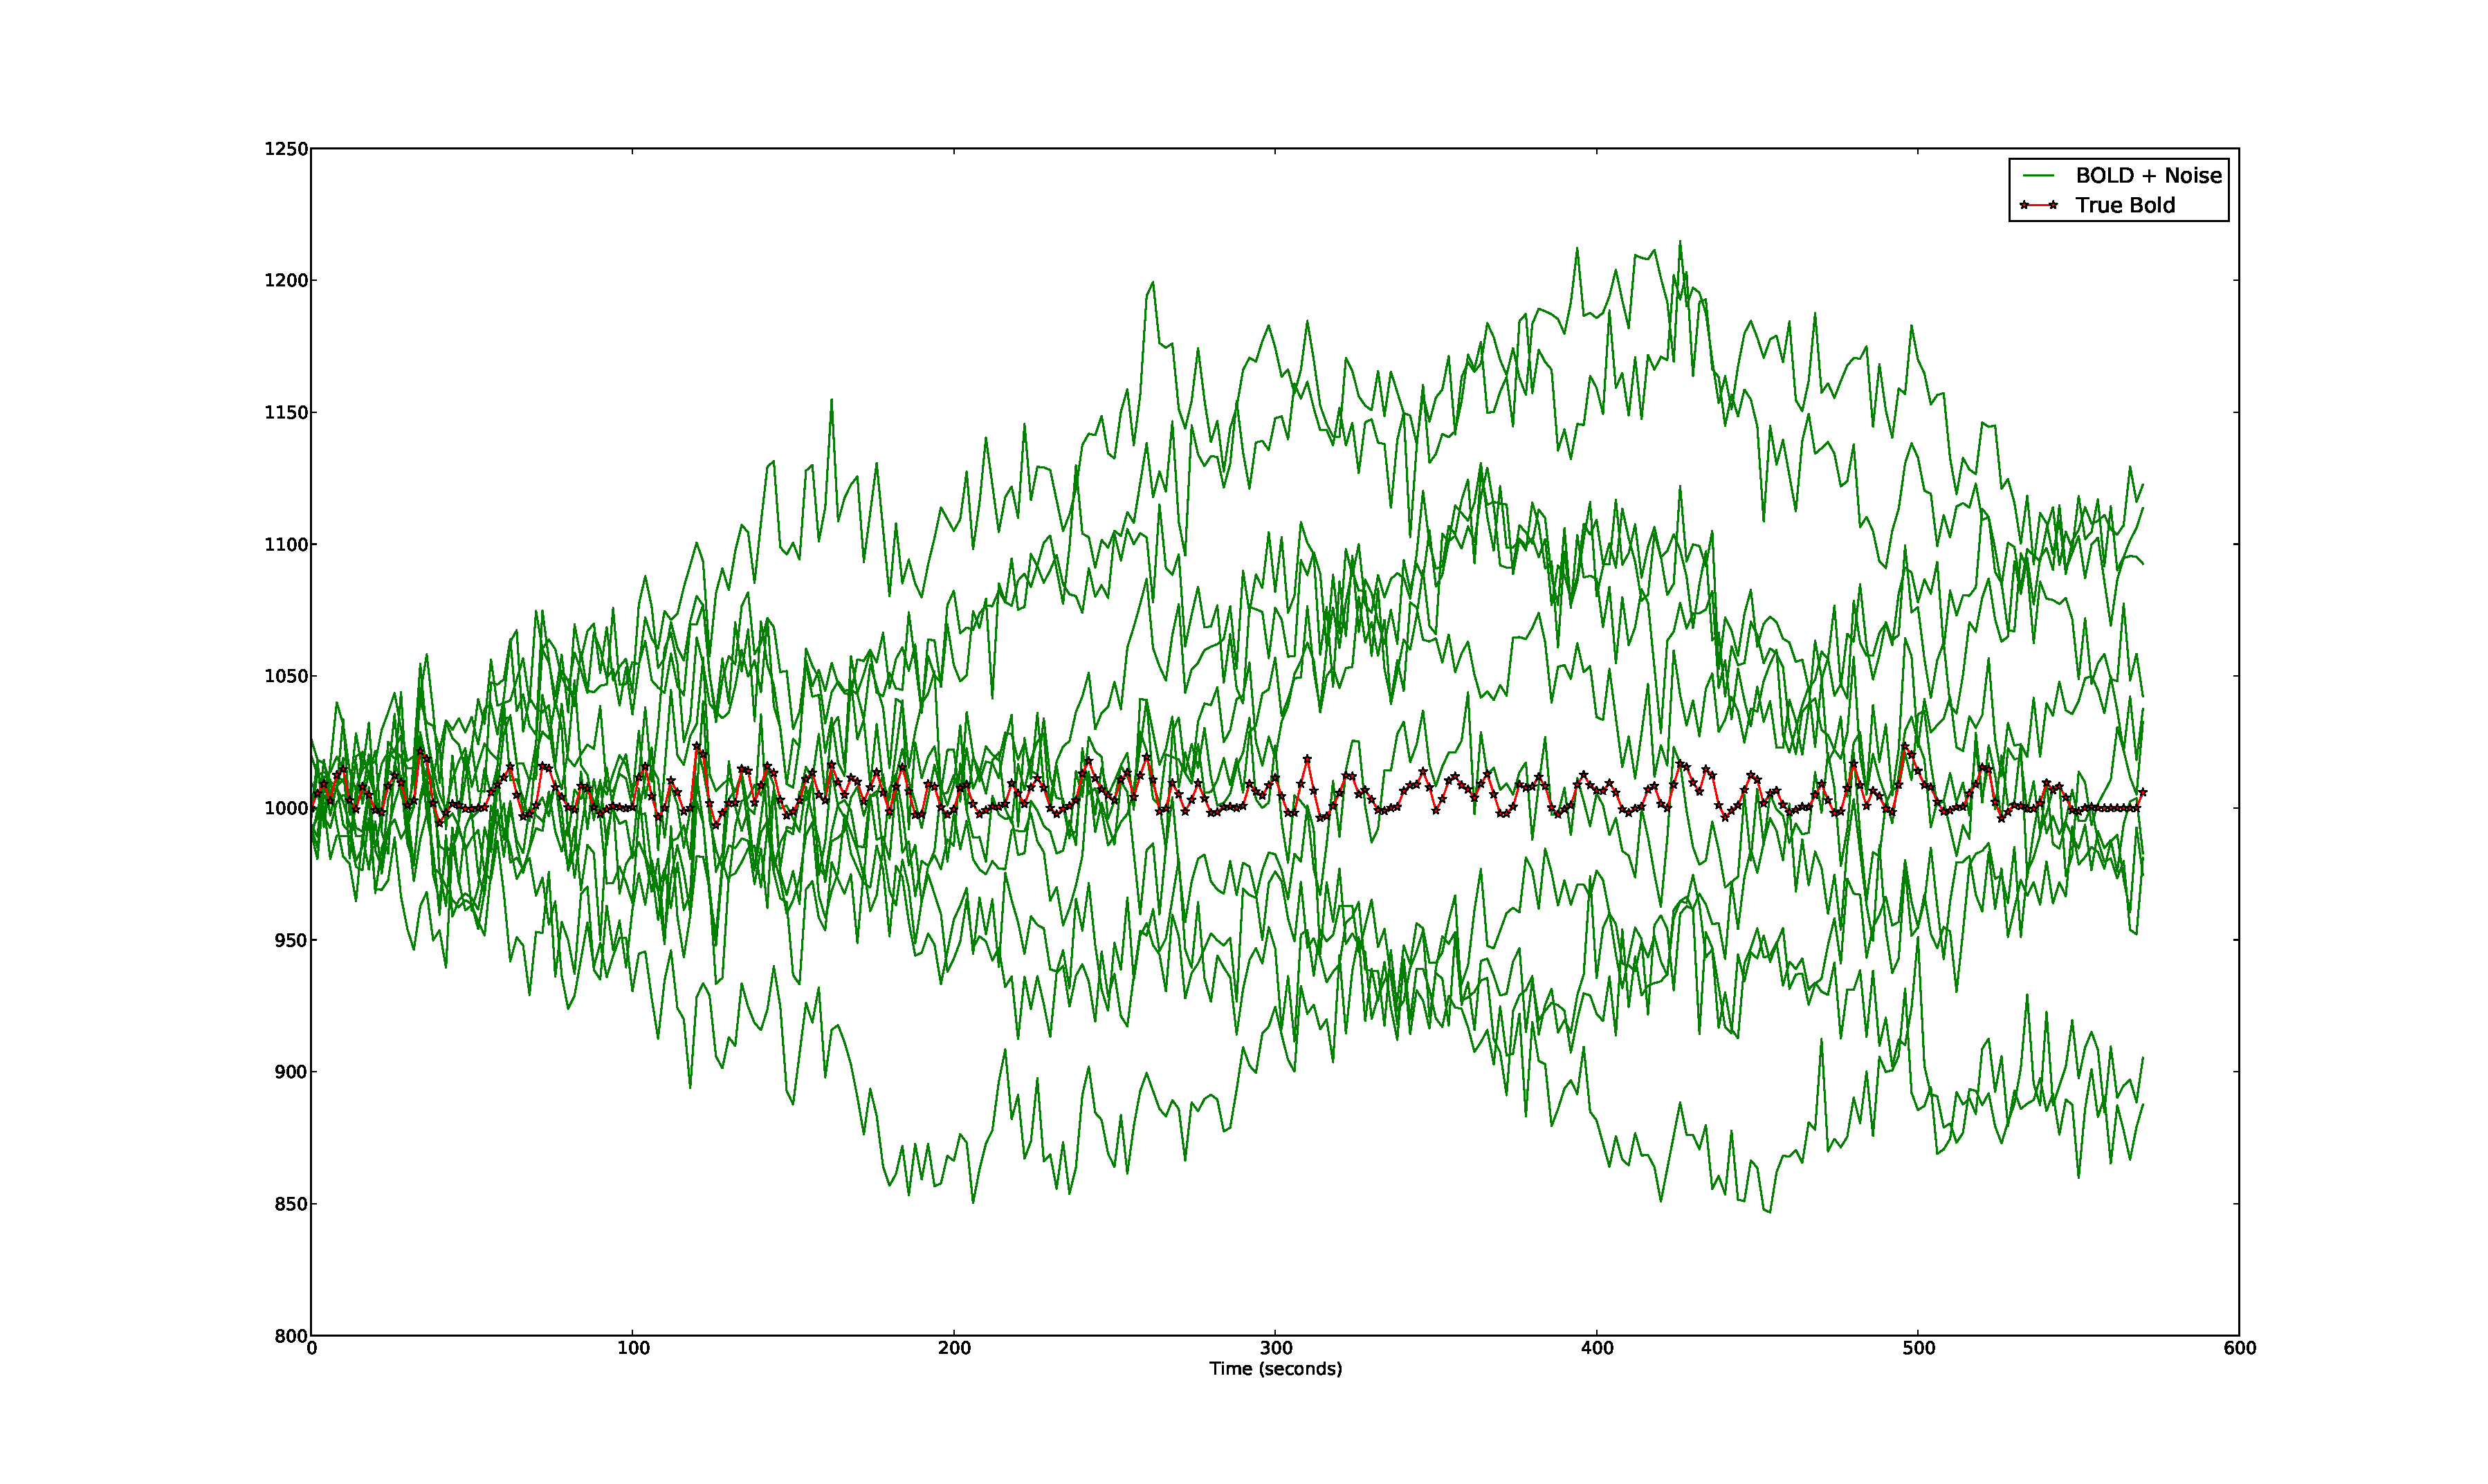
\includegraphics[trim=6cm 3cm 6cm 3cm,width=16cm]{images/realization_highnoise}
\caption{Test Signals with high noise compared to the clean signal, $\sigma_x = .01, \sigma_y=.005$}
\end{figure}
\begin{figure}[H]
\label{fig:PreprocessedHighNoise}
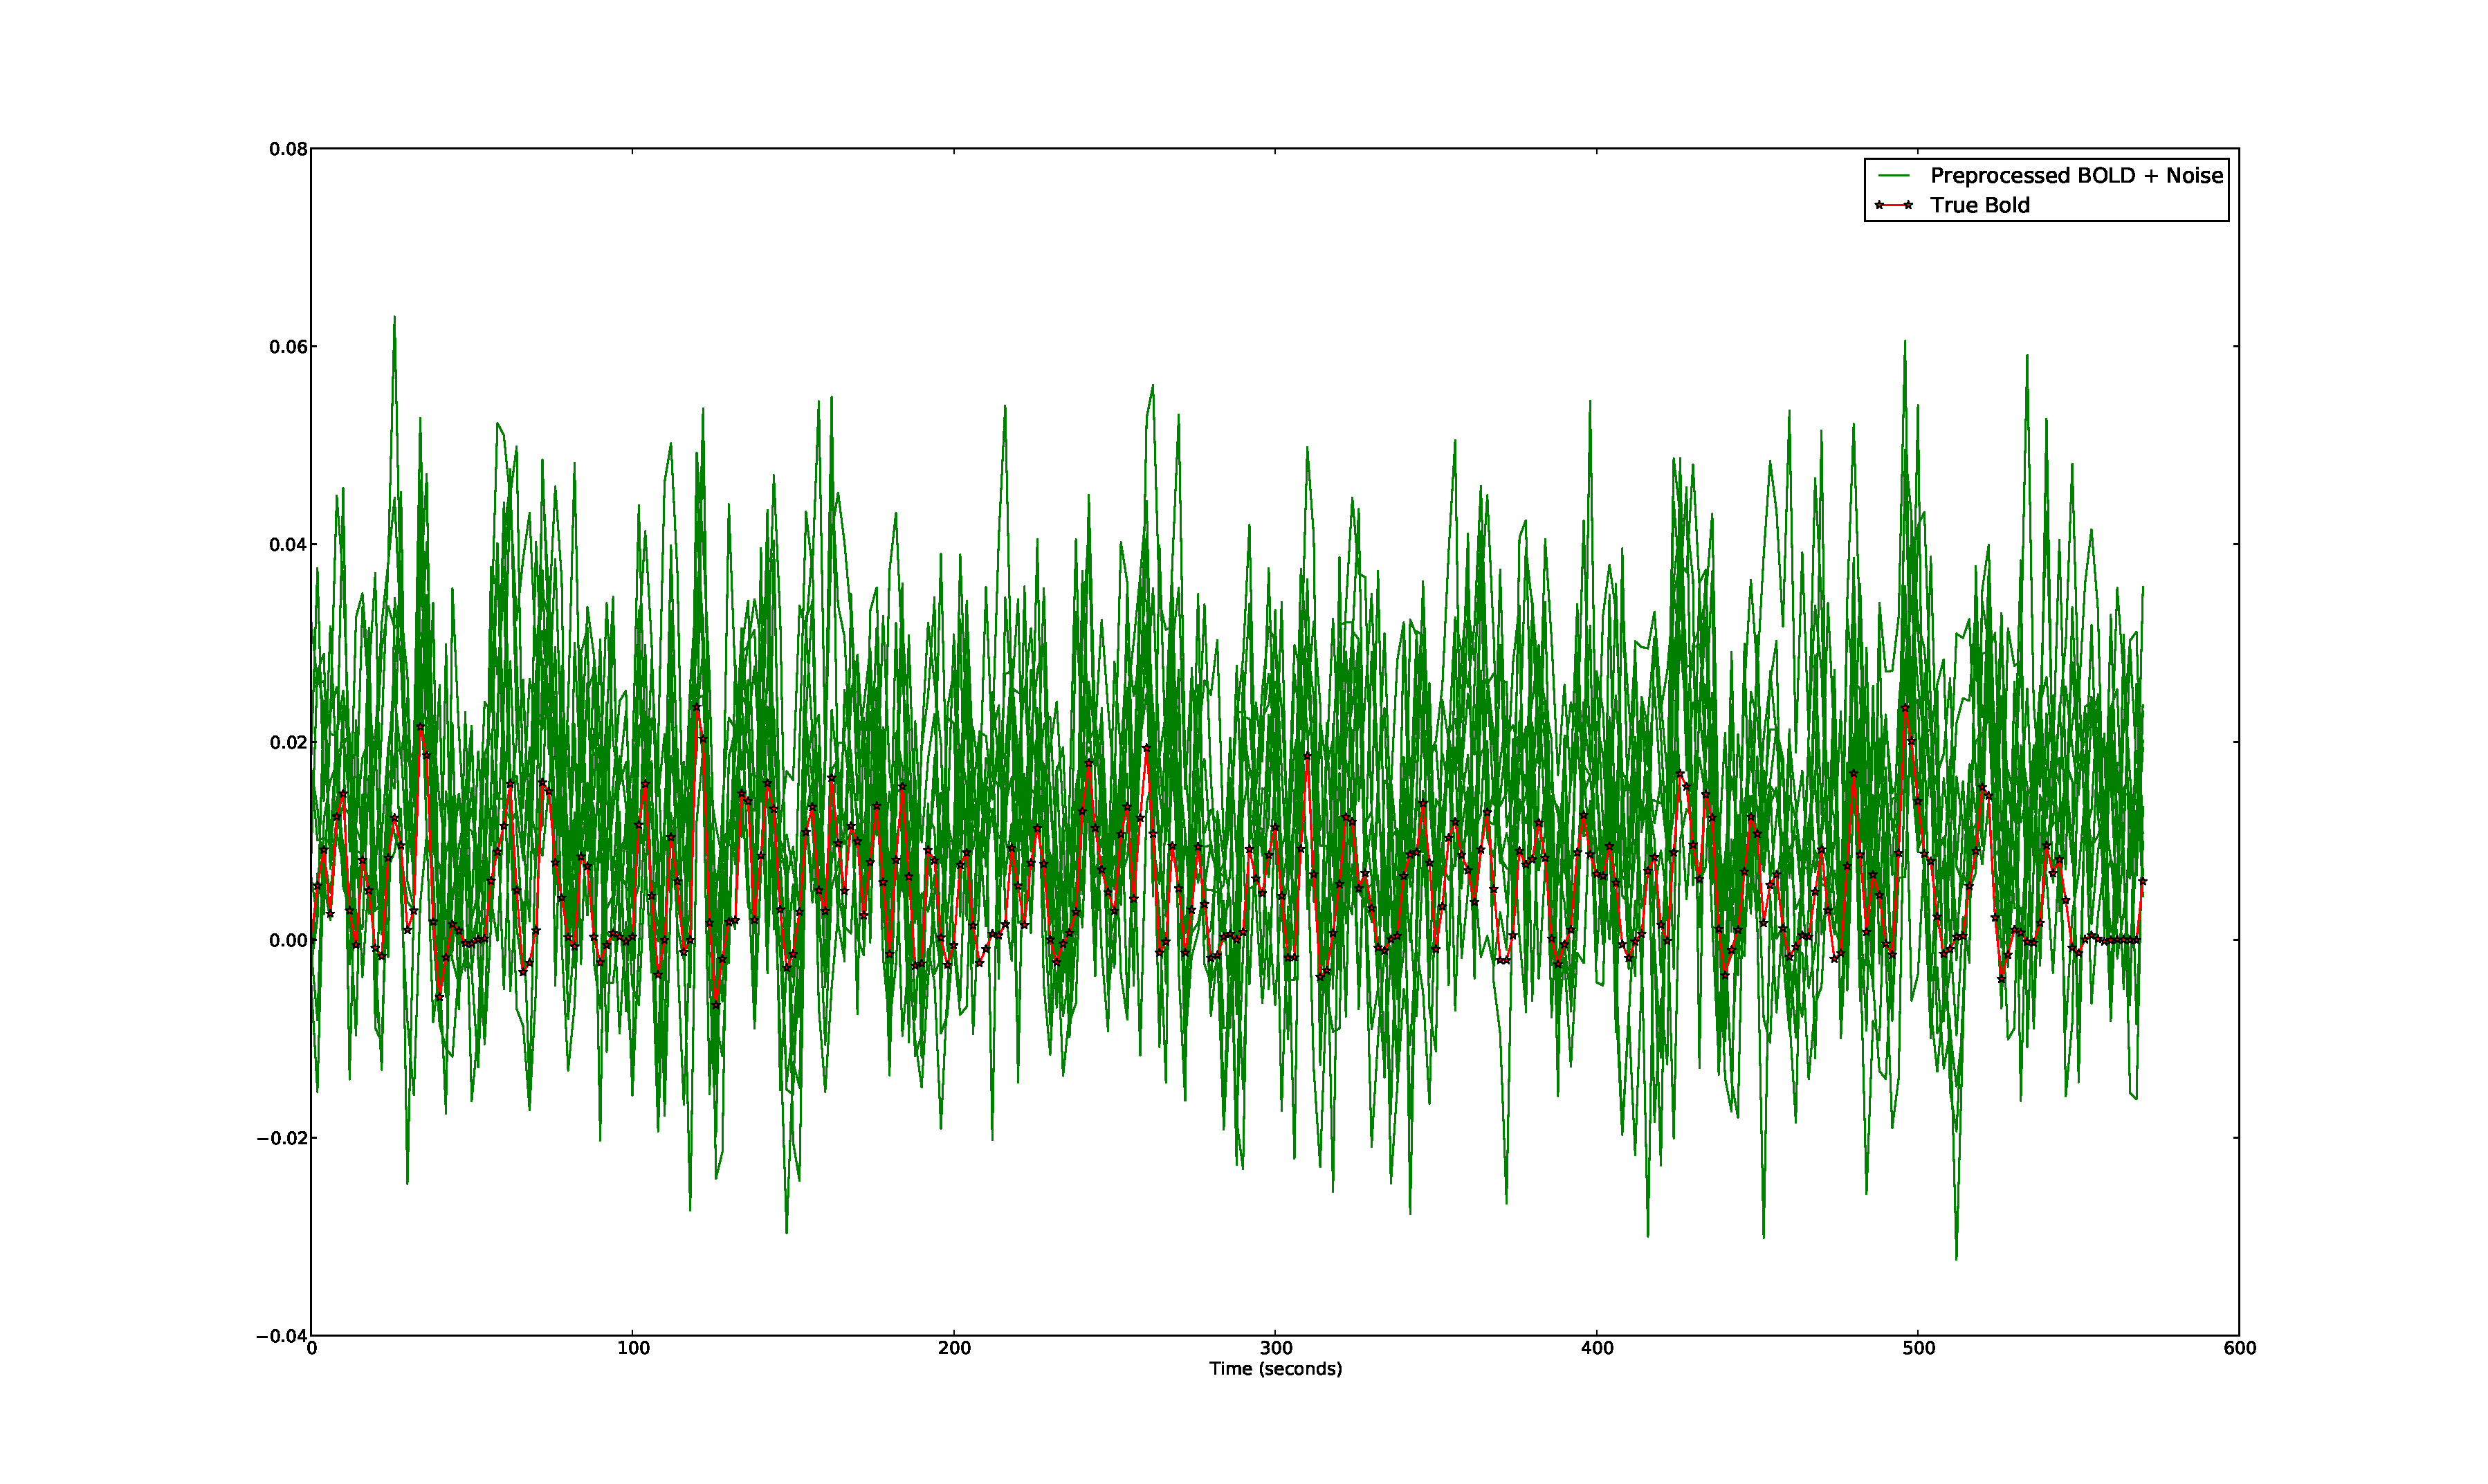
\includegraphics[trim=6cm 3cm 6cm 3cm,width=16cm]{images/preprocessed_highnoise}
\caption{A comparison of the preprocessed signals for the high noise case.}
\end{figure}

The results of the particle filter, for each of the ten runs may be seen in 
\autoref{fig:FitComparisonHighNoise}. Clearly the preprocessing led the algorithm
to somewhat higher activation levels, and it would appear that the subtleties of
different time constants are also lost for most of the runs, although a few seem
to manage quite accurate results. 

\begin{figure}[H]
\label{fig:FitComparisonHighNoise}
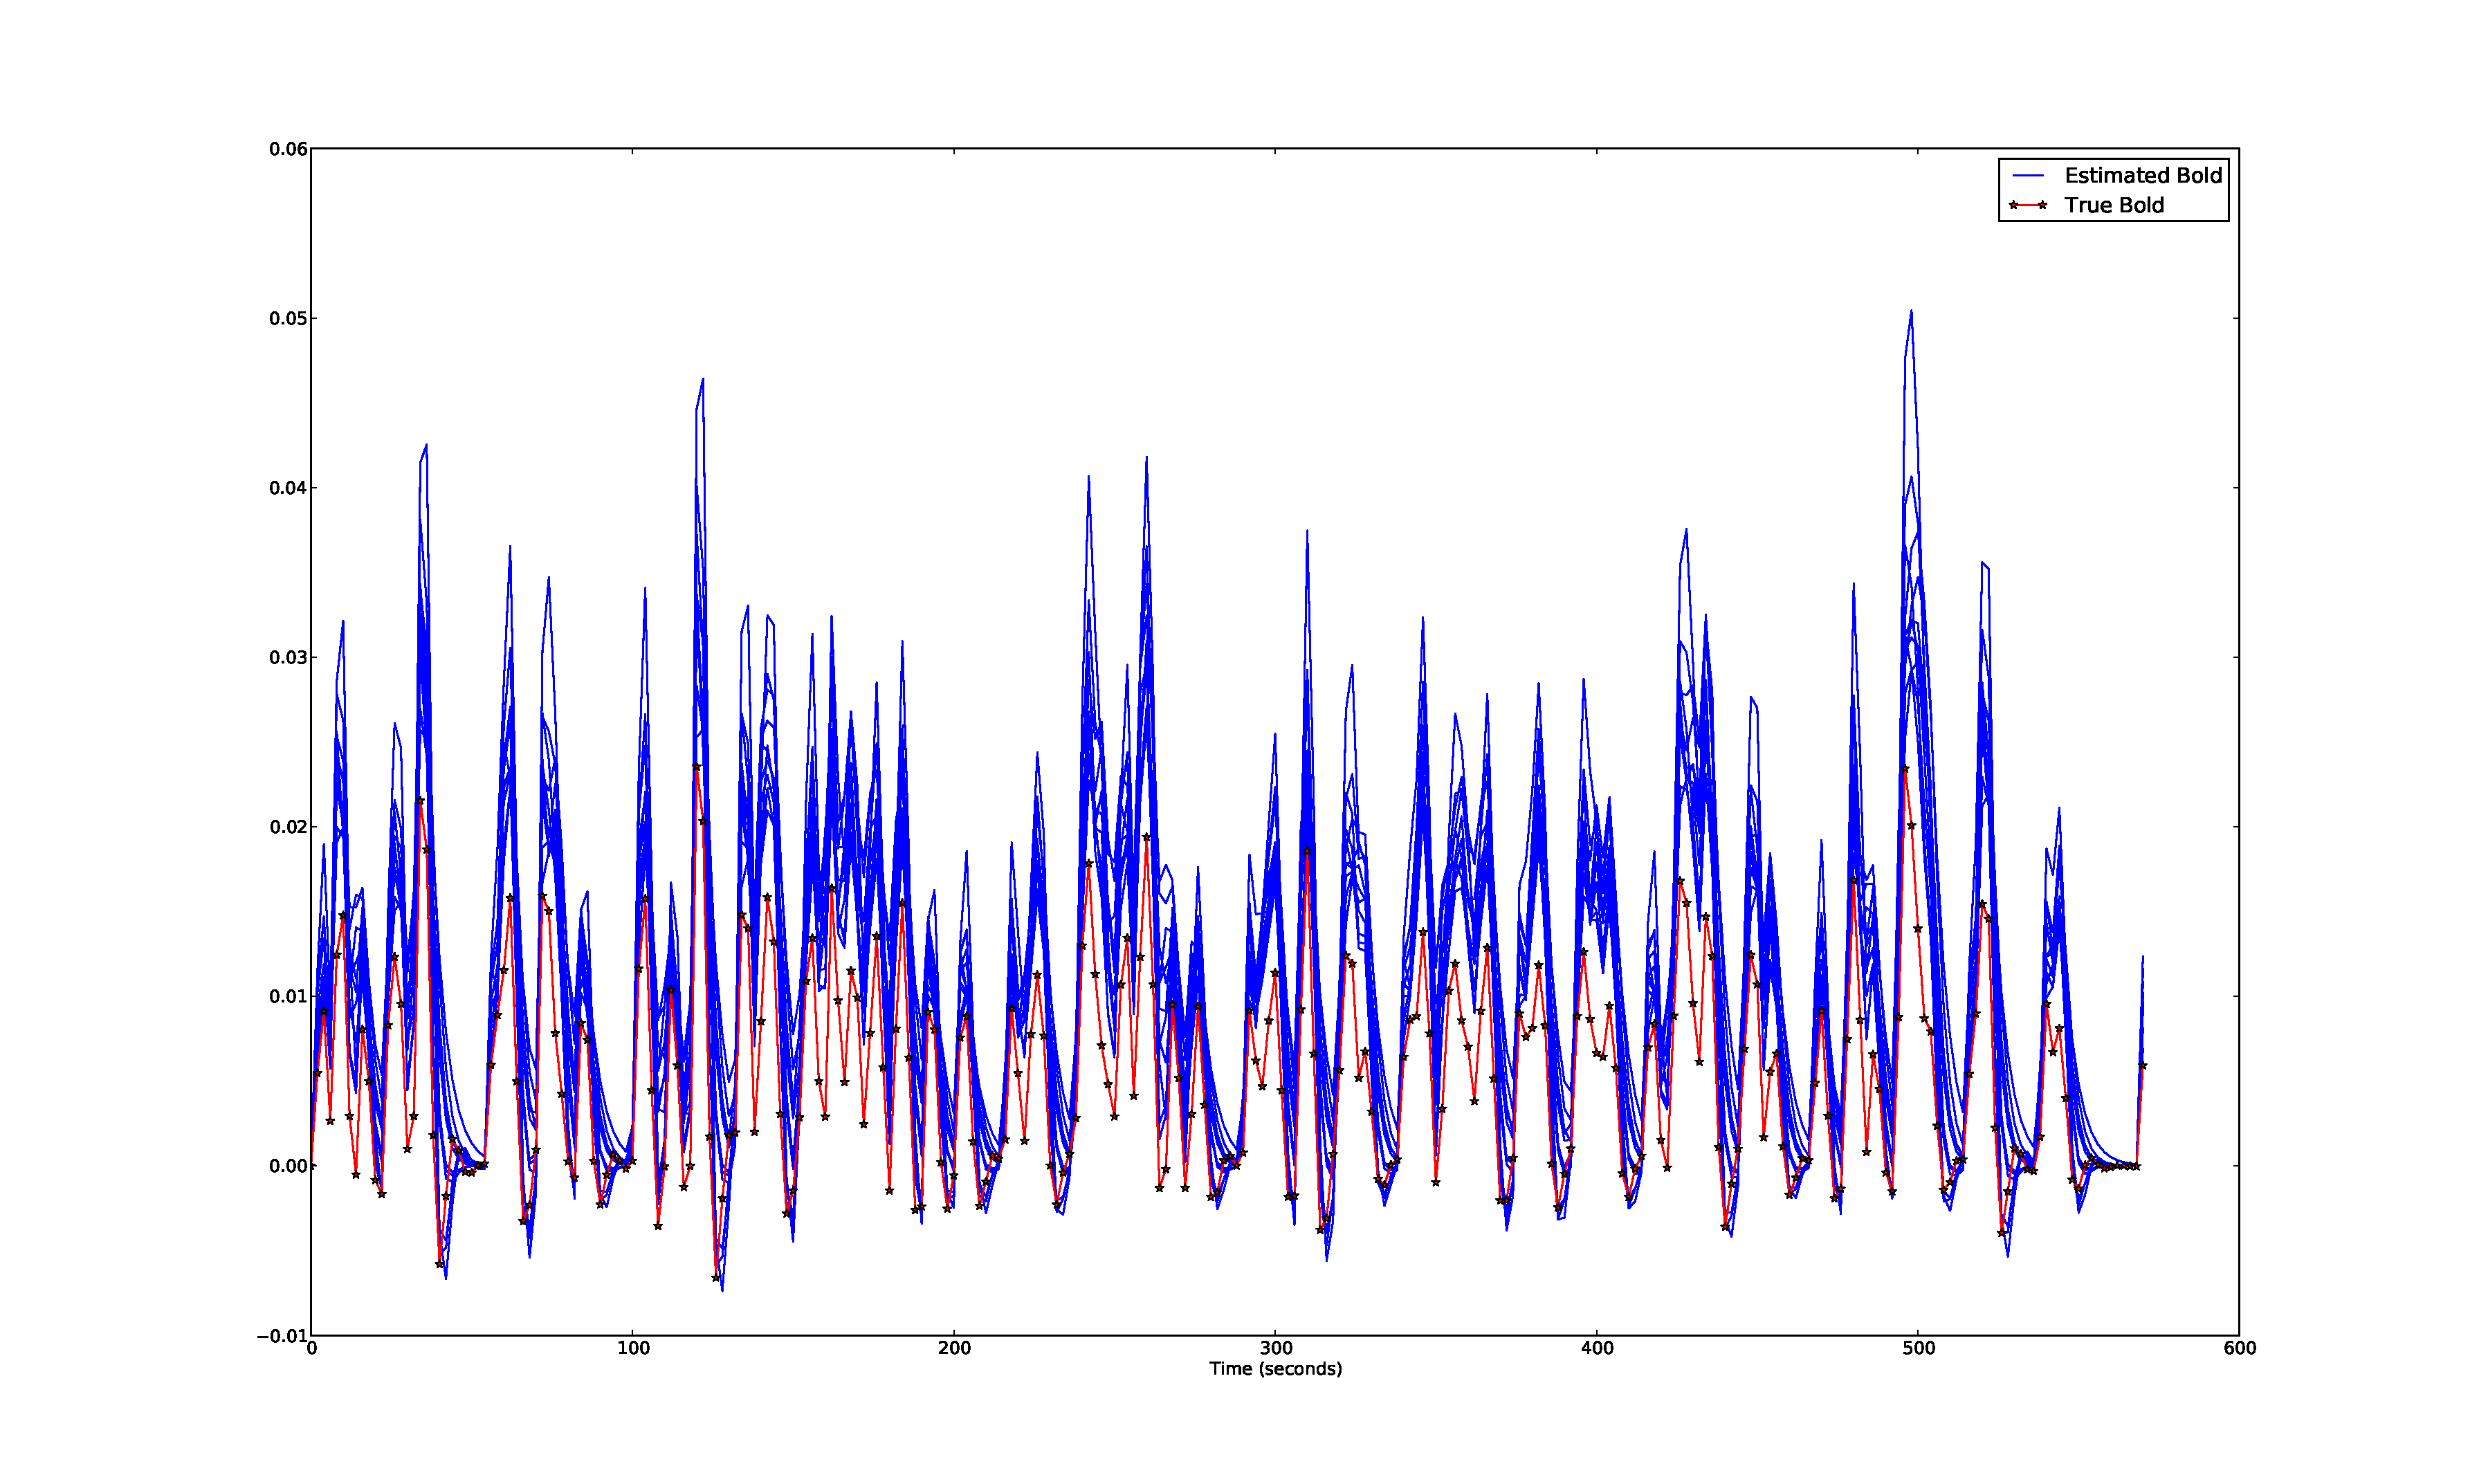
\includegraphics[trim=6cm 3cm 6cm 3cm,width=16cm]{images/comparison_highnoise}
\caption{A comparison of the fitted signals for the high noise case.}
\end{figure}
\begin{figure}[H]
\label{fig:NoiseComparisonJustTwo}
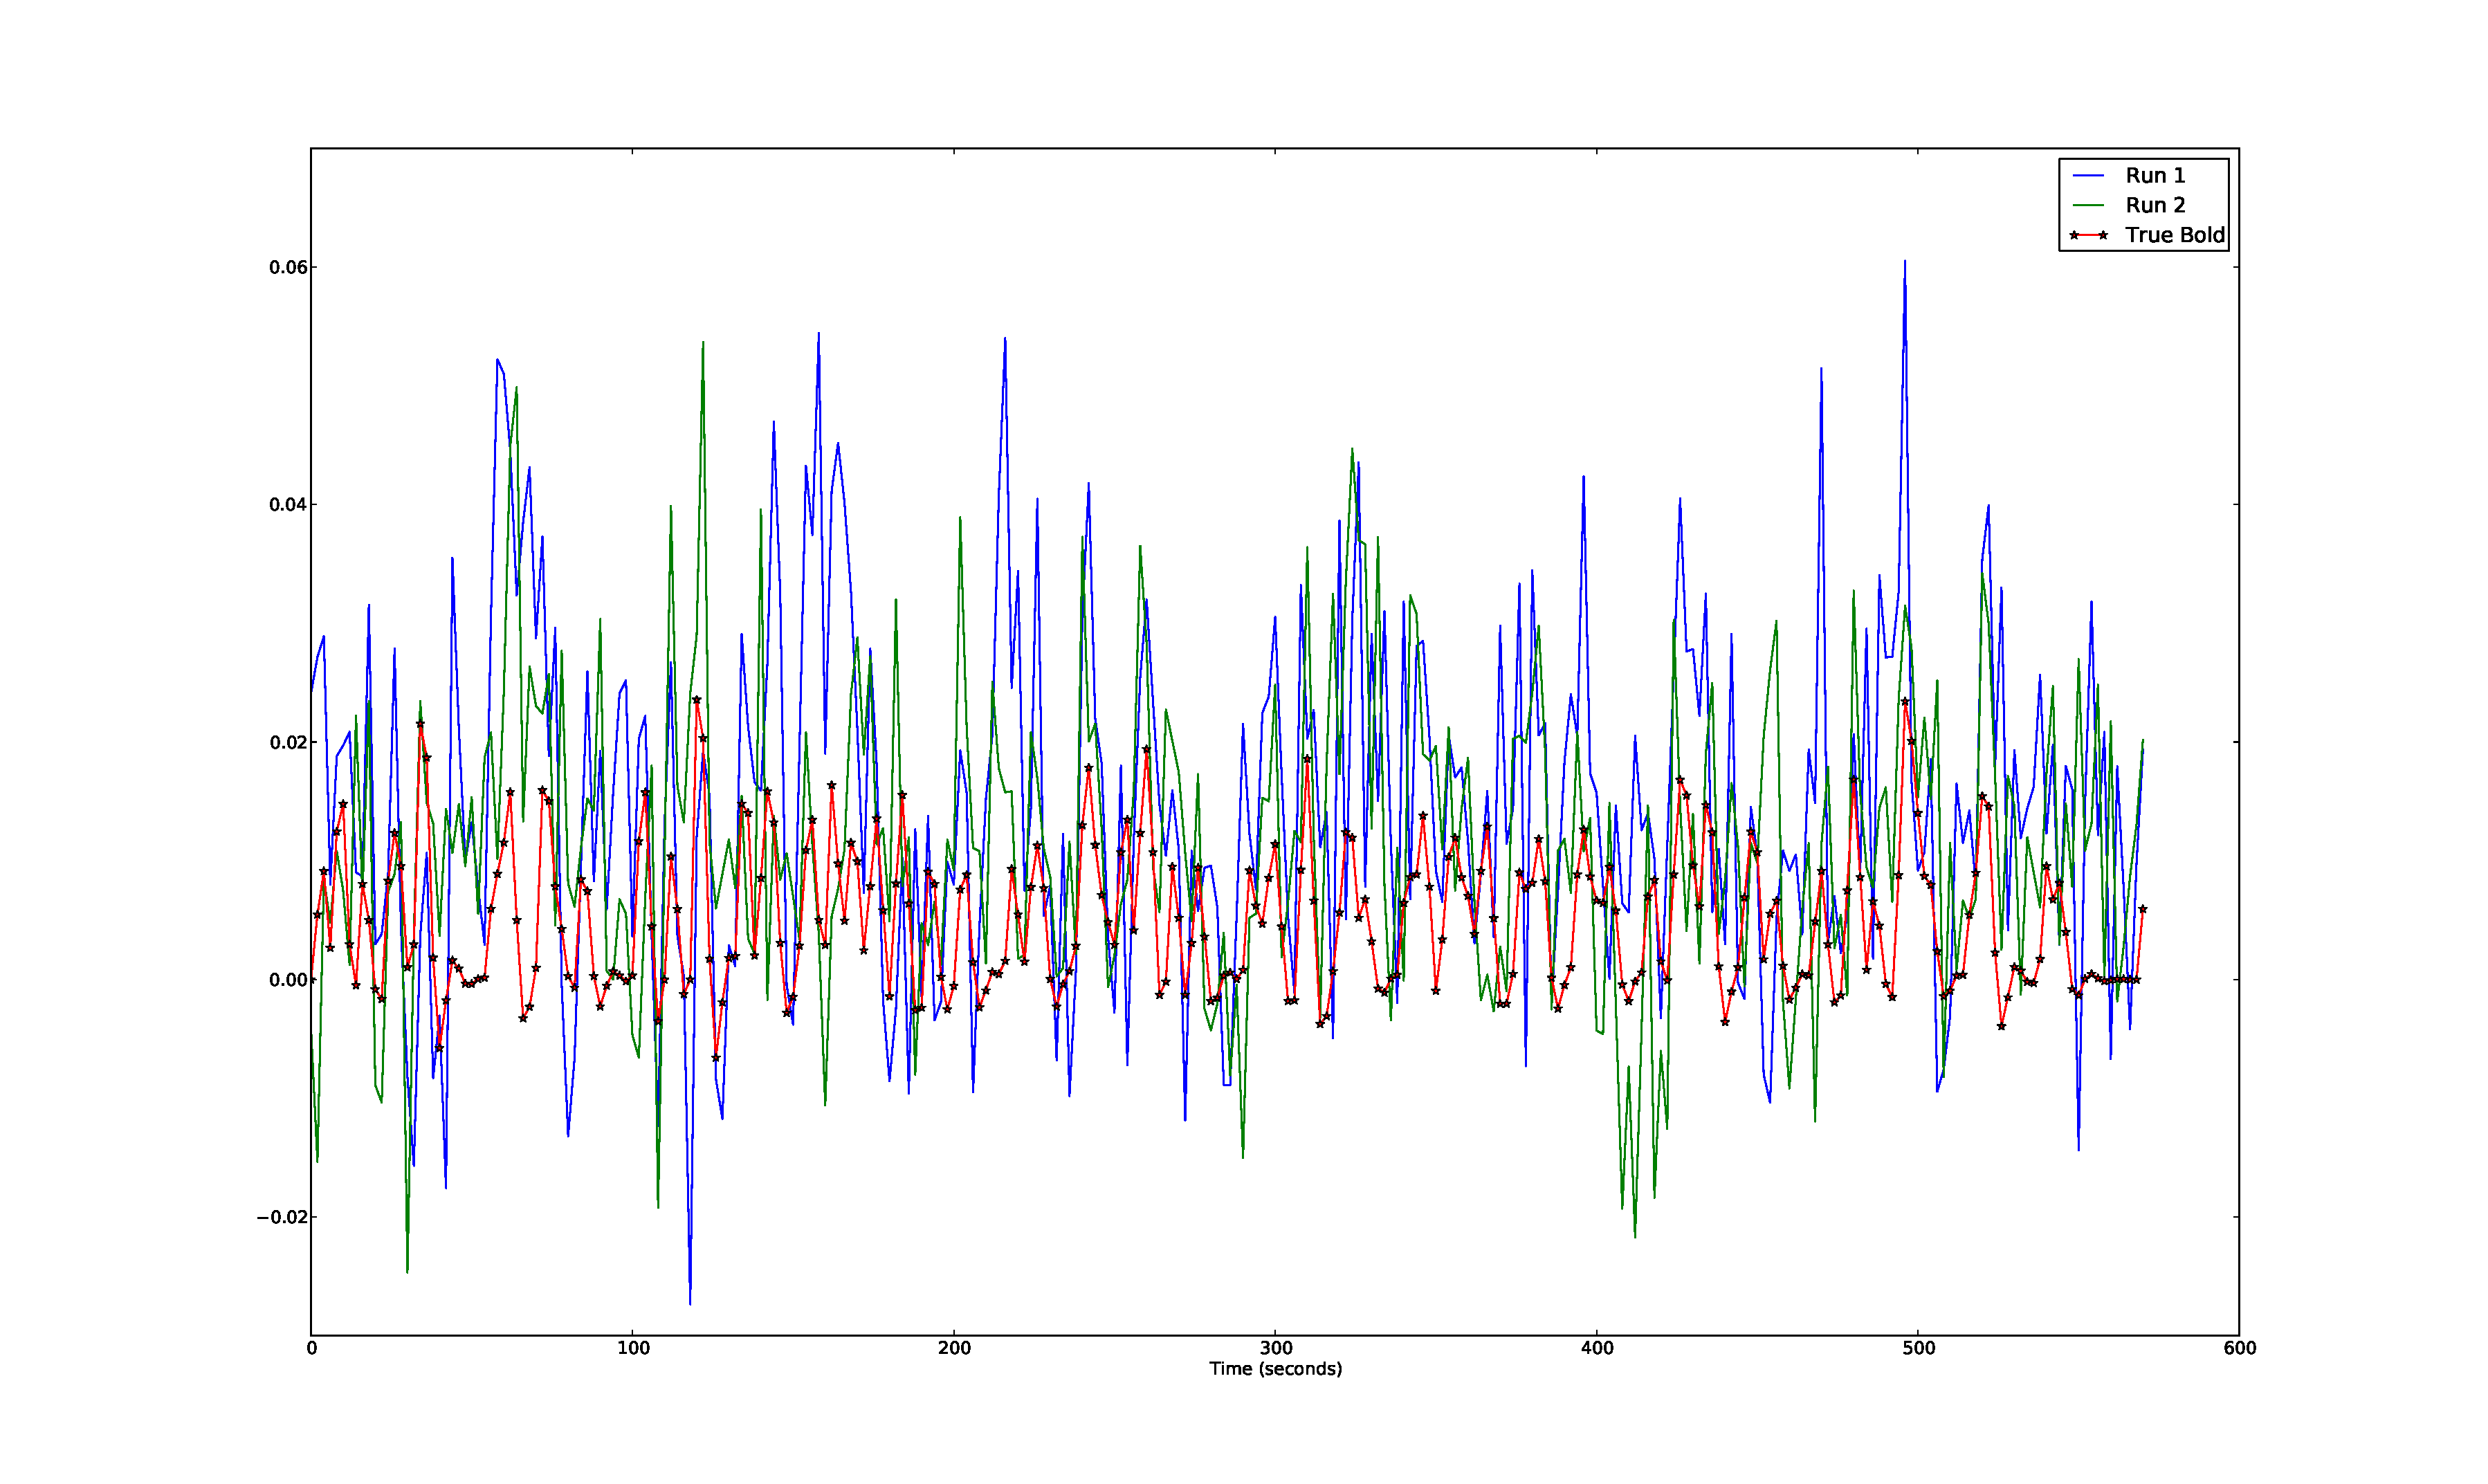
\includegraphics[trim=6cm 3cm 6cm 3cm,width=16cm]{images/highnoise_56_noise}
\caption{Two particular preprocessed noise realizations for the high noise case.}
\end{figure}
\begin{figure}[H]
\label{fig:FitComparisonHighNoiseJust2}
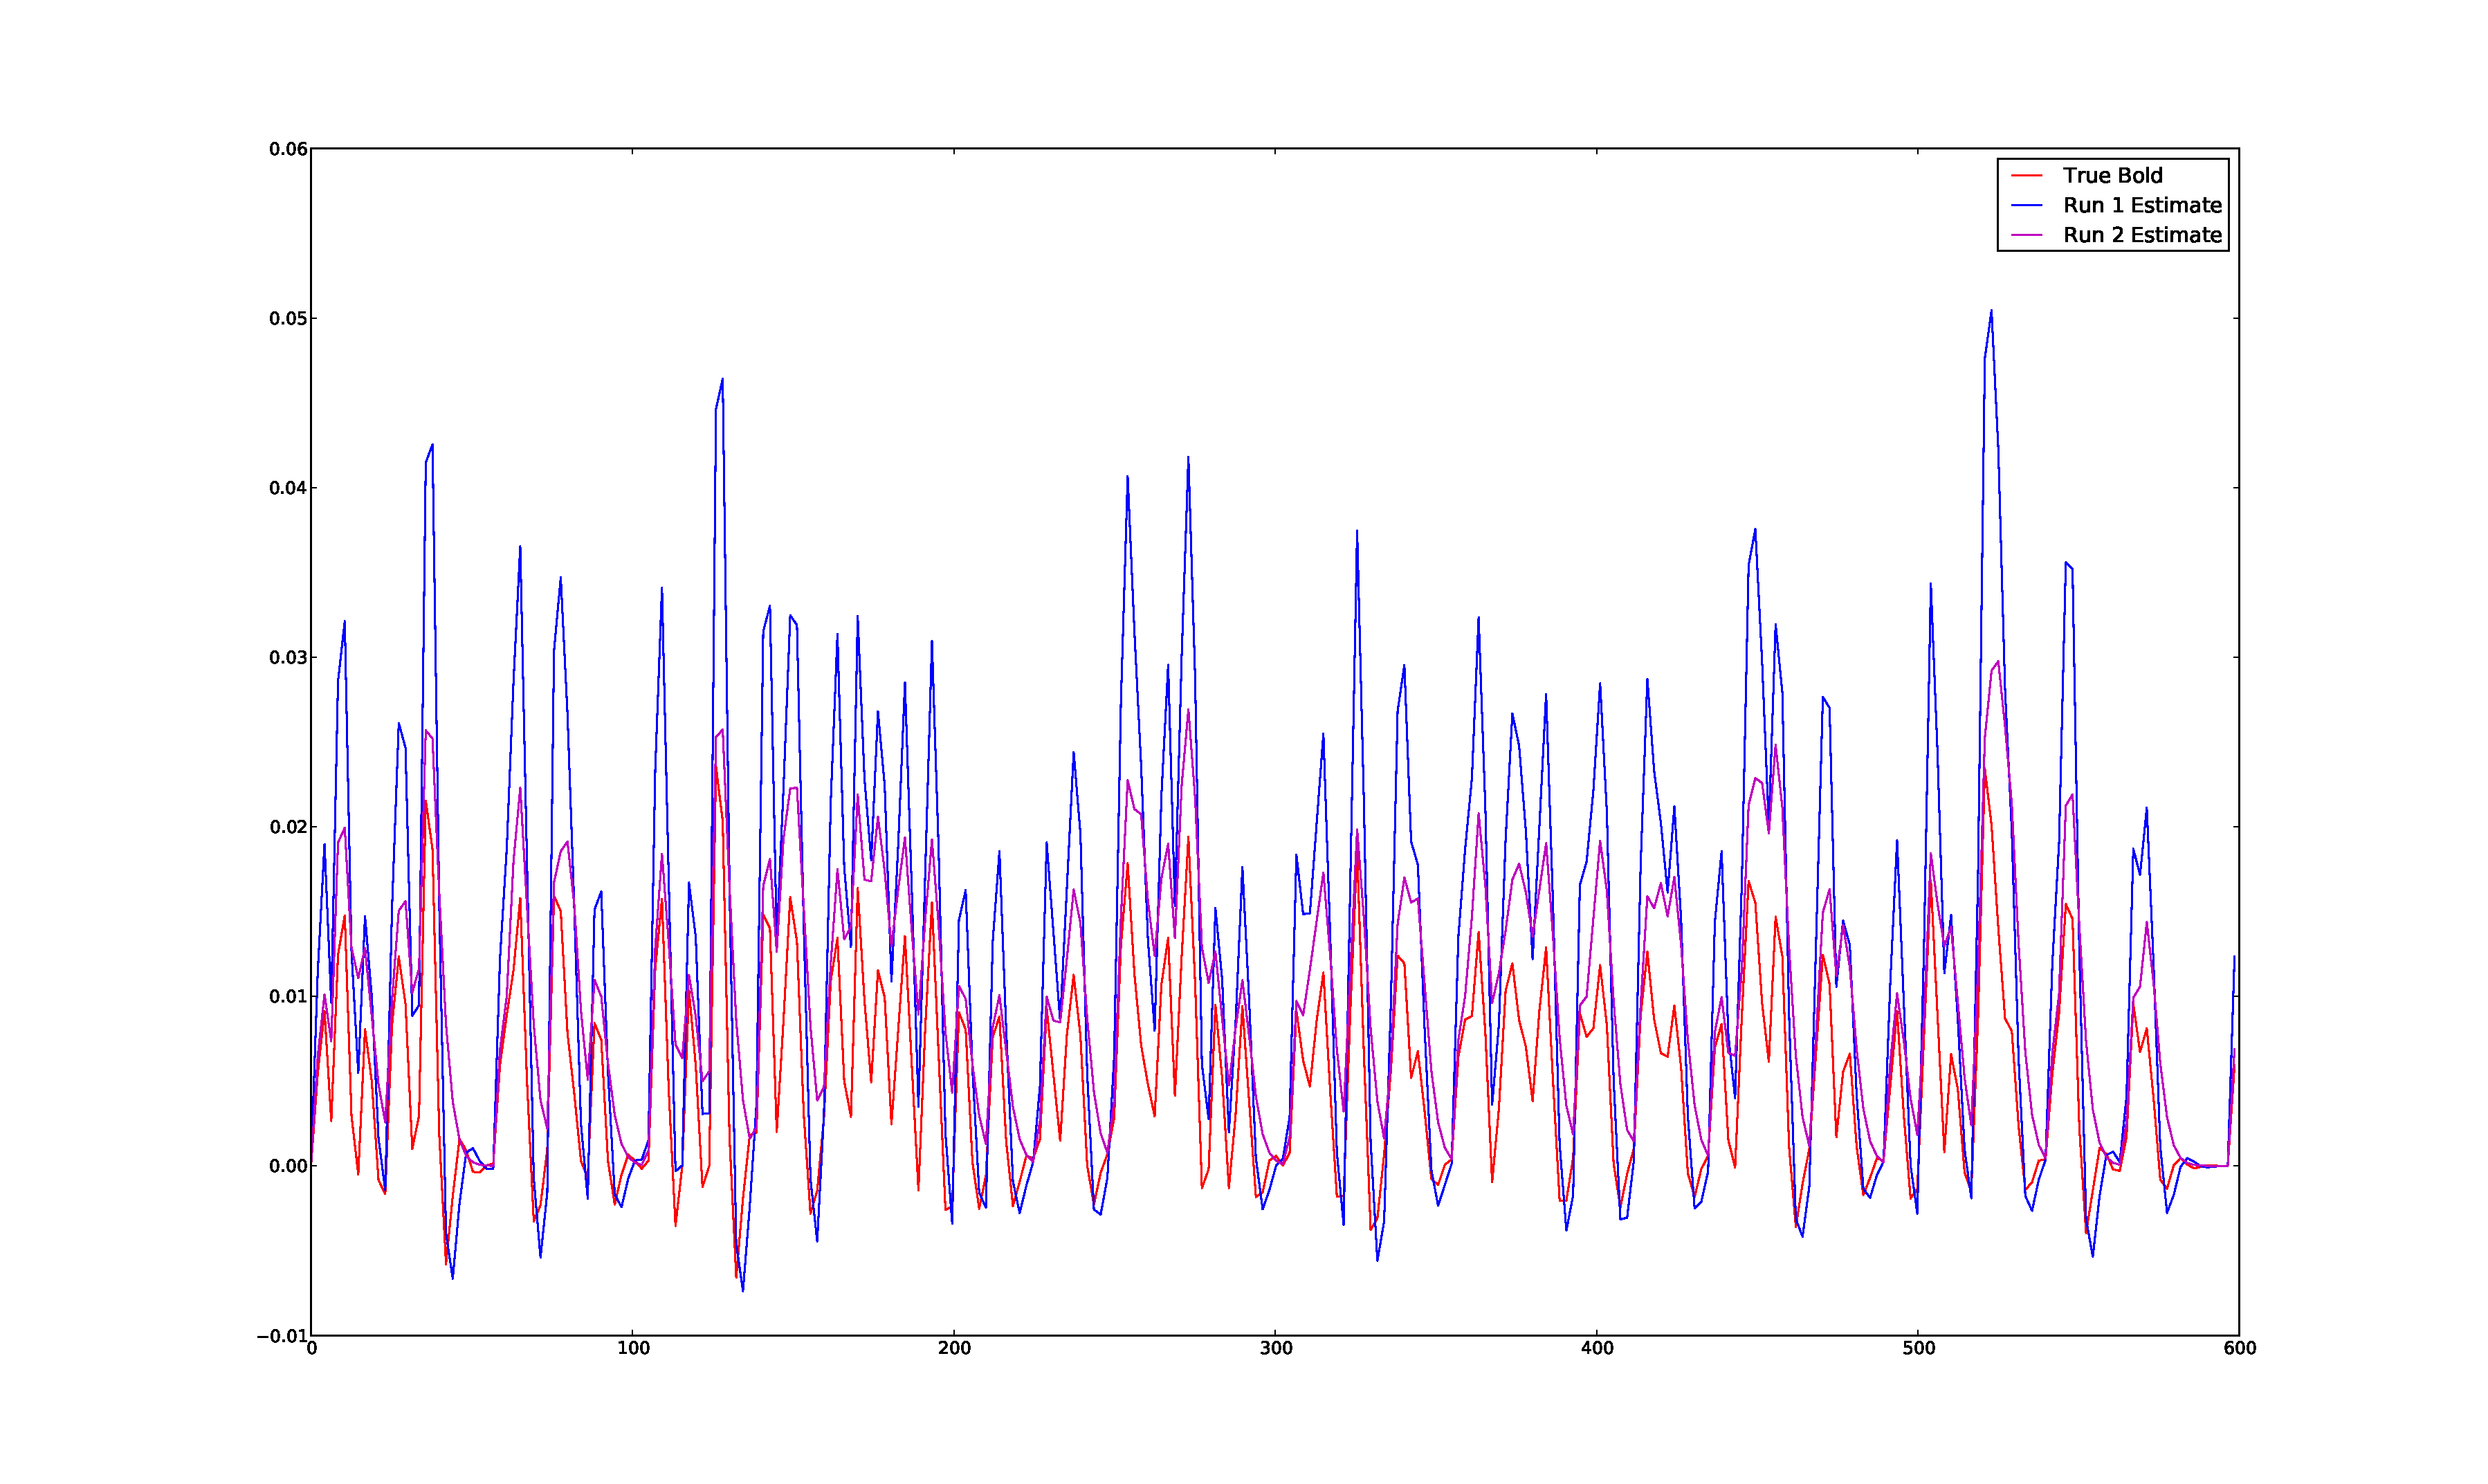
\includegraphics[trim=6cm 3cm 6cm 3cm,width=16cm]{images/comparison_highnoise_just2}
\caption{The results for the noise realizations shown in \autoref{fig:NoiseComparisonJustTwo}.}
\end{figure}

It is interesting to consider how the preprocessing and noise may effect the
parameters of the fitting model. For instance run 1 in \autoref{fig:NoiseComparisonJustTwo}
certainly seems to be more biased toward higher peaks than run 2. There also appears
to be more drift than the 20 points per knot could fit, which explains the 
prolonged increase at 170 seconds. Despite run 1's bias toward higher peaks, for
some reason the particle filter was able to get a much better match for the
modeled post-stimulus undershoot (which is likely significantly shorter than it
should be). Ultimately the results are pretty good. \autoref{tab:SimMSE} shows
the mean squared error for all two runs, and highlights the two runs analyzed here and 
in \autoref{fig:ConvergenceRuns1} and \autoref{fig:ConvergenceRuns2}.

\begin{figure}[H]
\subfigure[$\tau_0$, $\alpha$, $E_0$, $V_0$]
{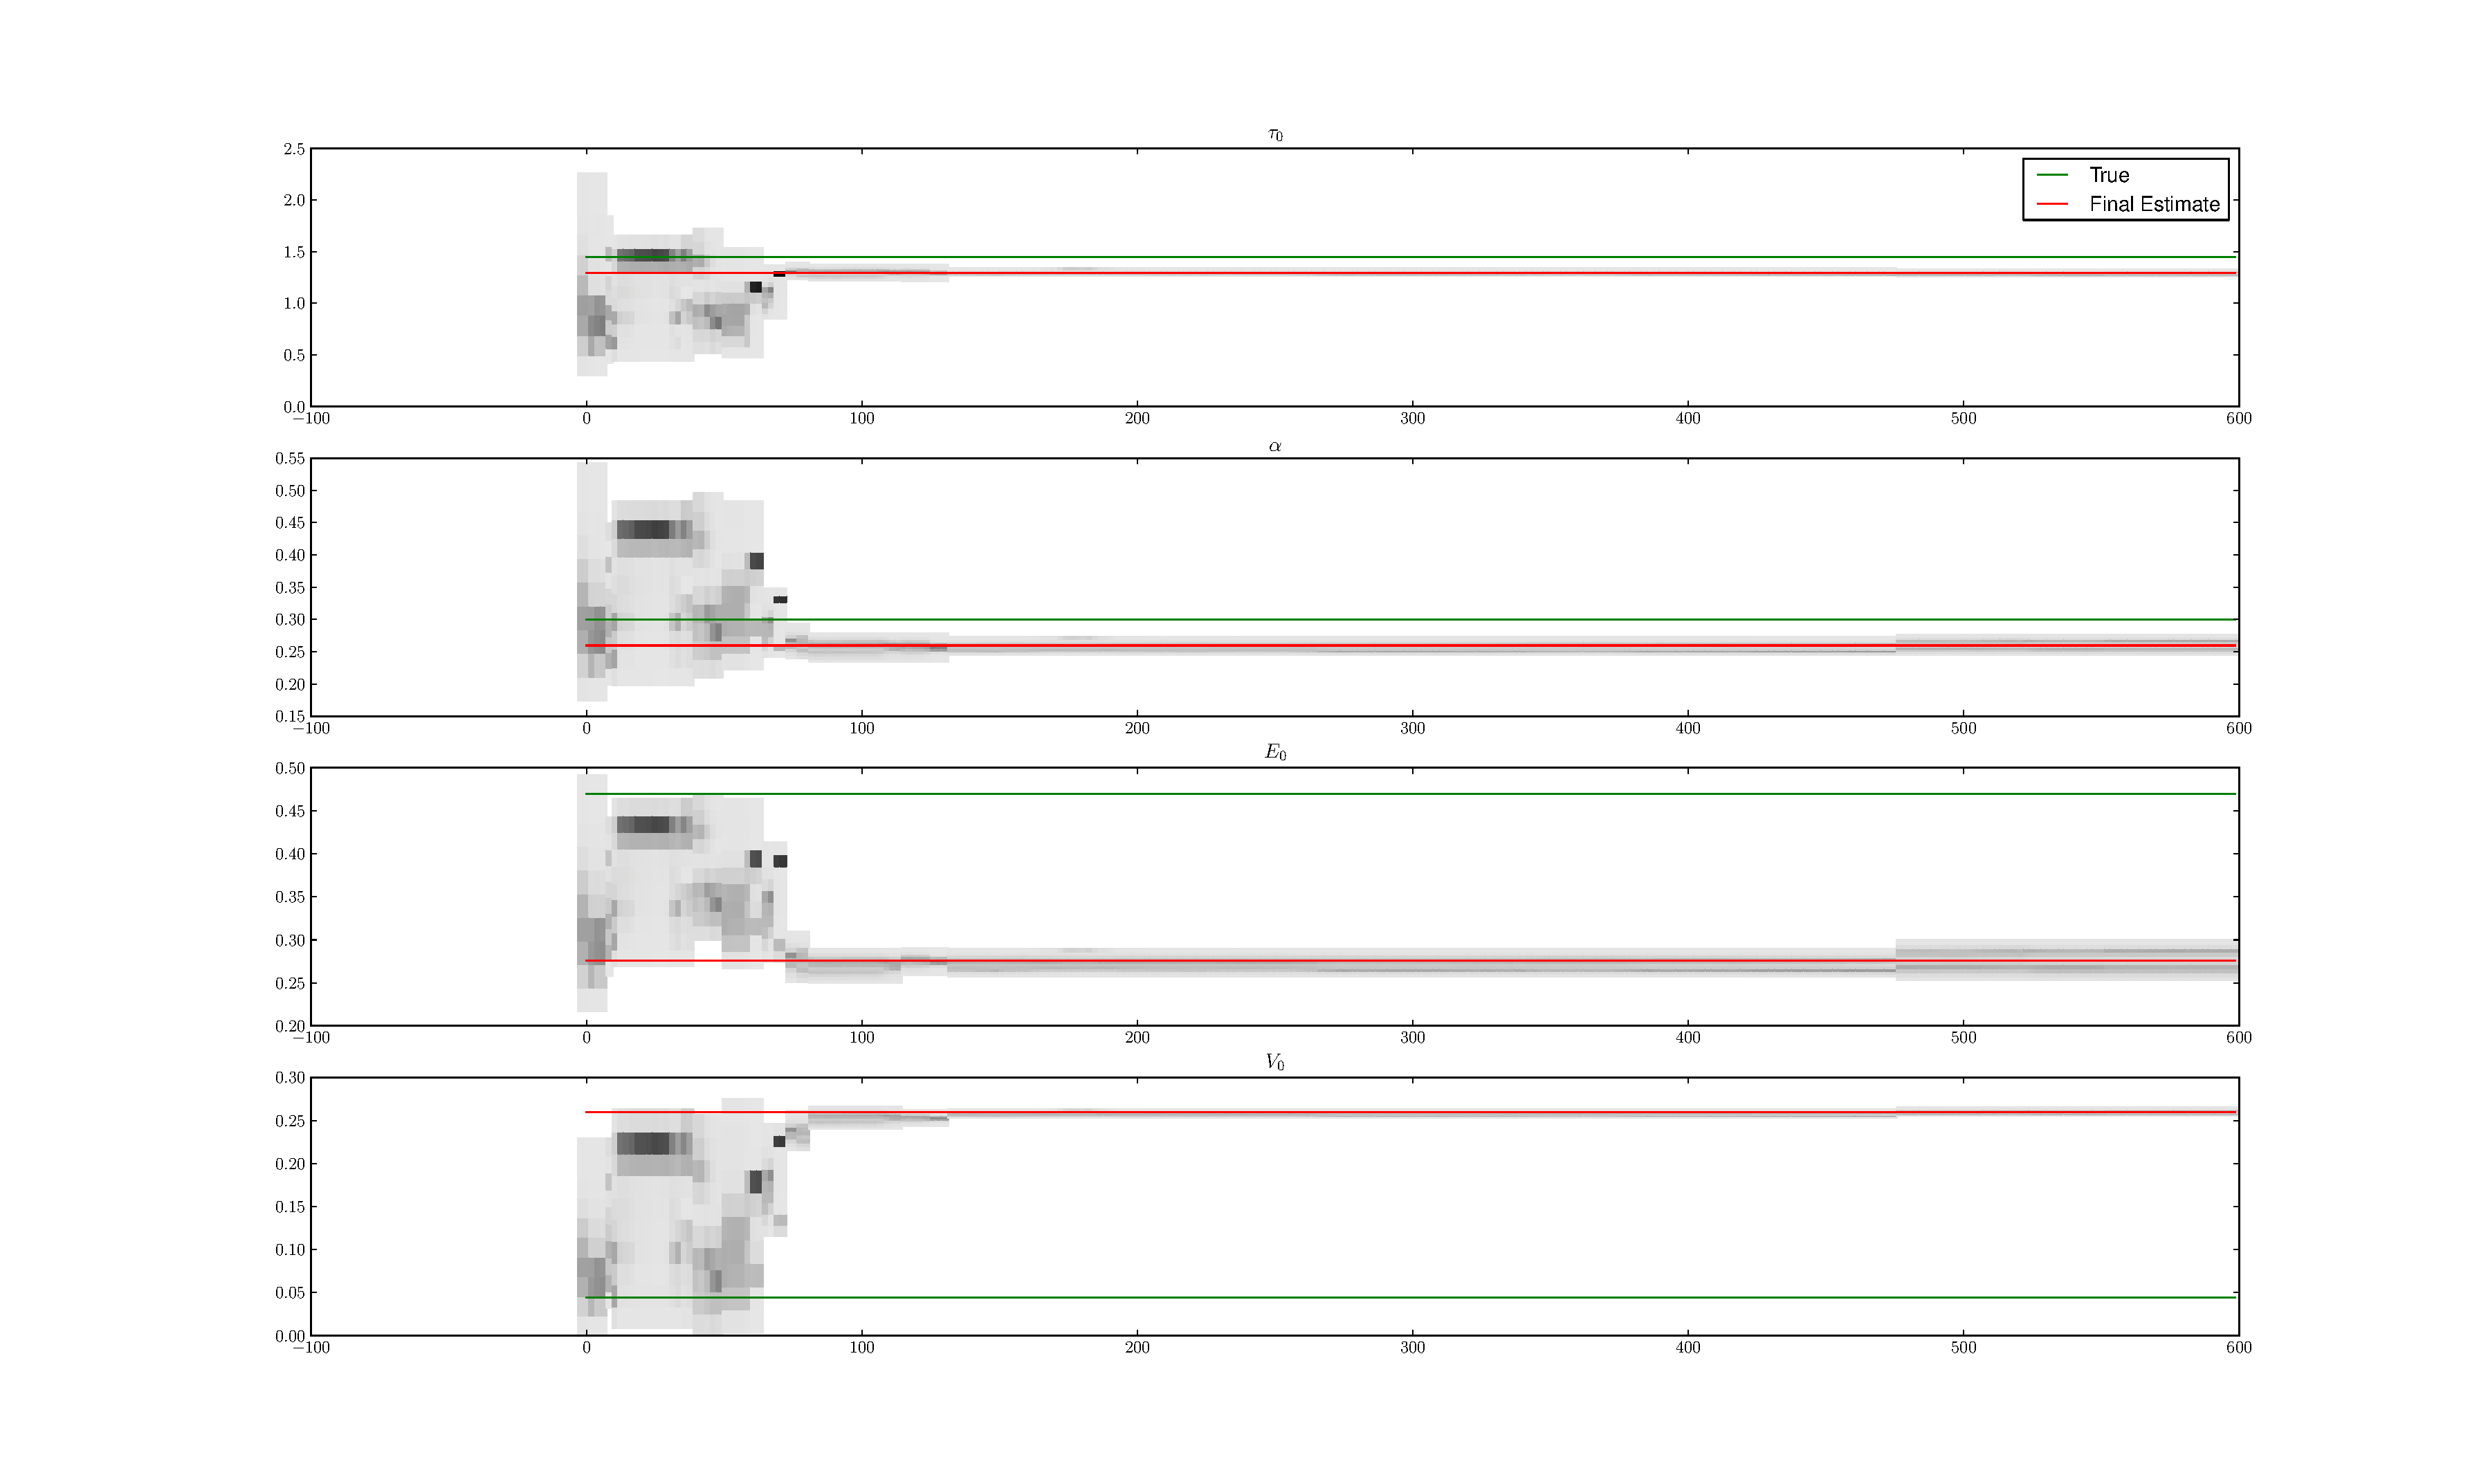
\includegraphics[trim=7cm 3cm 7cm 4cm, width=15cm]{images/highnoise_run5_1}}\\
\end{figure}
\begin{figure}[H]
\subfigure[$\tau_s$, $\tau_f$, $\epsilon$, $V$] 
{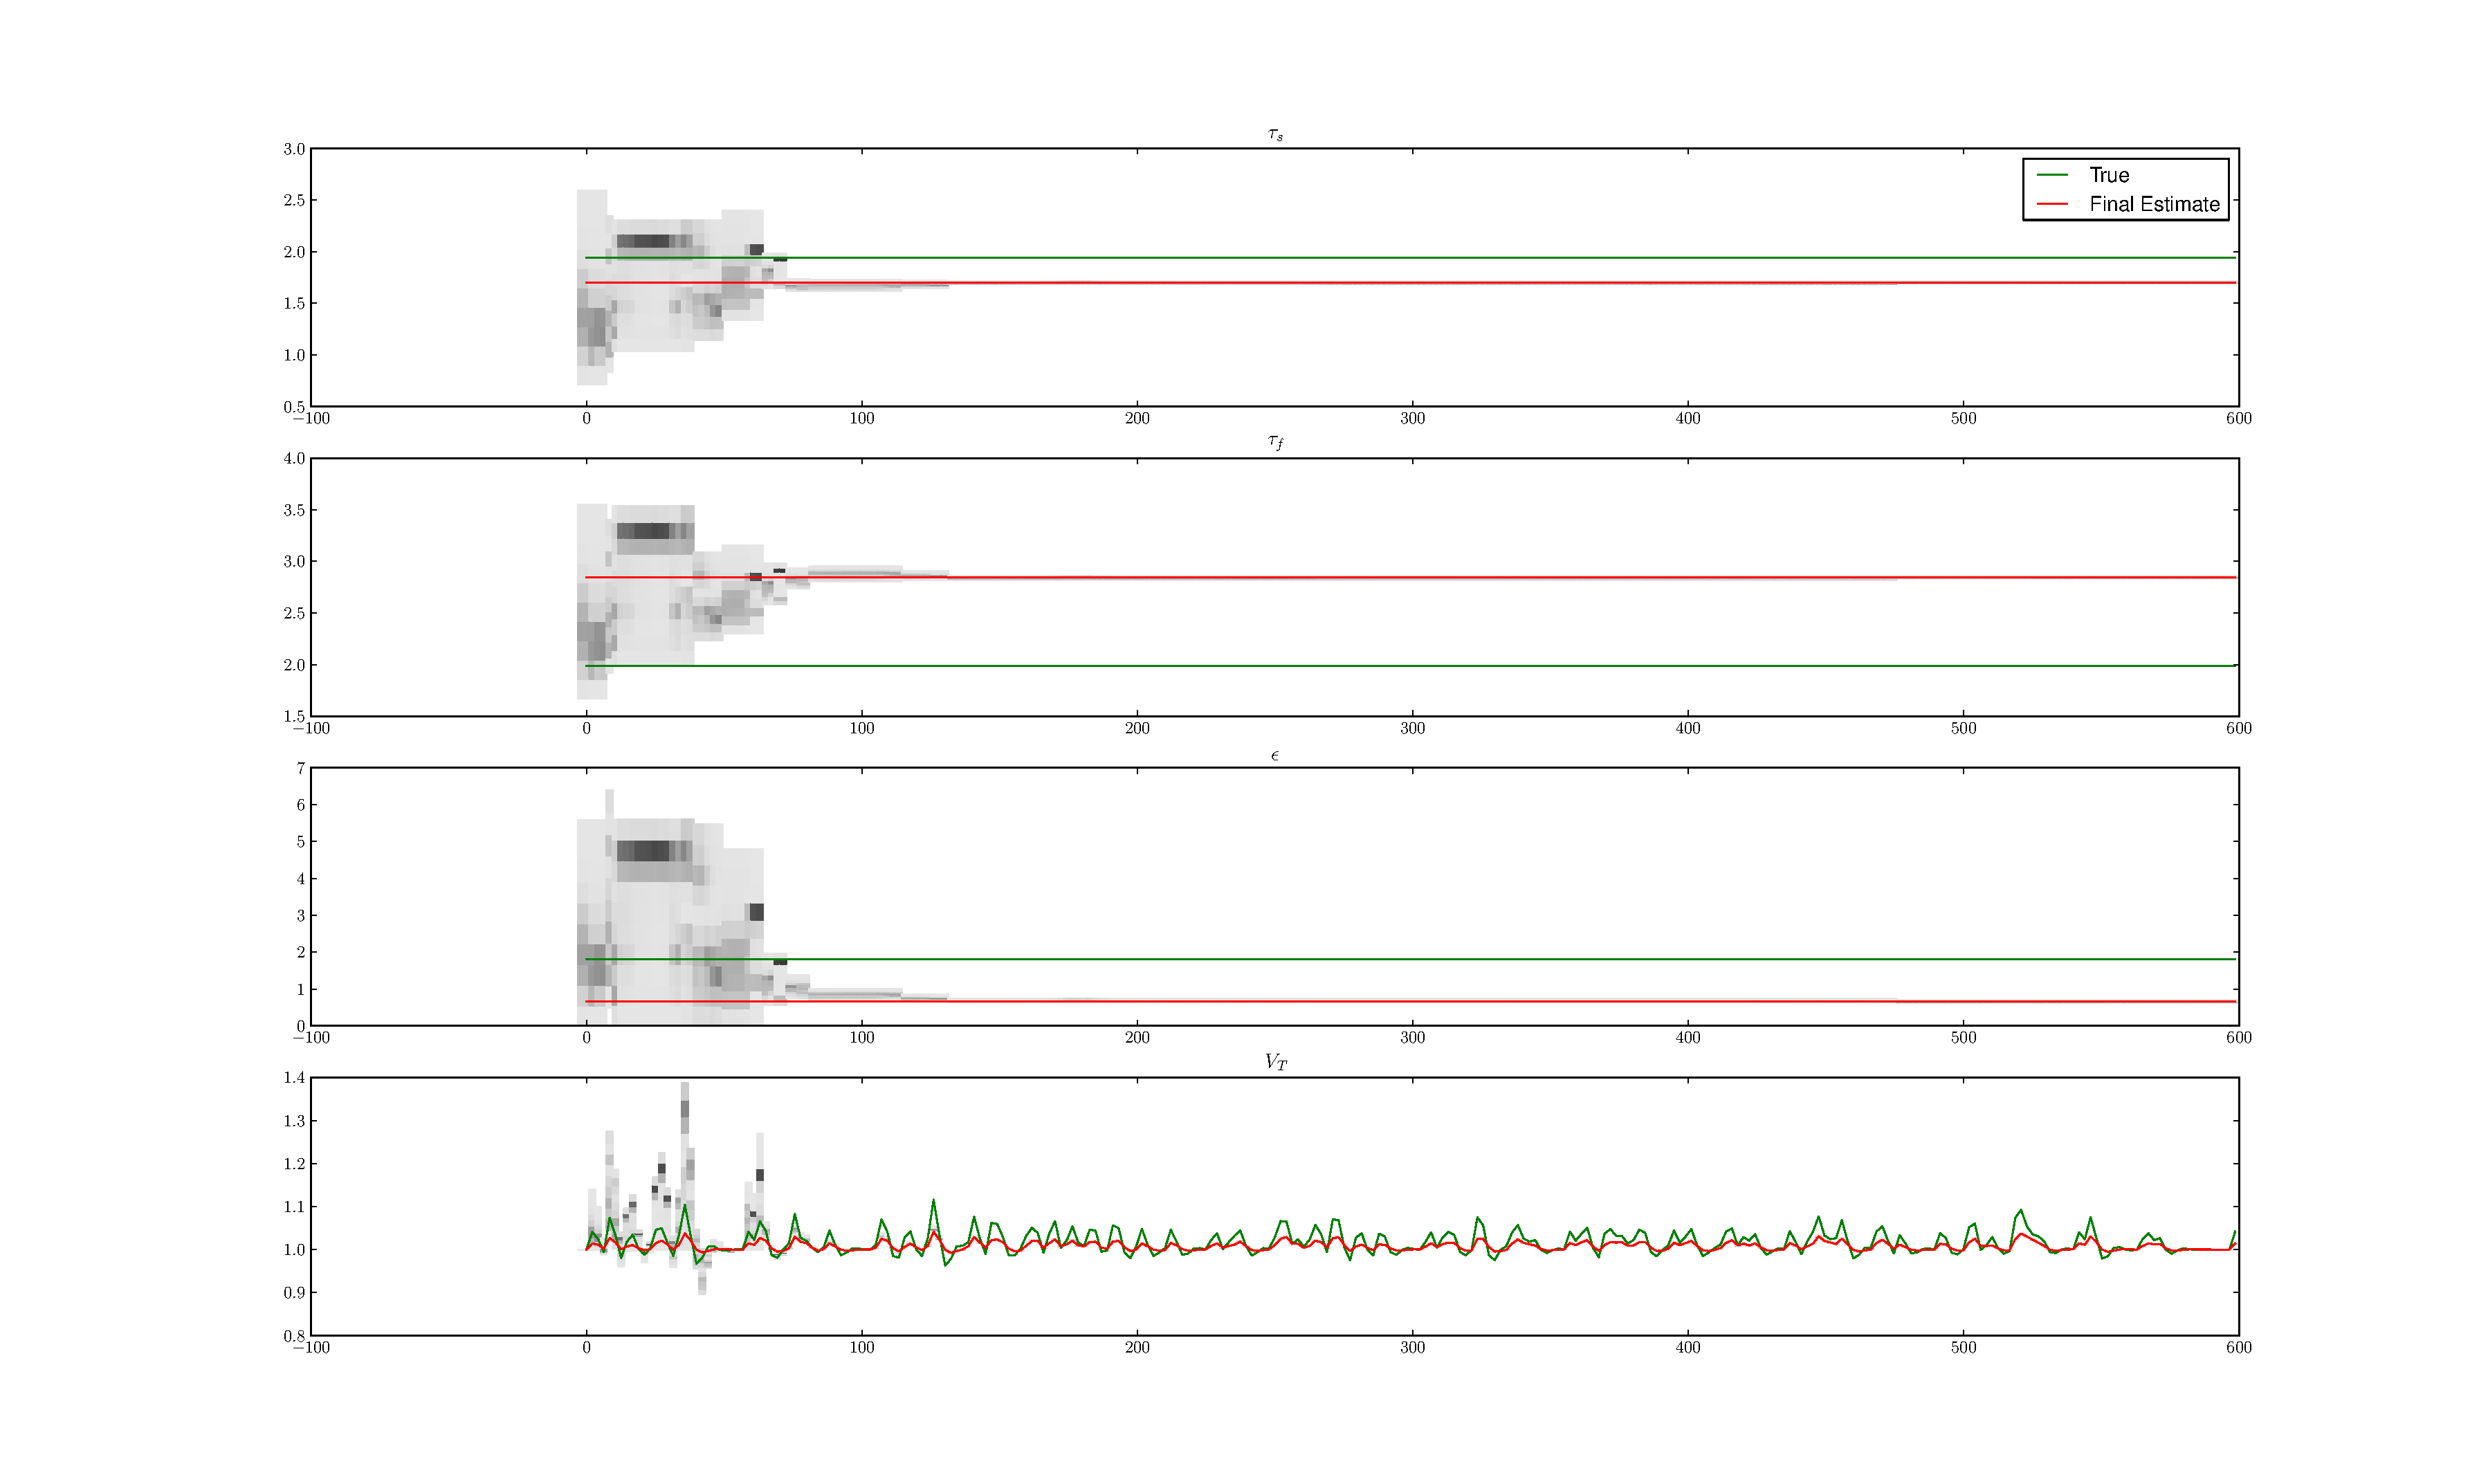
\includegraphics[trim=7cm 3cm 7cm 1cm, width=15cm]{images/highnoise_run5_2}}\\
\end{figure}
\begin{figure}[H]
\subfigure[$Q$, $S$, $F$, $BOLD$ ]
{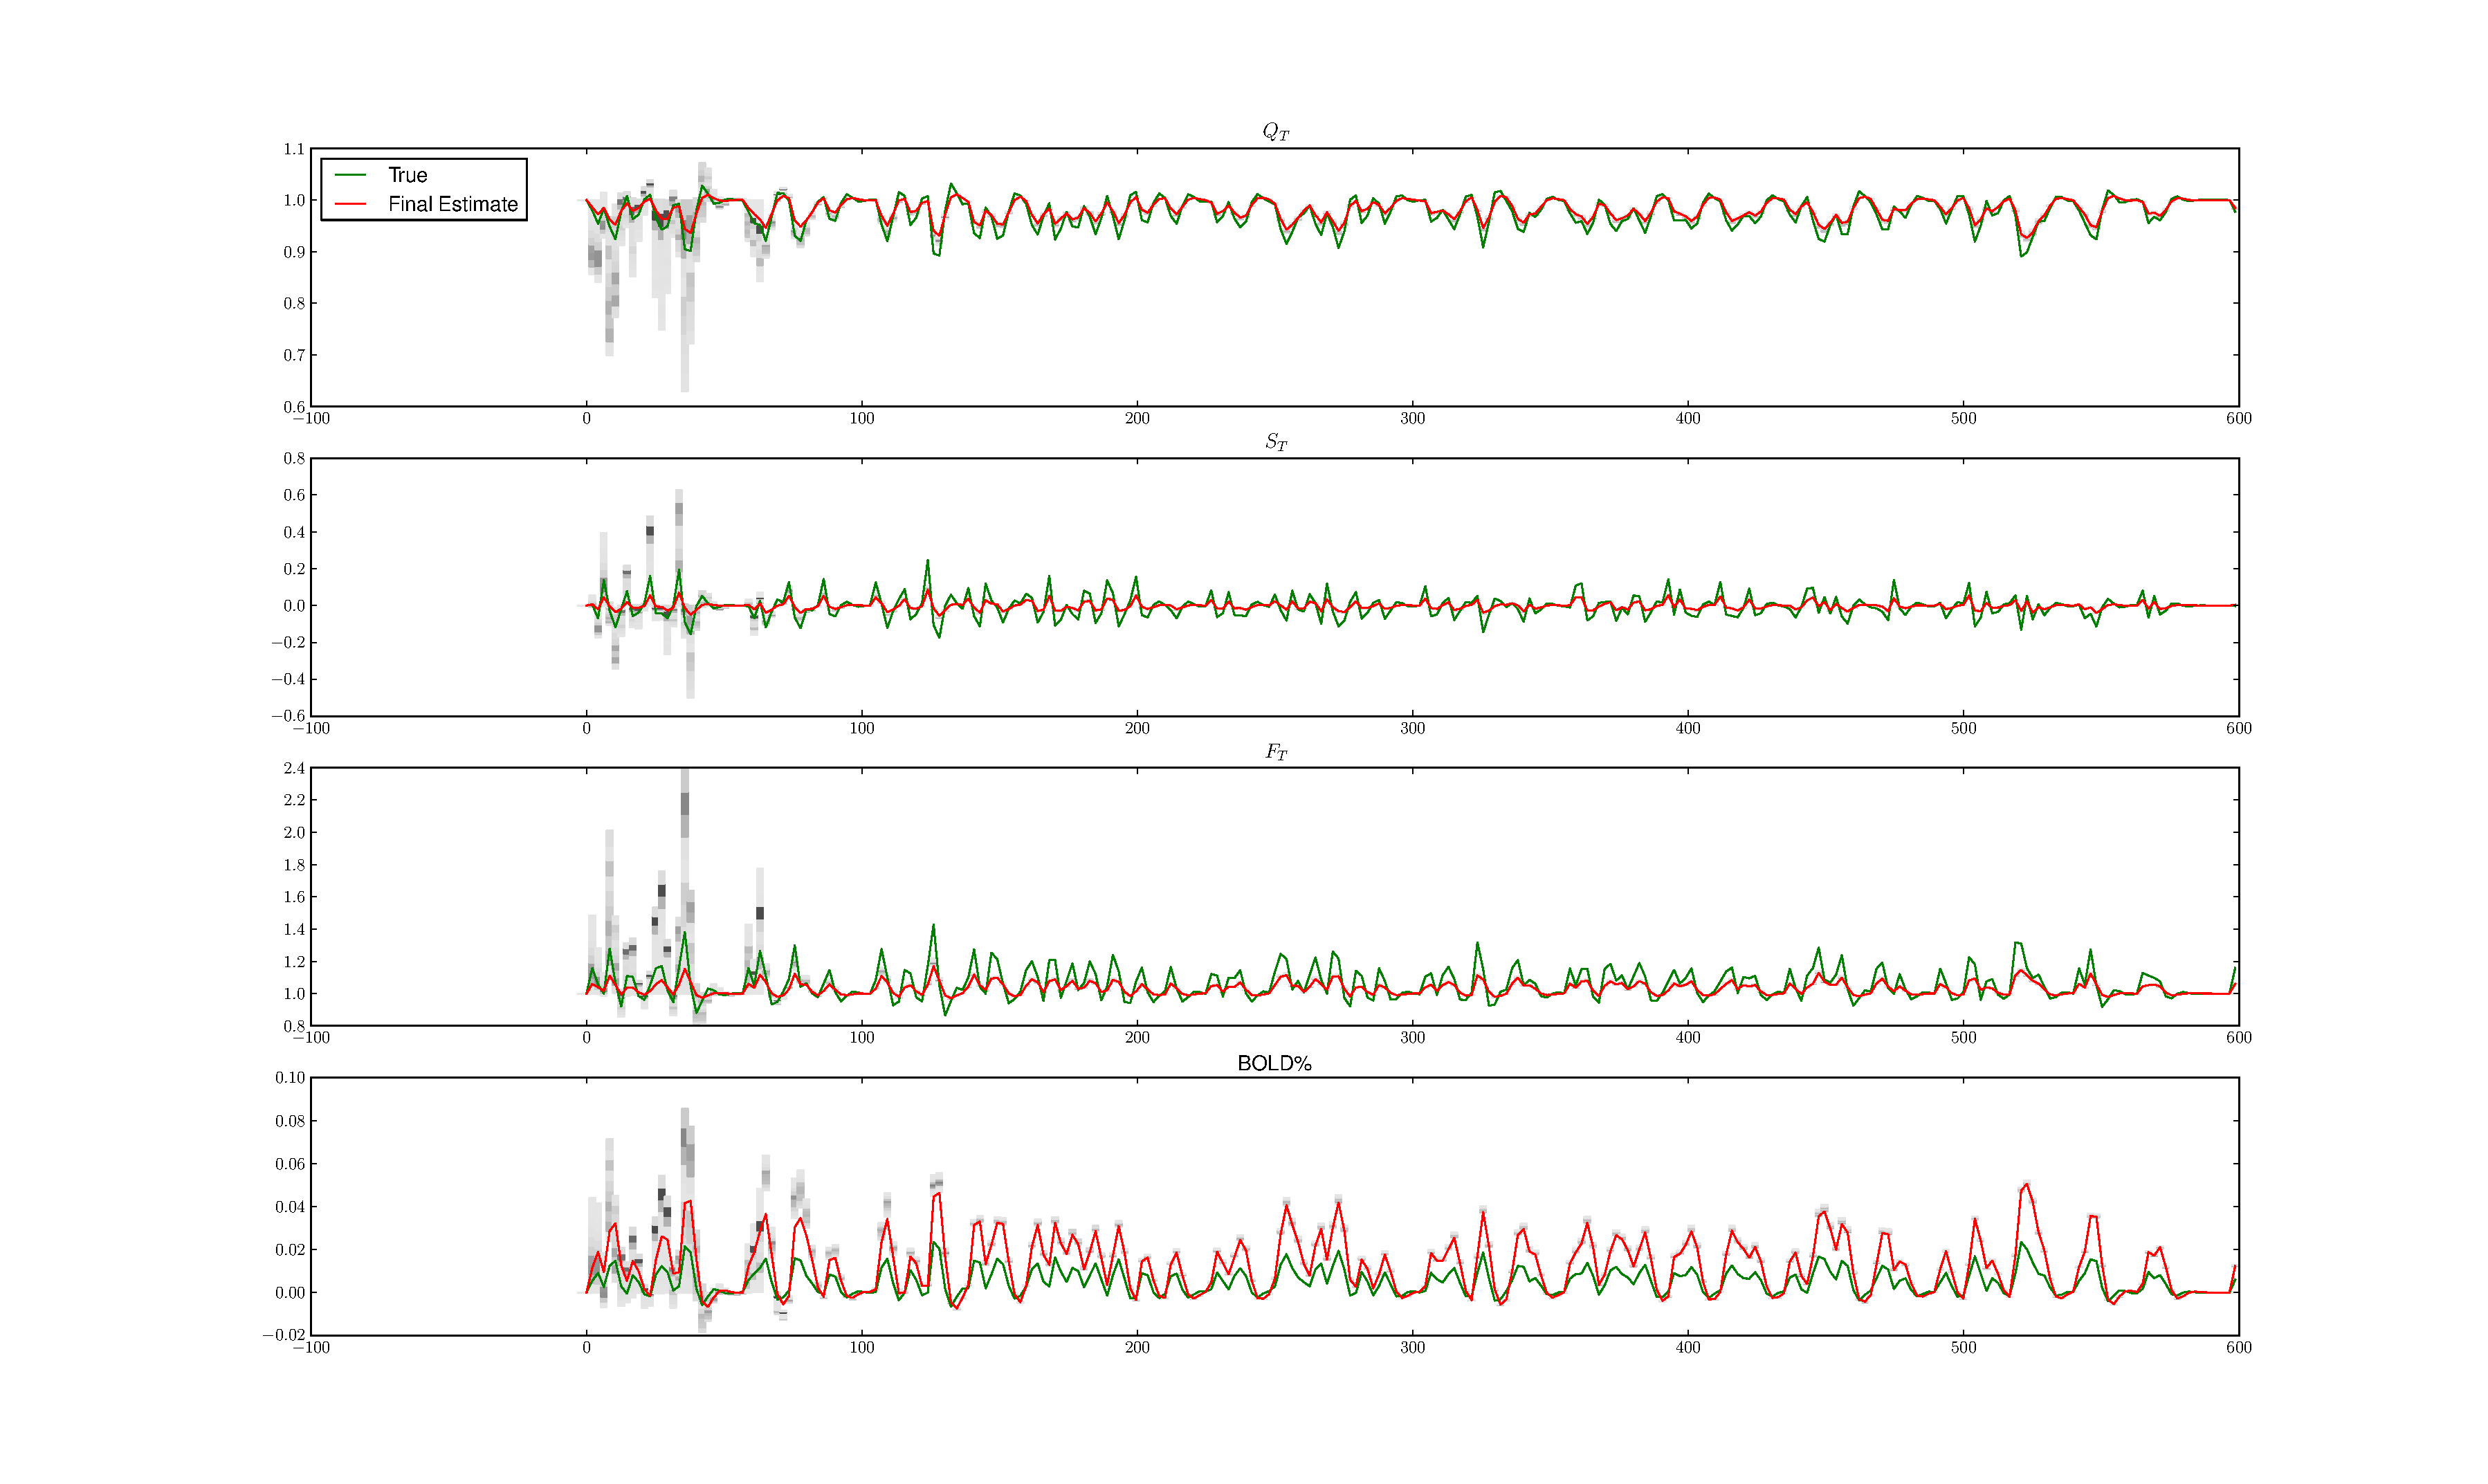
\includegraphics[trim=7cm 3cm 7cm 2cm, width=15cm]{images/highnoise_run5_3}}
\label{fig:ConvergenceRuns1}
\caption{Converging histogram for parameters during run 2, as in \autoref{fig:NoiseComparisonJustTwo}.}
\end{figure}

There are a number of interesting convergence properties of the
particle filter when more noise is present, as both \autoref{fig:ConvergenceRuns1} and
\autoref{fig:ConvergenceRuns2} show. Obviously the particle filter seems to converge
significantly faster, as points tend to be further out on the weighting function. This
also causes significantly more resampling which is the explanation for the seeming
jumps in resolution that occur from time to time. 

\begin{figure}[H]
\subfigure[$\tau_0$, $\alpha$, $E_0$, $V_0$]
{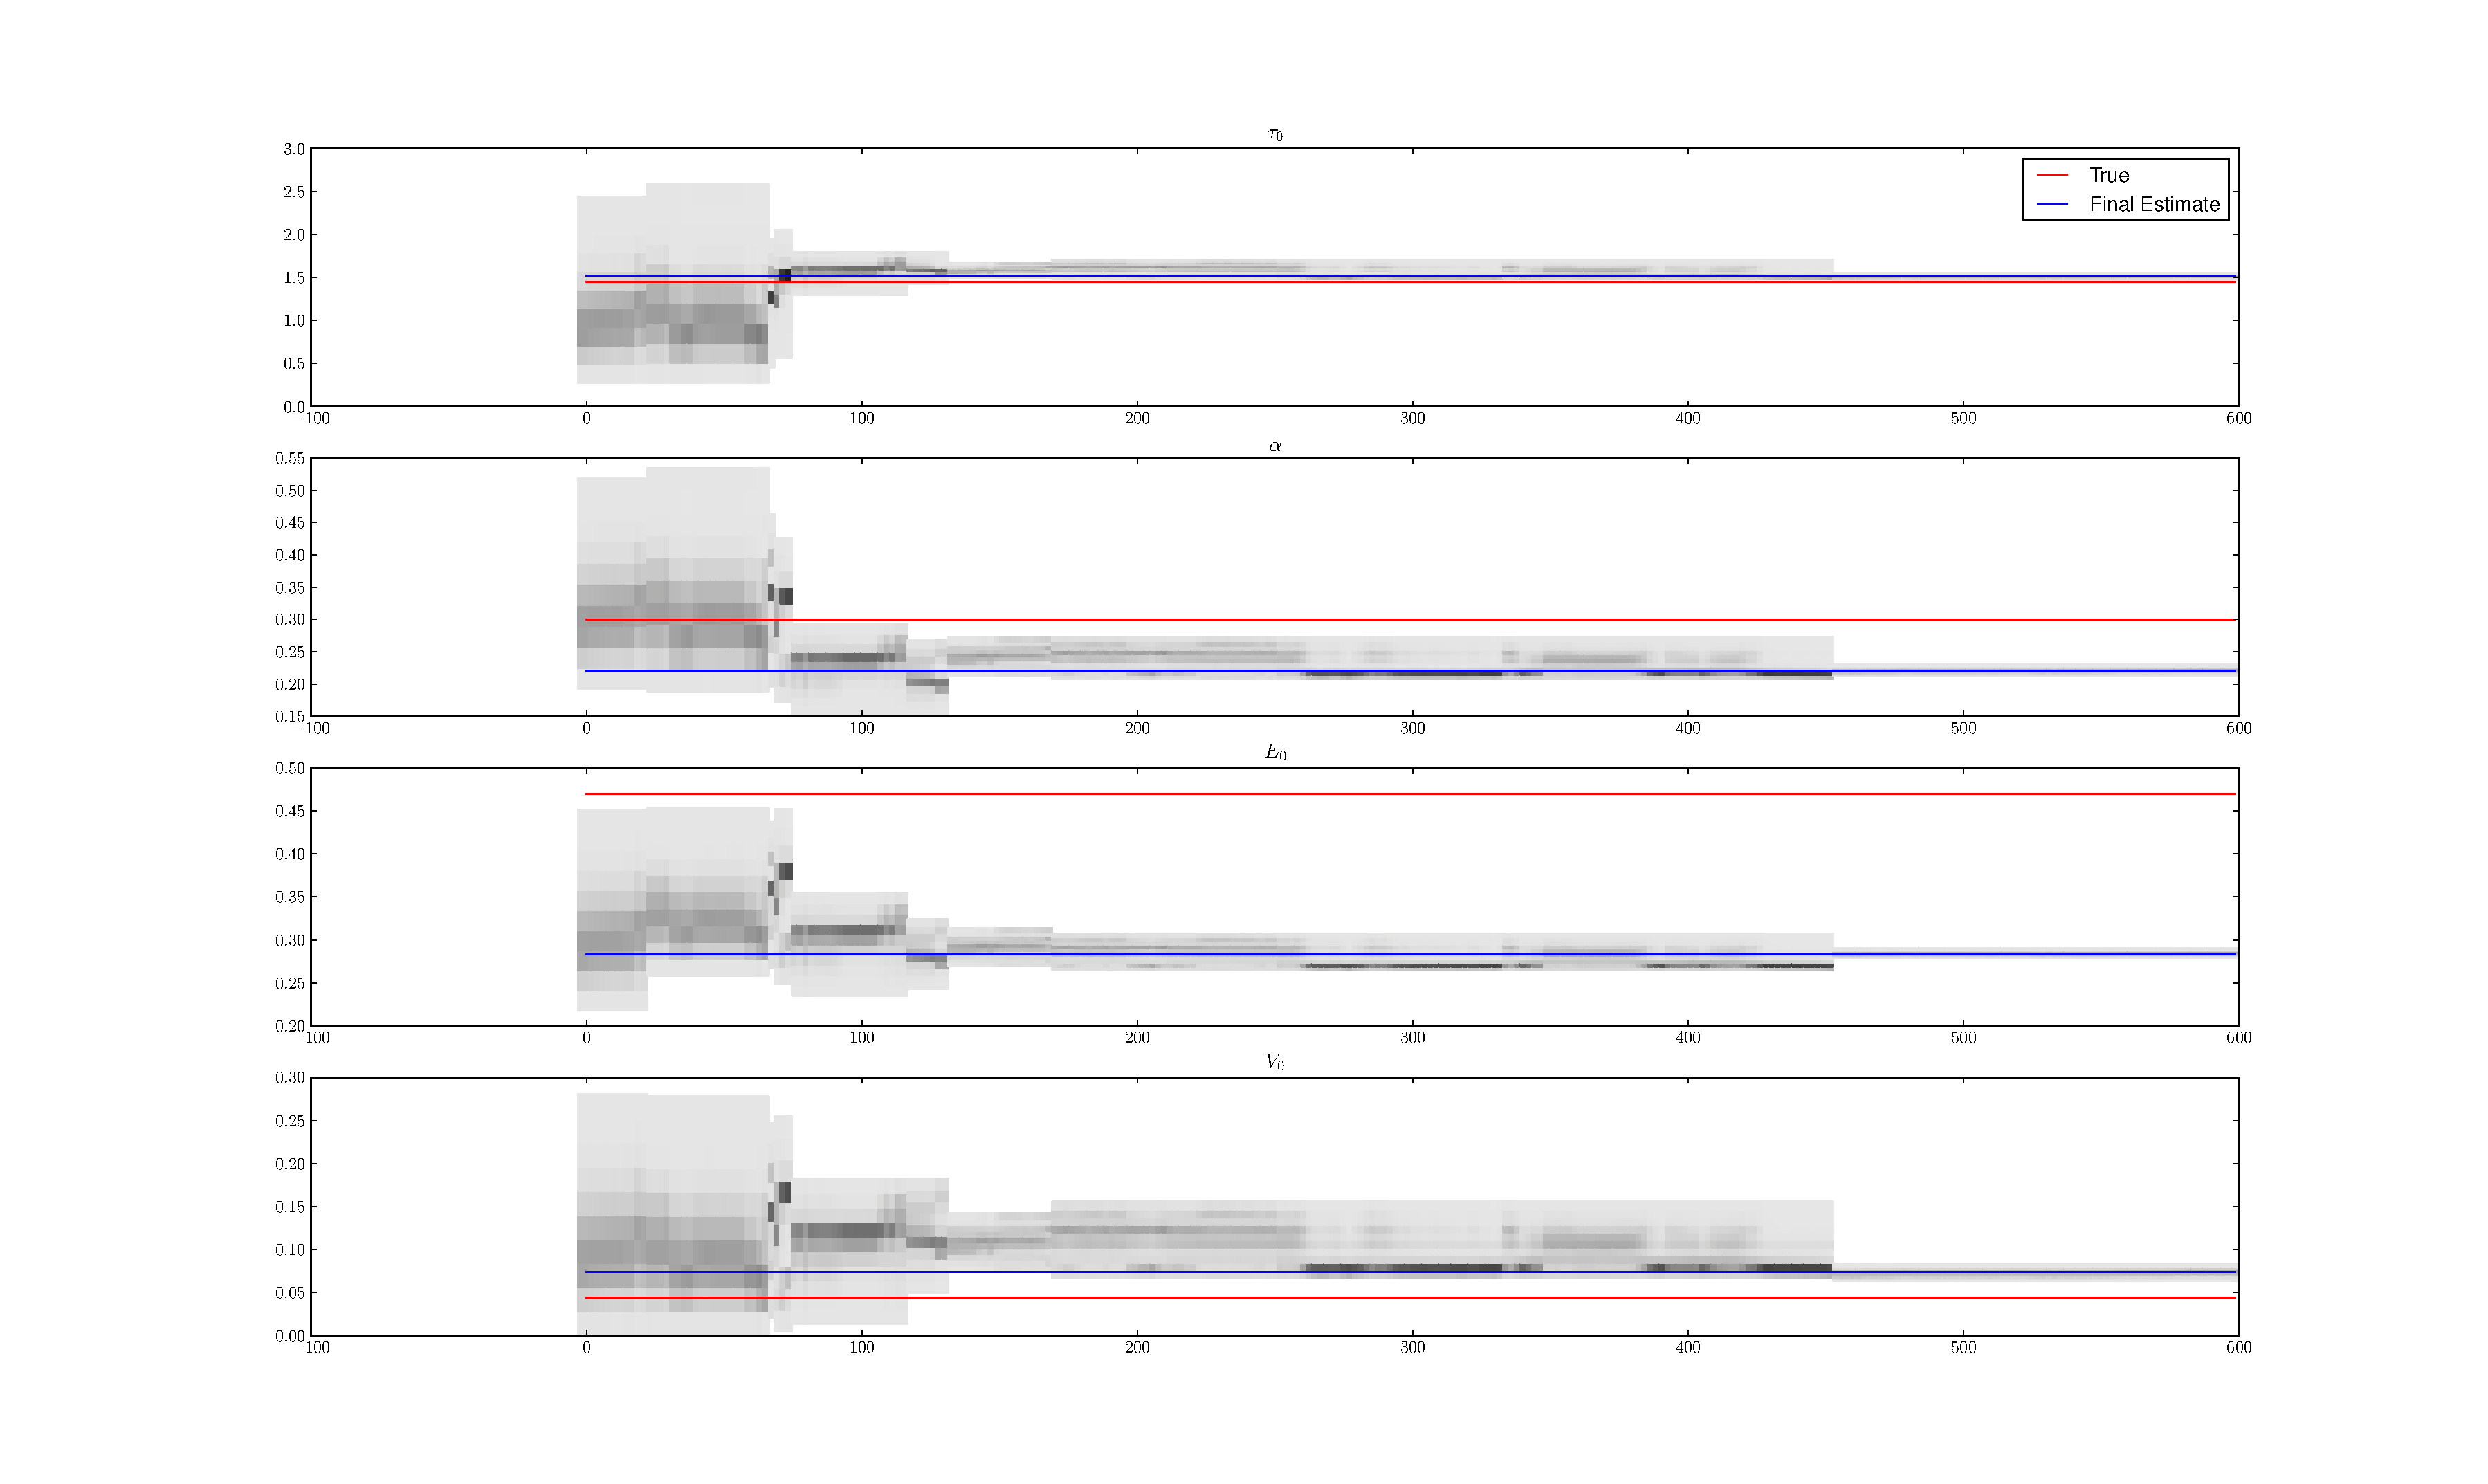
\includegraphics[trim=7cm 3cm 7cm 4cm, width=15cm]{images/highnoise_run6_1}}\\
\end{figure}
\begin{figure}[H]
\subfigure[$\tau_s$, $\tau_f$, $\epsilon$, $V$] 
{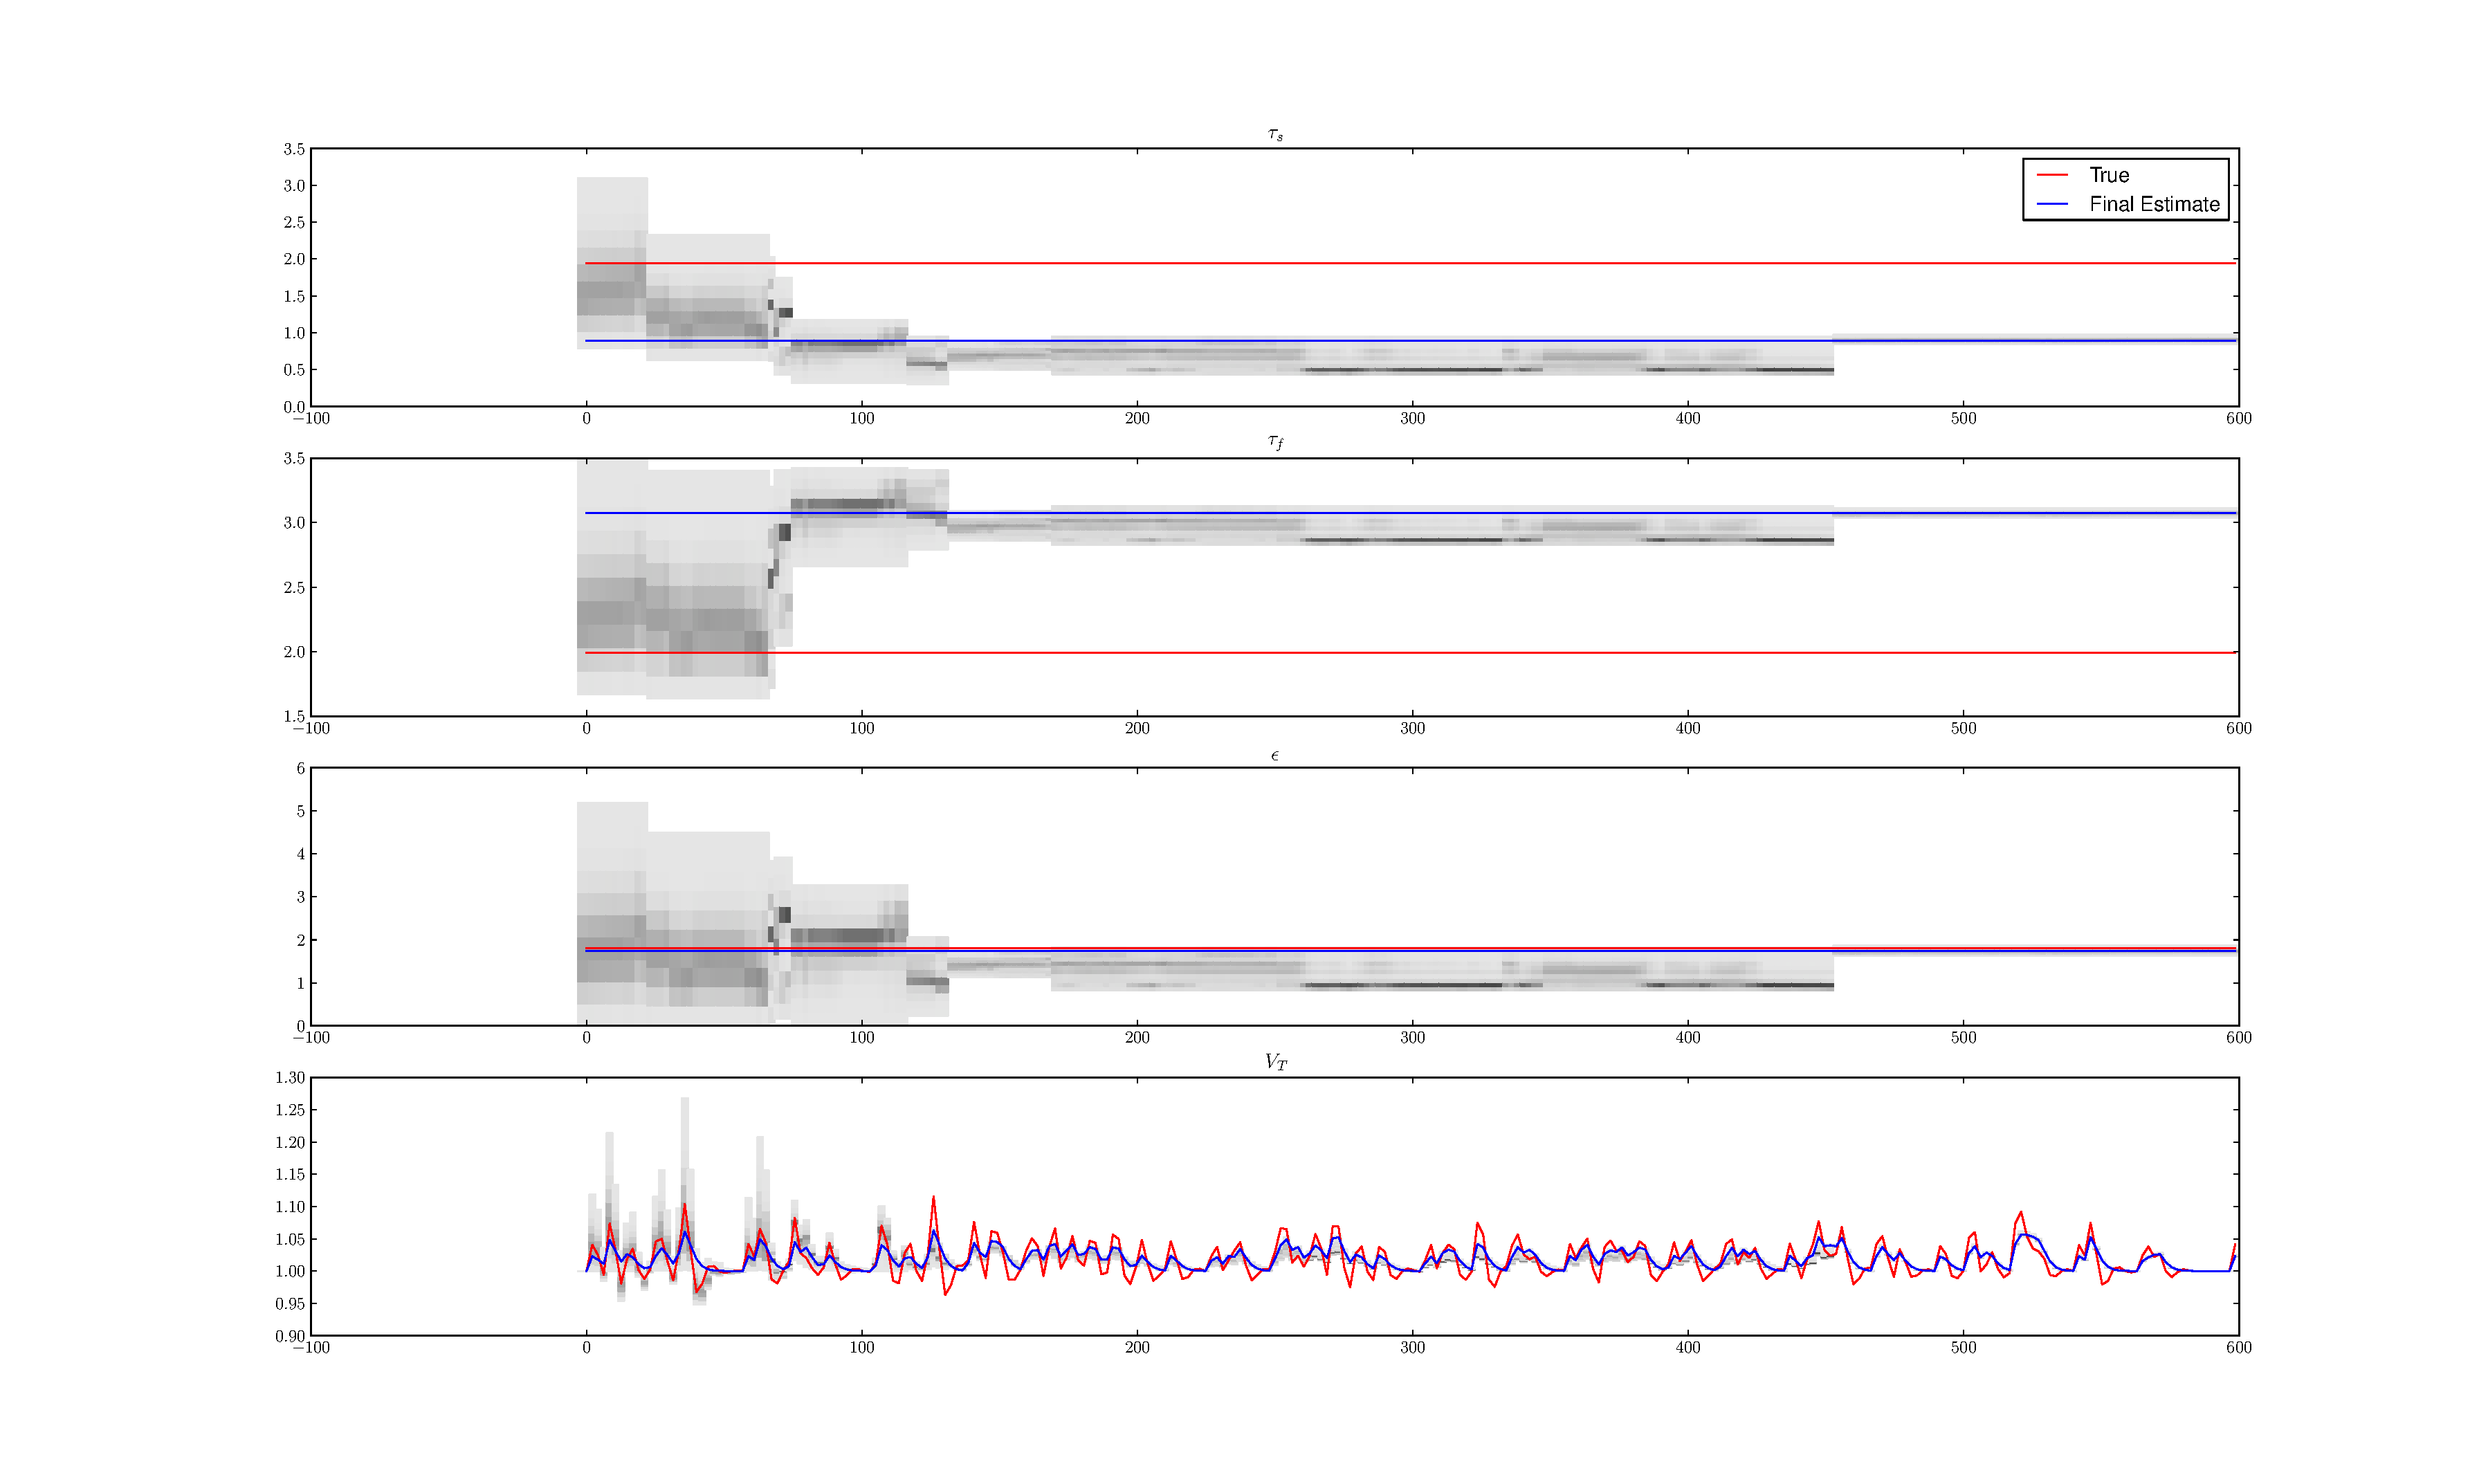
\includegraphics[trim=7cm 3cm 7cm 1cm, width=15cm]{images/highnoise_run6_2}}\\
\end{figure}
\begin{figure}[H]
\subfigure[$Q$, $S$, $F$, $BOLD$ ]
{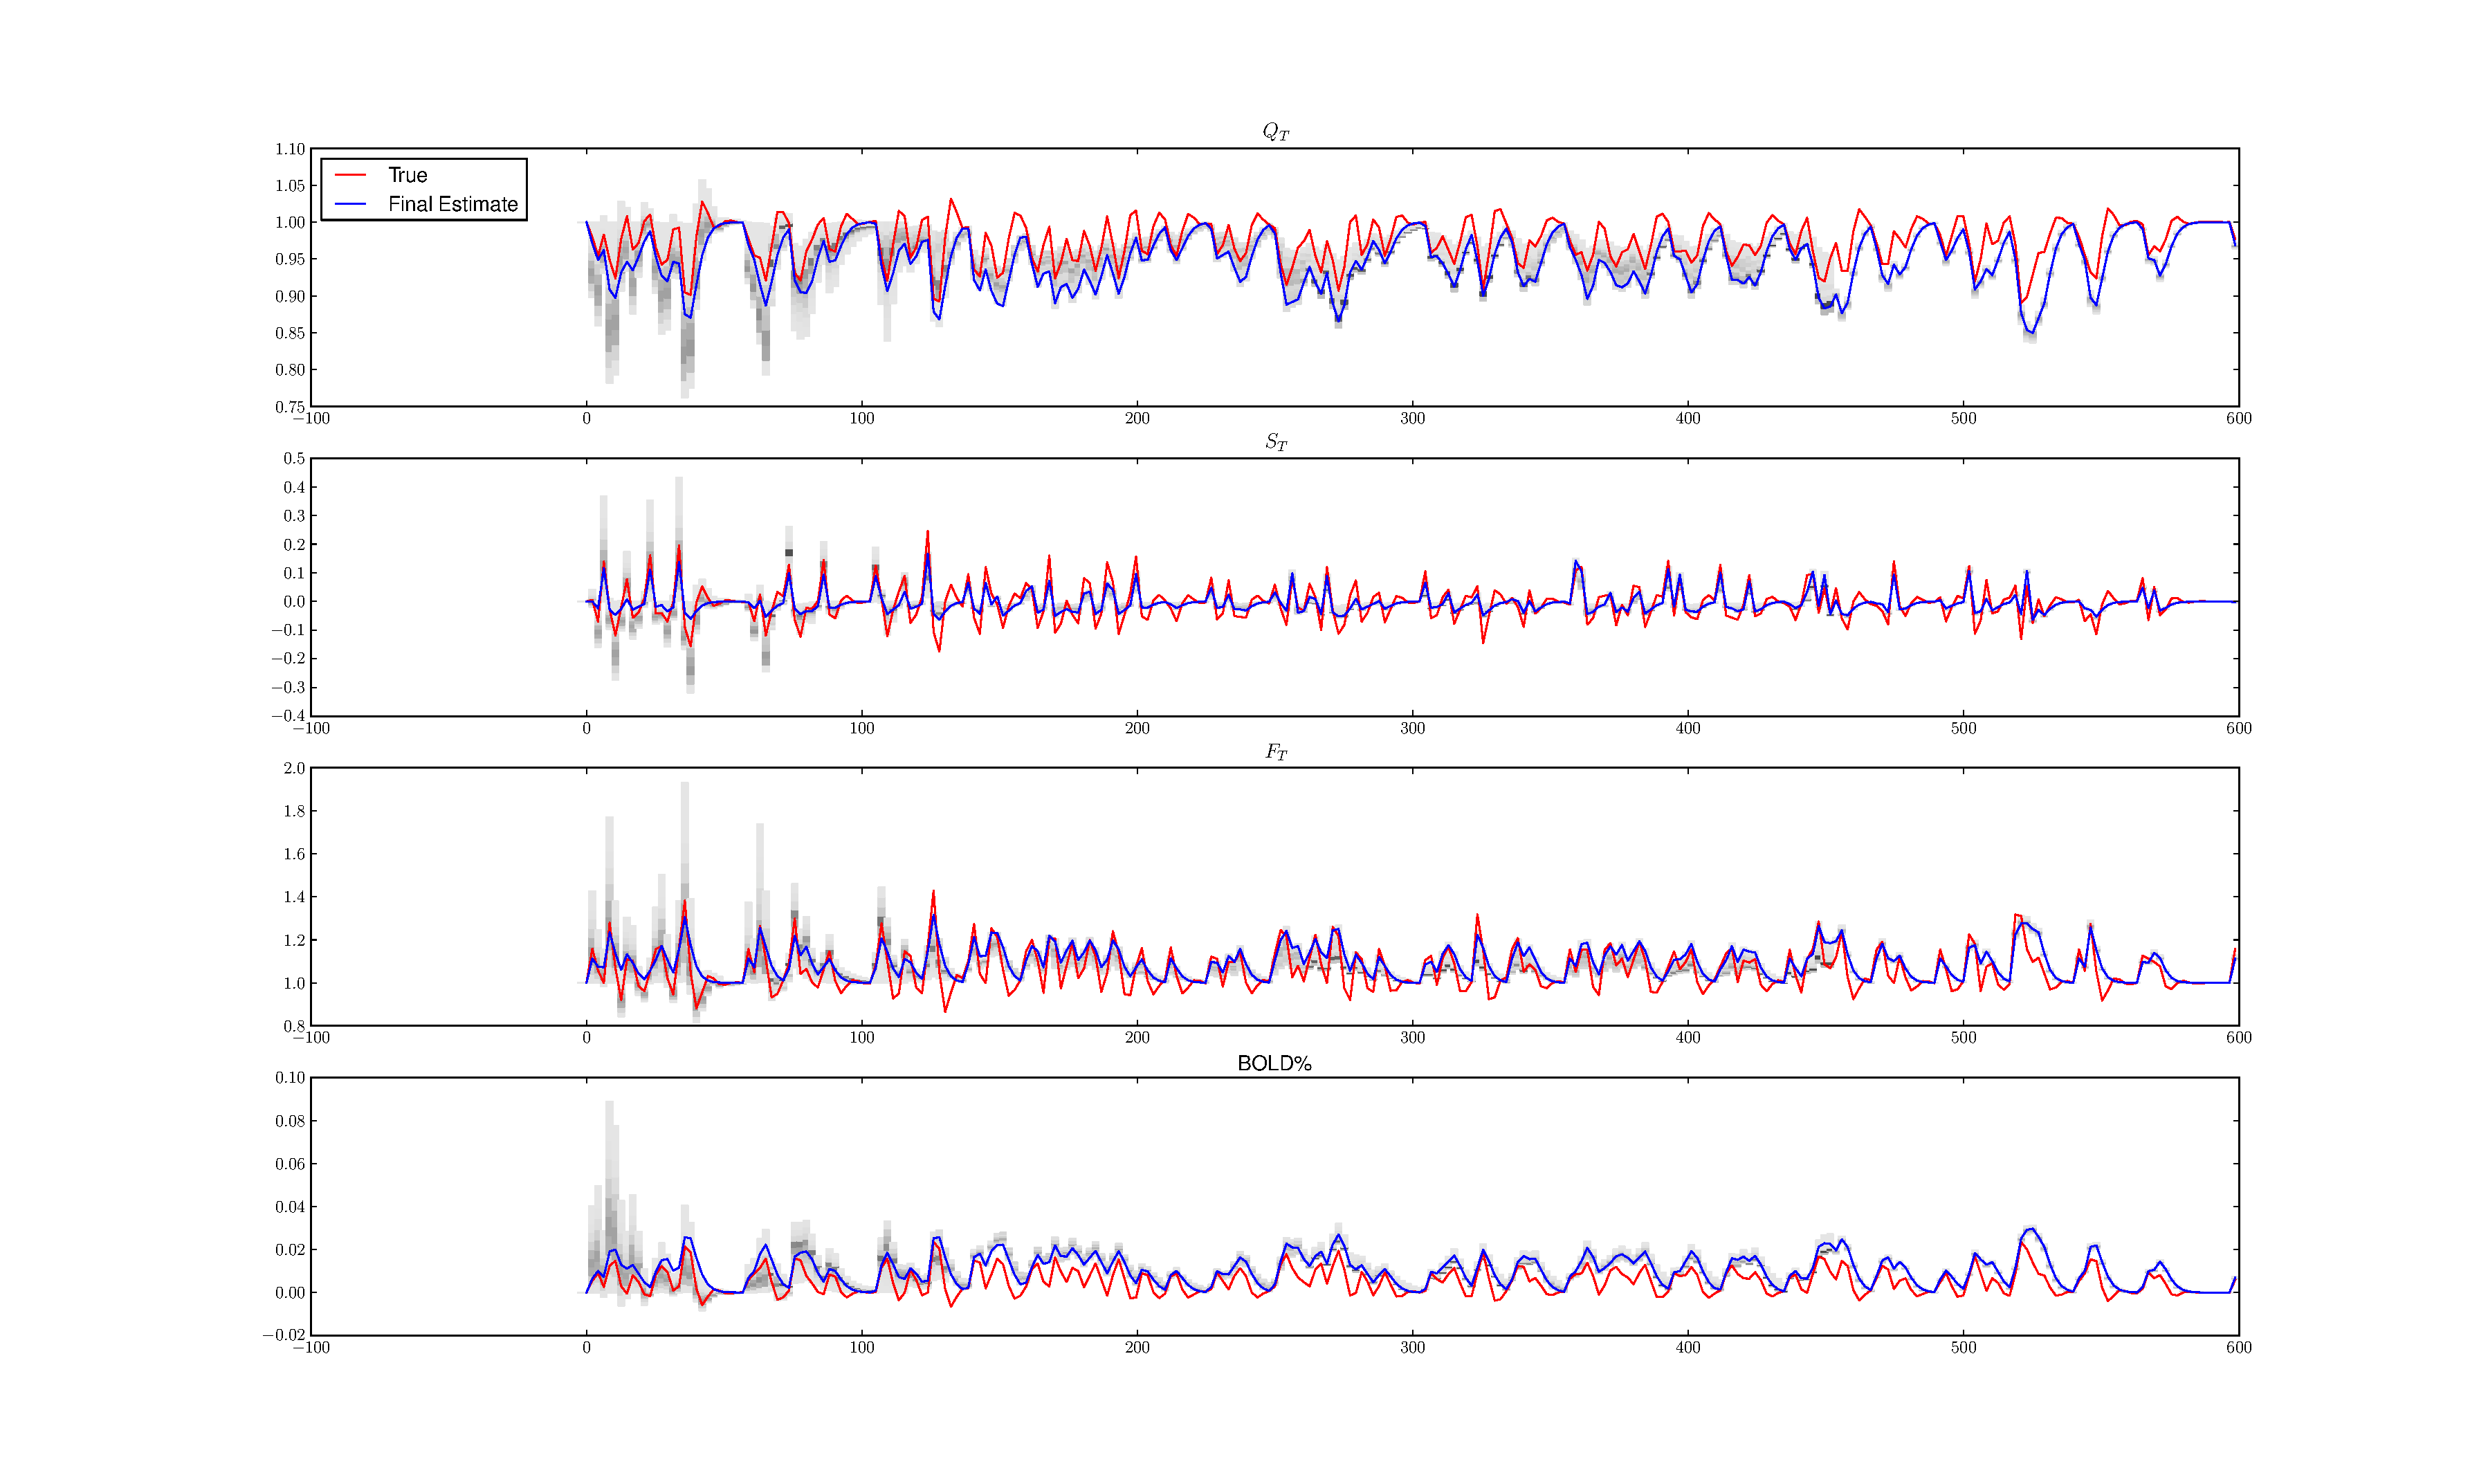
\includegraphics[trim=7cm 3cm 7cm 2cm, width=15cm]{images/highnoise_run6_3}}
\label{fig:ConvergenceRuns2}
\caption{Converging histogram for parameters during run 2, as in \autoref{fig:NoiseComparisonJustTwo}.}
\end{figure}

The parameters arrived at for all ten filter runs are shown in \autoref{tab:HighNoiseResults}.

\begin{table}[t]
\centering
\begin{tabular}{|c | c | c | c | c | c | c | c | c | c |}
\hline 
$\tau_0$ & $\alpha$ & $E_0$    & $V_0$    & $\tau_s$ & $\tau_f$ & $\epsilon$  & $ \sum \tau $ & $\sqrt{MSE}$ (Res.) & $\sqrt{MSE}$\\
\hline 
\rowcolor[gray]{.8}
1.45 & .3 & .47 & .044 & 1.94 & 1.99 & 1.8  & 5.38 &  & \\
\hline 
\hline 
1.19002 & 0.23495 & 0.42228 & 0.128 & 1.01468 & 2.47795 & 1.11677 & 4.68265   &0.0140648  &0.01572919   \\
0.9721 & 0.21902 & 0.30505 & 0.061 & 0.57801 & 1.99596 & 3.46135 & 3.54608    &0.0137314  &0.01377685   \\
1.57947 & 0.14153 & 0.33798 & 0.1079 & 0.5843 & 2.12475 & 1.78343 & 4.28852   &0.01275372 &0.01577449   \\
1.10937 & 0.2374 & 0.53491 & 0.0351 & 1.21862 & 3.07365 & 2.35039 & 5.40164   &0.0167258  &0.0115433    \\
1.10712 & 0.27535 & 0.33651 & 0.03161 & 1.50567 & 2.65181 & 4.19099 & 5.2646  &0.01369793 &0.01221607   \\
0.58026 & 0.47931 & 0.41354 & 0.11894 & 0.97563 & 3.69018 & 1.00084 & 5.24607 &0.01149511 &0.01315637   \\
\rowcolor[rgb]{.9,.5,.5}
1.29515 & 0.25957 & 0.27559 & 0.25952 & 1.70265 & 2.8458 & 0.66172 & 5.84361  &0.01555035 &0.01789781   \\
\rowcolor[rgb]{.5,.5,.9}
1.5185 & 0.21987 & 0.28348 & 0.07417 & 0.88822 & 3.07706 & 1.73929 & 5.48378  &0.01205351 &0.01246202   \\
0.68736 & 0.3283 & 0.39786 & 0.15614 & 1.07781 & 3.1158 & 0.66432 & 4.88097   &0.01510364 &0.01257713   \\
1.01703 & 0.28497 & 0.34741 & 0.05672 & 1.58774 & 2.65157 & 2.28519 & 5.25634 &0.012493   &0.01343459   \\
0.99247 & 0.29795 & 0.32207 & 0.20943 & 0.42757 & 2.21081 & 1.01674 & 3.63085 &0.01216522 &0.01505545   \\
\hline                                                                          
1.09535 & 0.27075 & 0.36152 & 0.11259 & 1.05099 & 2.71958 & 1.84282 & 4.86592 &0.01362132  &0.01396575\\
\hline 
\end{tabular}
\caption{Estimated Parameters on 10 different runs with high noise. First row is the true parameters.
Note also that the blue row is Run 1 and the red row is Run 2, as used named this section}
\label{tab:HighNoiseResults} 
\end{table}

a series of tests to determine the convergence rate of the particle filter, the number
of particles that were required, how weighting functions compared, how different de-trending
methods compared with each other and, finally the variance of the result. By running the exact
time-series with different noise realizations, it was possible to determine the model variance.
As the reader may know, the error of an estimator may be calculated as:
\begin{equation}
MSE(\Theta) = Var(\Theta) + Bias(\Theta)^2
\end{equation}
The variance is an expression of how much the result would change for different noise realizations,
whereas the bias is an expression of how well the model matches the true underlying model. In
this case, because the same model is being used in the particle filter and underlying simulation,
the bias is actually zero. Obviously when this is calculated using \emph{real} data with an unknown
underlying state space equation, there will be some amount of bias error, but assuming that the
noise is similar to the noise used in these tests, the model variance will actually be about the
same. Thus calculating the model variance is extremely helpful in calculating how well determined
our model is, and how consistent it will be for real data. A single timeseries, as opposed to the
thousands present in a real image, makes it easier to 
compare the output with the ground truth, with various parameters. 

Second I used a modified version of the FSL tool 
POSSUM to generate an entire FMRI image from a parameter map. The parameter map was generated
by taking an existing activation map and assigning discrete parameter sets to each region.
The result was a four dimensional (length x width
x height x parameter) image with spatially varying parameters. Possum was then modified
to take a parameter map and generate activation levels depending on the parameters at that
point. The patch for POSSUM will be made available. As an unfortunate side effect of 
not using Possums' original activation scale, I manually added 750 to the total level of
simulated Possum images. This is because the BOLD \% difference levels were in the range
of 50 - 100\% from the base, about 5 times as large as they should have been. Ultimately
this should not have an effect on the parameters (other than perhaps $\epsilon$ and $V_0$). 
For each time-series in the simulated FMRI image, the final \emph{static} parameters were saved
into a parameter map. This parameter map may then be compared to the map used to generate the 
simulated data; additionally a new simulation using the calculated parameters may also be 
generated to test the difference in activation levels between the real parameters and the
estimated ones. Since it is clear that the parameters are not fully orthogonal 
(\cite{Deneux2006}), its possible that two sets of parameters are functionally equivalent,
but have different parameters. This way, an absolute 
quantitative difference between the two parameter sets may be found.

\section{Real Data}
Finally, we also performed inference based on real FMRI data. The scanner we used...
%... more specifics...

Before performing tests on a full image, I tested the results of the particle filter
on regions deemed active and non-active by statistical parametric mapping. 
\section{Single-Voxel Simulation}
The results 

\section{Single-Voxel Analysis}
This section discusses the results when the particle filter was
applied on a single voxel. The parameters are the same as
those used later for entire image analysis; however, the results
are more in-depth. 

The run-time for a single voxel depends on the several factors. First, the
overall length of the signal being analyzed. For 1000 measurements it takes
about 10 to 15 minutes. On the other hand, in real circumstances the
length is only around 150 measurements. The number of  integration
can certainly make a large difference, however dropping below 1000 (.001 seconds)
is definitely not recommended. 

For a period I considered 1000 to be a
fine number; however when generating simulated data I found that every once
in a while 1000 was not enough. This is problematic in the actual particle
filter since, given the large number of simultaneous integrations taking 
place, its likely that a few particles will fail and be weighted at 0 because
of this problem. Additionally, because the typical case where a failure would
occur is at fast moving times/parameters the particles all tend to fail together.
The result is particle deprivation - no particles with non-zero weights remain.
The other possible outcome is that low time constant particles get pruned resulting
in excessively smoothed estimates for the time series'. Its possible that a
kind of stop-gap measure could be put into place; wherein particles that are
about to be set to NaN are integrated again with finer grained steps. However
many times the non-real results don't occur until several time steps after the 
numbers get strange. So for instance, the timestep was too long, allowing 
$f$ to go negative, resulting in extremely large values of $q$. There are many
different ways where this sort of event can occur, and unfortunately sometimes
there is no way to get back to before the state starting going out of control.

Another crucial factor for run time is how long before the first re-sampling 
occurs. Because the prior is represented initially with significantly more
particles, if the model fits very well, or for some reason the effective
number of particles stays high, resampling could take a long time to occur.
When this happens the particles filter can take a factor of 10 longer to run.
However, if the particle count isn't initially set high, there is a much larger
chance of particle deprivation occurring. Since there is no real way to know
how long it will take to resmaple the first time, there is little the 
algorithm can do to fix this (except perhaps forcing resampling after
some period of time). On the other end of the spectrum, if the time
series doesn't match the model at all, particle deprivation will occur extremely
quickly.  The upshot of this is that the particle filter is able to 
identify these sections very quickly, and thus not waste much time there.
The difficulty though, is the regions in between the perfect fit and the
awful fit. If particle deprivation does occur, did it occur randomly to an
activated region or did it occur inevitably because the region doesn't fit.
The reason for having so many initial particles is to give density to the
distribution to make false negatives more rare. Perhaps the correct method
is to still set the initial particles very high, but if for a long time no
resampling occurs, halve the standard deviation of the measurement error.
Thus, if the weighting function is not discriminating enough, force it 
to be more picky about the results. Of course this could lead to particle
deprivation as well if the standard deviation is brought down too quickly.
Of course, if a fat-tailed distribution is used for the weighting function,
or the standard deviation of a Gaussian weighting function is sufficiently large,
the particle filter will simply converge to meaningless values. The question
of whether 

\begin{figure}
\label{fig:badfit}
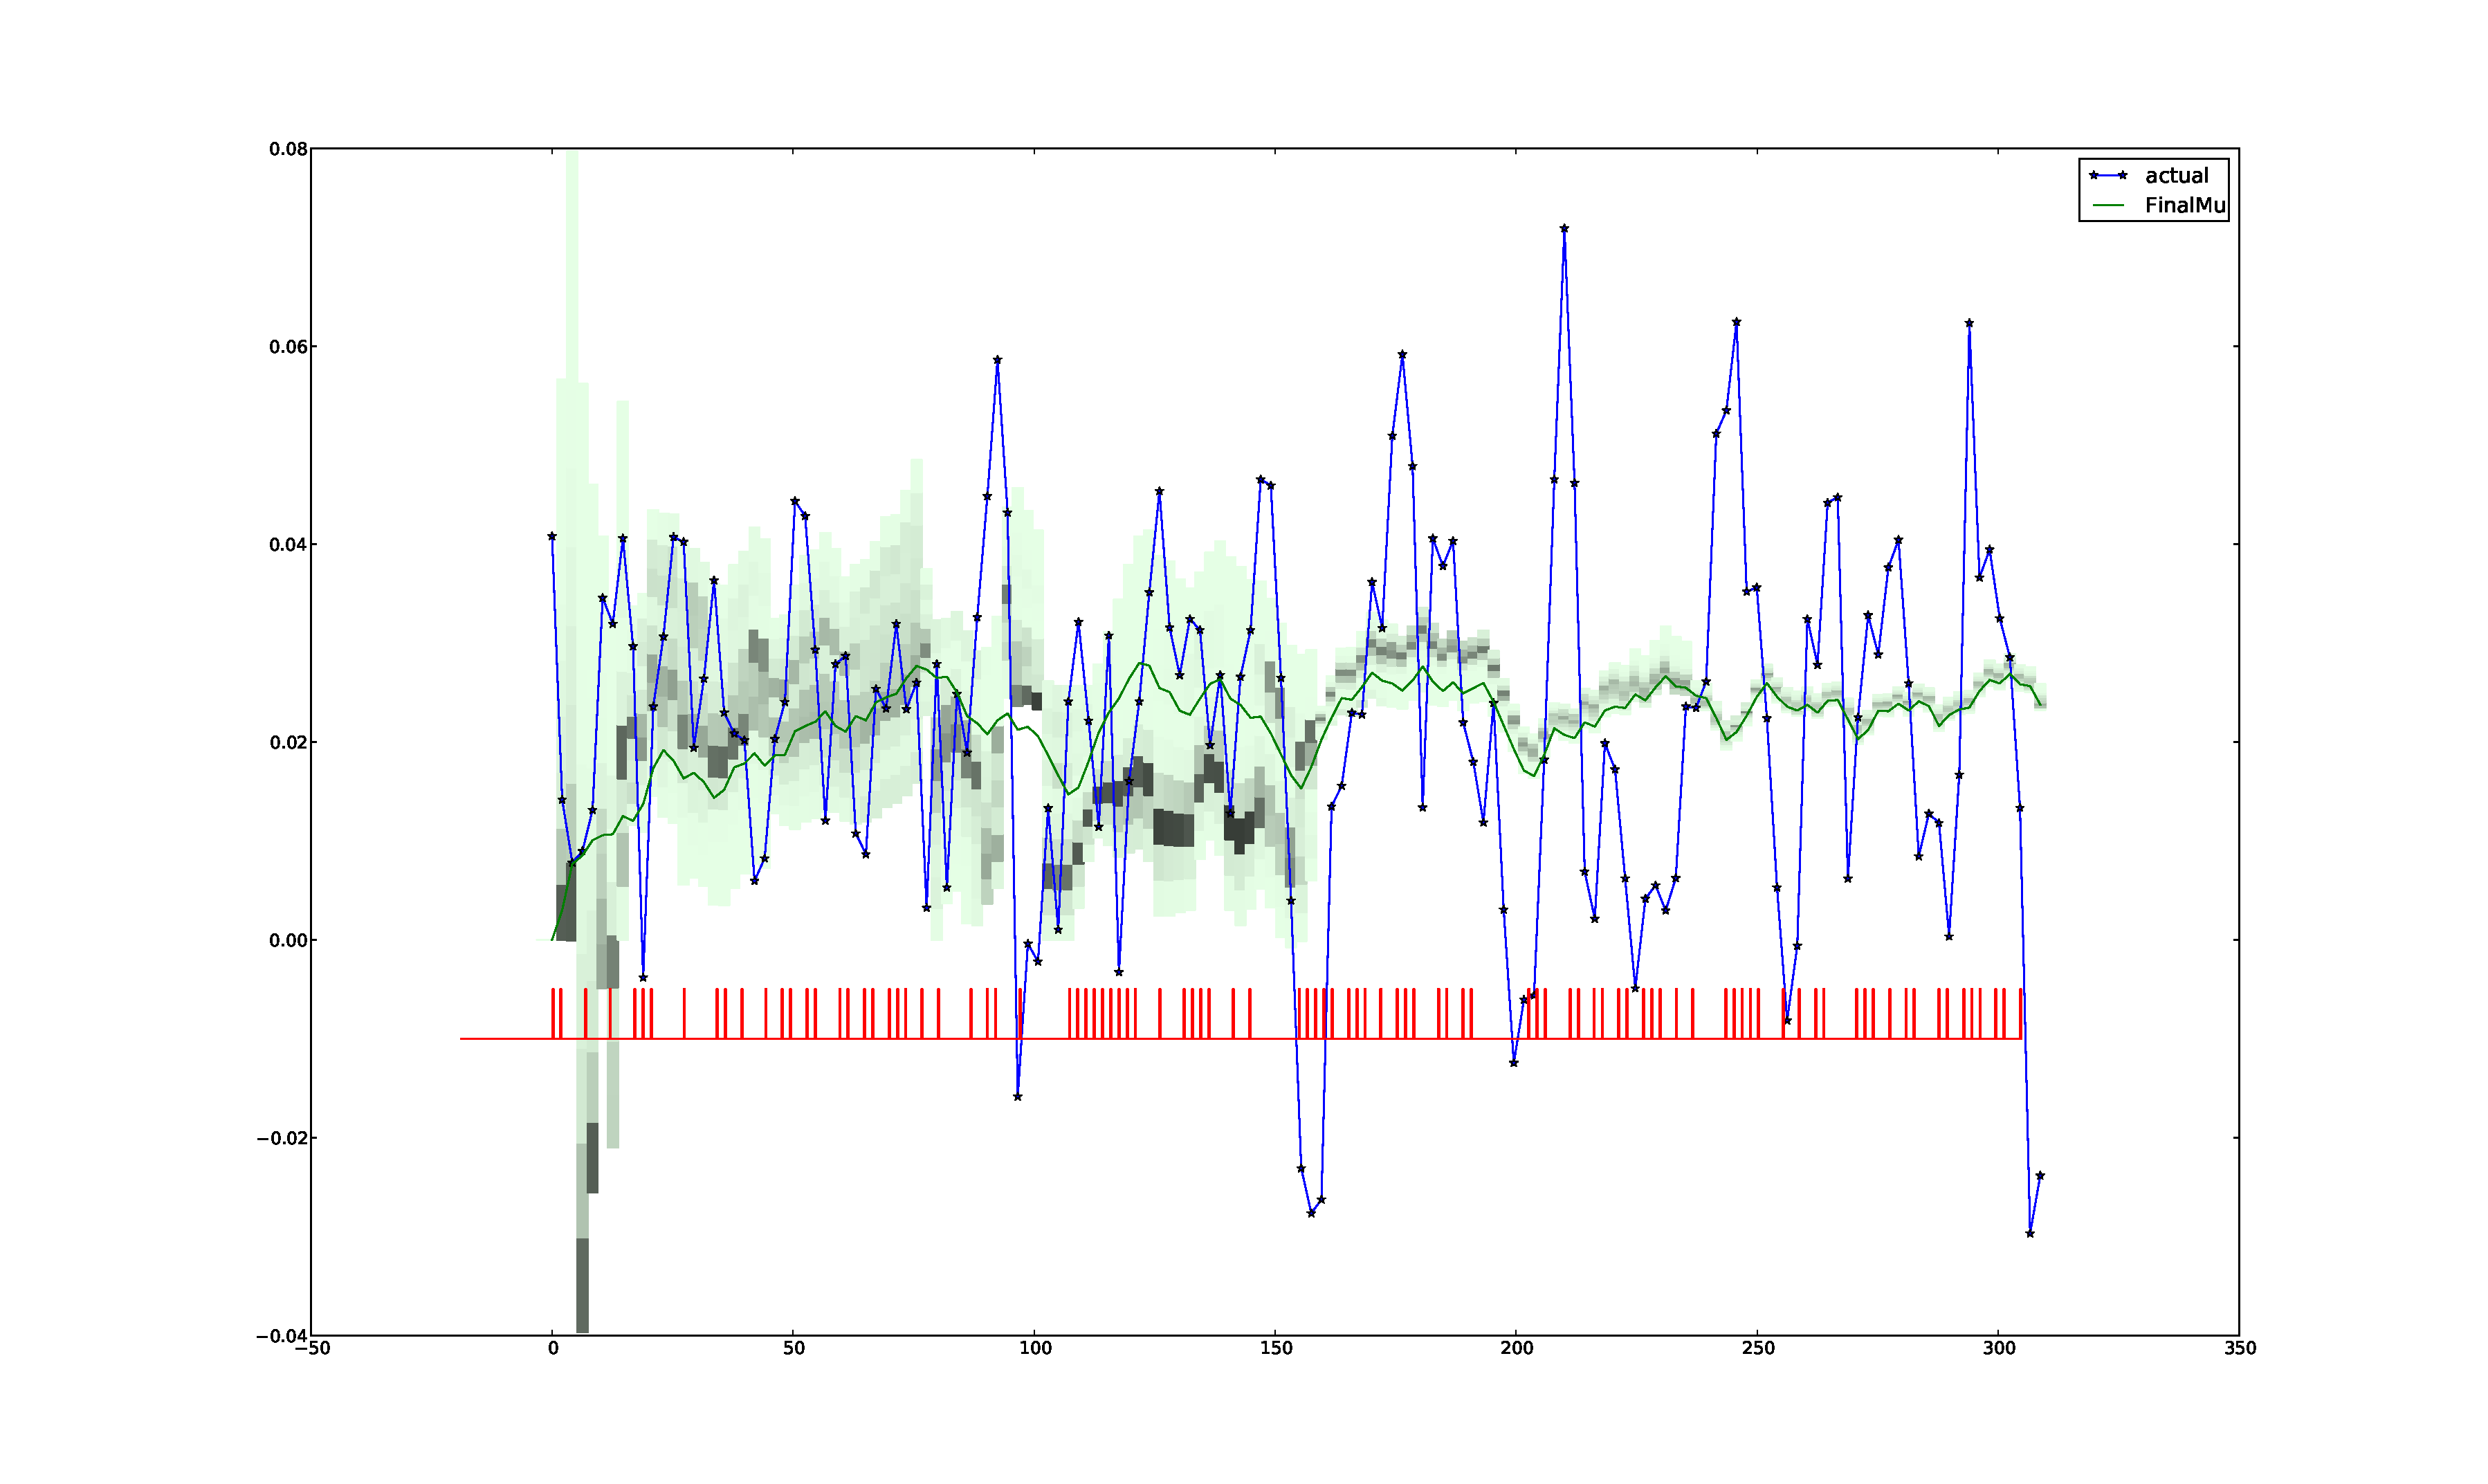
\includegraphics[trim=10cm 4cm 10cm 4cm, width=16cm]{images/inactive_illogical}
\caption{Particle Filter converging to values that make little sense,
because the voxel did not correlate with the input in any known way}
\end{figure}

\begin{figure}
\label{fig:highhard}
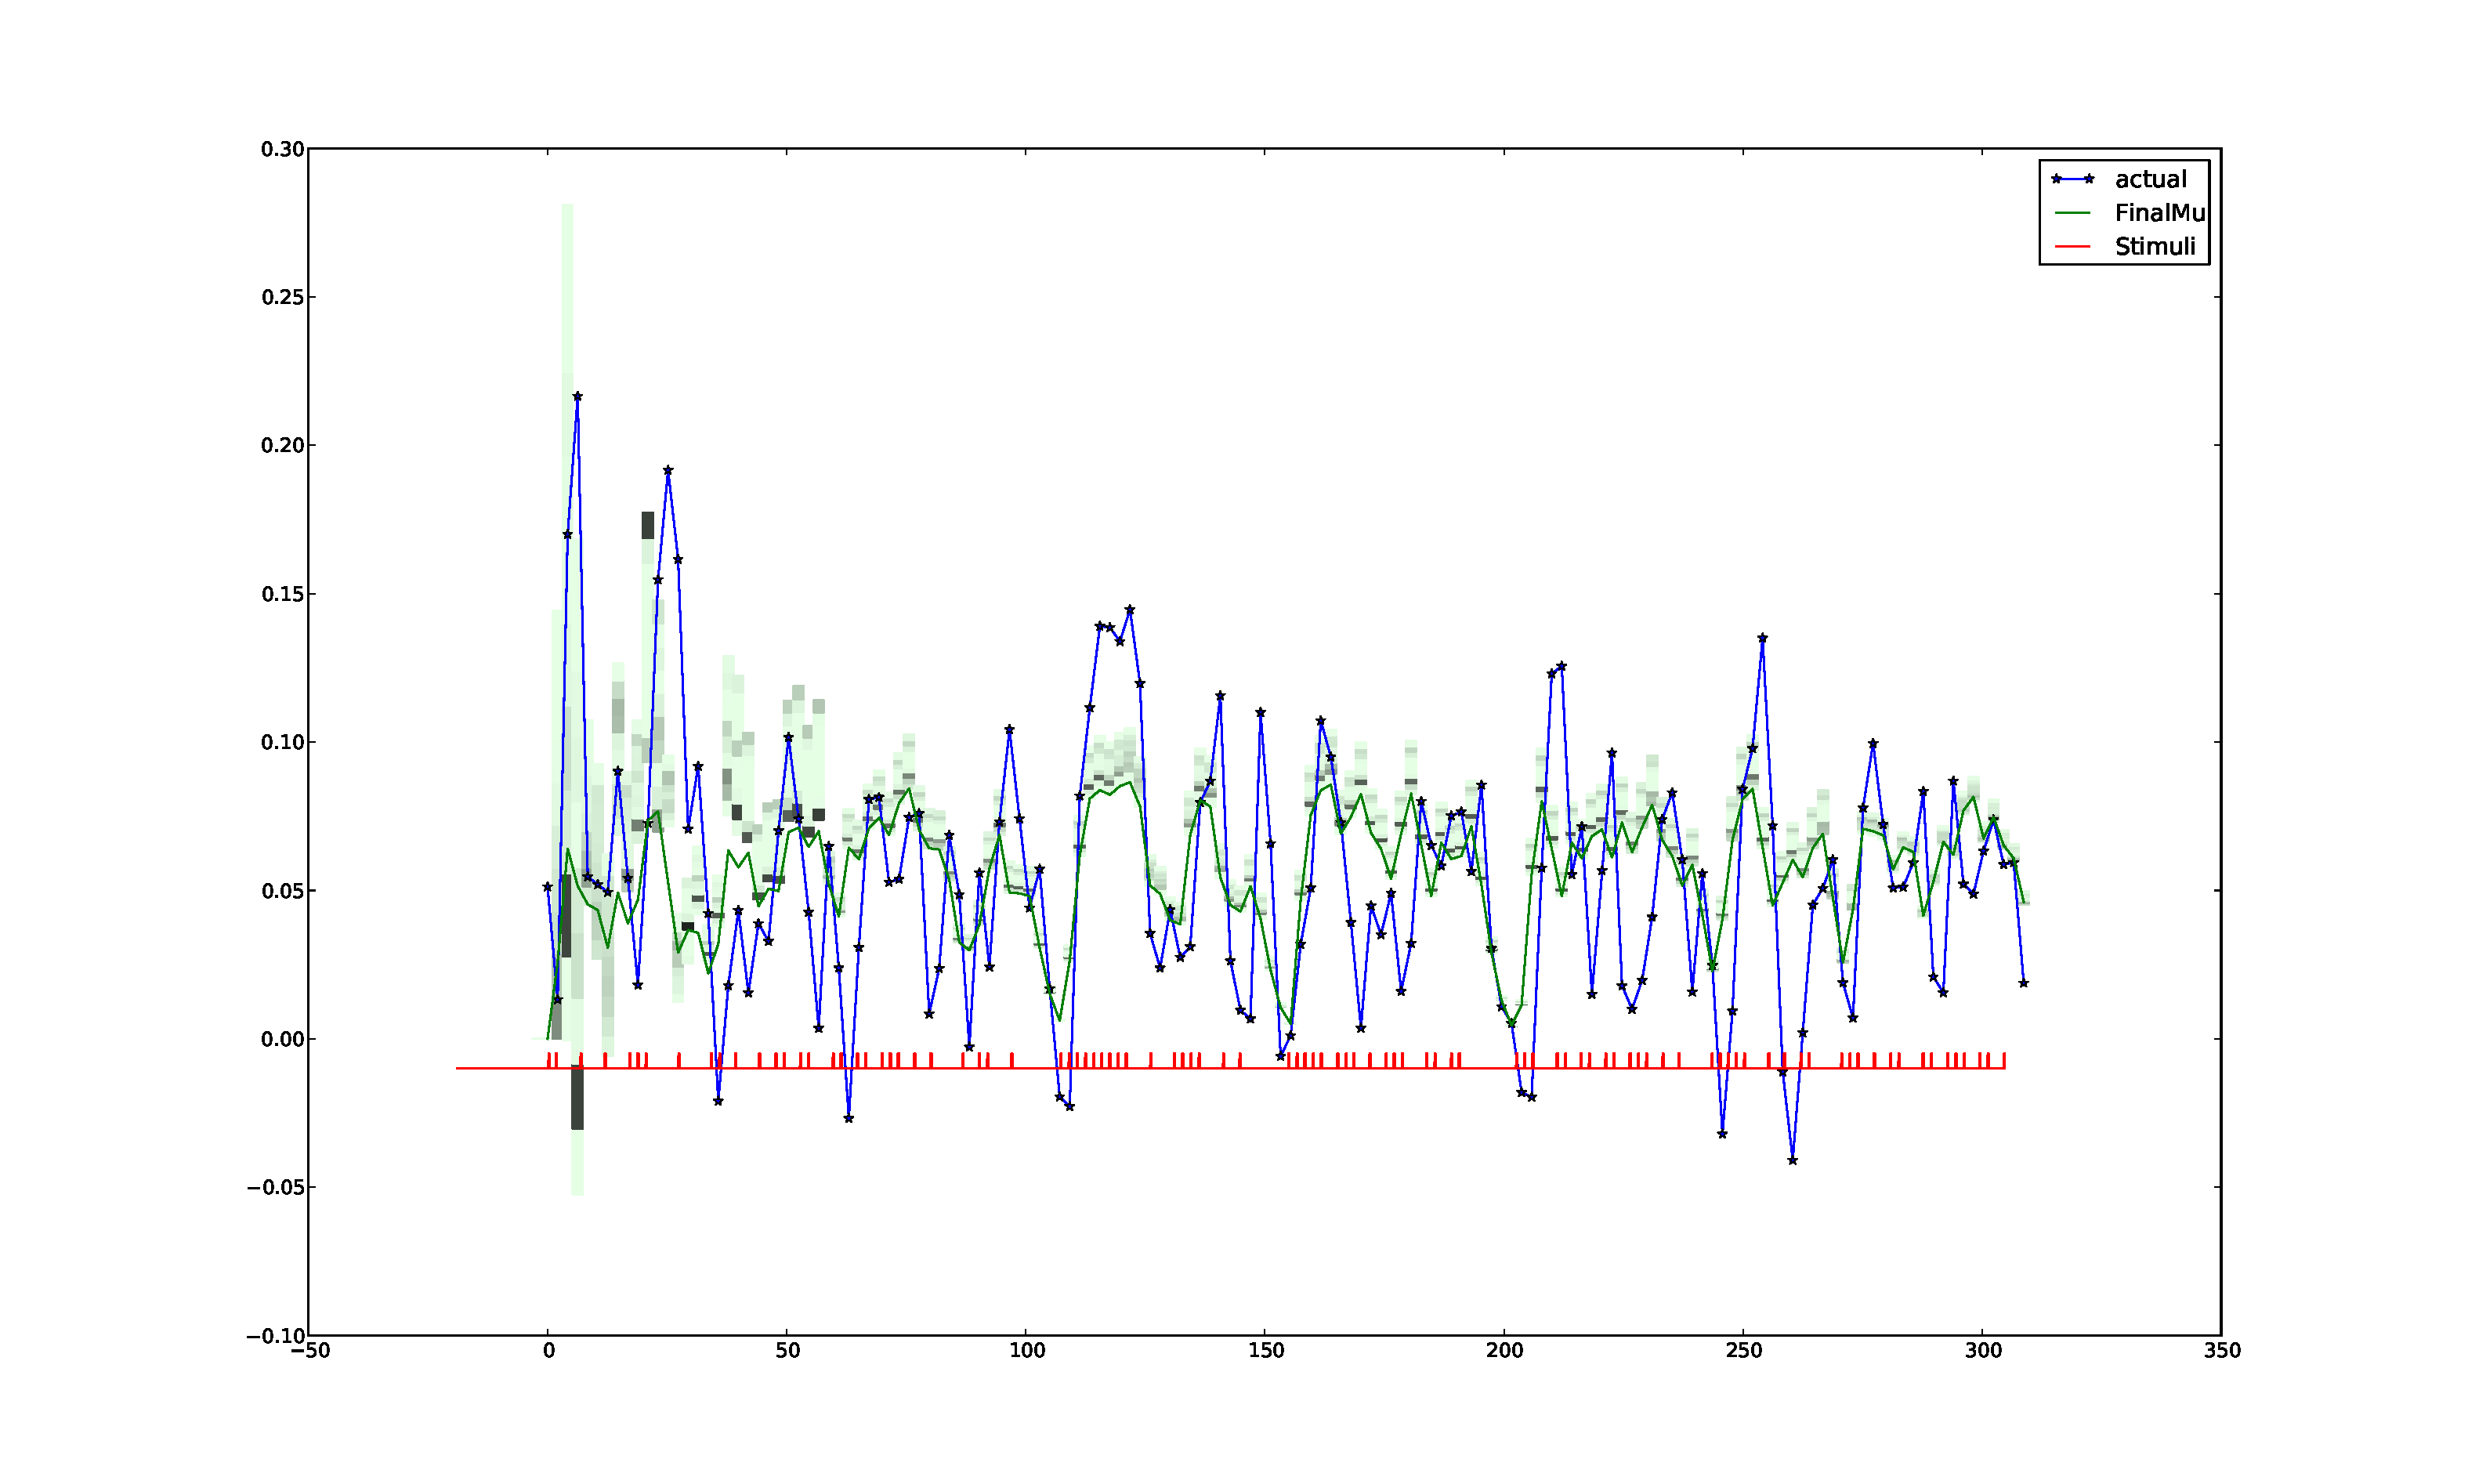
\includegraphics[trim=10cm 4cm 10cm 4cm, width=16cm]{images/active_difficult}
\caption{Example of a timeseries that laplace performs better on than
gaussian. The large spike at the beginning can quickly eliminate all particles} 

\end{figure}

For this reason, it is important to threshold based on the MSE, and the
impulse response. Naturally the MSE is intended to catch very voxels with a
very poor fit,
but like \autoref{fig:badfit}, the algorithm may have found a line
down the middle that gives a decent mean squared error. In this case
the excessive smoothing and low actual activation level will easily
be distinguished by finding the peak response to single short pulse. 

The choice of a prior, as discussed previously, is extremely important. While a
prior may have the potential to give good results, being a monte-carlo algorithm
there is the possibility for inconsistencies. Thus, increasing the variance
of the time-constants may allow additional flexibility, it will also cause
additional model variance. Case in point, the exact same algorithm run twice
with standard deviations of $.35, .35, .35$ for the time constants resulted in two
very different fits, see \autoref{fig:param1_var}.

\begin{figure}
\label{fig:badfit_param1}
\subfigure[]{\includegraphics{images/badfit_param1}}
\subfigure[]{\includegraphics{images/goodfit_param1}}
\caption{The same priors gave rise to both fits. Params: ($\tau_0 \alpha E_0 V_0 \tau_f \tau_s \epsilon$)
for the good fit: $(1.40 .32 0.34 0.04  0.96 2.76)$, and for the poor fit:
$(2.28 0.32 0.33 0.017 0.67 2.88 1.36)$.}
\end{figure}

For this reason, I actually lowered the standard deviattions of the time
constants to prevent over-smoothing. This resulted in the more consistent, but
slightly worse results seen in \autoref{fig:param2_var}

\begin{figure}
\label{fig:param2_var}
\subfigure[]{\includegraphics{images/param2a}}
\subfigure[]{\includegraphics{images/param2b}}
\caption{A poor fit, using the same parameters as }
\end{figure}

\section{Particle Collapse Recovery}
This heuristic was initially intended to deal with cases where the particle
filter prematurely converged; and to reverse this effect. In reality, however
it did not perform well, and so it was not used in full-brain analysis. Ultimately
it did not prevent collapse of the distribution, and it often caused dramatic
increased in the variance of parameter estimates. It also pronged the analysis
time of inactive time series. Essentially the effect was exactly opposite of what
one would hope.


\section{Weighting Function Comparison}
\label{sec:Results Weights}

\section{Single Time-Series Simulation}

Graphs: 

For simulated data, single timeseries:

For \{delta, DC/Spline\}, \{exponential, gaussian, cauchy\}, \{biased, unbiased initial\},
\{100, 500, 1000\} particles
\begin{enumerate}
\item Ground truth vs. Estimated signal during particle filter run
\item Ground truth vs. Estimated signal with final parameter set
\item True Parameters vs. Final Parameter Sets
\item Variance of final parameters when faced with same ground truth, different noise
\item MSE of (a new timeseries based on X(t) vs. ground truth) for all t
\item Estimator Variance based on different noise runs
\item Final Particle Distribution
\end{enumerate}

For Simulated Data, Full Volume:

%note to self, epsilon should probably be uniform between 0 and something
\section{Simulated Volume}
\begin{enumerate}
\item Parameter Map 
\item Error map of parameters
\item Histogram of \%errors between parameters
\item Activation Map based on a single region with high $\epsilon$, compared with linear
\end{enumerate}

Final parameter distribution among active regions.
Q-Q plots?

\section{FMRI Data}
....

image comparing epsilon-map with GLM activation map



\section{Conclusion}
\begin{frame}{Conclusion}
\begin{itemize}
    \item Summary:
    \begin{itemize}
    \item BOLD Parameters Ill-Defined
    \item Particle Filter Capable of good parameter BOLD estimate with 1000 particles
    \item Mutual Information performs well as estimate of Quality
    \end{itemize}
    \item Future Works
    \begin{itemize}
        \item Further limitations should be placed on priors, Deneux 
            et al. \cite{Deneux2006} shows that parameters could imposed.
        \item Analysis of joint parameter distribution for populations
        \item Real Time analysis possible for multiple Voxels, similar to
            De Charms et al. \cite{DeCharms2005}

    \end{itemize}
\end{itemize}
\end{frame}

\begin{frame}{Questions?}
\end{frame}

%% All of the following is optional and typically not needed. 
%\appendix
%\section<presentation>*{\appendixname}
%\subsection<presentation>*{For Further Reading}

\appendix

\section{Backup}
\begin{frame}{Balloon Flowchart}
\begin{figure}
\includegraphics[width=\textwidth]{backup_balloon}
\end{figure}
\end{frame}

\begin{frame}{SPM vs. Mutual Information Map, SPM}
\begin{figure}
\setcounter{subfigure}{0}
\subfigure[SPM Results]{\includegraphics[width=.8\textwidth]{images/spm_hm}}
\subfigure{\includegraphics[scale=.5]{images/scale1}}
\note{SPM results. Units of activation are in Student's $t$-scores; higher 
        indicates higher assurance that the signal cannot have occurred 
        through noise alone.}
\end{figure}
\end{frame}

\begin{frame}{SPM vs. Mutual Information Map, $M.I. > .15$}
\begin{figure}
\setcounter{subfigure}{1}
\subfigure[Particle Filter Results]{\includegraphics[width=.8\textwidth]{hm_mi_strict}}
\subfigure{\includegraphics[width=.1\textwidth]{scale4}}
\note{Particle filter results. Units of activation are in mutual information;
    higher indicates more assured activation.}
\end{figure}
\end{frame}

\begin{frame}{SPM vs. Mutual Information Map, $M.I. > .1$}
\begin{figure}
\setcounter{subfigure}{2}
\subfigure[Particle Filter Results]{\includegraphics[width=.8\textwidth]{mi_hm}}
\subfigure{\includegraphics[width=.1\textwidth]{scale6}}
\note{Particle filter results. Units of activation are in mutual information;
    higher indicates more assured activation.}
\end{figure}
\end{frame}

\begin{frame}{1: 37-14-7}
\setcounter{subfigure}{0}
\begin{figure}
\centering
\subfigure[Particle Filter]{\label{fig:comp1pfilter} \includegraphics[clip=true,trim=5cm 1cm 4cm 1cm,width=.4\textwidth]{images/1_pfilter_37_14_7}}
\subfigure[SPM]{\label{fig:comp1spm} \includegraphics[clip=true,trim=5cm 1cm 4cm 1cm,width=.4\textwidth]{images/1_spm_37_14_7}}
\caption{Section 1, Estimated vs. Actual BOLD response. $t$-Score: $10.71$, Mutual Information: $0.33$, Residual: $0.72$.}
\label{fig:comp1}
\end{figure}
\end{frame}

\begin{frame}{2: 34-12-7}
\setcounter{subfigure}{0}
\begin{figure}
\centering
\subfigure[Particle Filter]{\label{fig:comp2pfilter} \includegraphics[clip=true,trim=5cm 1cm 4cm 1cm,width=.4\textwidth]{images/2_pfilter_34_12_7}}
\subfigure[SPM]{\label{fig:comp2spm} \includegraphics[clip=true,trim=5cm 1cm 4cm 1cm,width=.4\textwidth]{images/2_spm_34_12_7}}
\caption{Section 2, Estimated vs. Actual BOLD response. $t$-Score: $6.97$, Mutual Information: $0.04$, Residual: $1.02$.}
\label{fig:comp2}
\end{figure}
\end{frame}

\begin{frame}{3: 23-21-7}
\setcounter{subfigure}{0}
\begin{figure}
\centering
\subfigure[Particle Filter]{\label{fig:comp3pfilter} \includegraphics[clip=true,trim=5cm 1cm 4cm 1cm,width=.4\textwidth]{images/3_pfilter_23_21_7}}
\subfigure[SPM]{\label{fig:comp3spm} \includegraphics[clip=true,trim=5cm 1cm 4cm 1cm,width=.4\textwidth]{images/3_spm_23_21_7}}
\caption{Section 3, Estimated vs. Actual BOLD response. $t$-Score: $2.85$, Mutual Information: $-0.03$, Residual: $0.81$.}
\label{fig:comp3}
\end{figure}
\end{frame}

\begin{frame}{4: 33-40-4}
\setcounter{subfigure}{0}
\begin{figure}
\centering
\subfigure[Particle Filter]{\label{fig:comp4pfilter} \includegraphics[clip=true,trim=5cm 1cm 4cm 1cm,width=.4\textwidth]{images/4_pfilter_26_15_7}}
\subfigure[SPM]{\label{fig:comp4spm} \includegraphics[clip=true,trim=5cm 1cm 4cm 1cm,width=.4\textwidth]{images/4_spm_26_15_7}}
\caption{Section 4, Estimated vs. Actual BOLD response. $t$-Score: $0.50$, Mutual Information: $0.06$, Residual: $0.95$. }
\label{fig:comp4}
\end{figure}
\end{frame}

\begin{frame}{5: 29-9-13}
\setcounter{subfigure}{0}
\begin{figure}
\centering
\subfigure[Particle Filter]{\label{fig:comp5pfilter} \includegraphics[clip=true,trim=5cm 1cm 4cm 1cm,width=.4\textwidth]{images/5_pfilter_29_9_13}}
\subfigure[SPM]{\label{fig:comp5spm} \includegraphics[clip=true,trim=5cm 1cm 4cm 1cm,width=.4\textwidth]{images/5_spm_29_9_13}}
\caption{Section 5, Estimated vs. Actual BOLD Response. $t$-Score: $4.17$, Mutual Information: $0.02$, Residual: $1.14$.}
%\caption{Section 5, Below threshold in both particle filter checks, but above threshold in SPM. Mutual Information of $0.0212822$, $t$-Value
%of $4.17399$ and $MSE$ of $1.14171$.}
\label{fig:comp5}
\end{figure}
\end{frame}

\begin{frame}{6: 36-17-19}
\setcounter{subfigure}{0}
\begin{figure}
\centering
\subfigure[Particle Filter]{\includegraphics[clip=true,trim=5cm 1cm 4cm 1cm,width=.4\textwidth]{images/6_pfilter_36_17_19}}
\subfigure[SPM]{\includegraphics[clip=true,trim=5cm 1cm 4cm 1cm,width=.4\textwidth]{images/6_spm_36_17_19}}
\caption{Section 6, Estimated vs. Actual BOLD Response. $t$-Score: $2.49$, Mutual Information: $.34$, Residual: $0.78$.}
%\caption{Section 6, MI of $0.335504$, T Value: $2.49154$, normalized error: $0.783348$ Not visible in SPM}
\end{figure}
\end{frame}

\begin{frame}{Particle Filter Results: Histogram}
\begin{figure}
\centering
\includegraphics[clip=truew,trim=8cm 4cm 8cm 4cm,width=.8\textwidth]{realhist}
\note{Histogram of parameters in active regions ($M.I. > .15$).}
\end{figure}
\end{frame}

\section{Bibliography}
\begin{frame}[allowframebreaks]
  \bibliographystyle{plain}
  \bibliography{../library}
\end{frame}


\end{document}



